%%%%%%%% ICML 2020 EXAMPLE LATEX SUBMISSION FILE %%%%%%%%%%%%%%%%%

\documentclass{article}

% Recommended, but optional, packages for figures and better typesetting:
\usepackage{microtype}
\usepackage{graphicx}
\usepackage{subcaption} % CHANGED: SUBFIGURE IS OUTDATED I CHANGED IT TO SUBCAPTION
\usepackage{booktabs} % for professional tables

% hyperref makes hyperlinks in the resulting PDF.
% If your build breaks (sometimes temporarily if a hyperlink spans a page)
% please comment out the following usepackage line and replace
% \usepackage{icml2020} with \usepackage[nohyperref]{icml2020} above.
\usepackage{hyperref}

% Attempt to make hyperref and algorithmic work together better:
\newcommand{\theHalgorithm}{\arabic{algorithm}}

% Use the following line for the initial blind version submitted for review:
%\usepackage{icml2021}

% If accepted, instead use the following line for the camera-ready submission:
\usepackage[accepted]{icml2021}


% 9 pages without references (camera ready)


%%%%% NEW MATH DEFINITIONS %%%%%

\usepackage{amsmath,amsfonts,bm}

% Mark sections of captions for referring to divisions of figures
\newcommand{\figleft}{{\em (Left)}}
\newcommand{\figcenter}{{\em (Center)}}
\newcommand{\figright}{{\em (Right)}}
\newcommand{\figtop}{{\em (Top)}}
\newcommand{\figbottom}{{\em (Bottom)}}
\newcommand{\captiona}{{\em (a)}}
\newcommand{\captionb}{{\em (b)}}
\newcommand{\captionc}{{\em (c)}}
\newcommand{\captiond}{{\em (d)}}

% Highlight a newly defined term
\newcommand{\newterm}[1]{{\bf #1}}


% Figure reference, lower-case.
\def\figref#1{figure~\ref{#1}}
% Figure reference, capital. For start of sentence
\def\Figref#1{Figure~\ref{#1}}
\def\twofigref#1#2{figures \ref{#1} and \ref{#2}}
\def\quadfigref#1#2#3#4{figures \ref{#1}, \ref{#2}, \ref{#3} and \ref{#4}}
% Section reference, lower-case.
\def\secref#1{section~\ref{#1}}
% Section reference, capital.
\def\Secref#1{Section~\ref{#1}}
% Reference to two sections.
\def\twosecrefs#1#2{sections \ref{#1} and \ref{#2}}
% Reference to three sections.
\def\secrefs#1#2#3{sections \ref{#1}, \ref{#2} and \ref{#3}}
% Reference to an equation, lower-case.
\def\eqref#1{equation~\ref{#1}}
% Reference to an equation, upper case
\def\Eqref#1{Equation~\ref{#1}}
% A raw reference to an equation---avoid using if possible
\def\plaineqref#1{\ref{#1}}
% Reference to a chapter, lower-case.
\def\chapref#1{chapter~\ref{#1}}
% Reference to an equation, upper case.
\def\Chapref#1{Chapter~\ref{#1}}
% Reference to a range of chapters
\def\rangechapref#1#2{chapters\ref{#1}--\ref{#2}}
% Reference to an algorithm, lower-case.
\def\algref#1{algorithm~\ref{#1}}
% Reference to an algorithm, upper case.
\def\Algref#1{Algorithm~\ref{#1}}
\def\twoalgref#1#2{algorithms \ref{#1} and \ref{#2}}
\def\Twoalgref#1#2{Algorithms \ref{#1} and \ref{#2}}
% Reference to a part, lower case
\def\partref#1{part~\ref{#1}}
% Reference to a part, upper case
\def\Partref#1{Part~\ref{#1}}
\def\twopartref#1#2{parts \ref{#1} and \ref{#2}}

\def\ceil#1{\lceil #1 \rceil}
\def\floor#1{\lfloor #1 \rfloor}
\def\1{\bm{1}}
\newcommand{\train}{\mathcal{D}}
\newcommand{\valid}{\mathcal{D_{\mathrm{valid}}}}
\newcommand{\test}{\mathcal{D_{\mathrm{test}}}}

\def\eps{{\epsilon}}


% Random variables
\def\reta{{\textnormal{$\eta$}}}
\def\ra{{\textnormal{a}}}
\def\rb{{\textnormal{b}}}
\def\rc{{\textnormal{c}}}
\def\rd{{\textnormal{d}}}
\def\re{{\textnormal{e}}}
\def\rf{{\textnormal{f}}}
\def\rg{{\textnormal{g}}}
\def\rh{{\textnormal{h}}}
\def\ri{{\textnormal{i}}}
\def\rj{{\textnormal{j}}}
\def\rk{{\textnormal{k}}}
\def\rl{{\textnormal{l}}}
% rm is already a command, just don't name any random variables m
\def\rn{{\textnormal{n}}}
\def\ro{{\textnormal{o}}}
\def\rp{{\textnormal{p}}}
\def\rq{{\textnormal{q}}}
\def\rr{{\textnormal{r}}}
\def\rs{{\textnormal{s}}}
\def\rt{{\textnormal{t}}}
\def\ru{{\textnormal{u}}}
\def\rv{{\textnormal{v}}}
\def\rw{{\textnormal{w}}}
\def\rx{{\textnormal{x}}}
\def\ry{{\textnormal{y}}}
\def\rz{{\textnormal{z}}}

% Random vectors
\def\rvepsilon{{\mathbf{\epsilon}}}
\def\rvtheta{{\mathbf{\theta}}}
\def\rva{{\mathbf{a}}}
\def\rvb{{\mathbf{b}}}
\def\rvc{{\mathbf{c}}}
\def\rvd{{\mathbf{d}}}
\def\rve{{\mathbf{e}}}
\def\rvf{{\mathbf{f}}}
\def\rvg{{\mathbf{g}}}
\def\rvh{{\mathbf{h}}}
\def\rvu{{\mathbf{i}}}
\def\rvj{{\mathbf{j}}}
\def\rvk{{\mathbf{k}}}
\def\rvl{{\mathbf{l}}}
\def\rvm{{\mathbf{m}}}
\def\rvn{{\mathbf{n}}}
\def\rvo{{\mathbf{o}}}
\def\rvp{{\mathbf{p}}}
\def\rvq{{\mathbf{q}}}
\def\rvr{{\mathbf{r}}}
\def\rvs{{\mathbf{s}}}
\def\rvt{{\mathbf{t}}}
\def\rvu{{\mathbf{u}}}
\def\rvv{{\mathbf{v}}}
\def\rvw{{\mathbf{w}}}
\def\rvx{{\mathbf{x}}}
\def\rvy{{\mathbf{y}}}
\def\rvz{{\mathbf{z}}}

% Elements of random vectors
\def\erva{{\textnormal{a}}}
\def\ervb{{\textnormal{b}}}
\def\ervc{{\textnormal{c}}}
\def\ervd{{\textnormal{d}}}
\def\erve{{\textnormal{e}}}
\def\ervf{{\textnormal{f}}}
\def\ervg{{\textnormal{g}}}
\def\ervh{{\textnormal{h}}}
\def\ervi{{\textnormal{i}}}
\def\ervj{{\textnormal{j}}}
\def\ervk{{\textnormal{k}}}
\def\ervl{{\textnormal{l}}}
\def\ervm{{\textnormal{m}}}
\def\ervn{{\textnormal{n}}}
\def\ervo{{\textnormal{o}}}
\def\ervp{{\textnormal{p}}}
\def\ervq{{\textnormal{q}}}
\def\ervr{{\textnormal{r}}}
\def\ervs{{\textnormal{s}}}
\def\ervt{{\textnormal{t}}}
\def\ervu{{\textnormal{u}}}
\def\ervv{{\textnormal{v}}}
\def\ervw{{\textnormal{w}}}
\def\ervx{{\textnormal{x}}}
\def\ervy{{\textnormal{y}}}
\def\ervz{{\textnormal{z}}}

% Random matrices
\def\rmA{{\mathbf{A}}}
\def\rmB{{\mathbf{B}}}
\def\rmC{{\mathbf{C}}}
\def\rmD{{\mathbf{D}}}
\def\rmE{{\mathbf{E}}}
\def\rmF{{\mathbf{F}}}
\def\rmG{{\mathbf{G}}}
\def\rmH{{\mathbf{H}}}
\def\rmI{{\mathbf{I}}}
\def\rmJ{{\mathbf{J}}}
\def\rmK{{\mathbf{K}}}
\def\rmL{{\mathbf{L}}}
\def\rmM{{\mathbf{M}}}
\def\rmN{{\mathbf{N}}}
\def\rmO{{\mathbf{O}}}
\def\rmP{{\mathbf{P}}}
\def\rmQ{{\mathbf{Q}}}
\def\rmR{{\mathbf{R}}}
\def\rmS{{\mathbf{S}}}
\def\rmT{{\mathbf{T}}}
\def\rmU{{\mathbf{U}}}
\def\rmV{{\mathbf{V}}}
\def\rmW{{\mathbf{W}}}
\def\rmX{{\mathbf{X}}}
\def\rmY{{\mathbf{Y}}}
\def\rmZ{{\mathbf{Z}}}

% Elements of random matrices
\def\ermA{{\textnormal{A}}}
\def\ermB{{\textnormal{B}}}
\def\ermC{{\textnormal{C}}}
\def\ermD{{\textnormal{D}}}
\def\ermE{{\textnormal{E}}}
\def\ermF{{\textnormal{F}}}
\def\ermG{{\textnormal{G}}}
\def\ermH{{\textnormal{H}}}
\def\ermI{{\textnormal{I}}}
\def\ermJ{{\textnormal{J}}}
\def\ermK{{\textnormal{K}}}
\def\ermL{{\textnormal{L}}}
\def\ermM{{\textnormal{M}}}
\def\ermN{{\textnormal{N}}}
\def\ermO{{\textnormal{O}}}
\def\ermP{{\textnormal{P}}}
\def\ermQ{{\textnormal{Q}}}
\def\ermR{{\textnormal{R}}}
\def\ermS{{\textnormal{S}}}
\def\ermT{{\textnormal{T}}}
\def\ermU{{\textnormal{U}}}
\def\ermV{{\textnormal{V}}}
\def\ermW{{\textnormal{W}}}
\def\ermX{{\textnormal{X}}}
\def\ermY{{\textnormal{Y}}}
\def\ermZ{{\textnormal{Z}}}

% Vectors
\def\vzero{{\bm{0}}}
\def\vone{{\bm{1}}}
\def\vmu{{\bm{\mu}}}
\def\vtheta{{\bm{\theta}}}
\def\va{{\bm{a}}}
\def\vb{{\bm{b}}}
\def\vc{{\bm{c}}}
\def\vd{{\bm{d}}}
\def\ve{{\bm{e}}}
\def\vf{{\bm{f}}}
\def\vg{{\bm{g}}}
\def\vh{{\bm{h}}}
\def\vi{{\bm{i}}}
\def\vj{{\bm{j}}}
\def\vk{{\bm{k}}}
\def\vl{{\bm{l}}}
\def\vm{{\bm{m}}}
\def\vn{{\bm{n}}}
\def\vo{{\bm{o}}}
\def\vp{{\bm{p}}}
\def\vq{{\bm{q}}}
\def\vr{{\bm{r}}}
\def\vs{{\bm{s}}}
\def\vt{{\bm{t}}}
\def\vu{{\bm{u}}}
\def\vv{{\bm{v}}}
\def\vw{{\bm{w}}}
\def\vx{{\bm{x}}}
\def\vy{{\bm{y}}}
\def\vz{{\bm{z}}}

% Elements of vectors
\def\evalpha{{\alpha}}
\def\evbeta{{\beta}}
\def\evepsilon{{\epsilon}}
\def\evlambda{{\lambda}}
\def\evomega{{\omega}}
\def\evmu{{\mu}}
\def\evpsi{{\psi}}
\def\evsigma{{\sigma}}
\def\evtheta{{\theta}}
\def\eva{{a}}
\def\evb{{b}}
\def\evc{{c}}
\def\evd{{d}}
\def\eve{{e}}
\def\evf{{f}}
\def\evg{{g}}
\def\evh{{h}}
\def\evi{{i}}
\def\evj{{j}}
\def\evk{{k}}
\def\evl{{l}}
\def\evm{{m}}
\def\evn{{n}}
\def\evo{{o}}
\def\evp{{p}}
\def\evq{{q}}
\def\evr{{r}}
\def\evs{{s}}
\def\evt{{t}}
\def\evu{{u}}
\def\evv{{v}}
\def\evw{{w}}
\def\evx{{x}}
\def\evy{{y}}
\def\evz{{z}}

% Matrix
\def\mA{{\bm{A}}}
\def\mB{{\bm{B}}}
\def\mC{{\bm{C}}}
\def\mD{{\bm{D}}}
\def\mE{{\bm{E}}}
\def\mF{{\bm{F}}}
\def\mG{{\bm{G}}}
\def\mH{{\bm{H}}}
\def\mI{{\bm{I}}}
\def\mJ{{\bm{J}}}
\def\mK{{\bm{K}}}
\def\mL{{\bm{L}}}
\def\mM{{\bm{M}}}
\def\mN{{\bm{N}}}
\def\mO{{\bm{O}}}
\def\mP{{\bm{P}}}
\def\mQ{{\bm{Q}}}
\def\mR{{\bm{R}}}
\def\mS{{\bm{S}}}
\def\mT{{\bm{T}}}
\def\mU{{\bm{U}}}
\def\mV{{\bm{V}}}
\def\mW{{\bm{W}}}
\def\mX{{\bm{X}}}
\def\mY{{\bm{Y}}}
\def\mZ{{\bm{Z}}}
\def\mBeta{{\bm{\beta}}}
\def\mPhi{{\bm{\Phi}}}
\def\mLambda{{\bm{\Lambda}}}
\def\mSigma{{\bm{\Sigma}}}

% Tensor
\DeclareMathAlphabet{\mathsfit}{\encodingdefault}{\sfdefault}{m}{sl}
\SetMathAlphabet{\mathsfit}{bold}{\encodingdefault}{\sfdefault}{bx}{n}
\newcommand{\tens}[1]{\bm{\mathsfit{#1}}}
\def\tA{{\tens{A}}}
\def\tB{{\tens{B}}}
\def\tC{{\tens{C}}}
\def\tD{{\tens{D}}}
\def\tE{{\tens{E}}}
\def\tF{{\tens{F}}}
\def\tG{{\tens{G}}}
\def\tH{{\tens{H}}}
\def\tI{{\tens{I}}}
\def\tJ{{\tens{J}}}
\def\tK{{\tens{K}}}
\def\tL{{\tens{L}}}
\def\tM{{\tens{M}}}
\def\tN{{\tens{N}}}
\def\tO{{\tens{O}}}
\def\tP{{\tens{P}}}
\def\tQ{{\tens{Q}}}
\def\tR{{\tens{R}}}
\def\tS{{\tens{S}}}
\def\tT{{\tens{T}}}
\def\tU{{\tens{U}}}
\def\tV{{\tens{V}}}
\def\tW{{\tens{W}}}
\def\tX{{\tens{X}}}
\def\tY{{\tens{Y}}}
\def\tZ{{\tens{Z}}}


% Graph
\def\gA{{\mathcal{A}}}
\def\gB{{\mathcal{B}}}
\def\gC{{\mathcal{C}}}
\def\gD{{\mathcal{D}}}
\def\gE{{\mathcal{E}}}
\def\gF{{\mathcal{F}}}
\def\gG{{\mathcal{G}}}
\def\gH{{\mathcal{H}}}
\def\gI{{\mathcal{I}}}
\def\gJ{{\mathcal{J}}}
\def\gK{{\mathcal{K}}}
\def\gL{{\mathcal{L}}}
\def\gM{{\mathcal{M}}}
\def\gN{{\mathcal{N}}}
\def\gO{{\mathcal{O}}}
\def\gP{{\mathcal{P}}}
\def\gQ{{\mathcal{Q}}}
\def\gR{{\mathcal{R}}}
\def\gS{{\mathcal{S}}}
\def\gT{{\mathcal{T}}}
\def\gU{{\mathcal{U}}}
\def\gV{{\mathcal{V}}}
\def\gW{{\mathcal{W}}}
\def\gX{{\mathcal{X}}}
\def\gY{{\mathcal{Y}}}
\def\gZ{{\mathcal{Z}}}

% Sets
\def\sA{{\mathbb{A}}}
\def\sB{{\mathbb{B}}}
\def\sC{{\mathbb{C}}}
\def\sD{{\mathbb{D}}}
% Don't use a set called E, because this would be the same as our symbol
% for expectation.
\def\sF{{\mathbb{F}}}
\def\sG{{\mathbb{G}}}
\def\sH{{\mathbb{H}}}
\def\sI{{\mathbb{I}}}
\def\sJ{{\mathbb{J}}}
\def\sK{{\mathbb{K}}}
\def\sL{{\mathbb{L}}}
\def\sM{{\mathbb{M}}}
\def\sN{{\mathbb{N}}}
\def\sO{{\mathbb{O}}}
\def\sP{{\mathbb{P}}}
\def\sQ{{\mathbb{Q}}}
\def\sR{{\mathbb{R}}}
\def\sS{{\mathbb{S}}}
\def\sT{{\mathbb{T}}}
\def\sU{{\mathbb{U}}}
\def\sV{{\mathbb{V}}}
\def\sW{{\mathbb{W}}}
\def\sX{{\mathbb{X}}}
\def\sY{{\mathbb{Y}}}
\def\sZ{{\mathbb{Z}}}

% Entries of a matrix
\def\emLambda{{\Lambda}}
\def\emA{{A}}
\def\emB{{B}}
\def\emC{{C}}
\def\emD{{D}}
\def\emE{{E}}
\def\emF{{F}}
\def\emG{{G}}
\def\emH{{H}}
\def\emI{{I}}
\def\emJ{{J}}
\def\emK{{K}}
\def\emL{{L}}
\def\emM{{M}}
\def\emN{{N}}
\def\emO{{O}}
\def\emP{{P}}
\def\emQ{{Q}}
\def\emR{{R}}
\def\emS{{S}}
\def\emT{{T}}
\def\emU{{U}}
\def\emV{{V}}
\def\emW{{W}}
\def\emX{{X}}
\def\emY{{Y}}
\def\emZ{{Z}}
\def\emSigma{{\Sigma}}

% entries of a tensor
% Same font as tensor, without \bm wrapper
\newcommand{\etens}[1]{\mathsfit{#1}}
\def\etLambda{{\etens{\Lambda}}}
\def\etA{{\etens{A}}}
\def\etB{{\etens{B}}}
\def\etC{{\etens{C}}}
\def\etD{{\etens{D}}}
\def\etE{{\etens{E}}}
\def\etF{{\etens{F}}}
\def\etG{{\etens{G}}}
\def\etH{{\etens{H}}}
\def\etI{{\etens{I}}}
\def\etJ{{\etens{J}}}
\def\etK{{\etens{K}}}
\def\etL{{\etens{L}}}
\def\etM{{\etens{M}}}
\def\etN{{\etens{N}}}
\def\etO{{\etens{O}}}
\def\etP{{\etens{P}}}
\def\etQ{{\etens{Q}}}
\def\etR{{\etens{R}}}
\def\etS{{\etens{S}}}
\def\etT{{\etens{T}}}
\def\etU{{\etens{U}}}
\def\etV{{\etens{V}}}
\def\etW{{\etens{W}}}
\def\etX{{\etens{X}}}
\def\etY{{\etens{Y}}}
\def\etZ{{\etens{Z}}}

% The true underlying data generating distribution
\newcommand{\pdata}{p_{\rm{data}}}
% The empirical distribution defined by the training set
\newcommand{\ptrain}{\hat{p}_{\rm{data}}}
\newcommand{\Ptrain}{\hat{P}_{\rm{data}}}
% The model distribution
\newcommand{\pmodel}{p_{\rm{model}}}
\newcommand{\Pmodel}{P_{\rm{model}}}
\newcommand{\ptildemodel}{\tilde{p}_{\rm{model}}}
% Stochastic autoencoder distributions
\newcommand{\pencode}{p_{\rm{encoder}}}
\newcommand{\pdecode}{p_{\rm{decoder}}}
\newcommand{\precons}{p_{\rm{reconstruct}}}

\newcommand{\laplace}{\mathrm{Laplace}} % Laplace distribution

\newcommand{\E}{\mathbb{E}}
\newcommand{\Ls}{\mathcal{L}}
\newcommand{\R}{\mathbb{R}}
\newcommand{\emp}{\tilde{p}}
\newcommand{\lr}{\alpha}
\newcommand{\reg}{\lambda}
\newcommand{\rect}{\mathrm{rectifier}}
\newcommand{\softmax}{\mathrm{softmax}}
\newcommand{\sigmoid}{\sigma}
\newcommand{\softplus}{\zeta}
\newcommand{\KL}{D_{\mathrm{KL}}}
\newcommand{\Var}{\mathrm{Var}}
\newcommand{\standarderror}{\mathrm{SE}}
\newcommand{\Cov}{\mathrm{Cov}}
% Wolfram Mathworld says $L^2$ is for function spaces and $\ell^2$ is for vectors
% But then they seem to use $L^2$ for vectors throughout the site, and so does
% wikipedia.
\newcommand{\normlzero}{L^0}
\newcommand{\normlone}{L^1}
\newcommand{\normltwo}{L^2}
\newcommand{\normlp}{L^p}
\newcommand{\normmax}{L^\infty}

\newcommand{\parents}{Pa} % See usage in notation.tex. Chosen to match Daphne's book.

\DeclareMathOperator*{\argmax}{arg\,max}
\DeclareMathOperator*{\argmin}{arg\,min}

\DeclareMathOperator{\sign}{sign}
\DeclareMathOperator{\Tr}{Tr}
\let\ab\allowbreak

\newcommand{\inputdim}{D}
\newcommand{\latentdim}{H}
\newcommand{\suffstatdim}{L}
\newcommand\idata{i\xspace}
\newcommand\ndata{N\xspace}
\newcommand\dataix{^{(\idata)}}
\newcommand\iclass{c\xspace}
\newcommand\nclass{C\xspace}

% additional packages
\usepackage{hyperref}       % hyperlinks
\usepackage{url}            % simple URL typesetting

\usepackage{amsmath}
\usepackage{amssymb}
\usepackage{amsfonts}       % blackboard math symbols
\usepackage{amsthm}
\usepackage{nicefrac}       % compact symbols for 1/2, etc.
\usepackage{microtype}      % microtypography

%\usepackage{xcolor}
\usepackage[utf8]{inputenc} % allow utf-8 input
\usepackage[T1]{fontenc}    % use 8-bit T1 fonts
\usepackage{bbold}
%\usepackage{tikz}
%\usepackage{xspace}
\usepackage{stmaryrd}
\usepackage{bm}

\usepackage{float}
\usepackage[inline]{enumitem}
\usepackage{caption} 
%\usepackage{subcaption}
\usepackage{wrapfig}
\usepackage{booktabs}
\usepackage{makecell}
\captionsetup[table]{skip=6pt}
%\usetikzlibrary{shapes, arrows}
\usepackage[table]{colortbl}
\usepackage{xspace}
\usepackage{multirow}

\usepackage{subfiles}
\providecommand{\main}{.}







% The \icmltitle you define below is probably too long as a header.
% Therefore, a short form for the running title is supplied here:
\icmltitlerunning{Evaluating Robustness of Predictive Uncertainty Estimation: Are Dirichlet-based Models Reliable?}

\DeclareMathOperator{\DNormal}{\mathcal{N}}

\newcommand\idata{i\xspace}
\newcommand\dataix{^{(\idata)}}
\newcommand\iclass{c\xspace}
\newcommand\nclass{C\xspace}
\newcommand\PriorNet{PriorNet\xspace}
\newcommand\RevPriorNet{RevPriorNet\xspace}
\newcommand\EvNet{EvNet\xspace}
\newcommand\DDNet{DDNet\xspace}
\newcommand\PostNet{PostNet\xspace}

\newcommand{\sg}[1]{\textcolor{magenta}{(SG: #1)}}
\newcommand{\ak}[1]{\textcolor{green}{(AK: #1)}}
\newcommand\bc[1]{\textcolor{green}{(BC: #1)}}
\newcommand\dz[1]{\textcolor{green}{(DZ: #1)}}




\begin{document}

\twocolumn[
\icmltitle{Evaluating Robustness of Predictive Uncertainty Estimation: \\ Are Dirichlet-based Models Reliable?}

% It is OKAY to include author information, even for blind
% submissions: the style file will automatically remove it for you
% unless you've provided the [accepted] option to the icml2020
% package.

% List of affiliations: The first argument should be a (short)
% identifier you will use later to specify author affiliations
% Academic affiliations should list Department, University, City, Region, Country
% Industry affiliations should list Company, City, Region, Country

% You can specify symbols, otherwise they are numbered in order.
% Ideally, you should not use this facility. Affiliations will be numbered
% in order of appearance and this is the preferred way.
\icmlsetsymbol{equal}{*}

\begin{icmlauthorlist}
\icmlauthor{Anna-Kathrin Kopetzki}{equal,tum}
\icmlauthor{Bertrand Charpentier}{equal,tum}
\icmlauthor{Daniel Z\"ugner}{tum}
\icmlauthor{Sandhya Giri}{tum}
\icmlauthor{Stephan G\"unnemann}{tum}
\end{icmlauthorlist}


  \hypersetup{ %
    pdftitle={Evaluating Robustness of Predictive Uncertainty Estimation: Are Dirichlet-based Models Reliable?},
    pdfauthor={Anna-Kathrin Kopetzki, Bertrand Charpentier, Daniel Z\"ugner, Sandhya Giri, Stephan G\"unnemann },
    pdfsubject={Proceedings of the International Conference on Machine Learning 2021},
    pdfkeywords={Uncertainty Estimation, Robustness},
}

% Publikationsrichtilinie TUM (Example): Technical University of Munich, Germany; School of Engineering \& Design, Department of Mechanical Engineering
%ours: TUM, Dep. of Informatics

\icmlaffiliation{tum}{Technical University of Munich, Germany; Department of Informatics}
%\icmlaffiliation{goo}{Googol ShallowMind, New London, Michigan, USA}
%\icmlaffiliation{ed}{School of Computation, University of Edenborrow, Edenborrow, United Kingdom}

\icmlcorrespondingauthor{Anna-Kathrin Kopetzki}{kopetzki@in.tum.de}
\icmlcorrespondingauthor{Bertrand Charpentier}{charpent@in.tum.de}

% You may provide any keywords that you
% find helpful for describing your paper; these are used to populate
% the "keywords" metadata in the PDF but will not be shown in the document
\icmlkeywords{Machine Learning, ICML}

\vskip 0.3in
]

% this must go after the closing bracket ] following \twocolumn[ ...

% This command actually creates the footnote in the first column
% listing the affiliations and the copyright notice.
% The command takes one argument, which is text to display at the start of the footnote.
% The \icmlEqualContribution command is standard text for equal contribution.
% Remove it (just {}) if you do not need this facility.

%\printAffiliationsAndNotice{}  % leave blank if no need to mention equal contribution
\printAffiliationsAndNotice{\icmlEqualContribution} % otherwise use the standard text.


\begin{abstract}
Dirichlet-based uncertainty (DBU) models are a recent and promising class of uncertainty-aware models. DBU models predict the parameters of a Dirichlet distribution to provide fast, high-quality uncertainty estimates alongside with class predictions. 
%
In this work, we present the first large-scale, in-depth study of the robustness of DBU models under adversarial attacks. Our results suggest that uncertainty estimates of DBU models are not robust w.r.t.\ three important tasks:
%
\textbf{(1)} indicating correctly and wrongly classified samples;
%
\textbf{ (2)} detecting adversarial examples; and 
%
\textbf{(3)} distinguishing between in-distribution (ID) and out-of-distribution (OOD) data.
%
Additionally, we explore the first approaches to make DBU models more robust. While adversarial training has a minor effect, our median smoothing based approach significantly increases robustness of DBU models. 

\end{abstract}

\section{Introduction}
\label{sec:introduction_008}

In \cref{chap:practicality}, we studied practical considerations when using efficient uncertainty estimation methods in non-adversarial contexts. In this chapter, we now focus on the robustness of uncertainty estimates in adversarial contexts.

Indeed, although neural networks achieve high predictive accuracy in many tasks, they are known to have two substantial weaknesses: First, neural networks are not robust against adversarial perturbations, i.e., semantically meaningless input changes that lead to wrong predictions \citep{szegedy2014, goodfellow2014}. 
Second, standard neural networks are unable to identify samples that are different from the ones they were trained on and tend to make over-confident predictions at test time \citep{ensembles}. These weaknesses make them impracticable in sensitive domains like financial, autonomous driving or medical areas which require trust in predictions.

To increase trust in neural networks, models that provide predictions along with the corresponding uncertainty have been proposed. In previous chapters we have seen \PostNetacro{} (see \cref{chap:classification}) and \NatPNacro{} (see \cref{chap:regression}) which, when applied to classification tasks, belong to the important family of Dirichlet-based uncertainty (DBU) models  \citep{malini2018, distribution-distillation, sensoy2018, reverse-kl, charpentier2020, graph_uncertainty, max_gap_id_ood, multifaceted_uncertainty, uncertainty-generative-classifier}. 
Contrary to other approaches such as Bayesian Neural Networks \citep{bayesian-networks, osawa2019, simple-baseline-uncertainty}, drop out \citep{dropout} or ensembles \citep{ensembles}, DBU models provide efficient uncertainty estimates at test time in a single forward pass by directly predicting the parameters of a Dirichlet distribution over categorical probability distributions.
%
%\begin{wrapfigure}{r}{0.4\textwidth}%[16]{r}{0cm}
\begin{figure}[t]
\centering
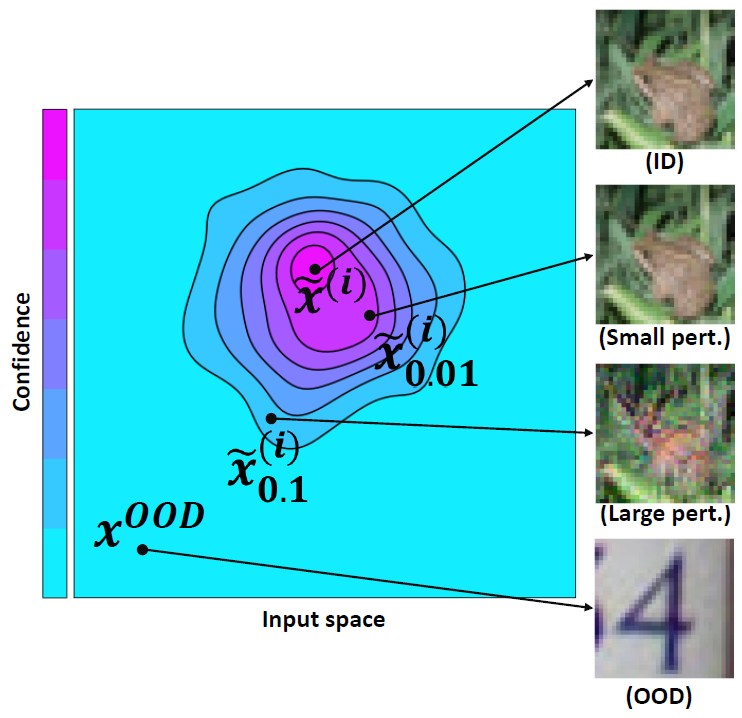
\includegraphics[width=0.36\textwidth]{sections/008_icml2021/eval/uncertainty_diagram.png}
\caption{Visualization of the desired uncertainty estimates. 
}
\label{fig:uncertainty_attack_diagram}
\end{figure}
%
DBU models have the advantage that they provide both, aleatoric uncertainty estimates resulting from irreducible uncertainty (e.g. class overlap or noise) and epistemic uncertainty estimates resulting from the lack of knowledge about unseen data (e.g. an unknown object is presented to the model). Both uncertainty types can be quantified from Dirichlet distributions using different uncertainty measures such as differential entropy, mutual information, or pseudo-counts. These uncertainty measures show outstanding performance in, e.g., the detection of OOD samples and thus are superior to softmax based confidence \citep{malini2018, reverse-kl, charpentier2020}.

Neural networks from the families outlined above are expected to \emph{know what they don't know}, i.e. they are supposed to notice when they are unsure about a prediction. 
This raises questions with regards to adversarial examples: should uncertainty estimation methods \emph{detect} these corrupted samples by indicating a high uncertainty on them and abstain from making a prediction? Or should uncertainty estimation be \emph{robust} to adversarial examples and assign the correct label even under perturbations? We argue that being robust to adversarial perturbations is the best option (see \cref{fig:uncertainty_attack_diagram}) for two reasons. First, in image classification a human is usually not able to observe any difference between an adversarial example and an unperturbed image. Second, the size of the perturbation corresponding to a good adversarial example is typically small w.r.t.\ the $L_p$-norm and thus assumed to be semantically meaningless. 
Importantly, robustness should not only be required for the class predictions, but also for the uncertainty estimates. This means that DBU models should be able to distinguish robustly between ID and OOD data even if those are perturbed. 
%Importantly, one should require robustness not only for the class predictions, but also for the uncertainty estimation. This means that DBU models should be able to distinguish robustly between ID and OOD data even if those are perturbed. 

In this chapter, we focus on DBU models and analyze their robustness capacity w.r.t. class predictions as well as uncertainty predictions. In doing so, we go beyond simple softmax output confidence by investigating advanced uncertainty measures such as differential entropy.
Specifically, we study the following questions: 
%
\begin{enumerate}
    \item \emph{Is low uncertainty a reliable indicator of correct predictions?}
    \item \emph{Can we use uncertainty estimates to detect label attacks on the class prediction?}
    \item \emph{Are uncertainty estimates such as differential entropy a robust feature for OOD detection?}
\end{enumerate}

In addressing these questions we place particular focus on adversarial perturbations of the input to evaluate the \emph{worst case} performance of the models on increasing complex data sets and attacks.
%
We evaluate robustness of DBU models w.r.t. to these three questions by comparing their performance on unperturbed and perturbed inputs. Perturbed inputs are obtained by computing \emph{label attacks} and \emph{uncertainty attacks}, which are a new type of attacks we propose.  While label attacks aim at changing the class prediction, uncertainty attacks aim at changing the uncertainty estimate such that ID data is marked as OOD data and vice versa.
%
In total, we performed more than $138,800$ attack settings to explore the robustness landscape of DBU models. Those settings cover different data sets, attack types, attack losses, attack radii, DBU model types and initialisation seeds.
%
Finally, we propose and evaluate median smoothing and adversarial training based on label attacks and uncertainty attacks to make DBU models more robust. Our median smoothing approach provides certificates on epistemic uncertainty measures such as differential entropy and allows to certify uncertainty estimation.  The code and further supplementary material is available online (\url{www.daml.in.tum.de/dbu-robustness}).





\section{Related Work}
\label{sec:related_work_010}

Predictions based on discrete sequences of events regardless of time can be modelled by Markov Models \cite{MarkovModel1} or RNNs, usually with its more advanced variants like LSTMs \cite{LSTM} and GRUs \cite{GRU}. To exploit the time information some models \cite{TimeDependentRNN, PhasedLstm} additionally take time as an input but still output a single prediction for the entire future. In contrast, temporal point process framework defines the intensity function that describes the rate of events occuring over time.

RMTPP \cite{RMTPP} uses an RNN to encode the event history into a vector that defines an exponential intensity function. Hence, it is able to capture complex past dependencies and model distributions resulting from simple point processes, such as Hawkes \cite{hawkes1971spectra} or self-correcting \cite{SelfCorrecting}, but not e.g.\ multimodal distributions. On the other hand, Neural Hawkes Process \cite{hawkes} uses continuous-time LSTM which allows specifying more complex intensity functions. Now the likelihood evaluation is not in closed-form anymore, but requires Monte Carlo integration. However, these approaches, unlike our models, do not provide any uncertainty in the predictions. In addition, \GPModel and \DirModel can be extended with a point process framework while having the expressive power to represent complex time evolutions.

% To allow modelling the event together with a time of occurrence, RMTPP \cite{RMTPP} and Neural Hawkes Process \cite{hawkes} combine RNNs with a point process framework to compute the intensities at each time point. \bc{Hence, RMTPP is able to model decaying intensities (like many other point processes, e.g. Cox, Hawkes) and Neural Hawkes Process is able to model multimodal distributions. However, these approaches do not provide any uncertainty in the predictions. Should we mention the expressive power of WGP-LN and FD-DIR to model complex time evolutions ?}

%However, these approaches do not focus on approximating multimodal distributions over time neither do they provide any uncertainty in the predictions.

Uncertainty in machine learning has shown a great interest \cite{BayesianRNN, PowerCertainty, Ensemble}. For example, uncertainty can be imposed by introducing distributions over the weights \cite{WeightUncertainty, BayesianRNNForecastingUncertainty, LaplaceNN}. Simpler approaches introduce uncertainty directly on the class prediction by using Dirichlet distribution independent of time \cite{PriorNetworks, NNRBetaDir}. In contrast, the \DirModel model models complex temporal evolution of Dirichlet distribution via function decomposition which can be adapted to have a point process interpretation.

Other methods introduce uncertainty time series prediction by learning state space model with Gaussian processes \cite{StateSpaceGPIdentification, StateSpaceGP}. Alternatively, RNN architecture has been used to model the probability density function over time \cite{ProbabilityEvolutionRNN}. Compared to these models, the \GPModel model uses both Gaussian processes and RNN to model uncertainty and time. Our models are based on pseudo points. Pseudo points in a GP have been used to reduce the computational complexity \cite{SparseGP}. Our goal is not to speed up the computation, since we control the number of points that are generated, but to give them different importance. In \cite{WeightedGP} a weighted GP has been considered by rescaling points; in contrast, our model uses a custom kernel to discard (pseudo) points.

\section{Dirichlet-based uncertainty models}
\label{sec:dirichlet_models}
%
Standard (softmax) neural networks predict the parameters of a categorical distribution \smash{$\vp\dataix = [p\dataix_1, \ldots, p\dataix_\nclass]$} for a given input \smash{$\x\dataix \in \mathbb{R}^{d}$}, where $\nclass$ is the number of classes. 
Given the parameters of a categorical distribution, the \emph{ aleatoric uncertainty} can be evaluated. The aleatoric uncertainty is the uncertainty on the class label prediction \smash{$y\dataix \in \{1, \ldots, \nclass\}$}. For example if we predict the outcome of an unbiased coin flip, the model is expected to have high aleatoric uncertainty and predict $p(\text{head})=0.5$.

\begin{table*}[ht]
	\centering
	\caption{Summary of DBU models. Further details on the loss functions are provided in the appendix.}
	\label{tab:dirichlet_models}
	\resizebox{.9 \textwidth}{!}{%
		\begin{tabular}{lllllll}
			\toprule
			{} &  \textbf{$\alpha\dataix$-parametrization} & \textbf{Loss} & \textbf{OOD training data} & \textbf{Ensemble training} & \textbf{Density estimation}\\
			\midrule
			\textbf{\PostNet} & $f_{\theta}(\x\dataix) = \mathbf{1} + \bm{\alpha}\dataix$ & Bayesian loss & No & No & Yes \\
			\textbf{\PriorNet} & $f_{\theta}(\x\dataix) = \bm{\alpha}\dataix$ & Reverse KL & Yes &  No & No \\
			\textbf{\DDNet} & $f_{\theta}(\x\dataix) = \bm{\alpha}\dataix$ & Dir. Likelihood & No & Yes & No \\
			\textbf{\EvNet} & $f_{\theta}(\x\dataix) =  \mathbf{1} + \bm{\alpha}\dataix$ & Expected MSE & No &  No & No \\
			\bottomrule
		\end{tabular}
	}
	%\vspace{-.5cm}
\end{table*}


In contrast to standard (softmax) neural networks, DBU models predict the parameters of a Dirichlet distribution -- the natural prior of categorical distributions -- given input~$\x \dataix$ (i.e. \smash{$q\dataix = \text{Dir}(\bm{\alpha}\dataix)$} where \smash{$f_{\theta}(\x\dataix) = \bm{\alpha} \dataix \in \mathbb{R}_+^\nclass$}). Hence, the \emph{epistemic distribution} \smash{$q\dataix$} expresses the \emph{epistemic} uncertainty on $\x \dataix$, i.e. the uncertainty on the categorical distribution prediction \smash{$\vp\dataix$}. From the epistemic distribution, follows an estimate of the \emph{aleatoric distribution} of the class label prediction $\text{Cat}(\bar{\vp}\dataix)$ where \smash{$\E_{q\dataix}[\vp\dataix] = \bar{\vp}\dataix$}.
An advantage of DBU models is that one pass through the neural network is sufficient to compute epistemic distribution, aleatoric distribution, and predict the class label:
%
\begin{equation}
\begin{aligned}
    q^{(\idata)}           = \text{Dir}(\bm{\alpha}\dataix), \hspace{5pt}
    \bar{p}_\iclass\dataix  = \frac{\alpha_\iclass\dataix}{\alpha_0\dataix}, \hspace{5pt}
    y^{(\idata)}           = \arg \max_{\iclass} \;[\bar{p}_\iclass\dataix]
\end{aligned}
\end{equation}
%
where $\alpha_0\dataix = \sum^{\nclass}_{\iclass=1} \alpha_\iclass\dataix$. This parametrization allows to compute classic uncertainty measures in closed-form such as the total pseudo-count $m\dataix_{\alpha_0} = \sum_\iclass \alpha\dataix_\iclass$, the differential entropy of the Dirichlet distribution $m\dataix_\text{diffE} = h(\text{Dir}(\bm{\alpha}\dataix))$ or the mutual information $m\dataix_\text{MI} = I(y\dataix, \vp\dataix)$ (App. \ref{subsec:appendix_measurecomp}, \citep{malini2018}). 
Hence, these measure can efficiently be used to assign high uncertainty to unknown data, which makes DBU models specifically suited for detection of OOD samples. 





Several recently proposed models for uncertainty estimations belong to the family of DBU models, such as \PriorNet, \EvNet, \DDNet and \PostNet. These models differ in terms of their parametrization of the Dirichlet distribution, the training, and density estimation. An overview of theses differences is provided in Table \ref{tab:dirichlet_models}. In our study we evaluate all recent versions of these models.


Contrary to the other models, Prior Networks \textbf{(\PriorNet)} \citep{malini2018, malinin2019}  require OOD data for training to ``teach'' the neural network the difference between ID and OOD data. \PriorNet is trained with a loss function consisting of two KL-divergence terms. The fist term is designed to learn Dirichlet parameters for ID data, while the second one is used to learn a flat Dirichlet distribution %($\boldsymbol{\alpha} = \boldsymbol{1}$) 
for OOD data: 
%
\begin{equation}
\begin{aligned}
    L_{\mathrm{\PriorNet}} &= \frac{1}{N} \left[\sum_{\x\dataix \in \text{ID data}}  [\mathrm{KL} [\mathrm{Dir} (\alpha^{\mathrm{ID}}) || q\dataix]]  \right. \\
                           &+ \left.\sum_{\x\dataix \in OOD data} [\mathrm{KL} [\mathrm{Dir} (\alpha^{\mathrm{OOD}}) || q\dataix]]\right] \\
\end{aligned}
\end{equation}
%
where $\alpha^{\mathrm{ID}}$ and $\alpha^{\mathrm{OOD}}$ are hyper-parameters. Usually $\alpha^{\mathrm{ID}}$ is set to $1e^{1}$ for the correct class and $1$ for all other classes, while $\alpha^{\mathrm{OOD}}$ is set to $\mathbf{1}$ for all classes.
%
There a two variants of \PriorNet. The first one is trained based on reverse KL-divergence \citep{malinin2019}, while the second one is trained with KL-divergence \citep{malini2018}. In our experiments, we include the most recent reverse version of \PriorNet, as it shows superior performance \citep{malinin2019}. 

Evidential Networks \textbf{(\EvNet)} \citep{sensoy2018} are trained with a loss that computes the sum of squares between the on-hot encoded true label $\vy*\dataix$ and the predicted categorical $\vp\dataix$ under the Dirichlet distribution:
%
\begin{equation}
\begin{aligned}
    L_{\mathrm{\EvNet}} &= \frac{1}{N} \sum_i \E_{\vp\dataix \sim \text{Dir}(\bm{\alpha}\dataix)}||\vy*\dataix - \vp\dataix||^2 \\
\end{aligned}
\end{equation}

Ensemble Distribution Distillation \textbf{(\DDNet)} \citep{malinin2019ensemble} is trained in two steps. First, an ensemble of $M$ classic neural networks needs to be trained. 
Then, the soft-labels \smash{$\{\vp_{m}\dataix\}_{m=1}^{M}$} provided by the ensemble of networks are distilled into a Dirichlet-based network by fitting them with the maximum likelihood under the Dirichlet distribution: 
\begin{equation}
\begin{aligned}
    L_{\mathrm{\DDNet}} &= - \frac{1}{N}  \sum_i \sum_{m=1}^{M} [\ln q\dataix(\pi^{im})] \\
\end{aligned}
\end{equation}
where $\pi^{im}$ denotes the soft-label of $m$th neural network. 

Posterior Network \textbf{(\PostNet)} \citep{charpentier2020} performs density estimation for ID data with normalizing flows and uses a Bayesian loss formulation: %composed of the Uncertain Cross-Entropy loss \citep{uncertainty_time} and an entropy regularizer inspired by Bayesian theory.
\begin{equation}
\begin{aligned}
    L_{\mathrm{\PostNet}} &= \frac{1}{N} \sum_i \E_{q(p\dataix)}  [\mathrm{CE} (p\dataix, y\dataix)] - H(q\dataix)
\end{aligned}
\end{equation}
where $\mathrm{CE}$ denotes the cross-entropy.
%
All loss functions can be computed in closed-form. For more details please have a look at the original paper on \PriorNet \citep{malini2018}, \PostNet \citep{charpentier2020}, \DDNet \citep{malinin2019} and \EvNet \citep{sensoy2018}.
Note that \EvNet and \PostNet model the Dirichlet parameters as \smash{$f_{\theta}(\x\dataix) = 1 + \bm{\alpha}\dataix$} while \PriorNet, \RevPriorNet and \DDNet compute them as \smash{$f_{\theta}(\x\dataix) = \bm{\alpha}\dataix$}. 









\section{Robustness of Dirichlet-based uncertainty models}
\label{sec:attack_dirichlet_model}

We analyze robustness of DBU models on tasks in connection with uncertainty estimation w.r.t.\ the following four aspects: \emph{accuracy}, \emph{confidence calibration}, \emph{label attack detection} and \emph{OOD detection}. Uncertainty is quantified by differential entropy, mutual information or pseudo counts. 
A formal definition of all uncertainty estimation measures is provided in the appendix (see Section~\ref{subsec:appendix_measurecomp}).  

Robustness of Dirichlet-based uncertainty models is evaluated based on \emph{label attacks} and a newly proposed type of attacks called \emph{uncertainty attacks}. 
While label attacks aim at changing the predicted class, uncertainty attacks aim at changing the uncertainty assigned to a prediction. 
All previous works are based on label attacks and focus on robustness w.r.t. the class prediction. Thus, we are the first to propose attacks targeting uncertainty estimates such as differential entropy and analyze desirable robustness properties of DBU models beyond the class prediction. 
Label attacks and uncertainty attacks both compute a perturbed input $\tilde{\x}\dataix$ close to the original input~$\x\dataix$ i.e. $|| \x\dataix - \tilde{\x}\dataix ||_2 < r$ where $r$ is the attack radius. This perturbed input is obtained by optimizing a loss function $l(\x)$ using Fast Gradient Sign Method (FGSM) or Projected Gradient Descent (PGD). Furthermore, we include a black box attack setting (Noise) which generates 10 noise samples from a Gaussian distribution, which is centered at the original input. From these 10 perturbed samples we choose the one with the greatest effect on the loss function and use it as attack. 
To complement attacks, we compute certificates on uncertainty estimates using median smoothing \cite{median_smoothing}. 


%Reviewer: avoid redundancy within assessment metric paragraphs, explain high level + differences
The following questions we address by our experiments have a common assessment metric and can be treated as binary classification problems: distinguishing between correctly and wrongly classified samples, discriminating between non-attacked input and attacked inputs or differentiating between ID data and OOD data. To quantify the performance of the models on these binary classification problems, we compute the area under the precision recall curve (AUC-PR).

Experiments are performed on two image data sets (MNIST \citep{mnist} and CIFAR10 \citep{cifar10}), which contain bounded inputs and two tabular data sets (Segment \citep{uci_datasets} and Sensorless drive \citep{uci_datasets}), consisting of unbounded inputs. Note that unbounded inputs are challenging since it is impossible to describe the infinitely large OOD distribution. As PriorNet requires OOD training data, we use two further image data sets (FashionMNIST \citep{fashionmnist} and CIFAR100 \citep{cifar10}) for training on MNIST and CIFAR10, respectively. All other models are trained without OOD data. To obtain OOD data for the tabular data sets, we remove classes from the ID data set (class window for the Segment data set and class 9 for Sensorless drive) and use them as the OOD data. Further details on the experimental setup are provided in the appendix (see Section~\ref{subsec:exp_setup}).



 


\subsection{Uncertainty estimation under label attacks}
\label{subsec:label_attacks}
%
Label attacks aim at changing the predicted class. To obtain a perturbed input with a different label, we maximize the cross-entropy loss $\tilde{\x}\dataix \approx \arg\max_{\x} l(\x) = \text{CE}(\vp\dataix, \vy\dataix)$ under the radius constraint. For the sake of completeness we additionally analyze label attacks w.r.t. to their performance of changing the class prediction and the accuracy of the neural network under label attacks constraint by different radii (see Appendix, Table~\ref{tab:acc_label_attack}). As expected and partially shown by previous works, none of the DBU models is robust against label attacks. %, neither on the image data sets nor on the tabular data sets.
However, we note that \PriorNet is slightly more robust than the other DBU models. This might be explained by the use of OOD data during training, which can be seen as some kind of robust training. 
%
From now on, we switch to the core focus of this work and analyze robustness properties of uncertainty estimation. 




\begin{table*}[ht]
	\centering
	\caption{Distinguishing between correctly predicted and wrongly predicted labels based on the differential entropy under PGD label attacks (metric: AUC-PR).}
	%\begin{small}
	\resizebox{0.8\textwidth}{!}{
		\begin{tabular}{@{}rrrrrrrc|crrrrrr@{}}
			\toprule
			& \multicolumn{6}{c}{CIFAR10} & & & \multicolumn{6}{c}{Sensorless} \\
			\cmidrule{2-7}  \cmidrule{10-15}
			Att. Rad. & 0.0 & 0.1 & 0.2 & 0.5 & 1.0 & 2.0 & & & 0.0 & 0.1 & 0.2 & 0.5 & 1.0 & 2.0  \\
			\midrule
			%& \multicolumn{7}{c}{MNIST} & & & \multicolumn{7}{c}{CIFAR10} \\
			\PostNet  &  \bf{98.7} &  88.6 &  56.2 &   7.8 &   1.2 &   0.4 &  & %0.3 & & 
			&  99.7 &   8.3 &   3.9 &  3.6 &  \bf{7.0} &  \bf{9.8} \\%&  \bf{11.3} \\
			\PriorNet &  92.9 &  77.7 &  60.5 &  \bf{37.6} &  \bf{24.9} &  \bf{11.3} &  & %\bf{3.0} & & 
			&  99.8 &  10.5 &   3.2 &  0.7 &  0.2 &  0.2 \\%&   2.2 \\ 
			\DDNet    &  97.6 &  \bf{91.8} &  \bf{78.3} &  18.1 &   0.8 &   0.0 &  &%0.0 & &
			&  99.7 &  11.9 &   1.6 &  0.4 &  0.2 &  0.1 \\%&   0.2 \\ 
			\EvNet    &  97.9 &  85.9 &  57.2 &  10.2 &   4.0 &   2.4 &  &%0.3 & & 
			&  \bf{99.9} &  \bf{22.9} &  \bf{13.0} &  \bf{6.0} &  3.7 &  3.2 \\%&   3.1 \\
			\bottomrule
		\end{tabular}}
	%\end{small}
	\label{tab:conf_label_attack}
\end{table*}







\textbf{Is low uncertainty a reliable indicator of correct predictions?} \\
%
\underline{\emph{Expected behavior:}}  Predictions with low uncertainty are more likely to be correct than high uncertainty predictions. 
\underline{\emph{Assessment metric:}} We distinguish between correctly classified samples (label 0) and wrongly classified ones (label 1) based on the differential entropy scores produced by the DBU models \citep{malini2018}. Correctly classified samples are expected to have low differential entropy, reflecting the model's confidence, and analogously wrongly predicted samples are expected to have higher differential entropy. 
%\dz{State that the metric is AUC-PR?} 
\underline{\emph{Observed behavior:}} Note that the positive and negative class are not balanced, thus, the use of AUC-PR scores \citep{imbalance_apr} are important to enable meaningful measures. While uncertainty estimates are indeed an indicator of correctly classified samples on unperturbed data, none of the models maintains its high performance on perturbed data computed by PGD, FGSM or Noise label attacks (see. Table~\ref{tab:conf_label_attack}, \ref{tab:conf_label_attack_fgsm} and \ref{tab:conf_label_attack_noise_attack}). Thus, using uncertainty estimates as indicator for correctly labeled inputs is not robust to adversarial perturbations. This result is notable, since the used attacks do not target uncertainty. 





\vspace{1em}
\begin{table*}[ht]
	\centering
	\caption{Label Attack-Detection by normally trained DBU models based on differential entropy under PGD label attacks (AUC-PR).}
	%\begin{small}
	\resizebox{0.8\textwidth}{!}{
		\begin{tabular}{@{}rrrrrrc|crrrrr@{}}
			\toprule
			& \multicolumn{5}{c}{CIFAR10} & & & \multicolumn{5}{c}{Sensorless} \\
			\cmidrule{2-6}  \cmidrule{9-13}
			Att. Rad. & 0.1 & 0.2 & 0.5 & 1.0 & 2.0 & & & 0.1 & 0.2 & 0.5 & 1.0 & 2.0 \\
			\midrule
			\PostNet  &  \bf{63.4} &  \bf{66.9} &  42.1 &  32.9 &  31.6 &  &%31.2 & & 
			&  47.7 &  42.3 &  36.9 &  \bf{48.5} &  \bf{85.0} \\%&  \bf{99.0} \\ 
			\PriorNet &  53.3 &  56.0 &  55.6 &  \bf{49.2} &  42.2 & &%  35.4 & & 
			&  38.8 &  33.6 &  31.4 &  33.1 &  40.9 \\%&  53.5 \\ 
			\DDNet    &  55.8 &  60.5 &  \bf{57.3} &  38.7 &  32.3 & &% 31.4 & & 
			&  \bf{53.5} &  42.2 &  35.0 &  32.8 &  32.6 \\%&  33.9 \\ 
			\EvNet    &  48.4 &  46.9 &  46.3 &  46.3 &  \bf{44.5} & &% \bf{42.5} & &
			&  48.2 &  \bf{42.6} &  \bf{38.2} &  36.0 &  37.2 \\%&  41.7 \\
			\bottomrule 			
		\end{tabular}}
	%\end{small}
	\label{tab:label_attack_detect}
\end{table*}








%\vspace{-0.5em}
\textbf{Can uncertainty estimates be used to detect label attacks against the class prediction?}\\
%
\underline{\emph{Expected behavior:}} Adversarial examples are not from the natural data distribution. Therefore, DBU models are expected to detect them as OOD data by assigning them a higher uncertainty. We expect that perturbations computed based on a bigger attack radius~$r$ are easier to detect as their distance from the data distribution is larger. 
\underline{\emph{Assessment metric:}} The goal of attack-detection is to distinguish between unperturbed samples (label 0) and perturbed samples (label 1). Uncertainty on samples is quantified by the differential uncertainty \citep{malini2018}. Unperturbed samples are expected to have low differential entropy, because they are from the same distribution as the training data, while perturbed samples are expected to have a high differential entropy. 
%Further results based on other uncertainty measures are provided in the appendix. 
\underline{\emph{Observed behavior:}} Table~\ref{tab:acc_label_attack} shows that the accuracy of all models decreases significantly under PGD label attacks, but none of the models is able to provide an equivalently increasing attack detection rate (see Table~\ref{tab:label_attack_detect}). Even larger perturbations are hard to detect for DBU models. 

Similar results are obtained when we use mutual information or the precision~$\alpha_0$ to quantify uncertainty (see appendix Table~\ref{tab:conf_label_attack_mi} and~\ref{tab:conf_label_attack_alpha}).
Although PGD label attacks do not explicitly consider uncertainty, they seem to generate adversarial examples with similar uncertainty as the original input. 
Such high-certainty adversarial examples are illustrated in Figure~\ref{fig:attaked_samples_labels}, where certainty is visualized based on the precision~$\alpha_0$, which is supposed to be high for ID data and low for OOD data. While the original input (perturbation size $0.0$) is correctly classified as frog and ID data, there exist adversarial examples that are classified as deer or bird. The certainty ($\alpha_0$-score) on the prediction of these adversarial examples has a similar or even higher value than on the prediction of the original input. Using the differential entropy to distinguish between ID and OOD data results in the same ID/OOD assignment since the differential entropy of the three right-most adversarial examples is similar or even smaller than on the unperturbed input. 







Under the less powerful FGSM and Noise attacks (see Appendix), DBU models achieve mostly higher attack detection rates than under PGD attacks. This suggests that uncertainty estimation is able to detect weak attacks, which is consistent with the observations in \citep{malinin2018_adetect} but fails under stronger PGD attacks. 
%
\begin{figure}[ht]
	\centering
	\resizebox{0.42\textwidth}{!}{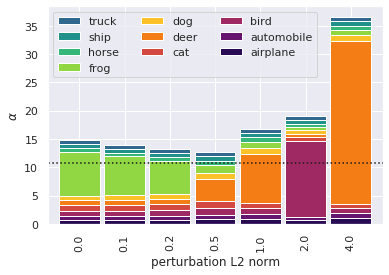
\includegraphics[width=\textwidth]{sections/008_icml2021/eval/ddnet_label_id_cifar10_alphas.png}}%
	\resizebox{0.42\textwidth}{!}{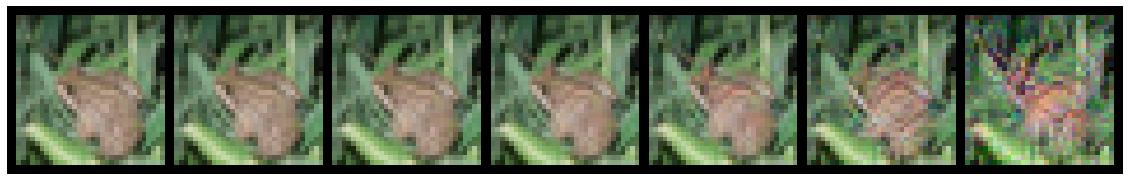
\includegraphics[width=\textwidth]{sections/008_icml2021/eval/ddnet_label_id_cifar10_images.png}}
	\caption{Input and predicted Dirichlet-parameters under label attacks (dotted line: threshold to distinguish ID and OOD data). % based on the precision~$\alpha_0$.
		%-14.2216765174
		%0.0 [-17.875761]
		%0.1 [-17.257824]
		%0.2 [-16.648003]
		%0.5 [-15.014889]
		%1.0 [-17.504786]
		%2.0 [-22.63896]
		%4.0 [-24.941536]
	}
	\label{fig:attaked_samples_labels}
\end{figure}


On tabular data sets, \PostNet shows a better label attack detection rate for large perturbations. This observation might be explained by the fact that the density estimation of the ID samples has been shown to work better for tabular data sets \citep{charpentier2020}. 
%
Overall, none of the DBU models provides a reliable indicator for adversarial inputs that target the class prediction. 





\vspace{.4mm}
\begin{table*}[ht]
	\centering
	\caption{OOD detection based on differential entropy under PGD uncertainty attacks against differential entropy computed on ID data and OOD data (metric: AUC-PR).}
%	\begin{small}
	\resizebox{\textwidth}{!}{
		\begin{tabular}{@{}rrrrrrrc|crrrrrr@{}}
			\toprule
			& \multicolumn{6}{c}{ID-Attack (non-attacked OOD)} &  & &  \multicolumn{6}{c}{OOD-Attack (non-attacked ID)} \\
			\cmidrule{2-7}  \cmidrule{10-15}
			Att. Rad. & 0.0 & 0.1 & 0.2 & 0.5 & 1.0 & 2.0 & & &
			0.0 & 0.1 & 0.2 & 0.5 & 1.0 & 2.0  \\
			\midrule
			& \multicolumn{14}{c}{\textbf{CIFAR10 -- SVHN}} \\
			\PostNet  &  81.8 &  64.3 &  47.2 &  22.4 &  17.6 &  \bf{16.9} &  &%\bf{16.4} & &
			&  81.8 &  60.5 &  40.7 &  23.3 &  21.8 &  19.8 \\%&  18.1 \\ 
			\PriorNet &  54.4 &  40.1 &  30.0 &  17.9 &  15.6 &  15.4 &  &%15.4 & &
			&  54.4 &  40.7 &  30.7 &  19.5 &  16.5 &  15.7 \\%&  15.4 \\
			\DDNet    &  \bf{82.8} &  \bf{71.4} &  \bf{59.2} &  \bf{28.9} &  16.0 &  15.4 & &% 15.4 & &
			&  \bf{82.8} &  \bf{72.0} &  \bf{57.2} &  20.8 &  15.6 &  15.4 \\%&  15.4 \\
			\EvNet    &  80.3 &  62.4 &  45.4 &  21.7 &  \bf{17.9} &  16.5 &  &%15.6 & &
			&  80.3 &  58.2 &  46.5 &  \bf{34.6} &  \bf{28.0} &  \bf{23.9} \\%&  \bf{21.0} \\
			\midrule
			& \multicolumn{14}{c}{\textbf{Sens. -- Sens. class 10, 11}} \\
			\PostNet  &  \bf{74.5} &  \bf{39.8} &  \bf{36.1} &  \bf{36.0} &  \bf{45.9} &  \bf{46.0} & &% \bf{46.0} & &
			&  \bf{74.5} &  \bf{43.3} &  \bf{42.0} &  \bf{32.1} &  \bf{35.1} &  \bf{82.6} \\%&  \bf{99.4} \\
			\PriorNet &  32.3 &  26.6 &  26.5 &  26.5 &  26.6 &  28.3 & &% 38.6 & &
			&  32.3 &  26.7 &  26.6 &  26.6 &  27.0 &  30.4 \\%&  36.8 \\ 
			\DDNet    &  31.7 &  26.8 &  26.6 &  26.5 &  26.6 &  27.1 & &% 30.5 & &
			&  31.7 &  27.1 &  26.7 &  26.7 &  26.8 &  26.9 \\%&  27.3 \\ 
			\EvNet    &  66.5 &  30.5 &  28.2 &  27.1 &  28.1 &  31.8 & &% 37.5 & &
			&  66.5 &  38.7 &  36.1 &  30.2 &  28.2 &  28.8 \\%&  32.2 \\
			\bottomrule
		\end{tabular}}
%	\end{small}
	\label{tab:id_ood_attacks}
\end{table*}









\subsection{Attacking uncertainty estimation}
\label{subsec:uncertainty_attacks}

DBU models are designed to provide sophisticated uncertainty estimates (beyond softmax scores) alongside predictions and use them to detect OOD samples. In this section, we propose and analyze a new attack type that targets these uncertainty estimates. 
DBU models enable us to compute uncertainty measures i.e. differential entropy, mutual information and precision~$\alpha_0$ in closed from (see \citep{malini2018} for a derivation). Uncertainty attacks use this closed form solution as loss function for PGD, FGSM or Noise attacks. 
Since differential entropy is the most widely used metric for ID-OOD-differentiation, we present results based on the differential entropy loss function $\tilde{\x}\dataix \approx \arg\max_{\x} l(\x) = \text{Diff-E}(\text{Dir}(\mathbf{\alpha}\dataix))$: 
%
\begin{equation}
\begin{aligned}
	\text{Diff-E}(\text{Dir}(\mathbf{\alpha}\dataix))  = &\sum_c^K \ln \Gamma (\alpha_c^{(i)}) - \ln \Gamma (\alpha_0^{(i)}) \\
	&- \sum_c^K (\alpha_c^{(i)} -1) \cdot (\Psi (\alpha_c^{(i)}) - \Psi (\alpha_0^{(i)}))
\end{aligned}
\end{equation}
%
where $\alpha_0^{(i)} = \sum_c \alpha_c^{(i)}$. 
Result based on further uncertainty measures, loss functions and more details on attacks are provided in the appendix. 


We analyze the performance of DBU models under uncertainty attacks w.r.t.\ two tasks. First, uncertainty attacks are computed on ID data aiming to indicate it as OOD data, while OOD data is left non-attacked. Second, we attack OOD data aiming to indicate it as ID data, while ID data is not attacked. Hence, uncertainty attacks target at posing ID data as OOD data and vice versa.


\begin{figure}[ht!]
    \centering
        \begin{subfigure}[t]{0.49\columnwidth}
        \centering
        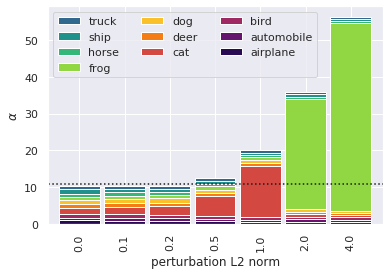
\includegraphics[width=0.99 \textwidth]{sections/008_icml2021/eval/ddnet_unc_ood_cifar10_alphas.png}
    \end{subfigure}%
    \begin{subfigure}[t]{0.49\columnwidth}
        \centering
        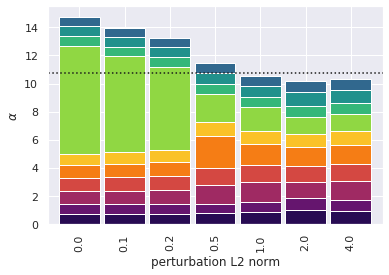
\includegraphics[width=0.99 \textwidth]{sections/008_icml2021/eval/ddnet_unc_id_cifar10_alphas.png}
    \end{subfigure}%


    \begin{subfigure}[t]{0.49 \columnwidth}
        \centering
        
\includegraphics[width=0.99 \textwidth]{sections/008_icml2021/eval/ddnet_unc_ood_cifar10_images.png}
        \caption{OOD uncertainty attack
        %-14.2216765174
        %0.0 [-13.115507]
        %0.1 [-13.353642]
        %0.2 [-13.723262]
        %0.5 [-16.341246]
        %1.0 [-22.298155]
        %2.0 [-28.071136]
        %4.0 [-33.148224]
        }
        \label{fig:attaked_samples_idood_a}
    \end{subfigure}%
        \begin{subfigure}[t]{0.49 \columnwidth}
        \centering
        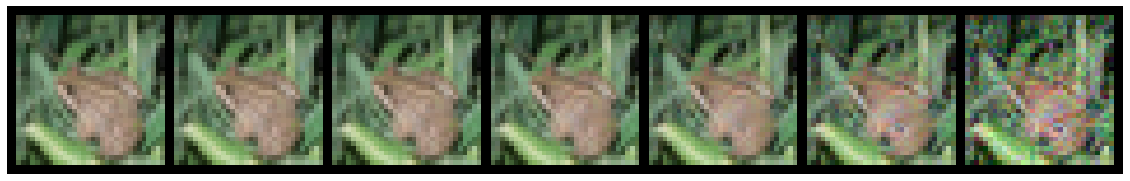
\includegraphics[width=0.99 \textwidth]{sections/008_icml2021/eval/ddnet_unc_id_cifar10_images.png}
        \caption{ID uncertainty attack
        %-14.2216765174
        %0.0 [-17.875761]
        %0.1 [-17.256058]
        %0.2 [-16.65203]
        %0.5 [-14.321844]
        %1.0 [-13.6354265]
        %2.0 [-13.046129]
        %4.0 [-13.1426115]
        }
        \label{fig:attaked_samples_idood_b}
    \end{subfigure}%
    \caption{ID and OOD input with corresponding Dirichlet-parameters under uncertainty attacks (dotted line: threshold to distinguish ID and OOD).}
    \label{fig:attaked_samples_idood}
	%\vspace{-.5cm}
\end{figure}





\textbf{Are uncertainty estimates a robust feature for OOD detection?}\\
%
\underline{\emph{Expected behavior:}} We expect DBU models to be able to distinguish between ID and OOD data by providing reliable uncertainty estimates, even under small perturbations. Thus, we expect uncertainty estimates of DBU models to be robust under attacks. 
%
\underline{\emph{Assessment metric:}} We distinguish between ID data (label 0) and OOD data (label 1) based on the differential entropy as uncertainty scoring function \citep{malini2018}. Differential entropy is expected to be small on ID samples and high on OOD samples. Experiments on further uncertainty measure and results on the AUROC metric are provided in the appendix. 
%
\underline{\emph{Observed behavior:}} OOD samples are perturbed as illustrated in  Figure~\ref{fig:attaked_samples_idood}. Part (a) of the figure illustrates an OOD-samples, that is correctly identified as OOD. Adding adversarial perturbations $\geq 0.5$ changes the Dirichlet parameters such that the resulting images are identified as ID, based on precision or differential entropy as uncertainty measure. Perturbing an ID sample (part (b)) results in images that are marked as OOD samples. 
OOD detection performance of all DBU models rapidly decreases with the size of the perturbation, regardless of whether attacks are computed on ID or OOD data (see Table~\ref{tab:id_ood_attacks}). This performance decrease is also observed with AUROC as metric, attacks based on FGSM, Noise, when we use mutual information or precision~$\alpha_0$ to distinguish between ID samples and OOD samples (see appendix Table~\ref{tab:id_ood_attacks_part2} - \ref{tab:id_ood_attacks_measure_diffE_aupr_noise}). 
Thus, using uncertainty estimation to distinguish between ID and OOD data is not robust. 








\begin{table*}[ht!]
	\centering
	%\begin{tiny}
	\resizebox{\textwidth}{!}{ %0.866
%    \begin{tabular}{lccccccc}
%    \toprule
 %   \textbf{Att. Rad.} & 0.0 &   0.1 &  0.2 &  0.5 &  1.0 &  2.0 \\
 %   \midrule
  %  & \multicolumn{6}{c}{\textbf{Smoothed models}} \\
%    \input{tables_v2/normal-cifar10-in-PGD_L2-crossentropy-confidence}
%    \midrule
%    & \multicolumn{6}{c}{\textbf{Smoothed models + adversarial training using label attacks}} \\
%    \input{tables_v2/adv-cifar10-in-PGD_L2-crossentropy-confidence}
%    \midrule
%    & \multicolumn{6}{c}{\textbf{Smoothed models + adversarial training using uncertainty attacks}} \\
%    \input{tables_v2/unc_adv-cifar10-in-PGD_L2-crossentropy-confidence}
%    \bottomrule
%    \end{tabular}
    \begin{tabular}{clccccccc}
    \toprule
    & \textbf{Att. Rad.} & 0.0 &   0.1 &  0.2 &  0.5 &  1.0 &  2.0 \\
    \midrule
    %& & \multicolumn{6}{c}{\textbf{Smoothed models}} \\
      \multirow{4}{1.2cm}{Smoothed models} & \textbf{PostNet} &  $80.5\cdot\bm{{\color{black}91.5}}\cdot94.5$ &  
  $52.8\cdot\bm{{\color{black}71.6}}\cdot95.2$ &  
  $31.9\cdot\bm{{\color{black}51.0}}\cdot96.8$ &  
  $\phantom{0}5.6\cdot\bm{{\color{blue}11.7}}\cdot100.0$ &  
  $\phantom{0}0.3\cdot\bm{{\color{black}\phantom{0}0.6}}\cdot100.0$ &  
  $\phantom{0}0.0\cdot\bm{{\color{black}\phantom{0}0.0}}\cdot100.0$ \\
 & \textbf{PriorNet} &  
 $81.9\cdot\bm{{\color{black}86.8}}\cdot88.0$ &     
 $69.6\cdot\bm{{\color{blue}78.0}}\cdot90.1$ &     
 $50.9\cdot\bm{{\color{blue}65.8}}\cdot89.4$ & 
 $36.5\cdot\bm{{\color{blue}59.9}}\cdot\phantom{0}97.0$ &   
 $24.3\cdot\bm{{\color{blue}39.3}}\cdot100.0$ &    
 $\phantom{0}9.2\cdot\bm{{\color{blue}17.9}}\cdot100.0$ \\
  &   \textbf{DDNet} &  
  $65.9\cdot\bm{{\color{black}81.2}}\cdot83.0$ &  
  $55.8\cdot\bm{{\color{black}70.5}}\cdot87.2$ &  
  $37.8\cdot\bm{{\color{black}56.8}}\cdot88.1$ &  
  $10.1\cdot\bm{{\color{blue}21.9}}\cdot\phantom{0}94.3$ &      
  $\phantom{0}0.9\cdot\phantom{0}\bm{{\color{blue}1.6}}\cdot\phantom{0}99.6$ &                   
  $\phantom{0}0.0\cdot\phantom{0}\bm{0.0}\cdot100.0$ \\
  &   \textbf{EvNet} &  
  $76.3\cdot\bm{{\color{black}90.2}}\cdot91.7$ &  
  $54.7\cdot\bm{{\color{black}74.3}}\cdot95.7$ &  
  $31.6\cdot\bm{{\color{black}51.5}}\cdot94.5$ &   
  $\phantom{0}5.8\cdot\bm{{\color{blue}11.9}}\cdot\phantom{0}86.9$ &     
  $\phantom{0}1.9\cdot\bm{{\color{blue}\phantom{0}7.0}}\cdot100.0$ &     
  $\phantom{0}1.1\cdot\bm{{\color{blue}\phantom{0}4.0}}\cdot100.0$ \\

    \midrule
    %& & \multicolumn{6}{c}{\textbf{Smoothed models + adversarial training using label attacks}} \\
      \multirow{4}{1.2cm}{Smoothed + adv. w. label attacks} &  
  \textbf{PostNet} &  - &  
  $52.1\cdot\bm{{\color{black}71.8}}\cdot95.6$ &  
  $31.2\cdot\bm{{\color{black}47.9}}\cdot96.1$ &  
  $\phantom{0}7.8\cdot\bm{{\color{blue}14.7}}\cdot\phantom{0}98.6$ &    
  $\phantom{0}1.8\cdot\phantom{0}\bm{{\color{blue}4.4}}\cdot100.0$ &  
  $\phantom{0}0.3\cdot\phantom{0}\bm{{\color{black}0.5}}\cdot100.0$ \\
 & \textbf{PriorNet} &  - &  
 $57.6\cdot\bm{{\color{black}71.7}}\cdot88.9$ &     
 $46.1\cdot\bm{{\color{blue}64.5}}\cdot90.1$ &  
 $38.1\cdot\bm{{\color{blue}59.3}}\cdot\phantom{0}99.5$ &  
 $32.3\cdot\bm{{\color{blue}51.7}}\cdot100.0$ &    
 $22.1\cdot\bm{{\color{blue}41.6}}\cdot\phantom{0}97.4$ \\
   & \textbf{DDNet} &  - &  
   $58.6\cdot\bm{{\color{black}78.4}}\cdot92.2$ &  
   $49.4\cdot\bm{{\color{black}66.0}}\cdot90.5$ &  
   $12.0\cdot\bm{{\color{blue}21.4}}\cdot\phantom{0}98.1$ &     
   $\phantom{0}0.8\cdot\phantom{0}\bm{{\color{blue}1.0}}\cdot\phantom{0}96.6$ &                   
   $\phantom{0}0.0\cdot\phantom{0}\bm{0.0}\cdot100.0$ \\
    & \textbf{EvNet} &  - &  
    $24.3\cdot\bm{{\color{black}34.2}}\cdot51.8$ &  
    $32.6\cdot\bm{{\color{black}49.5}}\cdot95.5$ &  
    $\phantom{0}5.9\cdot\bm{{\color{blue}13.0}}\cdot100.0$ &  
    $\phantom{0}2.6\cdot\phantom{0}\bm{{\color{black}5.2}}\cdot\phantom{0}99.9$ &     
    $\phantom{0}2.9\cdot\phantom{0}\bm{{\color{blue}5.9}}\cdot100.0$ \\

    \midrule
    %& & \multicolumn{6}{c}{\textbf{Smoothed models + adversarial training using uncertainty attacks}} \\
    \multirow{4}{1.3cm}{Smoothed + adv. uncert. attacks} &   
\textbf{PostNet} &  - &  
$52.8\cdot\bm{{\color{black}74.2}}\cdot94.6$ &  
$33.0\cdot\bm{{\color{black}49.4}}\cdot87.5$ &   
$\phantom{0}7.7\cdot\bm{{\color{blue}14.2}}\cdot\phantom{0}99.0$ &  
$\phantom{0}0.6\cdot\phantom{0}\bm{{\color{black}1.2}}\cdot100.0$ &    
$\phantom{0}0.7\cdot\phantom{0}\bm{{\color{blue}1.1}}\cdot100.0$ \\
 & \textbf{PriorNet} &  - &  
 $50.6\cdot\bm{{\color{black}68.1}}\cdot88.6$ &     
 $44.4\cdot\bm{{\color{blue}66.1}}\cdot96.0$ &  
 $35.1\cdot\bm{{\color{blue}57.4}}\cdot\phantom{0}98.4$ &   
 $18.4\cdot\bm{{\color{blue}32.2}}\cdot100.0$ &  
 $15.2\cdot\bm{{\color{blue}29.3}}\cdot100.0$ \\
   & \textbf{DDNet} &  - &  
   $68.8\cdot\bm{{\color{black}84.4}}\cdot93.2$ &  
   $45.1\cdot\bm{{\color{black}60.8}}\cdot86.8$ &  
   $12.3\cdot\bm{{\color{blue}22.0}}\cdot\phantom{0}91.0$ &      
   $\phantom{0}0.8\cdot\phantom{0}\bm{{\color{blue}1.7}}\cdot\phantom{0}87.0$ &                  
   $\phantom{0}0.0\cdot\phantom{0}\bm{0.0}\cdot100.0$ \\
&    \textbf{EvNet} &  - &  
$54.2\cdot\bm{{\color{black}73.7}}\cdot96.1$ &  
$30.5\cdot\bm{{\color{black}50.0}}\cdot99.5$ &  
$\phantom{0}7.1\cdot\bm{{\color{blue}13.9}}\cdot100.0$ &      
$\phantom{0}3.7\cdot\phantom{0}\bm{{\color{blue}8.7}}\cdot\phantom{0}75.2$ &    
$\phantom{0}3.3\cdot\phantom{0}\bm{{\color{blue}5.8}}\cdot100.0$ \\

    \bottomrule
    \end{tabular}}
	%\end{tiny}
	\caption{Distinguishing between correctly and wrongly predicted labels based on differential entropy under PGD label attacks. Smoothed DBU models on CIFAR10. Column format: guaranteed lowest performance $\cdot$ empirical performance $\cdot$ guaranteed highest performance (blue: normally/adversarially trained smooth classifier is more robust than the base model).}
	\label{tab:cifar10_smooth_confidence_2}
\end{table*}

\begin{table*}[ht!]
	\centering
	%\begin{tiny}
	\resizebox{\textwidth}{!}{
		\begin{tabular}{clcccccc}
			\toprule
			& \textbf{Att. Rad.} &   0.1 &  0.2 &  0.5 &  1.0 &  2.0 \\
			\midrule
			%& \multicolumn{6}{c}{\textbf{Smoothed models}} \\
			  \multirow{4}{1.2cm}{Smoothed models}  & \textbf{PostNet} &  %$41.3\cdot\bm{{\color{blue}50.1}}\cdot61.7$ & 
  $33.1\cdot\bm{{\color{black}50.4}}\cdot89.9$ &  
  $31.0\cdot\bm{{\color{black}50.2}}\cdot96.9$ &    
  $30.7\cdot\bm{{\color{blue}50.2}}\cdot100.0$ &    
  $30.7\cdot\bm{{\color{blue}50.0}}\cdot100.0$ &  
  $30.7\cdot\bm{{\color{blue}50.2}}\cdot100.0$ \\
 & \textbf{PriorNet} &  
 %$47.4\cdot\bm{{\color{blue}50.1}}\cdot53.0$ & 
 $35.9\cdot\bm{{\color{black}50.6}}\cdot74.5$ &  
 $33.0\cdot\bm{{\color{black}50.3}}\cdot82.8$ &  
 $31.2\cdot\bm{{\color{black}50.0}}\cdot\phantom{0}95.7$ &  
 $30.7\cdot\bm{{\color{black}50.4}}\cdot\phantom{0}99.9$ &  
 $30.7\cdot\bm{{\color{blue}50.4}}\cdot100.0$ \\
   & \textbf{DDNet} &  
   %$47.3\cdot\bm{{\color{blue}50.1}}\cdot53.3$ & 
   $36.3\cdot\bm{{\color{black}50.3}}\cdot76.4$ &  
   $32.8\cdot\bm{{\color{black}49.9}}\cdot84.6$ &  
   $30.8\cdot\bm{{\color{black}50.1}}\cdot\phantom{0}98.0$ &    
   $30.7\cdot\bm{{\color{blue}50.2}}\cdot100.0$ &  
   $30.7\cdot\bm{{\color{blue}50.2}}\cdot100.0$ \\
&    \textbf{EvNet} &  
%$46.0\cdot\bm{{\color{blue}50.1}}\cdot55.6$ & 
$32.9\cdot\bm{{\color{black}50.4}}\cdot89.8$ &  
$31.4\cdot\bm{{\color{black}50.1}}\cdot94.0$ &     
$30.8\cdot\bm{{\color{blue}50.0}}\cdot\phantom{0}98.0$ &    
$30.7\cdot\bm{{\color{blue}50.3}}\cdot100.0$ &  
$30.7\cdot\bm{{\color{blue}49.6}}\cdot100.0$ \\

			\midrule
			%& \multicolumn{6}{c}{\textbf{Smoothed models + adversarial training using label attacks}} \\
			\multirow{4}{1.3cm}{Smoothed + adv. label attacks}  & 
\textbf{PostNet} &   
$32.7\cdot\bm{{\color{black}50.1}}\cdot90.4$ &  
$31.1\cdot\bm{{\color{black}50.2}}\cdot96.5$ &     
$30.7\cdot\bm{{\color{blue}50.2}}\cdot\phantom{0}99.7$ &     
$30.7\cdot\bm{{\color{blue}50.3}}\cdot100.0$ &  
$30.7\cdot\bm{{\color{blue}50.2}}\cdot100.0$ \\
 & \textbf{PriorNet} & % - &  
 $35.2\cdot\bm{{\color{black}51.8}}\cdot78.6$ &  
 $32.8\cdot\bm{{\color{black}51.1}}\cdot84.4$ &  
 $30.8\cdot\bm{{\color{black}50.2}}\cdot\phantom{0}98.7$ &  
 $30.7\cdot\bm{{\color{black}50.5}}\cdot100.0$ &   
 $30.8\cdot\bm{{\color{blue}50.1}}\cdot\phantom{0}98.2$ \\
   & \textbf{DDNet} &  %- & 
   $35.5\cdot\bm{{\color{black}50.6}}\cdot79.2$ &  
   $33.4\cdot\bm{{\color{black}50.3}}\cdot84.1$ &  
   $30.8\cdot\bm{{\color{black}50.1}}\cdot\phantom{0}99.2$ &     
   $30.7\cdot\bm{{\color{blue}50.0}}\cdot100.0$ & 
   $30.7\cdot\bm{{\color{blue}50.5}}\cdot100.0$ \\
&    \textbf{EvNet} &  %- & 
$40.3\cdot\bm{{\color{black}50.4}}\cdot66.8$ &  
$31.4\cdot\bm{{\color{black}50.3}}\cdot95.8$ &    
$30.7\cdot\bm{{\color{blue}50.3}}\cdot100.0$ &     
$30.7\cdot\bm{{\color{blue}50.1}}\cdot100.0$ &  
$30.7\cdot\bm{{\color{blue}50.0}}\cdot100.0$ \\
			\midrule
			%& \multicolumn{6}{c}{\textbf{Smoothed models + adversarial training using uncertainty attacks}} \\
			\multirow{4}{1.3cm}{Smoothed + adv. uncert. attacks} & 
\textbf{PostNet} &  %- &  
$33.3\cdot\bm{{\color{black}50.6}}\cdot88.7$ &  
$32.5\cdot\bm{{\color{black}50.1}}\cdot87.9$ &     
$30.7\cdot\bm{{\color{blue}49.9}}\cdot\phantom{0}99.8$ &     
$30.7\cdot\bm{{\color{blue}50.1}}\cdot100.0$ &  
$30.7\cdot\bm{{\color{blue}50.0}}\cdot100.0$ \\
& \textbf{PriorNet} &  %- & 
$34.5\cdot\bm{{\color{black}51.0}}\cdot80.1$ &  
$31.4\cdot\bm{{\color{black}50.6}}\cdot92.8$ &  
$30.9\cdot\bm{{\color{black}50.0}}\cdot\phantom{0}97.7$ &  
$30.7\cdot\bm{{\color{black}50.1}}\cdot100.0$ &  
$30.7\cdot\bm{{\color{blue}50.0}}\cdot100.0$ \\
 &   \textbf{DDNet} &  %- & 
 $37.4\cdot\bm{{\color{black}50.8}}\cdot74.5$ &  
 $33.4\cdot\bm{{\color{black}50.2}}\cdot83.0$ &  
 $30.9\cdot\bm{{\color{black}50.1}}\cdot\phantom{0}96.8$ &      
 $30.8\cdot\bm{{\color{blue}49.9}}\cdot\phantom{0}98.1$ &  
 $30.7\cdot\bm{{\color{blue}49.9}}\cdot100.0$ \\
  &  \textbf{EvNet} &  %- & 
  $32.8\cdot\bm{{\color{black}50.1}}\cdot92.0$ &  
  $30.8\cdot\bm{{\color{black}50.0}}\cdot99.6$ &    
  $30.7\cdot\bm{{\color{blue}50.1}}\cdot100.0$ &      
  $31.2\cdot\bm{{\color{blue}50.2}}\cdot\phantom{0}96.1$ &  
  $31.0\cdot\bm{{\color{blue}50.0}}\cdot100.0$ \\

			\bottomrule
		\end{tabular}}
	%\end{tiny}
	\caption{Attack detection (PGD label attacks) based on differential entropy. Smoothed DBU models on CIFAR10. Column format: guaranteed lowest performance $\cdot$ empirical performance $\cdot$ guaranteed highest performance (blue: normally/adversarially trained smooth classifier is more robust than the base model).}
	\label{tab:cifar10_smooth_attackdetection_2}
\end{table*}





\begin{table*}[ht!]
	\centering
	%\begin{tiny}
	\resizebox{\textwidth}{!}{
		\begin{tabular}{clccccccc}
			\toprule
			& \textbf{Att. Rad.} & 0.0 &   0.1 &  0.2 &  0.5 &  1.0 &  2.0 \\
			\midrule
			& & \multicolumn{6}{c}{\textbf{ID-Attack}} \\
			  \multirow{4}{1.6cm}{Smoothed models} &  
  \textbf{PostNet} &     
  $72.1\cdot\bm{{\color{blue}82.7}}\cdot88.0$ &  
  $35.0\cdot\bm{{\color{black}56.6}}\cdot97.4$ &     
  $31.9\cdot\bm{{\color{blue}65.6}}\cdot99.8$ &  
  $30.7\cdot\bm{{\color{blue}50.6}}\cdot100.0$ &  
  $30.7\cdot\bm{{\color{blue}46.9}}\cdot100.0$ &  
  $30.7\cdot\bm{{\color{blue}51.6}}\cdot100.0$ \\
& \textbf{PriorNet} &  
$50.2\cdot\bm{{\color{black}53.1}}\cdot55.9$ &     
$33.5\cdot\bm{{\color{blue}43.3}}\cdot65.3$ &     
$31.3\cdot\bm{{\color{blue}39.7}}\cdot69.1$ &   
$31.3\cdot\bm{{\color{blue}48.3}}\cdot\phantom{0}98.2$ &   
$30.7\cdot\bm{{\color{blue}44.4}}\cdot\phantom{0}99.9$ &  
$30.7\cdot\bm{{\color{blue}45.4}}\cdot100.0$ \\
 &   \textbf{DDNet} &  
 $72.0\cdot\bm{{\color{black}75.8}}\cdot79.8$ &  
 $35.6\cdot\bm{{\color{black}46.2}}\cdot69.8$ &  
 $32.9\cdot\bm{{\color{black}50.3}}\cdot87.1$ &   
 $31.1\cdot\bm{{\color{blue}58.7}}\cdot\phantom{0}98.6$ & 
 $30.7\cdot\bm{{\color{blue}59.3}}\cdot100.0$ &  
 $30.7\cdot\bm{{\color{blue}44.5}}\cdot100.0$ \\
  &  \textbf{EvNet} &     
  $79.5\cdot\bm{{\color{blue}87.1}}\cdot92.8$ &  
  $34.1\cdot\bm{{\color{black}58.6}}\cdot95.1$ &     
  $32.5\cdot\bm{{\color{blue}61.2}}\cdot96.9$ &   
  $31.7\cdot\bm{{\color{blue}60.6}}\cdot\phantom{0}98.7$ &  
  $30.7\cdot\bm{{\color{blue}62.4}}\cdot100.0$ &  
  $30.7\cdot\bm{{\color{blue}57.3}}\cdot100.0$ \\

			\midrule
			%& & \multicolumn{6}{c}{\textbf{ID-Attack}} \\
			\multirow{4}{1.3cm}{Smoothed + adv.\ w. label attacks} &  
\textbf{PostNet} &  - & 
$35.0\cdot\bm{{\color{black}58.5}}\cdot97.7$ &  
$31.2\cdot\bm{{\color{black}46.6}}\cdot97.4$ &   
$30.8\cdot\bm{{\color{blue}57.7}}\cdot\phantom{0}99.7$ &  
$30.7\cdot\bm{{\color{blue}49.8}}\cdot100.0$ &  
$30.7\cdot\bm{{\color{blue}50.9}}\cdot100.0$ \\
& \textbf{PriorNet} &  - &  
$31.5\cdot\bm{{\color{black}36.7}}\cdot57.2$ &     
$33.1\cdot\bm{{\color{blue}51.8}}\cdot84.8$ &   
$30.7\cdot\bm{{\color{blue}57.7}}\cdot\phantom{0}98.7$ &   
$30.7\cdot\bm{{\color{blue}40.0}}\cdot\phantom{0}99.9$ &   
$30.9\cdot\bm{{\color{blue}53.6}}\cdot\phantom{0}96.7$ \\
 &   \textbf{DDNet} &  - &  
 $36.2\cdot\bm{{\color{black}50.0}}\cdot78.6$ &  
 $32.1\cdot\bm{{\color{black}41.3}}\cdot70.2$ &  
 $30.8\cdot\bm{{\color{blue}56.4}}\cdot100.0$ &  
 $30.7\cdot\bm{{\color{blue}49.4}}\cdot100.0$ &  
 $30.7\cdot\bm{{\color{blue}54.8}}\cdot100.0$ \\
  &  \textbf{EvNet} &  - &  
  $46.8\cdot\bm{{\color{black}61.0}}\cdot79.7$ &     
  $32.3\cdot\bm{{\color{blue}58.9}}\cdot99.1$ &  
  $30.7\cdot\bm{{\color{blue}45.0}}\cdot100.0$ &  
  $30.7\cdot\bm{{\color{blue}63.3}}\cdot100.0$ &  
  $30.8\cdot\bm{{\color{blue}38.1}}\cdot100.0$ \\

			\midrule
			%& & \multicolumn{6}{c}{\textbf{ID-Attack}} \\
			\multirow{4}{1.3cm}{Smoothed + adv. uncert. attacks} &  
\textbf{PostNet} &  - &  
$35.2\cdot\bm{{\color{black}55.9}}\cdot96.0$ &     
$34.5\cdot\bm{{\color{blue}59.2}}\cdot94.9$ &  
$30.7\cdot\bm{{\color{blue}47.0}}\cdot100.0$ &  
$30.7\cdot\bm{{\color{blue}58.2}}\cdot100.0$ &  
$30.7\cdot\bm{{\color{blue}42.9}}\cdot100.0$ \\
 & \textbf{PriorNet} &  - &  
 $31.8\cdot\bm{{\color{black}38.9}}\cdot64.1$ &     
 $31.0\cdot\bm{{\color{blue}41.8}}\cdot87.9$ &  
 $30.7\cdot\bm{{\color{blue}42.9}}\cdot\phantom{0}99.2$ & 
 $30.7\cdot\bm{{\color{blue}48.6}}\cdot100.0$ & 
 $30.7\cdot\bm{{\color{blue}46.6}}\cdot100.0$ \\
   & \textbf{DDNet} &  - & 
   $39.7\cdot\bm{{\color{black}52.1}}\cdot75.7$ &  
   $36.4\cdot\bm{{\color{black}56.8}}\cdot83.8$ &   
   $31.0\cdot\bm{{\color{blue}51.5}}\cdot\phantom{0}97.4$ &  
   $31.0\cdot\bm{{\color{blue}56.8}}\cdot\phantom{0}97.8$ &  
   $30.7\cdot\bm{{\color{blue}49.1}}\cdot100.0$ \\
&    \textbf{EvNet} &  - &     
$34.8\cdot\bm{{\color{blue}64.9}}\cdot99.6$ &     
$30.8\cdot\bm{{\color{blue}48.9}}\cdot99.8$ &  
$30.7\cdot\bm{{\color{blue}66.8}}\cdot100.0$ &  
$30.9\cdot\bm{{\color{blue}41.5}}\cdot\phantom{0}93.8$ &  
$31.1\cdot\bm{{\color{blue}55.1}}\cdot100.0$ \\

			\midrule
			\midrule
			& & \multicolumn{6}{c}{\textbf{OOD-Attack}} \\
			 \multirow{4}{1.2cm}{Smoothed models} &   
 \textbf{PostNet} &     
 $72.0\cdot\bm{{\color{blue}82.7}}\cdot88.0$ &  
 $35.1\cdot\bm{{\color{black}56.8}}\cdot97.3$ &     
 $32.0\cdot\bm{{\color{blue}65.8}}\cdot99.8$ &  
 $30.7\cdot\bm{{\color{blue}50.7}}\cdot100.0$ &  
 $30.7\cdot\bm{{\color{blue}46.5}}\cdot100.0$ &  
 $30.7\cdot\bm{{\color{blue}51.7}}\cdot100.0$ \\
 & \textbf{PriorNet} &  
 $50.3\cdot\bm{{\color{black}53.1}}\cdot55.9$ &     
 $33.6\cdot\bm{{\color{blue}43.7}}\cdot65.9$ &     
 $31.3\cdot\bm{{\color{blue}39.8}}\cdot69.4$ &   
 $31.3\cdot\bm{{\color{blue}48.3}}\cdot\phantom{0}98.2$ &   
 $30.7\cdot\bm{{\color{blue}44.5}}\cdot\phantom{0}99.9$ &  
 $30.7\cdot\bm{{\color{blue}46.4}}\cdot100.0$ \\
   & \textbf{DDNet} &  
   $72.0\cdot\bm{{\color{black}75.8}}\cdot79.8$ &  
   $35.6\cdot\bm{{\color{black}46.2}}\cdot70.0$ &  
   $32.9\cdot\bm{{\color{black}50.1}}\cdot86.7$ &   
   $31.1\cdot\bm{{\color{blue}58.8}}\cdot\phantom{0}98.6$ &  
   $30.7\cdot\bm{{\color{blue}59.3}}\cdot100.0$ &  
   $30.7\cdot\bm{{\color{blue}44.6}}\cdot100.0$ \\
&    \textbf{EvNet} &     
$79.5\cdot\bm{{\color{blue}87.1}}\cdot92.8$ &     
$34.1\cdot\bm{{\color{blue}58.8}}\cdot95.2$ &     
$32.6\cdot\bm{{\color{blue}61.2}}\cdot96.9$ &   
$31.7\cdot\bm{{\color{blue}60.5}}\cdot\phantom{0}98.7$ &  
$30.7\cdot\bm{{\color{blue}62.4}}\cdot100.0$ &  
$30.7\cdot\bm{{\color{blue}57.6}}\cdot100.0$ \\

			\midrule
			%& & \multicolumn{6}{c}{\textbf{OOD-Attack}} \\
			\multirow{4}{1.3cm}{Smoothed + adv.\ w. label attacks} &  
\textbf{PostNet} &  - &  
$35.0\cdot\bm{{\color{black}58.5}}\cdot97.8$ &     
$31.2\cdot\bm{{\color{blue}46.6}}\cdot97.2$ &   
$30.8\cdot\bm{{\color{blue}57.7}}\cdot\phantom{0}99.7$ &  
$30.7\cdot\bm{{\color{blue}50.2}}\cdot100.0$ & 
$30.7\cdot\bm{{\color{blue}51.5}}\cdot100.0$ \\
 & \textbf{PriorNet} &  - & 
 $31.6\cdot\bm{{\color{black}37.3}}\cdot59.3$ &    
 $33.2\cdot\bm{{\color{blue}52.7}}\cdot85.8$ & 
 $30.7\cdot\bm{{\color{blue}57.8}}\cdot\phantom{0}98.7$ & 
 $30.7\cdot\bm{{\color{blue}40.1}}\cdot\phantom{0}99.9$ & 
 $30.9\cdot\bm{{\color{blue}53.8}}\cdot\phantom{0}96.8$ \\
   & \textbf{DDNet} &  - & 
   $36.4\cdot\bm{{\color{black}50.2}}\cdot78.9$ &  
   $32.1\cdot\bm{{\color{black}41.5}}\cdot70.4$ & 
   $30.9\cdot\bm{{\color{blue}56.2}}\cdot100.0$ & 
   $30.7\cdot\bm{{\color{blue}49.3}}\cdot100.0$ &
   $30.7\cdot\bm{{\color{blue}55.1}}\cdot100.0$ \\
&    \textbf{EvNet} &  - &    
$47.2\cdot\bm{{\color{blue}61.1}}\cdot80.0$ &   
$32.4\cdot\bm{{\color{blue}59.1}}\cdot99.1$ &  
$30.7\cdot\bm{{\color{blue}45.0}}\cdot100.0$ &  
$30.7\cdot\bm{{\color{blue}63.2}}\cdot100.0$ & 
$30.8\cdot\bm{{\color{blue}38.0}}\cdot100.0$ \\

			\midrule
			%& & \multicolumn{6}{c}{\textbf{OOD-Attack}} \\
			\multirow{4}{1.3cm}{Smoothed + adv.\ w. uncert. attacks} &
\textbf{PostNet} &  - &  
$35.3\cdot\bm{{\color{black}56.4}}\cdot96.1$ &     
$34.5\cdot\bm{{\color{blue}59.0}}\cdot94.9$ &  
$30.7\cdot\bm{{\color{blue}46.8}}\cdot100.0$ &  
$30.7\cdot\bm{{\color{blue}57.8}}\cdot100.0$ &  
$30.7\cdot\bm{{\color{blue}43.2}}\cdot100.0$ \\
& \textbf{PriorNet} &  - &  
$31.9\cdot\bm{{\color{black}39.4}}\cdot65.5$ &     
$31.0\cdot\bm{{\color{blue}42.0}}\cdot88.6$ &  
$30.7\cdot\bm{{\color{blue}42.9}}\cdot\phantom{0}99.2$ & 
$30.7\cdot\bm{{\color{blue}48.4}}\cdot100.0$ & 
$30.7\cdot\bm{{\color{blue}47.1}}\cdot100.0$ \\
 &   \textbf{DDNet} &  - & 
 $40.2\cdot\bm{{\color{black}52.9}}\cdot76.5$ & 
 $36.4\cdot\bm{{\color{black}56.9}}\cdot83.9$ & 
 $31.1\cdot\bm{{\color{blue}51.5}}\cdot\phantom{0}97.3$ &  
 $31.0\cdot\bm{{\color{blue}57.0}}\cdot\phantom{0}97.8$ & 
 $30.7\cdot\bm{{\color{blue}49.1}}\cdot100.0$ \\
  &  \textbf{EvNet} &  - &     
  $34.9\cdot\bm{{\color{blue}64.8}}\cdot99.6$ &   
  $30.8\cdot\bm{{\color{blue}48.8}}\cdot99.8$ & 
  $30.7\cdot\bm{{\color{blue}66.1}}\cdot100.0$ & 
  $30.9\cdot\bm{{\color{blue}41.6}}\cdot\phantom{0}93.6$ &
  $31.1\cdot\bm{{\color{blue}54.7}}\cdot100.0$ \\

			\bottomrule
		\end{tabular}}
	%\end{tiny}
	\caption{OOD detection based on differential entropy under PGD uncertainty attacks against differential entropy on ID data and OOD data. Smoothed DBU models on CIFAR10. Column format: guaranteed lowest performance $\cdot$ empirical performance $\cdot$ guaranteed highest performance (blue: normally/adversarially trained smooth classifier is more robust than the base model).}
	\label{tab:cifar10_smooth_ooddetection_2}
%\vspace*{0.5cm} % hack so that we do not have text at the bottom of page!!
\end{table*}











\subsection{How to make DBU models more robust?}


Our robustness analysis based on label attacks and uncertainty attacks shows that predictions, uncertainty estimation and the differentiation between ID and OOD data are not robust. Next, we explore approaches to improve robustness properties of DBU models w.r.t.\ these tasks based on randomized smoothing and adversarial training. 

\paragraph{Randomized smoothing} was originally proposed for certification of classifiers \cite{cohen2019}.
The core idea is to draw multiple samples $\x\dataix_s \sim \DNormal(\x\dataix, \sigma)$ around the input data $\x\dataix$, to feed all these samples through the neural network, and to aggregate the resulting set of predictions (e.g. by taking their mean), to get a smoothed prediction. Besides allowing certification, as a side effect, the smoothed model is more robust. Our idea is to use randomized smoothing to improve robustness of DBU models, particularly w.r.t.\ uncertainty estimation. In contrast to discrete class predictions, however, certifying uncertainty estimates such as differential entropy scores requires a smoothing approach that is able to handle continuous values as in regression tasks. So far, only few works for randomized smoothing for regression models have been proposed \citep{confidence_certificate_rs,median_smoothing}. We choose median smoothing \citep{median_smoothing}, because it is applicable to unbounded domains as required for the uncertainty estimates covered in this work. In simple words: The set of uncertainty scores obtained from the $\x\dataix_s \sim \DNormal(\x\dataix, \sigma)$ is aggregated by taking their median. 

In the following experiments we focus on differential entropy as the uncertainty score. We denote the resulting smoothed differential entropy, i.e. the median output, as $m(\x\dataix)$.
Intuitively, we expect that the random sampling around a data point as well as the outlier-insensitivity of the median to improve the robustness of the uncertainty estimates w.r.t.\ adversarial examples.

To measure the performance and robustness of our smoothed DBU models, we apply median smoothing on the same tasks as in the previous sections, i.e., distinguishing between correctly and wrongly labeled inputs, attack detection, OOD detection and compute the corresponding AUC-PR score under label attacks and uncertainty attacks. 
The bold, middle part of the columns in Tables~\ref{tab:cifar10_smooth_confidence_2}, \ref{tab:cifar10_smooth_attackdetection_2}, and~\ref{tab:cifar10_smooth_ooddetection_2} show the AUC-PR scores on CIFAR10, which we call \emph{empirical performance} of the smoothed models. To facilitate the comparison with the base model of Section~\ref{sec:attack_dirichlet_model_008}, we highlight the AUC-PR scores in blue in cases where the smooth model is more robust. The highlighting clearly shows that randomized smoothing increases the robustness of the empirical performance on OOD detection. 
OOD detection under strong PGD attacks (attack radius $\geq 0.5$) performs comparable to random guessing (i.e. AUC-PR scores around $50\%$ whith $50\%$ ID and $50\%$ OOD data). This shows that DBU models are not reliably efficient w.r.t. this task.
%Under strong attack (attack radius $\geq 50\%$ OOD detection performance decreases until it becomes similar to random guessing, which results in an  AUC-PR scores of $50\%$ (for 50~\% ID and 50~\% OOD data). 
In attack detection and distinguishing between correctly and wrongly predicted labels the smoothed DBU model are mostly more robust than the base models for attack radii $\geq 0.5$.

\paragraph{Certified performance.} Using the median based on smoothing improves the empirical robustness, but it does not provide formal guarantees how low/high the performance might actually get under perturbed data (since any attack is only a heuristic). 
Here, we propose novel guarantees by exploiting the individual certificates we obtain via randomized smoothing.
 Note that the certification procedure \citep{median_smoothing} enables us to derive lower and upper bounds $\underline{m}(\x\dataix) \leq m(\x\dataix) \leq \overline{m}(\x\dataix)$ which hold with high probability and indicate how much the median might change in the worst-case when $\x\dataix$ gets perturbed subject to a specific (attack) radius.
 
These bounds allow us to compute certificates that bound the performance of the smooth models, which we refer to as the \emph{guaranteed lowest performance} and \emph{guaranteed highest performance}. More precisely, for the guaranteed lowest performance of the model we take the pessimistic view that all ID data points realize their individual upper bounds $\overline{m}(\x\dataix)$, i.e.\ have their highest possible uncertainty (worst case). On the other hand, we assume all OOD samples realize their lower bounds $\underline{m}(\x\dataix_s)$. Using these values as the uncertainty scores for all data points we obtain the guaranteed lowest performance of the model. 
A guaranteed lowest performance of e.g. $35.0$ means that even under the worst case conditions an attack is not able to decrease the performance below $35.0$. 
Analogously, we can take the optimistic view to obtain the guaranteed highest performance of the smoothed models. 
%
Tables~\ref{tab:cifar10_smooth_confidence_2}, \ref{tab:cifar10_smooth_attackdetection_2} and~\ref{tab:cifar10_smooth_ooddetection_2} show the guaranteed lowest/highest performance (non-bold, left/right of the empirical performance). 
%\sg{can we add a bit more discussion. about some specific cases for example. also again explaining: e.g. 33.1 shows that even under the worst assumption an attack can only drop the performance to 33.1}
Our results show that the difference between guaranteed highest and guaranteed lowest performance increases with the attack radius, which might be explained by the underlying lower/upper bounds on the median being tighter for smaller perturbations. 
%


\paragraph{Adversarial training.}
Randomized smoothing improves robustness of DBU models and allows us to compute performance guarantees. However, an open question is whether it is possible to increase robustness even further by combining it with adversarial training. To obtain adversarially trained models we augment the data set using perturbed samples that are computed by PGD attacks against the cross-entropy loss (label attacks) or the differential entropy (uncertainty attacks). These perturbed samples $\tilde{\x}\dataix$ are computed during each epoch of the training based on inputs $\x\dataix$ and added to the training data (with the label $y\dataix$ of the original input). 
Tables~\ref{tab:cifar10_smooth_confidence_2}, \ref{tab:cifar10_smooth_attackdetection_2}, and~\ref{tab:cifar10_smooth_ooddetection_2} illustrate the results. We choose the attack radius used during training and the $\sigma$ used for smoothing to be equal. %(i.e. the entry in row \PostNet, adversarially trained using label attacks at Att. Rad. 0.1 corresponds to a \PostNet model trained using label attacks with radius 0.1 and certified with radius 0.1). 
To facilitate comparison, we highlight the empirical performance of the adversarially trained models in blue if it is better than the performance of the base model. Our results show that the additional use of adversarial training has a minor effect on the robustness and does not result in a significant further increase of the robustness. 

% Final sentences
We conclude that median smoothing is a promising technique to increase robustness w.r.t.\ distinguishing between correctly labeled samples and wrongly labeled samples, attack detection and differentiation between in-distribution data and out-of-distribution data of all Dirichlet-based uncertainty models, while additional adversarial training has a minor positive effect on robustness. 



%\subsection{Robust training for DBU models \& ID/OOD Verification}

Our robustness analysis based on label attacks and uncertainty attacks shows that neither the predicted class, nor the uncertainty corresponding to a prediction, nor the differentiation between ID and OOD-data is robust. 
Thus, we propose adversarial training  procedures to enhance robustness. During training we augment the data set by samples computed based on (i) PGD attacks against the crossentropy loss or (ii) against the differential entropy function, which is used to distinguish between ID and OOD data, or (iii) by adding random noise as proposed for randomized smoothing training. 


 \begin{table*}[ht!]
	\centering
	\caption{Randomized smoothing verification for different $\sigma$ of CIFAR10 (ID data) and SVHN (OOD data). Left part: percentage of samples that is \textit{correctly} identified and certified as ID data (cc) and corresponding mean certified radius (R). Right part: same for OOD data.}
	\begin{tiny}
		\begin{tabular}{@{}rrrcrrcrrc|crrcrrcrr@{}}
			\toprule
			& \multicolumn{8}{c}{ID-Verification} &  & &  \multicolumn{8}{c}{OOD-Verification} \\
			\cmidrule{2-10}  \cmidrule{12-19}
			$\sigma$ & \multicolumn{2}{c}{\textbf{0.1}} & & \multicolumn{2}{c}{\textbf{0.2}} & & \multicolumn{2}{c}{\textbf{0.5}} & & & 
			\multicolumn{2}{c}{\textbf{0.1}} & & \multicolumn{2}{c}{\textbf{0.2}} & & \multicolumn{2}{c}{\textbf{0.5}} \\ 
			\cmidrule{2-3}  \cmidrule{5-6} \cmidrule{8-9} 
			\cmidrule{12-13}  \cmidrule{15-16} \cmidrule{18-19}  
			& cc & R  & & cc & R  & & cc & R  & & & 
			cc & R  & & cc & R  & & cc & R   \\ 
			\midrule 
			%
			& \multicolumn{18}{c}{\textbf{adv. train. loss: None}} \\ 
			\PriorNet  & \bf{83.2} & \bf{0.26} & & \bf{97.8} & \bf{0.58} & & \bf{100.0} & \bf{1.47}  & 
			& & 3.7 & 0.10 & & 0.0 & 0.00 & & 0.0 & 0.00 \\ 
			\PostNet  & 23.6 & 0.17 & & 22.2 & 0.11 & & 0.0 & 0.00  & 
			& & \bf{99.3} & \bf{0.23} & & \bf{99.2} & \bf{0.29} & & \bf{100.0} & \bf{1.37} \\ 
			\DDNet  & 63.7 & 0.24 & & 88.7 & 0.50 & & 53.0 & 0.32  & 
			& & 27.9 & 0.17 & & 8.7 & 0.16 & & 77.6 & 0.58 \\ 
			\EvNet  & 53.2 & 0.15 & & 58.3 & 0.20 & & 13.1 & 0.14  & 
			& & 54.9 & 0.11 & & 48.1 & 0.21 & & 94.3 & 0.59 \\ 
			\midrule 
			& \multicolumn{18}{c}{\textbf{adv. train. loss: rand. smooth.}} \\ 
			\PriorNet  & 1.5 & 0.06 & & 0.8 & 0.05 & & \bf{89.3} & \bf{0.73}  & 
			& & \bf{97.5} & \bf{0.28} & & \bf{99.4} & \bf{0.34} & & 38.7 & 0.22 \\ 
			\PostNet  & 63.3 & 0.26 & & 51.8 & 0.46 & & 65.3 & 0.86  & 
			& & 93.4 & 0.26 & & 92.9 & 0.48 & & 73.2 & 0.63 \\ 
			\DDNet  & \bf{68.6} & \bf{0.26} & & \bf{58.0} & \bf{0.43} & & 80.5 & 0.90  & 
			& & 86.3 & 0.16 & & 88.1 & 0.36 & & 45.1 & 0.33 \\ 
			\EvNet  & 58.9 & 0.27 & & 56.6 & 0.45 & & 63.9 & 0.98  & 
			& & 92.9 & 0.27 & & 74.4 & 0.46 & & \bf{85.6} & \bf{0.81} \\ 
			\midrule
			& \multicolumn{18}{c}{\textbf{adv. train. loss: crossentropy}} \\ 
			\PriorNet  & \bf{99.8} & \bf{0.38} & & 0.0 & 0.00 & & \bf{31.1} & \bf{0.25}  & 
			& & 0.0 & 0.00 & & \bf{100.0} & \bf{0.76} & & 60.7 & 0.21 \\ 
			\PostNet  & 22.2 & 0.15 & & 51.2 & 0.21 & & 0.0 & 0.00  & 
			& & \bf{99.4} & \bf{0.22} & & 44.9 & 0.18 & & 100.0 & 1.44 \\ 
			\DDNet  & 49.0 & 0.20 & & 33.8 & 0.25 & & 0.0 & 0.00  & 
			& & 45.4 & 0.18 & & 61.6 & 0.39 & & \bf{100.0} & \bf{1.91} \\ 
			\EvNet  & 29.4 & 0.12 & & \bf{84.2} & \bf{0.26} & & 2.4 & 0.09  & 
			& & 96.6 & 0.16 & & 8.4 & 0.10 & & 100.0 & 0.55 \\ 
			\midrule 
			& \multicolumn{18}{c}{\textbf{adv. train. loss: diffE}} \\ 
			\PriorNet  & 1.1 & 0.04 & & 0.0 & 0.00 & & \bf{100.0} & \bf{1.91}  & 
			& & \bf{99.2} & \bf{0.31} & & \bf{100.0} & \bf{0.76} & & 0.0 & 0.00 \\ 
			\PostNet  & 30.3 & 0.17 & & 6.1 & 0.13 & & 0.0 & 0.00  & 
			& & 94.9 & 0.17 & & 99.8 & 0.55 & & 100.0 & 1.17 \\ 
			\DDNet  & 37.1 & 0.22 & & 4.4 & 0.23 & & 0.0 & 0.00  & 
			& & 81.5 & 0.24 & & 100.0 & 0.65 & & \bf{100.0} & \bf{1.80} \\ 
			\EvNet  & \bf{38.6} & \bf{0.31} & & \bf{22.6} & \bf{0.15} & & 1.0 & 0.11  & 
			& & 77.9 & 0.32 & & 91.8 & 0.21 & & 99.8 & 0.62 \\ 
			%
			\bottomrule
		\end{tabular}
	\end{tiny}
	\label{tab:rand_smoothing_ioood_cifar10}
\end{table*}


Since attacks are used during robust training, we want to avoid tying robustness evaluation to gradient based attacks. Instead, we propose {the first approach that certifies robustness of DBU models} based on randomized smoothing \citep{cohen2019}.
Randomized smoothing was proposed to verify robustness w.r.t. class predictions and we modify it for ID/OOD-verification. As randomized smoothing treats classifiers as a black-box, we transform distinguishing between ID data (label 0) and OOD data (label 1) into a binary classification problem based on an uncertainty measure, which requires to set a threshold for the uncertainty measure to obtain an actual decision boundary. This is in contrast to our attack-based experiments where we avoided setting thresholds by analyzing area under the curve metrics. Thresholds for uncertainty measure are set for each model individually based on the validation set, such that the accuracy w.r.t.\ to ID/OOD-assignment of the model is maximized. 


In the following we discuss results for ID/OOD-verification based on differential entropy on CIFAR10 (ID data) and SVHN (OOD data). Further  results on other data sets, other uncertainty measures and results on the standard classification based randomized smoothing verification are shown in the appendix. 
%
Table~\ref{tab:rand_smoothing_ioood_cifar10} shows the percentage of samples which are correctly identified as ID (resp. OOD) data and are certifiably robust within this type (cc; certified correct) 
along with the corresponding mean certified radius. The higher the portion of cc samples and the larger the radius the more robust is ID/OOD-distinguishing w.r.t. the corresponding perturbation size~$\sigma$.\footnote{We want to highlight again that attacks are here only used to enable robust training of the models. The robustness evaluation itself operates on the original data (not attacked and, thus, seemingly easy); only smoothed via randomized smoothing. The verification  provides us a radius that guarantees robustness around the sample.}  




For each model, we observe a performance jump between ID- and OOD-verification, where robustness on ID data drops from high values to low ones while the cc percentage and radius on OOD-data increase. These jumps are observed for normal training as well as adversarial training based on the crossentropy or the differential entropy. Thus, either ID-verification or OOD-verification performs well, depending on the chosen threshold. 
Augmenting the data set with random noise perturbed samples (randomized smoothing loss) does not result in such performance jumps (except for \PriorNet), but there is also a trade-off between robustness on ID data versus robustness on OOD data and there is no parametrization where ID-verification and OOD-verification perform equally well. 




 \begin{table*}[ht!]
 	\centering
 	\caption{Randomized smoothing verification for different $\sigma$ of CIFAR10 (ID data) and SVHN (OOD data):  percentage of samples that is \textit{wrongly} identified as ID/OOD and certifiably robust as this \textit{wrong} type (cw) and corresponding mean certified radius (R). The lower cw, the more robust the model.}
 	\begin{tiny}
        \begin{tabular}{@{}rrrcrrcrrc|crrcrrcrr@{}}
 			\toprule
$\sigma$ & \multicolumn{2}{c}{\textbf{0.1}} & & \multicolumn{2}{c}{\textbf{0.2}} & & \multicolumn{2}{c}{\textbf{0.5}} & & & 
\multicolumn{2}{c}{\textbf{0.1}} & & \multicolumn{2}{c}{\textbf{0.2}} & & \multicolumn{2}{c}{\textbf{0.5}} \\ 
\cmidrule{2-3}  \cmidrule{5-6} \cmidrule{8-9} 
\cmidrule{12-13}  \cmidrule{15-16} \cmidrule{18-19}  
 & cw & R  & & cw & R  & & cw & R  & & & 
   cw & R  & & cw & R  & & cw & R   \\ 
\midrule 
& \multicolumn{8}{c}{\textbf{adv. train. loss: None}} & & \multicolumn{8}{c}{\textbf{adv. train. loss: rand. smooth.}} \\ 
\PriorNet  & \bf{15.9} & \bf{0.13} & & \bf{1.9} & \bf{0.18} & & \bf{0.0} & \bf{0.00}  & &
           & 98.2 & 0.33 & & 98.6 & 0.53 & & \bf{8.0} & \bf{0.22}  \\ 
\PostNet  & 74.9 & 0.17 & & 73.5 & 0.21 & & 100.0 & 1.30  & &
          & 35.7 & 0.16 & & 46.7 & 0.34 & & 32.3 & 0.47  \\ 
\DDNet  & 35.1 & 0.14 & & 10.1 & 0.17 & & 41.6 & 0.35  & & 
        & \bf{29.9} & \bf{0.11} & & \bf{40.5} & \bf{0.31} & & 17.6 & 0.32 \\
\EvNet  & 43.0 & 0.09 & & 37.2 & 0.15 & & 82.8 & 0.52  & & 
        & 39.5 & 0.22 & & 41.4 & 0.33 & & 34.2 & 0.50 \\  
\midrule 
& \multicolumn{8}{c}{\textbf{adv. train. loss: crossentropy}} & & \multicolumn{8}{c}{\textbf{adv. train. loss: diffE}} \\ 
\PriorNet  & \bf{0.1} & \bf{0.12} & & 100.0 & 0.76 & & \bf{62.2} & \bf{0.33}  &  & 
           & 98.4 & 0.31 & & 100.0 & 0.74 & & \bf{0.0} & \bf{0.00} \\ 
\PostNet  & 76.4 & 0.18 & & 45.0 & 0.18 & & 100.0 & 1.28  & & 
            & 68.0 & 0.15 & & 93.5 & 0.42 & & 100.0 & 1.10  \\ 
\DDNet  & 49.5 & 0.16 & & 64.3 & 0.37 & & 100.0 & 1.91  & &
        & \bf{61.2} & \bf{0.19} & & 95.5 & 0.57 & & 100.0 & 1.84  \\ 
\EvNet  & 68.3 & 0.12 & & \bf{12.9} & \bf{0.11} & & 95.6 & 0.39  & &
        & 61.2 & 0.33 & & \bf{73.8} & \bf{0.18} & & 97.9 & 0.60  \\
%
 			\bottomrule
 		\end{tabular}
 	\end{tiny}
 	\label{tab:rand_smoothing_wrong_cifar10}
 \end{table*}





While Table~\ref{tab:rand_smoothing_ioood_cifar10} shows the percentage of samples which are correctly identified and certified as ID/OOD data (cc), Table~\ref{tab:rand_smoothing_wrong_cifar10} shows the percentage of samples which are wrongly identified as ID/OOD data and certifiably robust as this wrong type (cw; certified wrong). These cw samples are worse than adversarial examples. 
Neither robust training based on label attacks, uncertainty attacks nor noise perturbed samples consistently reduce the portion of certifiably wrong samples, even worse it seems to increase the number of cw samples. 
Thus, although robust training improves DBU-model resistance against label attacks (see Appendix, Table~\ref{tab:rand_smoothing_class_cifar10_2}), ID/OOD-verification shows that each model is either robust on ID-data or on OOD-data. Achieving robustness on both types is challenging. 
Our results rise the following question: How do we make DBU models robust w.r.t.\ class label predictions and ID/OOD-differentiation without favoring either performance on ID data or OOD data? 



\section{Conclusion}

%In this work we tackled the problem of event prediction in asynchronous sequences. The main problem is the ability to model rich multimodal functions that describe the evolution of the probability of the next event over time while having a way to evaluate the uncertainty in the prediction. To solve this we model the evolution of a distribution on the probability simplex; specifically, a function that outputs parameters of this distribution at any given time. In the two models we propose this function is defined via a function decomposition or a Gaussian process  using pseudo points generated by a neural network.
%We can evaluate the probability of the class at any time point together with the certainty in the prediction.
%We test our models against models based on point processes on the event and time prediction and on anomaly detection using real world and synthetic datasets. We outperform other models on all tasks across all datasets.

We proposed two new methods to predict the evolution of the probability of the next event in asynchronous sequences, including the distributions' uncertainty. Both methods follow a common framework consisting in generating pseudo points able to describe rich multimodal time-dependent parameters for the distribution over the probability simplex. The complex evolution is captured via a Gaussian Process or a function decomposition, respectively; still enabling easy training. We also provided an extension and interpretation within a point process framework. In the experiments, \GPModel and \DirModel have clearly outperformed state-of-the-art models based on point processes; for event and time prediction as well as for anomaly detection.

\subsection*{Acknowledgement}
\com{This research was supported by the German Federal Ministry of Education and Research (BMBF), grant no. 01IS18036B, and by the BMW AG. The authors would like to thank Bernhard Schlegel for helpful discussion and comments. The authors of this work take full responsibilities for its content.}


\section*{Acknowledgments}


This research was supported by BMW AG. 



\bibliographystyle{icml2021}
\bibliography{literature}


\newpage
~\newpage % only needed if main ends on first column
\section{Appendix}
\label{sec:appendix}

%\subsection{Dirichlet-based uncertainty models}
%
%In this section, we provide details on the losses used by each DBU model. \PostNetacro{}  uses a Bayesian loss which can be expressed as follows:
%
%\begin{equation}
%\begin{aligned}
%    L_{\mathrm{\PostNet}} &= \frac{1}{N} \sum_i \E_{q(p\dataix)}  [\mathrm{CE} (p\dataix, y\dataix)] - H(q\dataix)
%\end{aligned}
%\end{equation}
%where $\mathrm{CE}$ denotes the cross-entropy. Both the expectation term (i.e. $\E_{q(p\dataix)}  [\mathrm{CE} (p\dataix, y\dataix)]$) and the entropy term (i.e. $H(q\dataix)$) can be computed in closed-form \citep{charpentier2020}. \PriorNet uses a loss composed of two KL divergence terms for ID and OOD data: 
%\begin{equation}
%\begin{aligned}
%    L_{\mathrm{\PriorNet}} &= \frac{1}{N} \left[\sum_{\vx\dataix \in \text{ID data}}  [\mathrm{KL} [\mathrm{Dir} (\alpha^{\mathrm{ID}}) || q\dataix]]  \right. \\
%                           &+ \left.\sum_{\vx\dataix \in OOD data} [\mathrm{KL} [\mathrm{Dir} (\alpha^{\mathrm{OOD}}) || q\dataix]]\right]. \\
%\end{aligned}
%\end{equation}
%Both KL divergences terms can be computed in closed-form \citep{malinin2019}. The precision $\alpha^{\mathrm{ID}}$ and $\alpha^{\mathrm{OOD}}$ are hyper-parameters. The precision $\alpha^{\mathrm{ID}}$ is usually set to $1e^{1}$ for the correct class and $1$ otherwise. The precision $\alpha^{\mathrm{OOD}}$ is usually set to $\mathbf{1}$. \DDNet uses use the Dirichlet likelihood of soft labels produce by an ensemble of $M$ neural networks:
%\begin{equation}
%\begin{aligned}
%    L_{\mathrm{\DDNet}} &= - \frac{1}{N}  \sum_i \sum_{m=1}^{M} [\ln q\dataix(\pi^{im})] \\
%\end{aligned}
%\end{equation}
%where $\pi^{im}$ denotes the soft-label of $m$th neural network. The Dirichlet likelihood can be computed in closed-form \citep{malinin2019ensemble}. \EvNet uses the expected mean square error between the one-hot encoded label and the predicted categorical distribution:
%
%\begin{equation}
%\begin{aligned}
%    L_{\mathrm{\EvNet}} &= \frac{1}{N} \sum_i \E_{\vp\dataix \sim \text{Dir}(\bm{\alpha}\dataix)}||\vy*\dataix - \vp\dataix||^2 \\
%\end{aligned}
%\end{equation}
%where $\vy*\dataix$ denotes the one-hot encoded label. The expected MSE loss can also be computed in closed form \citep{sensoy2018}.
%For more details please have a look at the original paper on \PriorNet \citep{malini2018}, \PostNetacro{}  \citep{charpentier2020}, \DDNet \citep{malinin2019} and \EvNet \citep{sensoy2018}. 


\subsection{Closed-form computation of uncertainty measures \& Uncertainty attacks}
\label{subsec:appendix_measurecomp}

Dirichlet-based uncertainty models allow to compute several uncertainty measures in closed form (see \citep{malini2018} for a derivation). As proposed by \cite{malini2018}, we use precision~$m_{\alpha_0}$, differential entropy~$m_{\mathrm{diffE}}$ and mutual information~$m_{\mathrm{MI}}$ to estimate uncertainty on predictions.

The differential entropy $m_{\mathrm{diffE}}$ of a DBU model reaches its maximum value for equally probable categorical distributions and thus, a on flat Dirichlet distribution. It is a measure for distributional uncertainty and expected to be low on ID data, but high on OOD data. 
%
\begin{equation}
\begin{aligned}
	%m_{\mathrm{diffE}}  &= \sum_c^K \ln \Gamma (\alpha_c) - \ln \Gamma (\alpha_0) - \sum_c^K (\alpha_c -1) \cdot (\Psi (\alpha_c) - \Psi (\alpha_0))
	m_{\mathrm{diffE}}  = &\sum_c^K \ln \Gamma (\alpha_c) - \ln \Gamma (\alpha_0) \\
	&- \sum_c^K (\alpha_c -1) \cdot (\Psi (\alpha_c) - \Psi (\alpha_0))
\end{aligned}
\end{equation}
%
where $\alpha$ are the parameters of the Dirichlet-distribution, $\Gamma$ is the Gamma function and $\Psi$ is the Digamma function. 


The mutual information $m_{\mathrm{MI}}$ is the difference between the total uncertainty (entropy of the expected distribution) and the expected uncertainty on the data (expected entropy of the distribution). This uncertainty is expected to be low on ID data and high on OOD data. 
%
\begin{equation}
\begin{aligned}
	m_{\mathrm{MI}}  &= - \sum_{c=1}^{K} \frac{\alpha_c}{\alpha_0} \left( \ln \frac{\alpha_c}{\alpha_0} - \Psi(\alpha_c +1) + \Psi (\alpha_0 +1) \right)
\end{aligned}
\end{equation}

Furthermore, we use the precision~$\alpha_0$ to measure uncertainty, which is expected to be high on ID data and low on OOD data.
%
\begin{equation}
\begin{aligned}
	m_{\alpha_0}        &= \alpha_0 = \sum_{c=1}^{K} \alpha_c 
\end{aligned}
\end{equation}


As these uncertainty measures are computed in closed form and it is possible to obtain their gradients, we use them (i.e. $m_{\mathrm{diffE}}$, $m_{\mathrm{MI}}$, $m_{\alpha_0}$) are target function of our uncertainty attacks. Changing the attacked target function allows us to use a wide range of gradient-based attacks such as FGSM attacks, PGD attacks, but also more sophisticated attacks such as Carlini-Wagner attacks. 



\subsection{Details of the Experimental setup}
\label{subsec:exp_setup}

\textbf{Models.} We trained all models with a similar based architecture. We used namely 3 linear layers for vector data sets, 3 convolutional layers with size of 5 + 3 linear layers for MNIST and the VGG16 \cite{vgg} architecture with batch normalization for CIFAR10. All the implementation are performed using Pytorch \citep{pytorch}. We optimized all models using Adam optimizer. We performed early stopping by checking for loss improvement every 2 epochs and a patience of 10. The models were trained on GPUs (1 TB SSD).

We performed a grid-search for hyper-parameters for all models. The learning rate grid search was done in $[1e^{-5}, 1e^{-3}]$. For \PostNet, we used Radial Flows with a depth of 6 and a latent space equal to 6. Further, we performed a grid search for the regularizing factor in $[1e^{-7}, 1e^{-4}]$. For \PriorNet, we performed a grid search for the OOD loss weight in $[1, 10]$. For \DDNet, we distilled the knowledge of $5$ neural networks after a grid search in $[2, 5, 10, 20]$ neural networks. Note that it already implied a significant overhead at training compare to other models.

\textbf{Metrics.} For all experiments, we focused on using AUC-PR scores since it is well suited to imbalance tasks \citep{imbalance_apr} while bringing theoretically similar information than AUC-ROC scores \citep{apr_auroc}. We scaled all scores from $[0, 1]$ to $[0, 100]$. All results are average over 5 training runs using the best hyper-parameters found after the grid search.

\textbf{Data sets.} For vector data sets, we use 5 different random splits to train all models. We split the data in training, validation and test sets ($60\%$, $20\%$, $20\%$). 

We use the segment vector data set \cite{uci_datasets}, where the goal is to classify areas of images into $7$ classes (window, foliage, grass, brickface, path, cement, sky). We remove class window from ID training data to provide OOD training data to \PriorNet. Further, We remove the class 'sky' from training and instead use it as the OOD data set for OOD detection experiments. Each input is composed of $18$ attributes describing the image area. The data set contains $2,310$ samples in total.

We further use the Sensorless Drive vector data set \cite{uci_datasets}, where the goal is to classify extracted motor current measurements into $11$ different classes. We remove class 9 from ID training data to provide OOD training data to \PriorNet. We remove classes 10 and 11 from training and use them as the OOD dataset for OOD detection experiments. Each input is composed of $49$ attributes describing motor behaviour. The data set contains $58,509$ samples in total.

Additionally, we use the MNIST image data set \cite{mnist} where the goal is to classify pictures of hand-drawn digits into $10$ classes (from digit $0$ to digit $9$). Each input is composed of a $1 \times 28 \times 28$ tensor. The data set contains $70,000$ samples. For OOD detection experiments, we use FashionMNIST \cite{fashionmnist} and KMNIST \cite{kmnist} containing images of Japanese characters and images of clothes, respectively. FashionMNIST was used as training OOD for \PriorNet while KMNIST is used as OOD at test time.

Finally, we use the CIFAR10 image data set \cite{cifar10} where the goal is to classify a picture of objects into $10$ classes (airplane, automobile, bird, cat, deer, dog, frog, horse, ship, truck). Each input is a $3 \times 32 \times 32$ tensor. The data set contains $60,000$ samples. For OOD detection experiments, we use street view house numbers (SVHN) \cite{svhn}  and CIFAR100 \citep{cifar10} containing images of numbers and objects respectively. CIFAR100 was used as training OOD for \PriorNet while SVHN is used as OOD at test time.
 
\textbf{Perturbations.} For all label and uncertainty attacks, we used Fast Gradient Sign Methods and Project Gradient Descent. We tried 6 different attack radii $[0.0, 0.1, 0.2, 0.5, 1.0, 2.0, 4.0]$. These radii operate on the input space after data normalization. We bound perturbations by~$L_{\infty}$-norm or by~$L_2$-norm, with 
%
\begin{equation}
\begin{aligned}
	L_{\infty} (x) = \max_{i=1,\dots, D} \left|x_i\right| \mathrm{~~~~and~~~~}
	L_2 (x)        = (\sum_{i=1}^{D} x_i^2)^{0.5}.
\end{aligned}
\end{equation}
%
For $L_{\infty}$-norm it is obvious how to relate perturbation size~$\varepsilon$ with perturbed input images, because all inputs are standardized such that the values of their features are between~$0$ and~$1$.
A perturbation of size~$\varepsilon=0$ corresponds to the original input, while a perturbation of size~$\varepsilon=1$ corresponds to the whole input space and allows to change all features to any value. 

For~$L_2$-norm the relation between perturbation size~$\varepsilon$ and perturbed input images is less obvious. To justify our choice for~$\varepsilon$ w.r.t. this norm, we relate perturbations size~$\varepsilon_2$ corresponding to $L_2$-norm with perturbations size~$\varepsilon_{\infty}$ corresponding to $L_{\infty}$-norm. 
First, we compute~$\varepsilon_2$, such that the $L_2$-norm is the smallest super-set of the $L_{\infty}$-norm. Let us consider a perturbation of~$\varepsilon_{\infty}$. The largest~$L_2$-norm would be obtained if each feature is perturbed by~$\varepsilon_{\infty}$. Thus, perturbation~$\varepsilon_2$, such that $L_2$ encloses~$L_{\infty}$ is $\varepsilon_2 = (\sum_{i=1}^{D} \varepsilon_{\infty}^2)^{0.5} = \sqrt{D} \varepsilon_{\infty}$. For the MNIST-data set, with $D=28 \times 28$ input features $L_2$-norm with $\varepsilon_2=28$ encloses $L_{\infty}$-norm with~$\varepsilon_{\infty}=1$. 

Alternatively, $\varepsilon_2$ can be computes such that the volume spanned by~$L_2$-norm is equivalent to the one spanned by~$L_{\infty}$-norm. Using that the volume spanned by $L_{\infty}$-norm is $\varepsilon_{\infty}^D$ and the volume spanned by $L_2$-norm is 
$\frac{\pi^{0.5 D} \varepsilon_2^D}{\Gamma(0.5 D +1)}$ (where $\Gamma$ is the Gamma-function), we obtain volume equivalence if 
$\varepsilon_2 = \Gamma(0.5 D +1)^{\frac{1}{D}} \sqrt{\pi} \varepsilon_{\infty}$. For the MNIST-data set, with $D=28 \times 28$ input features $L_2$-norm with $\varepsilon_2 \approx 21.39$ is volume equivalent to $L_{\infty}$-norm with~$\varepsilon_{\infty}=1$.











\newpage 
\subsection{Additional Experiments}



Table~\ref{tab:acc_label_attack} and~\ref{tab:acc_label_attack_fgsm} illustrate that no DBU model maintains high accuracy under gradient-based label attacks. Accuracy under PGD attacks decreases more than under FGSM attacks, since PGD is stronger.  Interestingly Noise attacks achieve also good performances with increasing Noise standard deviation. Note that the attack is not constraint to be with a given radius for Noise attacks.



\begin{table*}[htbp!]
 	\centering
 	\caption{Accuracy under PGD label attacks.}
 	\begin{small}
		\resizebox{\textwidth}{!}{
 		\begin{tabular}{@{}rrrrrrrrc|crrrrrrr@{}}
 			\toprule
  			Att. Rad. & 0.0 & 0.1 & 0.2 & 0.5 & 1.0 & 2.0 & 4.0 & & & 0.0 & 0.1 & 0.2 & 0.5 & 1.0 & 2.0 & 4.0 \\
 			\midrule
 			& \multicolumn{7}{c}{MNIST} & & & \multicolumn{7}{c}{CIFAR10} \\
 			\PostNetacro{}   &  \textbf{99.4} &  \textbf{99.2} &  \textbf{98.8} &  96.8 &  89.6 &  53.8 &  13.0 & &
 			          &  89.5 &  73.5 &  51.7 &  13.2 &   2.2 &   0.8 &  0.3 \\
 			\PriorNet &  99.3 &  99.1 &  \textbf{98.8} &  97.4 &  \textbf{93.9} &  \textbf{75.3} &   4.8 & &
 			          &  88.2 &  \textbf{77.8} &  \textbf{68.4} &  \textbf{54.0} &  \textbf{37.9} &  \textbf{17.5} &  \textbf{5.1} \\
 		    \DDNet    &  \textbf{99.4} &  99.1 &  \textbf{98.8} &  \textbf{97.5} &  91.6 &  48.8 &   0.2 & &
 		              &  86.1 &  73.9 &  59.1 &  20.5 &   1.5 &   0.0 &  0.0 \\
 		    \EvNet    &  99.2 &  98.9 &  98.4 &  96.8 &  92.4 &  73.1 &  \textbf{40.9} & &
 		              &  \textbf{89.8} &  71.7 &  48.8 &  11.5 &   2.7 &   1.5 &  0.4 \\
 		    \midrule
 		 & \multicolumn{7}{c}{Sensorless} & & & \multicolumn{7}{c}{Segment} \\
 			\PostNetacro{}   &  98.3 &  13.1 &   6.4 &   4.0 &  \textbf{7.0} &  \textbf{9.8} &  \textbf{11.3} & &
 			          &  98.9 &  82.8 &  \textbf{50.1} &  \textbf{19.2} &  \textbf{8.8} &  \textbf{5.1} &  \textbf{8.6}   \\
 			\PriorNet &  \textbf{99.3} &  16.5 &   5.6 &   1.2 &  0.4 &  0.2 &   1.6 & &
 			          &  \textbf{99.5} &  90.7 &  47.6 &   7.8 &  0.2 &  0.0 &  0.4 \\
 		    \DDNet    &  \textbf{99.3} &  12.4 &   2.4 &   0.6 &  0.3 &  0.1 &   0.1 & &
 		              &  99.2 &  \textbf{90.8} &  45.7 &   6.9 &  0.0 &  0.0 &  0.0 \\
 		    \EvNet    &  99.0 &  \textbf{35.3} &  \textbf{22.3} &  \textbf{11.2} &  \textbf{7.0} &  5.2 &   4.0 & &
 		              &  99.3 &  91.8 &  54.0 &  10.3 &  0.8 &  0.5 &  0.6 \\
 			\bottomrule
 		\end{tabular}
		}
 	\end{small}
 	\label{tab:acc_label_attack}
\end{table*}



\begin{table*}[htbp!]
 	\centering
 	\caption{Accuracy under FGSM label attacks.}
 	\begin{small}
		\resizebox{\textwidth}{!}{
 		\begin{tabular}{@{}rrrrrrrrc|crrrrrrr@{}}
 			\toprule
 			Att. Rad. & 0.0 & 0.1 & 0.2 & 0.5 & 1.0 & 2.0 & 4.0 & & & 0.0 & 0.1 & 0.2 & 0.5 & 1.0 & 2.0 & 4.0 \\
 			\midrule
 			& \multicolumn{7}{c}{MNIST} & & & \multicolumn{7}{c}{CIFAR10} \\
 			\PostNetacro{}   & \textbf{99.4} &  \textbf{99.2} &  \textbf{98.9} &  97.7 &  95.2 &  \textbf{90.1} &  \textbf{79.2} & &
 			          & 89.5 &  72.3 &  54.9 &  31.2 &  21.0 &  16.8 &  15.6 \\
 			\PriorNet & 99.3 &  99.1 &  \textbf{98.9} &  97.7 &  \textbf{95.8} &  93.2 &  76.7 & &
 			          & 88.2 &  \textbf{77.3} &  \textbf{70.1} &  \textbf{59.4} &  \textbf{52.3} &  \textbf{48.5} &  \textbf{46.8} \\
 		    \DDNet    & \textbf{99.4} &  \textbf{99.2} &  \textbf{98.9} &  \textbf{97.8} &  94.7 &  79.2 &  25.2 & &
 			          & 86.1 &  73.0 &  60.2 &  32.5 &  14.6 &   7.1 &   6.0 \\
 		    \EvNet    & 99.2 &  98.9 &  98.6 &  97.6 &  \textbf{95.8} &  \textbf{90.1} &  74.4 & &
 			          & \textbf{89.8} &  71.4 &  54.5 &  29.6 &  18.1 &  14.4 &  13.4 \\
 		    \midrule
 		     & \multicolumn{7}{c}{Sensorless} & & & \multicolumn{7}{c}{Segment} \\
 			\PostNetacro{}   & 98.3 &  19.6 &  10.9 &  10.9 &  11.9 &  12.4 &  12.5 & &
 			          & 98.9 &  79.6 &  \textbf{57.3} &  \textbf{31.5} &  \textbf{18.4} &  \textbf{20.6} &  \textbf{19.9} \\
 			\PriorNet & \textbf{99.3} &  24.7 &  11.8 &   8.6 &   8.5 &   8.1 &   8.3 & &
 			          & \textbf{99.5} &  85.5 &  40.5 &   8.9 &   0.4 &   0.3 &   0.2 \\
 		    \DDNet    & \textbf{99.3} &  18.0 &   8.2 &   6.5 &   5.4 &   6.7 &   7.8 & &
 			          & 99.2 &  86.4 &  36.2 &  11.9 &   0.9 &   0.0 &   0.0 \\
 		    \EvNet    & 99.0 &  \textbf{42.0} &  \textbf{28.0} &  \textbf{17.5} &  \textbf{13.7} &  \textbf{13.6} &  \textbf{14.9} & &
 			          & 99.3 &  \textbf{90.6} &  55.2 &  14.2 &   2.4 &   0.5 &   0.1 \\
 			\bottomrule
 		\end{tabular}
		}
 	\end{small}
 	\label{tab:acc_label_attack_fgsm}
\end{table*}


\begin{table*}[htbp!]
 	\centering
 	\caption{Accuracy under Noise label attacks.}
 	\begin{small}
		\resizebox{\textwidth}{!}{
 		\begin{tabular}{@{}rrrrrrrrc|crrrrrrr@{}}
 			\toprule
 			%& \multicolumn{7}{c}{MNIST} & & & \multicolumn{7}{c}{CIFAR10} \\
 			%\cmidrule{2-8}  \cmidrule{11-16}
 			Noise Std & 0.0 & 0.1 & 0.2 & 0.5 & 1.0 & 2.0 & 4.0 & & & 0.0 & 0.1 & 0.2 & 0.5 & 1.0 & 2.0 & 4.0 \\
 			\midrule
 			& \multicolumn{7}{c}{MNIST} & & & \multicolumn{7}{c}{CIFAR10} \\
 			\PostNetacro{}   & \textbf{99.4} &  \textbf{98.6} &  91.8 &  \textbf{14.9} &  \textbf{1.3} &  \textbf{0.1} &  0.0 & &
 			          & \textbf{91.7} &  21.5 &  10.1 &   0.1 &   1.2 &  0.0 &  1.9 \\
 			\PriorNet & 99.3 &  98.5 &  \textbf{95.7} &  14.4 &  0.0 &  0.0 &  0.0 & &
 			          & 87.7 &  \textbf{28.1} &  \textbf{11.2} &   9.7 &   5.0 &  \textbf{8.5} &  \textbf{9.0}\\
 		    \DDNet    & \textbf{99.4} &  \textbf{98.6} &  92.4 &  13.3 &  0.7 &  0.0 &  0.0 & &
 			          & 81.7 &  23.0 &  \textbf{11.2} &  \textbf{11.2} &  \textbf{11.0} &  7.8 &  6.7 \\
 		    \EvNet    & 99.3 &  96.9 &  81.6 &  11.7 &  0.5 &  0.0 &  0.0 & &
 			          & 89.5 &  20.7 &  11.1 &   5.2 &   0.5 &  2.3 &  3.9 \\
 		    \midrule
 		     & \multicolumn{7}{c}{Sensorless} & & & \multicolumn{7}{c}{Segment} \\
 			\PostNetacro{}   & 98.1 &  0.1 &  \textbf{3.7} &  \textbf{11.7} &  \textbf{11.7} &  \textbf{11.7} &  \textbf{11.7} & &
 			          & 98.5 &  39.4 &   3.9 &  \textbf{1.8} &  \textbf{12.1} &  \textbf{20.3} &  \textbf{22.1} \\
 			\PriorNet & \textbf{99.3} &  0.2 &  0.0 &   0.0 &   0.0 &   0.3 &   2.4 & &
 			          & \textbf{99.4} &  47.9 &   8.8 &  0.0 &   0.0 &   0.0 &   0.0 \\
 		    \DDNet    & 99.0 &  \textbf{0.4} &  0.1 &   0.0 &   0.0 &   0.0 &   0.0 & &
 			          & 99.1 &  50.0 &  \textbf{10.3} &  0.0 &   0.0 &   0.3 &   0.0 \\
 		    \EvNet    & 98.6 &  0.2 &  0.0 &   0.1 &   1.4 &   4.6 &   8.8 & &
 			          & 99.1 &  \textbf{50.3} &  \textbf{10.3} &  1.2 &   0.3 &   0.0 &   1.5 \\
 			\bottomrule
 		\end{tabular}
		}
 	\end{small}
 	\label{tab:acc_label_attack_noise_attack}
\end{table*}

\clearpage
\subsubsection{Uncertainty estimation under label attacks}

\textbf{Is low uncertainty a reliable indicator of correct predictions?}

On non-perturbed data uncertainty estimates are an indicator of correctly classified samples, but if the input data is perturbed none of the DBU models maintains its high performance. Thus, uncertainty estimates are not a robust indicator of correctly labeled inputs. 

\begin{table*}[htbp!]
 	\centering
 	\caption{Distinguishing between correctly and wrongly predicted labels based on the differential entropy under PGD label attacks (AUC-PR).}
 	\begin{small}
		\resizebox{\textwidth}{!}{
 		\begin{tabular}{@{}rrrrrrrrc|crrrrrrr@{}}
 			\toprule
 			& \multicolumn{7}{c}{MNIST} & & & \multicolumn{7}{c}{Segment} \\
 			\cmidrule{2-8}  \cmidrule{11-17}
 			Att. Rad. & 0.0 & 0.1 & 0.2 & 0.5 & 1.0 & 2.0 & 4.0 & & & 0.0 & 0.1 & 0.2 & 0.5 & 1.0 & 2.0 & 4.0 \\
 			\midrule
 			%& \multicolumn{7}{c}{MNIST} & & & \multicolumn{7}{c}{Segment} \\
 			\PostNetacro{}   &  99.9 &   99.9 &  99.8 &  98.7 &  89.5 &  43.5 &   9.0 & & 
 			          &  99.9 &  77.6 &  31.6 &  \textbf{11.1} &  \textbf{5.3} &  \textbf{4.4} &   8.7 \\
 			\PriorNet &  99.9 &   99.8 &  99.6 &  97.7 &  90.5 &  \textbf{69.1} &   6.4 & & 
 			          &  \textbf{100.0} &  \textbf{96.8} &  44.5 &   4.5 &  0.4 &  0.0 &  \textbf{15.2} \\
 		    \DDNet    &  \textbf{100.0} &  \textbf{100.0} &  \textbf{99.9} &  \textbf{99.7} &  \textbf{97.6} &  50.2 &   0.1 & &
 		              &  \textbf{100.0} &  \textbf{96.8} &  \textbf{54.0} &   4.3 &  0.0 &  0.0 &   0.0 \\
 		    \EvNet    &  99.6 &   99.3 &  98.7 &  96.1 &  88.8 &  63.1 &  \textbf{31.7} & &
 		              &  \textbf{100.0} &  95.9 &  44.3 &   5.9 &  0.8 &  0.6 &   0.7 \\
 			\bottomrule
 		\end{tabular}
		}
 	\end{small}
 	\label{tab:conf_label_attack_2}
\end{table*}



\begin{table*}[htbp!]
 	\centering
 	\caption{Distinguishing between correctly and wrongly predicted labels based on the precision~$\alpha_0$ under PGD label attacks (AUC-PR).}
 	\begin{small}
		\resizebox{\textwidth}{!}{
 		\begin{tabular}{@{}rrrrrrrrc|crrrrrrr@{}}
 			\toprule
 			%& \multicolumn{7}{c}{MNIST} & & & \multicolumn{7}{c}{CIFAR10} \\
 			%\cmidrule{2-8}  \cmidrule{11-16}
 			Att. Rad. & 0.0 & 0.1 & 0.2 & 0.5 & 1.0 & 2.0 & 4.0 & & & 0.0 & 0.1 & 0.2 & 0.5 & 1.0 & 2.0 & 4.0 \\
 			\midrule
 			& \multicolumn{7}{c}{MNIST} & & & \multicolumn{7}{c}{CIFAR10} \\
            \PostNetacro{}   & \textbf{100.0} &   99.9 &   99.7 &  98.2 &  87.9 &  39.1 &   6.9 & &
                      & \textbf{98.7} &  88.6 &  56.2 &   7.8 &   1.2 &   0.4 &  0.3  \\
            \PriorNet &  99.9 &   99.8 &   99.6 &  97.7 &  90.4 & \textbf{69.1} &   6.6  & &
                      &  92.9 &  77.7 &  60.5 & \textbf{37.6} & \textbf{24.9} & \textbf{11.3} & \textbf{3.0} \\
            \DDNet    & \textbf{100.0} & \textbf{100.0} & \textbf{100.0} & \textbf{99.8} & \textbf{98.2} &  51.1 &   0.1  & &
                      &  97.6 & \textbf{91.8} & \textbf{78.3} &  18.1 &   0.8 &   0.0 &  0.0  \\
            \EvNet    &  99.6 &   99.2 &   98.6 &  95.7 &  88.6 &  63.6 & \textbf{32.6} & &
                                  &  97.9 &  85.9 &  57.2 &  10.2 &   4.0 &   2.4 &  0.3  \\
 		    \midrule
 		     & \multicolumn{7}{c}{Sensorless} & & & \multicolumn{7}{c}{Segment} \\
            \PostNetacro{}   &  99.6 &   7.0 &   3.3 &  3.1 & \textbf{6.9} & \textbf{9.8} & \textbf{11.3} & &
                      &  99.9 &  74.2 &  31.6 & \textbf{11.1} & \textbf{5.0} & \textbf{4.2} & \textbf{8.6} \\
            \PriorNet &  99.8 &  10.5 &   3.2 &  0.6 &  0.2 &  0.2 &   1.8 & &
                     & \textbf{100.0} &  96.9 & \textbf{45.2} &   4.4 &  0.4 &  0.0 &  1.2  \\
            \DDNet    &  99.8 &   8.7 &   1.3 &  0.3 &  0.2 &  0.1 &   0.2 & &
                    & \textbf{100.0} & \textbf{97.1} &  45.0 &   4.1 &  0.0 &  0.0 &  0.0 \\
            \EvNet    & \textbf{99.9} & \textbf{23.2} & \textbf{13.2} & \textbf{6.0} &  3.7 &  2.7 &   2.1 & &
                    & \textbf{100.0} &  95.7 &  44.5 &   5.9 &  0.8 &  0.6 &  0.7 \\
 			\bottomrule
 		\end{tabular}
		}
 	\end{small}
 	\label{tab:conf_label_attack_alpha}
\end{table*}



\begin{table*}[htbp!]
 	\centering
 	\caption{Distinguishing between correctly and wrongly predicted labels based on the mutual information under PGD label attacks (AUC-PR).}
 	\begin{small}
		\resizebox{\textwidth}{!}{
 		\begin{tabular}{@{}rrrrrrrrc|crrrrrrr@{}}
 			\toprule
 			%& \multicolumn{7}{c}{MNIST} & & & \multicolumn{7}{c}{CIFAR10} \\
 			%\cmidrule{2-8}  \cmidrule{11-16}
 			Att. Rad. & 0.0 & 0.1 & 0.2 & 0.5 & 1.0 & 2.0 & 4.0 & & & 0.0 & 0.1 & 0.2 & 0.5 & 1.0 & 2.0 & 4.0 \\
 			\midrule
 			& \multicolumn{7}{c}{MNIST} & & & \multicolumn{7}{c}{CIFAR10} \\
            \PostNetacro{}   & 99.7 &  99.7 &  99.6 &  99.2 &  92.4 &  40.0 &   6.9 & &
                      & \textbf{97.3} &  84.5 &  56.2 &  12.2 &   2.4 &   0.7 &  0.3  \\
            \PriorNet &  99.9 &  99.8 &  99.6 &  97.7 &  90.3 & \textbf{68.9} &   6.4  & &
                      &  82.7 &  65.6 &  51.4 & \textbf{35.5} & \textbf{24.4} & \textbf{11.0} & \textbf{2.9} \\
            \DDNet    & \textbf{100.0} & \textbf{99.9} & \textbf{99.9} & \textbf{99.7} & \textbf{97.4} &  50.2 &   0.1  & &
                      &  96.9 & \textbf{90.8} & \textbf{77.2} &  18.8 &   0.8 &   0.0 &  0.0  \\
            \EvNet    &  97.8 &  97.0 &  95.7 &  92.6 &  86.1 &  62.3 & \textbf{28.9} & &
                      &  91.3 &  72.4 &  47.9 &  11.4 &   1.6 &   0.9 &  1.6  \\
 		    \midrule
 		     & \multicolumn{7}{c}{Sensorless} & & & \multicolumn{7}{c}{Segment} \\
            \PostNetacro{}   &  99.3 &   7.0 &   3.3 &  3.3 & \textbf{7.0} & \textbf{9.8} &  11.3 & &
                      &  99.9 &  73.2 &  31.5 & \textbf{11.1} & \textbf{5.0} & \textbf{4.3} & \textbf{8.7} \\
            \PriorNet & \textbf{99.8} &  10.5 &   3.2 &  0.6 &  0.2 &  0.1 & \textbf{11.8} & &
                      & \textbf{100.0} & \textbf{96.6} & \textbf{45.2} &   4.5 &  0.4 &  0.0 &  1.1  \\
            \DDNet    &  99.6 &   8.6 &   1.3 &  0.3 &  0.2 &  0.1 &   0.1 & &
                      & \textbf{100.0} &  96.5 &  42.4 &   4.1 &  0.0 &  0.0 &  0.0 \\
            \EvNet    &  99.1 & \textbf{22.0} & \textbf{12.6} & \textbf{5.9} &  3.7 &  2.7 &   2.2 & &
                      & \textbf{100.0} &  90.5 &  41.0 &   5.9 &  0.8 &  0.6 &  0.7 \\
 			\bottomrule
 		\end{tabular}
		}
 	\end{small}
 	\label{tab:conf_label_attack_mi}
\end{table*}


\begin{table*}[htbp!]
 	\centering
 	\caption{Distinguishing between correctly and wrongly predicted labels based on the differential entropy under FGSM label attacks (AUC-PR).}
 	\begin{small}
		\resizebox{\textwidth}{!}{
 		\begin{tabular}{@{}rrrrrrrrc|crrrrrrr@{}}
 			\toprule
 			%& \multicolumn{7}{c}{MNIST} & & & \multicolumn{7}{c}{CIFAR10} \\
 			%\cmidrule{2-8}  \cmidrule{11-16}
 			Att. Rad. & 0.0 & 0.1 & 0.2 & 0.5 & 1.0 & 2.0 & 4.0 & & & 0.0 & 0.1 & 0.2 & 0.5 & 1.0 & 2.0 & 4.0 \\
 			\midrule
 			& \multicolumn{7}{c}{MNIST} & & & \multicolumn{7}{c}{CIFAR10} \\
             \PostNetacro{}   & 99.9 &   99.9 &  99.8 &  99.4 &  97.8 & \textbf{92.1} & \textbf{83.2} & &
                      & \textbf{98.5} &  88.7 &  68.9 &  31.0 &  18.6 &  15.5 &  16.7 \\
            \PriorNet & 99.9 &   99.9 &  99.7 &  98.3 &  94.1 &  88.5 &  78.6  & &
                      & 90.1 &  73.6 &  61.6 & \textbf{46.1} & \textbf{38.5} & \textbf{35.6} & \textbf{37.3} \\
            \DDNet    & \textbf{100.0} & \textbf{100.0} & \textbf{99.9} & \textbf{99.8} & \textbf{98.7} &  86.4 &  23.0 & &
                      & 97.3 & \textbf{90.6} & \textbf{78.7} &  39.4 &  13.7 &   6.0 &   5.1 \\
            \EvNet    & 99.6 &   99.4 &  99.1 &  97.8 &  95.8 &  90.4 &  76.8 & &
                      & 98.0 &  86.2 &  67.4 &  32.7 &  19.9 &  18.2 &  19.7 \\		
 		    \midrule
 		     & \multicolumn{7}{c}{Sensorless} & & & \multicolumn{7}{c}{Segment} \\
             \PostNetacro{}   & 99.7 &  11.7 &   7.3 &   9.3 &  11.8 &  12.5 &  12.5 & &
                      & 99.9 &  73.6 &  40.6 & \textbf{23.7} & \textbf{17.2} & \textbf{19.8} & \textbf{20.2} \\
            \PriorNet & 99.8 &  21.4 &  10.4 &   8.5 &   9.0 &   9.2 &  10.3 & &
                      & \textbf{100.0} &  93.7 &  37.7 &   5.8 &   1.1 &   0.9 &   0.8 \\
            \DDNet    & 99.7 &  18.5 &   5.4 &   4.3 &   4.2 &   5.7 &   7.9 & &
                      & \textbf{100.0} & \textbf{94.1} &  42.9 &   7.2 &   1.0 &   0.0 &   0.0 \\
            \EvNet    & \textbf{99.9} & \textbf{44.8} & \textbf{29.2} & \textbf{18.2} & \textbf{15.1} & \textbf{14.9} & \textbf{15.5} & &
                      & \textbf{100.0} &  93.7 & \textbf{48.7} &   8.7 &   2.4 &   1.6 &   0.5 \\
 			\bottomrule
 		\end{tabular}
		}
 	\end{small}
 	\label{tab:conf_label_attack_fgsm}
\end{table*}

\begin{table*}[htbp!]
 	\centering
 	\caption{Distinguishing between correctly and wrongly predicted labels based on the differential entropy under Noise label attacks (AUC-PR).}
 	\begin{small}
		\resizebox{\textwidth}{!}{
 		\begin{tabular}{@{}rrrrrrrrc|crrrrrrr@{}}
 			\toprule
 			%& \multicolumn{7}{c}{MNIST} & & & \multicolumn{7}{c}{CIFAR10} \\
 			%\cmidrule{2-8}  \cmidrule{11-16}
 			Noise Std & 0.0 & 0.1 & 0.2 & 0.5 & 1.0 & 2.0 & 4.0 & & & 0.0 & 0.1 & 0.2 & 0.5 & 1.0 & 2.0 & 4.0 \\
 			\midrule
 			& \multicolumn{7}{c}{MNIST} & & & \multicolumn{7}{c}{CIFAR10} \\
             \PostNetacro{}   & 99.9 &  99.8 &  99.6 &  \textbf{74.2} &  \textbf{7.4} &  \textbf{0.2} &  0.0 & &
                      & \textbf{98.}7 &  \textbf{76.}3 &  24.3 &   0.4 &   4.9 &  0.0 &  1.7 \\
            \PriorNet & 99.9 &  99.9 &  \textbf{99.8} &  73.4 &  0.0 &  0.0 &  0.0  & &
                      & 85.0 &  27.8 &  15.9 &  \textbf{20.}4 &   7.0 &  \textbf{7.}7 &  \textbf{8.3} \\
            \DDNet    & \textbf{100.0} &  \textbf{99.9} &  99.4 &  51.1 &  0.6 &  0.1 &  0.0 & &
                      & 96.1 &  61.0 &  \textbf{39.}8 &  14.2 &  \textbf{11.}3 &  6.9 &  6.9 \\
            \EvNet    & 99.5 &  98.4 &  88.5 &  20.2 &  0.9 &  0.0 &  0.0  & &
                      & 97.5 &  66.1 &  21.4 &   7.7 &   2.3 &  3.0 &  3.8 \\		
 		    \midrule
 		     & \multicolumn{7}{c}{Sensorless} & & & \multicolumn{7}{c}{Segment} \\
             \PostNetacro{}   & 99.7 &  0.3 &  \textbf{3.2} &  \textbf{13.3} &  \textbf{12.0} &  \textbf{11.7} &  \textbf{11.7} & &
                      & 99.9 &  53.9 &   4.8 &  1.8 &  \textbf{11.2} &  \textbf{21.7} &  \textbf{21.6} \\
            \PriorNet & \textbf{100.0} &  0.3 &  0.0 &   0.0 &   0.0 &  7.8 &  11.5 & &
                      & \textbf{100.0} &  \textbf{84.5} &  15.6 &  0.0 &   0.0 &   0.0 &   0.0 \\
            \DDNet    & 99.7 &  \textbf{0.9} &  0.6 &   0.0 &   0.0 &   0.0 &   0.0 & &
                      & \textbf{100.0} &  82.7 &  \textbf{23.9} &  0.0 &   0.0 &   0.6 &   0.0 \\
            \EvNet    & 99.8 &  0.3 &  0.0 &   0.1 &   1.7 &   5.5 &  10.0 & &
                      & \textbf{100.0} &  78.3 &  19.0 &  \textbf{3.5} &   0.5 &   0.0 &   1.7 \\
 			\bottomrule
 		\end{tabular}
		}
 	\end{small}
 	\label{tab:conf_label_attack_noise_attack}
\end{table*}





Table~\ref{tab:conf_label_attack}, \ref{tab:conf_label_attack_2}, \ref{tab:conf_label_attack_alpha}, and~\ref{tab:conf_label_attack_mi} illustrate that neither differential entropy nor precision, nor mutual information are a reliable indicator of correct predictions under PGD attacks. 
DBU-models achieve significantly better results when they are attacked by FGSM-attacks (Table~\ref{tab:conf_label_attack_fgsm}), but as FGSM attacks provide much weaker adversarial examples than PGD attacks, this cannot be seen as real advantage. 





\clearpage
\textbf{Can we use uncertainty estimates to detect attacks against the class prediction?}

PGD attacks do not explicitly consider uncertainty during the computation of adversarial examples, but they seem to provide perturbed inputs with similar uncertainty as the original input. 



\begin{table*}[htbp!]
 	\centering
 	\caption{Attack-Detection based on differential entropy under PGD label attacks (AUC-PR).}
 	\begin{small}
		\resizebox{\textwidth}{!}{
 		\begin{tabular}{@{}rrrrrrrc|crrrrrr@{}}
 			\toprule
 		     & \multicolumn{6}{c}{MNIST} & & & \multicolumn{6}{c}{Segment} \\
 			\cmidrule{2-7}  \cmidrule{10-15}
 			Att. Rad. & 0.1 & 0.2 & 0.5 & 1.0 & 2.0 & 4.0 & & & 0.1 & 0.2 & 0.5 & 1.0 & 2.0 & 4.0 \\
 			\midrule
            \PostNetacro{}   &  57.7 &  66.3 &  83.4 &  90.5 &  79.0 &  50.1 & & 
                      & \textbf{95.6} &  73.5 & \textbf{47.0} & \textbf{42.3} & \textbf{53.4} & \textbf{82.7} \\
            \PriorNet & \textbf{67.7} & \textbf{83.2} & \textbf{97.1} & \textbf{96.7} &  92.1 &  82.9 & & 
                      &  86.7 &  83.3 &  38.0 &  31.3 &  30.8 &  31.5 \\
            \DDNet    &  53.4 &  57.1 &  68.5 &  83.9 & \textbf{96.0} & \textbf{86.3} & & 
                      &  76.1 & \textbf{83.5} &  45.4 &  32.4 &  30.8 &  30.8 \\
            \EvNet    &  54.8 &  59.0 &  68.5 &  75.9 &  72.6 &  59.8 & & 
                      &  94.9 &  80.9 &  41.5 &  32.5 &  31.1 &  31.1 \\
 			\bottomrule 			
 		\end{tabular}
		}
 	\end{small}
 	\label{tab:label_attack_detect_2}
\end{table*}




\begin{table*}[htbp!]
 	\centering
 	\caption{Attack-Detection based on precision $\alpha_0$ under PGD label attacks (AUC-PR).}
 	\begin{small}
		\resizebox{\textwidth}{!}{
 		\begin{tabular}{@{}rrrrrrrc|crrrrrr@{}}
 			\toprule
 			Att. Rad. & 0.1 & 0.2 & 0.5 & 1.0 & 2.0 & 4.0 & & & 0.1 & 0.2 & 0.5 & 1.0 & 2.0 & 4.0 \\
 			\midrule
 		     & \multicolumn{6}{c}{MNIST} & & & \multicolumn{6}{c}{CIFAR10} \\
            \PostNetacro{}   &  63.3 &  75.7 &  92.6 &  95.1 &  75.3 &  39.5 & & 
                      & \textbf{63.4} & \textbf{66.9} &  42.1 &  32.9 &  31.6 &  31.2 \\
            \PriorNet & \textbf{67.6} & \textbf{83.2} & \textbf{97.1} & \textbf{96.9} & \textbf{92.7} & \textbf{84.7} & & 
                      &  53.3 &  56.0 &  55.6 & \textbf{49.2} &  42.2 &  35.4 \\
            \DDNet    &  52.7 &  55.7 &  64.7 &  78.4 &  91.9 &  80.9 & & 
                      &  55.8 &  60.5 & \textbf{57.3} &  38.7 &  32.3 &  31.4  \\
            \EvNet    &  49.1 &  48.0 &  45.1 &  42.7 &  41.8 &  39.2 & & 
                      &  48.4 &  46.9 &  46.3 &  46.3 & \textbf{44.5} & \textbf{42.5} \\
 		    \midrule
 		  	& \multicolumn{6}{c}{Sensorless} & & & \multicolumn{6}{c}{Segment} \\
            \PostNetacro{}   &  39.8 &  35.8 &  35.4 & \textbf{52.0} & \textbf{88.2} & \textbf{99.0} & & 
                      & \textbf{94.6} &  70.3 & \textbf{46.3} & \textbf{42.6} & \textbf{54.9} & \textbf{84.0} \\
            \PriorNet &  40.9 &  35.1 &  32.0 &  31.1 &  30.7 &  30.7 & & 
                      &  82.7 &  82.6 &  39.4 &  31.6 &  30.8 &  30.8 \\
            \DDNet    & \textbf{47.7} & \textbf{40.3} &  35.3 &  32.8 &  31.3 &  30.8 & & 
                      &  80.0 & \textbf{86.0} &  43.3 &  33.6 &  31.0 &  30.8 \\
            \EvNet    &  45.4 &  39.7 & \textbf{36.1} &  34.8 &  34.7 &  36.0 & & 
                      &  90.9 &  72.4 &  40.4 &  32.4 &  31.1 &  31.1 \\
             			\bottomrule
 		\end{tabular}
		}
 	\end{small}
 	\label{tab:label_attack_detect_auroc_1}
\end{table*}

\begin{table*}[htbp!]
 	\centering
 	\caption{Attack-Detection based on mutual information under PGD label attacks (AUC-PR).}
 	\begin{small}
		\resizebox{\textwidth}{!}{
 		\begin{tabular}{@{}rrrrrrrc|crrrrrr@{}}
 			\toprule
 			Att. Rad. & 0.1 & 0.2 & 0.5 & 1.0 & 2.0 & 4.0 & & & 0.1 & 0.2 & 0.5 & 1.0 & 2.0 & 4.0 \\
 			\midrule
 		     & \multicolumn{6}{c}{MNIST} & & & \multicolumn{6}{c}{CIFAR10} \\
 		    \PostNetacro{}   &   42.2 &  37.5 &  36.7 &  54.5 &  70.5 &  70.3 & & 
                        &   52.2 &  52.1 &  50.0 & \textbf{65.9} & \textbf{76.3} & \textbf{80.7} \\
            \PriorNet & \textbf{67.7} & \textbf{83.3} & \textbf{97.1} & \textbf{96.9} &  92.6 & \textbf{84.5} & & 
                      &   54.0 &  56.9 &  56.3 &  49.7 &  42.4 &  35.5  \\
            \DDNet    &   53.1 &  56.3 &  66.5 &  81.0 & \textbf{94.0} &  82.9 & & 
                      & \textbf{56.0} & \textbf{60.8} & \textbf{57.4} &  38.2 &  32.1 &  31.3  \\
            \EvNet    &   49.1 &  48.0 &  45.2 &  42.9 &  41.9 &  39.3 & & 
                      &   48.7 &  47.3 &  46.3 &  46.0 &  44.1 &  42.2 \\
 		    \midrule
 		  	& \multicolumn{6}{c}{Sensorless} & & & \multicolumn{6}{c}{Segment} \\
            \PostNetacro{}   & \textbf{75.3} & \textbf{76.6} & \textbf{66.5} & \textbf{57.7} & \textbf{85.6} & \textbf{98.7} & & 
                      & \textbf{94.8} &  73.5 & \textbf{55.9} & \textbf{47.9} & \textbf{58.0} & \textbf{84.0} \\
            \PriorNet &  40.7 &  35.0 &  32.0 &  31.0 &  30.7 &  30.7 & & 
                      &  83.5 &  82.7 &  39.2 &  31.6 &  30.8 &  30.8 \\
            \DDNet    &  48.0 &  40.0 &  35.2 &  32.6 &  31.2 &  30.8 & & 
                      &  82.4 & \textbf{88.1} &  43.4 &  33.4 &  30.9 &  30.8 \\
            \EvNet    &  45.5 &  39.7 &  36.1 &  34.8 &  34.7 &  36.0 & & 
                      &  91.7 &  72.9 &  40.5 &  32.4 &  31.1 &  31.1  \\ 			
 			\bottomrule
 		\end{tabular}
		}
 	\end{small}
 	\label{tab:label_attack_detect_auroc_2}
\end{table*}

FGSM and Noise attacks are easier to detect, but also weaker thand PGD attacks. This suggests that DBU models are capable of detecting weak attacks by using uncertainty estimation.

\begin{table*}[htbp!]
 	\centering
 	\caption{Attack-Detection based on differential entropy under FGSM label attacks (AUC-PR).}
 	\begin{small}
		\resizebox{\textwidth}{!}{
 		\begin{tabular}{@{}rrrrrrrc|crrrrrr@{}}
 			\toprule
 			Att. Rad. & 0.1 & 0.2 & 0.5 & 1.0 & 2.0 & 4.0 & & & 0.1 & 0.2 & 0.5 & 1.0 & 2.0 & 4.0 \\
 			\midrule
 		     & \multicolumn{6}{c}{MNIST} & & & \multicolumn{6}{c}{CIFAR10} \\
            \PostNetacro{}   &   55.9 &  61.8 &  74.8 &  84.0 &  88.9 &  89.9 & & 
                      & \textbf{62.1} & \textbf{67.2} &  65.7 &  63.1 &  65.4 &  73.8  \\
            \PriorNet & \textbf{67.4} & \textbf{82.4} & \textbf{96.9} & \textbf{98.3} & \textbf{98.9} & \textbf{99.6} & & 
                      &   58.4 &  63.1 &  68.5 & \textbf{70.1} &  68.5 &  62.5  \\
            \DDNet    &   53.6 &  57.3 &  68.3 &  82.6 &  95.6 &  98.7 & & 
                      &   57.2 &  62.9 & \textbf{69.1} &  68.7 & \textbf{69.7} & \textbf{76.5} \\
            \EvNet    &   54.1 &  57.4 &  63.8 &  67.6 &  68.6 &  69.9 & & 
                      &   57.8 &  61.7 &  63.3 &  62.9 &  65.7 &  72.5 \\ 		    
 		    \midrule
 		  	& \multicolumn{6}{c}{Sensorless} & & & \multicolumn{6}{c}{Segment} \\
            \PostNetacro{}   & \textbf{98.4} & \textbf{99.8} & \textbf{99.9} & \textbf{99.9} & \textbf{99.9} & \textbf{99.9} & & 
                      & \textbf{96.9} & \textbf{93.9} & \textbf{99.5} & \textbf{99.9} & \textbf{100.0} & \textbf{100.0} \\
            \PriorNet &  48.7 &  38.6 &  32.7 &  32.9 &  38.6 &  44.3 & & 
                      &  89.0 &  80.8 &  46.7 &  37.2 &   33.7 &   32.4 \\
            \DDNet    &  61.5 &  47.8 &  37.1 &  33.1 &  32.4 &  33.2 & & 
                      &  79.6 &  86.2 &  60.2 &  47.5 &   36.6 &   31.6 \\
            \EvNet    &  67.3 &  65.5 &  72.3 &  73.4 &  75.3 &  79.1 & & 
                      &  95.7 &  87.2 &  59.3 &  51.7 &   51.1 &   53.5 \\
 			\bottomrule
 		\end{tabular}
		}
 	\end{small}
 	\label{tab:label_attack_detect_auroc_3}
\end{table*}

\begin{table*}[htbp!]
 	\centering
 	\caption{Attack-Detection based on differential entropy under Noise label attacks (AUC-PR).}
 	\begin{small}
		\resizebox{\textwidth}{!}{
 		\begin{tabular}{@{}rrrrrrrc|crrrrrr@{}}
 			\toprule
 			Noise Std. & 0.1 & 0.2 & 0.5 & 1.0 & 2.0 & 4.0 & & & 0.1 & 0.2 & 0.5 & 1.0 & 2.0 & 4.0 \\
 			\midrule
 		     & \multicolumn{6}{c}{MNIST} & & & \multicolumn{6}{c}{CIFAR10} \\
            \PostNetacro{}   &   51.3 &  65.3 &  93.8 &   95.1 &  95.2 &  95.2 & & 
                      & \textbf{80.8} &  \textbf{84.5} &  \textbf{97.6} &  \textbf{99.5} &  99.3 &   98.2  \\
            \PriorNet & 32.5 &  36.8 &  88.9 &   99.6 &  99.7 &  92.7 & & 
                      &   34.7 &  32.3 &  34.3 &  60.3 &  95.5 &  \textbf{100.0}  \\
            \DDNet    &   \textbf{60.7} &  \textbf{87.6} &  \textbf{99.8} &  \textbf{100.0} &  \textbf{99.9} &  \textbf{99.8} & & 
                      &   59.1 &  62.6 &  81.5 &  98.6 &  \textbf{99.8} &   98.7 \\
            \EvNet    &   51.2 &  55.7 &  66.9 &   70.3 &  68.0 &  67.1 & & 
                      &   75.7 &  78.6 &  88.2 &  97.8 &  96.4 &   95.6 \\ 		    
 		    \midrule
 		  	& \multicolumn{6}{c}{Sensorless} & & & \multicolumn{6}{c}{Segment} \\
            \PostNetacro{}   & \textbf{99.8} &  \textbf{100.0} &  \textbf{100.0} &  \textbf{100.0} &  \textbf{100.0} &  \textbf{100.0} & & 
                      &  \textbf{95.6} &  \textbf{99.4} &  \textbf{100.0} &  \textbf{100.0} &  \textbf{100.0} &  \textbf{100.0} \\
            \PriorNet & 42.0 &   33.8 &   31.5 &   34.7 &   43.7 &   47.0 & & 
                      & 56.7 &  56.7 &   39.8 &   33.7 &   31.9 &   33.7 \\
            \DDNet    &  53.4 &   43.5 &   34.3 &   31.6 &   32.5 &   36.1 & & 
                      &  57.0 &  58.9 &   43.1 &   33.7 &   31.5 &   31.3 \\
            \EvNet    &  67.1 &   78.8 &   88.3 &   95.4 &   96.9 &   97.8 & & 
                      &  60.8 &  63.5 &   61.2 &   64.8 &   73.7 &   85.2 \\
 			\bottomrule
 		\end{tabular}
		}
 	\end{small}
 	\label{tab:label_attack_detect_auroc_4}
\end{table*}


\clearpage
\subsubsection{Attacking uncertainty estimation}

\textbf{Are uncertainty estimates a robust feature for OOD detection?}

Using uncertainty estimation to distinguish between ID and OOD data is not robust as shown in the following tables.

 \begin{table*}[htbp!]
 	\centering
 	\caption{OOD detection based on differential entropy under PGD uncertainty attacks against differential entropy on ID data and OOD data (AUC-PR).}
 	\begin{small}
		\resizebox{\textwidth}{!}{
 		\begin{tabular}{@{}rrrrrrrrc|crrrrrrr@{}}
 			\toprule
 			& \multicolumn{7}{c}{ID-Attack (non-attacked OOD)} &  & &  \multicolumn{7}{c}{OOD-Attack (non-attacked ID)} \\
 			\cmidrule{2-8}  \cmidrule{11-17}
 			Att. Rad. & 0.0 & 0.1 & 0.2 & 0.5 & 1.0 & 2.0 & 4.0 & & &
 			            0.0 & 0.1 & 0.2 & 0.5 & 1.0 & 2.0 & 4.0 \\
 			\midrule
 			& \multicolumn{16}{c}{\textbf{MNIST -- KMNIST}} \\
            \PostNetacro{}   & 94.5 &  94.1 &  93.9 &  91.1 &  77.1 &  44.0 &  31.9 & &
                      & 94.5 &  93.1 &  91.4 &  82.1 &  62.2 &  50.7 &  48.8 \\
            \PriorNet & \textbf{99.6} & \textbf{99.4} & \textbf{99.1} & \textbf{97.8} & \textbf{93.8} & \textbf{77.6} &  \textbf{32.0} & &
                      & \textbf{99.6} & \textbf{99.4} & \textbf{99.1} &  98.0 &  94.6 &  85.5 &  \textbf{73.9} \\
            \DDNet    & 99.3 &  99.1 &  98.9 & \textbf{97.8} &  93.5 &  63.3 &  30.7 & &
                      & 99.3 &  99.1 &  99.0 & \textbf{98.3} & \textbf{96.7} & \textbf{91.3} &  73.8  \\
            \EvNet    & 69.0 &  67.1 &  65.6 &  61.8 &  57.4 &  50.9 &  43.6 & &
                      & 69.0 &  55.8 &  48.0 &  39.4 &  36.2 &  34.9 &  34.4  \\
 			\midrule
 			& \multicolumn{16}{c}{\textbf{Seg. -- Seg. class sky}} \\
            \PostNetacro{}   & \textbf{99.0} & \textbf{80.7} & \textbf{53.5} & \textbf{38.0} & \textbf{34.0} & \textbf{41.6} &  \textbf{49.5} & &
                      & \textbf{99.0} & \textbf{88.4} &  69.2 &  45.1 & \textbf{36.4} & \textbf{42.6} &  \textbf{75.4} \\
            \PriorNet & 34.8 &  31.4 &  30.9 &  30.8 &  30.8 &  30.8 &  30.8 & &
                      & 34.8 &  31.8 &  31.0 &  30.8 &  30.8 &  30.8 &  32.1 \\
            \DDNet    & 31.5 &  30.9 &  30.8 &  30.8 &  30.8 &  30.8 &  30.8 & &
                      & 31.5 &  31.0 &  30.8 &  30.8 &  30.8 &  30.8 &  30.8  \\
            \EvNet    & 92.5 &  67.2 &  43.2 &  31.6 &  30.9 &  30.9 &  31.2 & &
                      & 92.5 &  86.1 & \textbf{82.7} & \textbf{48.9} &  32.7 &  30.9 &  30.9  \\
 			\bottomrule
 		\end{tabular}
		}
 	\end{small}
 	\label{tab:id_ood_attacks_part2}
\end{table*}

 \begin{table*}[htbp!]
 	\centering
 	\caption{OOD detection under PGD uncertainty attacks against differential entropy on ID data and OOD data (AUC-ROC).}
 	\begin{small}
		\resizebox{\textwidth}{!}{
 		\begin{tabular}{@{}rrrrrrrrc|crrrrrrr@{}}
 			\toprule
 			& \multicolumn{7}{c}{ID-Attack (non-attacked OOD)} &  & &  \multicolumn{7}{c}{OOD-Attack (non-attacked ID)} \\
 			\cmidrule{2-8}  \cmidrule{11-17}
 			Att. Rad. & 0.0 & 0.1 & 0.2 & 0.5 & 1.0 & 2.0 & 4.0 & & &
 			            0.0 & 0.1 & 0.2 & 0.5 & 1.0 & 2.0 & 4.0 \\
 			\midrule
 			& \multicolumn{16}{c}{\textbf{MNIST -- KMNIST}} \\
            \PostNetacro{}   & 91.6 &  91.3 &  91.9 &  91.5 &  80.2 &  38.8 &   9.2 & &
                      & 91.6 &  90.4 &  89.0 &  81.6 &  62.6 &  45.0 &  43.1 \\
            \PriorNet & \textbf{99.8} & \textbf{99.7} & \textbf{99.5} & \textbf{99.0} & \textbf{97.1} & \textbf{81.1} &   8.7 & &
                      & \textbf{99.8} & \textbf{99.7} & \textbf{99.6} & \textbf{99.1} & \textbf{97.7} & \textbf{93.0} &  \textbf{84.9} \\
            \DDNet    & 99.2 &  98.9 &  98.6 &  97.3 &  92.1 &  58.2 &   1.2 & &
                      & 99.2 &  99.0 &  98.8 &  97.9 &  95.8 &  89.1 &  69.3 \\
            \EvNet    & 81.2 &  79.6 &  78.2 &  74.6 &  69.5 &  58.7 &  \textbf{43.0} & &
                      & 81.2 &  67.2 &  54.8 &  35.4 &  25.5 &  20.7 &  18.5 \\
 			\midrule
 			& \multicolumn{16}{c}{\textbf{CIFAR10 -- SVHN}} \\
            \PostNetacro{}   & 87.0 &  71.9 &  56.3 & \textbf{30.2} & \textbf{20.2} & \textbf{15.0} &  \textbf{9.7} & &
                      & 87.0 &  71.0 &  54.3 &  33.5 &  30.3 &  26.2 &  19.4 \\
            \PriorNet & 62.4 &  48.2 &  35.9 &  13.8 &   3.6 &   0.9 &  0.3 & &
                      & 62.4 &  48.0 &  35.6 &  14.8 &   6.6 &   3.4 &   1.6 \\
            \DDNet    & 87.0 & \textbf{76.0} & \textbf{63.6} &  29.3 &   6.1 &   1.1 &  0.4 & &
                      & 87.0 & \textbf{78.1} & \textbf{66.1} &  26.2 &   5.1 &   0.7 &   0.1 \\
            \EvNet    & \textbf{88.0} &  69.1 &  51.7 &  24.6 &  15.5 &   9.5 &  4.2 & &
                      & \textbf{88.0} &  72.0 &  60.7 & \textbf{47.9} & \textbf{42.1} & \textbf{33.3} &  \textbf{24.0} \\
 			\midrule
 			& \multicolumn{16}{c}{\textbf{Sens. -- Sens. class 10, 11}} \\
            \PostNetacro{}   & \textbf{85.3} & \textbf{49.1} & \textbf{38.1} & \textbf{7.8} & \textbf{8.2} &  8.2 &   8.2 & &
                      & \textbf{85.3} & \textbf{57.2} & \textbf{54.0} & \textbf{27.3} & \textbf{31.5} & \textbf{86.7} &  \textbf{99.5} \\
            \PriorNet & 28.1 &   0.8 &   0.3 &  0.4 &  1.6 & \textbf{8.4} &  \textbf{26.8} & &
                      & 28.1 &   2.5 &   0.7 &   0.2 &   2.3 &  18.9 &  41.0 \\
            \DDNet    & 21.0 &   3.0 &   0.9 &  0.4 &  0.6 &  2.1 &   7.3 & &
                      & 21.0 &   4.4 &   2.1 &   1.9 &   2.2 &   2.2 &   4.1 \\
            \EvNet    & 74.2 &  21.4 &  12.2 &  4.3 &  1.4 &  0.6 &   0.3 & &
                      & 74.2 &  45.3 &  38.5 &  19.6 &   9.6 &  12.1 &  26.0 \\
 			\midrule
 			& \multicolumn{16}{c}{\textbf{Seg. -- Seg. class sky}} \\
            \PostNetacro{}   & \textbf{99.2} & \textbf{84.7} & \textbf{55.5} & \textbf{23.0} & \textbf{9.7} & \textbf{4.4} &  \textbf{4.7} & &
                      & \textbf{99.2} & \textbf{92.1} & \textbf{77.1} &  41.5 & \textbf{24.9} & \textbf{41.0} &  \textbf{80.8} \\
            \PriorNet & 17.1 &   4.4 &   1.3 &   0.0 &  0.0 &  0.0 &  0.1 & &
                      & 17.1 &   5.9 &   1.5 &   0.1 &   0.0 &   0.1 &   5.8 \\
            \DDNet    & 4.1 &   1.1 &   0.0 &   0.0 &  0.0 &  0.0 &  0.0 & &
                      &  4.1 &   1.8 &   0.4 &   0.0 &   0.0 &   0.0 &   0.0 \\
            \EvNet    & 91.2 &  54.5 &  23.3 &   3.9 &  0.9 &  0.4 &  0.2 & &
                      & 91.2 &  82.9 &  76.4 & \textbf{42.2} &   9.7 &   0.8 &   0.6 \\
 			\bottomrule
 		\end{tabular}
		}
 	\end{small}
 	\label{tab:id_ood_attacks_measure_diffe_auroc}
\end{table*}




 \begin{table*}[htbp!]
 	\centering
 	\caption{OOD detection (AU-PR) under PGD uncertainty attacks against precision~$\alpha_0$ on ID data and OOD data.}
 	\begin{small}
		\resizebox{\textwidth}{!}{
 		\begin{tabular}{@{}rrrrrrrrc|crrrrrrr@{}}
 			\toprule
 			& \multicolumn{7}{c}{ID-Attack (non-attacked OOD)} &  & &  \multicolumn{7}{c}{OOD-Attack (non-attacked ID)} \\
 			\cmidrule{2-8}  \cmidrule{11-17}
 			Att. Rad. & 0.0 & 0.1 & 0.2 & 0.5 & 1.0 & 2.0 & 4.0 & & &
 			            0.0 & 0.1 & 0.2 & 0.5 & 1.0 & 2.0 & 4.0 \\
 			\midrule
 			& \multicolumn{16}{c}{\textbf{MNIST -- KMNIST}} \\
            \PostNetacro{}   & 98.4 &  97.4 &  96.0 &  88.8 &  70.9 &  39.3 &  31.3 & &
                      & 98.4 &  97.2 &  95.2 &  82.8 &  52.6 &  34.3 &  32.1 \\
            \PriorNet & \textbf{99.6} & \textbf{99.5} & \textbf{99.2} & \textbf{98.0} & \textbf{94.1} & \textbf{76.0} &  31.1 & &
                      & \textbf{99.6} & \textbf{99.5} & \textbf{99.2} & \textbf{98.2} & \textbf{95.3} & \textbf{87.5} & \textbf{75.6} \\
            \DDNet    & 97.2 &  96.7 &  96.1 &  93.8 &  86.4 &  53.2 &  31.0 & &
                      & 97.2 &  96.7 &  96.2 &  94.5 &  91.1 &  82.9 &  64.6 \\
            \EvNet    & 39.8 &  39.2 &  38.8 &  37.9 &  37.1 &  36.3 & \textbf{35.4} & &
                      & 39.8 &  34.5 &  32.5 &  31.2 &  31.0 &  30.9 &  31.0 \\
 			\midrule
 			& \multicolumn{16}{c}{\textbf{CIFAR10 -- SVHN}} \\
            \PostNetacro{}   & \textbf{82.4} &  63.8 &  46.1 &  22.3 &  17.4 &  16.7 &  16.4 & &
                      & \textbf{82.4} &  61.8 &  41.5 &  21.8 & \textbf{19.8} & \textbf{17.5} & \textbf{15.8} \\
            \PriorNet & 37.9 &  25.0 &  19.2 &  15.8 &  15.4 &  15.4 &  15.4 & &
                      & 37.9 &  25.9 &  19.4 &  15.6 &  15.4 &  15.4 &  15.4 \\
            \DDNet    & 81.1 & \textbf{70.1} & \textbf{58.4} & \textbf{30.0} &  16.7 &  15.5 &  15.4 & &
                      & 81.1 & \textbf{71.2} & \textbf{59.9} & \textbf{27.8} &  16.5 &  15.5 &  15.4 \\
            \EvNet    & 34.7 &  27.4 &  25.4 &  22.0 & \textbf{19.7} & \textbf{18.1} & \textbf{17.1} & &
                      & 34.7 &  19.4 &  18.1 &  17.1 &  16.8 &  16.2 &  15.7 \\
 			\midrule
 			& \multicolumn{16}{c}{\textbf{Sens. -- Sens. class 10, 11}} \\
            \PostNetacro{}   & \textbf{77.4} & \textbf{39.6} & \textbf{35.9} & \textbf{31.7} & \textbf{44.4} & \textbf{44.4} & \textbf{44.4} & &
                      & \textbf{77.4} &  40.3 & \textbf{38.6} &  29.5 & \textbf{34.0} & \textbf{79.4} & \textbf{97.4} \\
            \PriorNet & 35.9 &  27.0 &  26.8 &  26.8 &  26.8 &  27.5 &  36.2 & &
                      & 35.9 &  27.7 &  27.0 &  26.7 &  26.6 &  26.5 &  26.5 \\
            \DDNet    & 55.6 &  34.4 &  31.7 &  30.4 &  29.5 &  30.2 &  33.4 & &
                      & 55.6 & \textbf{40.9} &  34.1 &  28.0 &  26.9 &  26.6 &  26.5 \\
            \EvNet    & 66.3 &  33.3 &  29.7 &  27.0 &  27.1 &  29.2 &  33.9 & &
                      & 66.3 &  39.3 &  37.1 & \textbf{31.3} &  28.3 &  28.4 &  29.7 \\
 			\midrule
 			& \multicolumn{16}{c}{\textbf{Seg. -- Seg. class sky}} \\
            \PostNetacro{}   & \textbf{98.4} &  74.8 &  51.0 & \textbf{37.2} & \textbf{32.8} & \textbf{43.5} & \textbf{49.9} & &
                      & \textbf{98.4} &  84.7 &  66.1 &  42.4 &  34.8 & \textbf{40.9} & \textbf{71.2} \\
            \PriorNet & 32.1 &  30.9 &  30.8 &  30.8 &  30.8 &  30.8 &  30.8 & &
                      & 32.1 &  31.0 &  30.8 &  30.8 &  30.8 &  30.8 &  30.8 \\
            \DDNet    & 31.0 &  30.8 &  30.8 &  30.8 &  30.8 &  30.8 &  30.8 & &
                      & 31.0 &  30.8 &  30.8 &  30.8 &  30.8 &  30.8 &  30.8 \\
            \EvNet    & 98.3 & \textbf{83.0} & \textbf{60.5} &  34.0 &  31.0 &  30.8 &  30.8 & &
                      & 98.3 & \textbf{94.4} & \textbf{88.8} & \textbf{65.6} & \textbf{37.0} &  31.4 &  30.9 \\
 			\bottomrule
 		\end{tabular}
		}
 	\end{small}
 	\label{tab:id_ood_attacks_measure_alpha0_aupr}
\end{table*}



 \begin{table*}[htbp!]
 	\centering
 	\caption{OOD detection (AUC-ROC) under PGD uncertainty attacks against precision~$\alpha_0$ on ID data and OOD data.}
 	\begin{small}
		\resizebox{\textwidth}{!}{
 		\begin{tabular}{@{}rrrrrrrrc|crrrrrrr@{}}
 			\toprule
 			& \multicolumn{7}{c}{ID-Attack (non-attacked OOD)} &  & &  \multicolumn{7}{c}{OOD-Attack (non-attacked ID)} \\
 			\cmidrule{2-8}  \cmidrule{11-17}
 			Att. Rad. & 0.0 & 0.1 & 0.2 & 0.5 & 1.0 & 2.0 & 4.0 & & &
 			            0.0 & 0.1 & 0.2 & 0.5 & 1.0 & 2.0 & 4.0 \\
 			\midrule
 			& \multicolumn{16}{c}{\textbf{MNIST -- KMNIST}} \\
            \PostNetacro{}   & 98.4 &  97.6 &  96.4 &  90.9 &  74.0 &  28.9 &   6.3 & &
                      & 98.4 &  97.6 &  96.3 &  89.0 &  61.3 &  19.6 &   9.7 \\
            \PriorNet & \textbf{99.8} & \textbf{99.7} & \textbf{99.6} & \textbf{99.1} & \textbf{97.2} & \textbf{79.4} &   4.4 & &
                      & \textbf{99.8} & \textbf{99.7} & \textbf{99.6} & \textbf{99.2} & \textbf{98.0} & \textbf{93.9} & \textbf{85.8} \\
            \DDNet    & 96.5 &  95.9 &  95.1 &  92.0 &  82.6 &  44.3 &   3.5 & &
                      & 96.5 &  95.9 &  95.2 &  92.9 &  88.6 &  78.7 &  59.4 \\
            \EvNet    & 35.9 &  34.1 &  32.8 &  30.1 &  27.4 &  24.6 & \textbf{21.4} & &
                      & 35.9 &  18.7 &  10.4 &   3.7 &   2.0 &   1.7 &   2.0 \\
 			\midrule
 			& \multicolumn{16}{c}{\textbf{CIFAR10 -- SVHN}} \\
            \PostNetacro{}   & \textbf{87.4} &  71.2 &  54.8 &  29.2 &  19.0 &  14.0 &   9.4 & &
                      & \textbf{87.4} &  71.4 &  54.1 &  30.1 & \textbf{25.8} & \textbf{17.5} & \textbf{5.8} \\
            \PriorNet & 45.6 &  31.1 &  20.4 &   6.3 &   1.4 &   0.3 &   0.1 & &
                      & 45.6 &  32.2 &  21.7 &   5.4 &   1.0 &   0.3 &  0.1 \\
            \DDNet    & 84.9 & \textbf{73.8} & \textbf{61.8} &  30.2 &   9.3 &   3.0 &   0.8 & &
                      & 84.9 & \textbf{76.6} & \textbf{66.2} & \textbf{34.6} &  10.4 &   2.3 &  0.3 \\
            \EvNet    & 61.2 &  49.4 &  45.2 & \textbf{37.6} & \textbf{30.5} & \textbf{23.4} & \textbf{17.0} & &
                      & 61.2 &  29.4 &  23.0 &  16.8 &  14.2 &  10.2 &  5.5 \\
 			\midrule
 			& \multicolumn{16}{c}{\textbf{Sens. -- Sens. class 10, 11}} \\
            \PostNetacro{}   & \textbf{87.2} & \textbf{48.8} & \textbf{37.3} &   4.1 &   0.7 &   0.7 &   0.7 & &
                      & \textbf{87.2} & \textbf{50.0} & \textbf{45.4} &  16.5 & \textbf{27.6} & \textbf{81.9} & \textbf{98.0} \\
            \PriorNet & 37.3 &   3.5 &   2.4 &   2.2 &   2.9 &   6.3 & \textbf{19.2} & &
                      & 37.3 &   8.0 &   3.6 &   1.4 &   0.6 &   0.1 &   0.0 \\
            \DDNet    & 55.2 &  23.7 &  17.7 & \textbf{14.1} & \textbf{12.5} & \textbf{12.7} &  15.7 & &
                      & 55.2 &  37.1 &  27.7 &   9.4 &   2.5 &   0.6 &   0.1 \\
            \EvNet    & 75.5 &  30.8 &  18.2 &   5.8 &   1.6 &   0.6 &   0.2 & &
                      & 75.5 &  47.8 &  41.9 & \textbf{24.1} &  10.2 &  10.2 &  15.6 \\
             \midrule
 			& \multicolumn{16}{c}{\textbf{Seg. -- Seg. class sky}} \\
            \PostNetacro{}   & \textbf{98.6} &  77.7 & \textbf{50.8} & \textbf{20.3} & \textbf{8.2} & \textbf{1.3} & \textbf{0.5} & &
                      & \textbf{98.6} &  88.9 &  73.4 &  36.2 &  19.4 & \textbf{36.7} & \textbf{75.2} \\
            \PriorNet & 8.5 &   1.3 &   0.2 &   0.0 &  0.0 &  0.0 &  0.1 & &
                      & 8.5 &   2.0 &   0.4 &   0.0 &   0.0 &   0.0 &   0.0 \\
            \DDNet    & 2.2 &   0.3 &   0.0 &   0.0 &  0.0 &  0.0 &  0.0 & &
                      & 2.2 &   0.5 &   0.1 &   0.0 &   0.0 &   0.0 &   0.0 \\
            \EvNet    & 97.7 & \textbf{78.4} &  47.7 &   9.9 &  1.2 &  0.2 &  0.1 & &
                      & 97.7 & \textbf{93.5} & \textbf{86.9} & \textbf{62.2} & \textbf{21.5} &   3.7 &   1.0 \\
 			\bottomrule
 		\end{tabular}
		}
 	\end{small}
 	\label{tab:id_ood_attacks_measure_alpha0_auroc}
\end{table*}



 \begin{table*}[htbp!]
 	\centering
 	\caption{OOD detection (AU-PR) under PGD uncertainty attacks against distributional uncertainty on ID data and OOD data.}
 	\begin{small}
		\resizebox{\textwidth}{!}{
 		\begin{tabular}{@{}rrrrrrrrc|crrrrrrr@{}}
 			\toprule
 			& \multicolumn{7}{c}{ID-Attack (non-attacked OOD)} &  & &  \multicolumn{7}{c}{OOD-Attack (non-attacked ID)} \\
 			\cmidrule{2-8}  \cmidrule{11-17}
 			Att. Rad. & 0.0 & 0.1 & 0.2 & 0.5 & 1.0 & 2.0 & 4.0 & & &
 			            0.0 & 0.1 & 0.2 & 0.5 & 1.0 & 2.0 & 4.0 \\
 			\midrule
 			& \multicolumn{16}{c}{\textbf{MNIST -- KMNIST}} \\
            \PostNetacro{}   & 80.5 &  76.2 &  73.4 &  69.1 &  66.6 &  65.4 & \textbf{60.2} & &
                      & 80.5 &  72.1 &  63.9 &  43.9 &  33.0 &  30.9 &  30.8 \\
            \PriorNet & \textbf{99.6} & \textbf{99.4} & \textbf{99.2} & \textbf{98.0} & \textbf{94.1} & \textbf{76.3} &  31.2 & &
                      & \textbf{99.6} & \textbf{99.4} & \textbf{99.2} & \textbf{98.2} & \textbf{95.2} & \textbf{87.2} & \textbf{75.2} \\
            \DDNet    & 98.4 &  98.1 &  97.7 &  95.8 &  89.5 &  56.2 &  30.9 & &
                      & 98.4 &  98.1 &  97.8 &  96.5 &  93.8 &  86.3 &  67.7 \\
            \EvNet    & 40.1 &  39.5 &  39.1 &  38.2 &  37.3 &  36.5 &  35.6 & &
                      & 40.1 &  34.6 &  32.6 &  31.3 &  31.0 &  31.0 &  31.1 \\
 			\midrule
 			& \multicolumn{16}{c}{\textbf{CIFAR10 -- SVHN}} \\
            \PostNetacro{}   & 64.2 &  44.7 &  37.5 & \textbf{31.1} & \textbf{28.5} & \textbf{25.0} & \textbf{19.3} & &
                      & 64.2 &  31.0 &  19.5 &  16.3 &  16.4 & \textbf{16.5} & \textbf{16.3} \\
            \PriorNet & 40.8 &  27.4 &  20.4 &  15.9 &  15.4 &  15.4 &  15.4  & &
                      & 40.8 &  28.3 &  21.1 &  15.9 &  15.4 &  15.4 &  15.4 \\
            \DDNet    & \textbf{82.0} & \textbf{71.0} & \textbf{59.1} &  29.9 &  16.6 &  15.5 &  15.4 & &
                      & \textbf{82.0} & \textbf{72.2} & \textbf{60.3} & \textbf{26.3} &  16.2 &  15.4 &  15.4 \\
            \EvNet    & 36.4 &  28.7 &  26.5 &  22.8 &  20.2 &  18.4 &  17.2 & &
                      & 36.4 &  19.8 &  18.3 &  17.2 & \textbf{16.9} &  16.2 &  15.7 \\
 			\midrule
 			& \multicolumn{16}{c}{\textbf{Sens. -- Sens. class 10, 11}} \\
            \PostNetacro{}   & \textbf{79.1} & \textbf{40.3} & \textbf{35.9} & \textbf{33.0} & \textbf{45.5} & \textbf{45.5} &  45.5 & &
                      & \textbf{79.1} & \textbf{47.3} & \textbf{43.7} & \textbf{36.5} & \textbf{37.9} & \textbf{74.6} & \textbf{96.5} \\
            \PriorNet & 35.5 &  26.8 &  26.7 &  26.9 &  29.6 &  43.7 & \textbf{68.7} & &
                      & 35.5 &  27.5 &  26.9 &  26.7 &  26.6 &  26.5 &  26.5 \\
            \DDNet    & 52.9 &  31.7 &  29.8 &  29.1 &  28.4 &  30.1 &  37.6 & &
                      & 52.9 &  38.4 &  31.5 &  27.5 &  26.8 &  26.6 &  26.5 \\
            \EvNet    & 66.3 &  33.3 &  29.6 &  27.0 &  27.2 &  29.3 &  35.2 & &
                      & 66.3 &  39.3 &  37.1 &  31.3 &  28.3 &  28.4 &  29.7 \\
 			\midrule
 			& \multicolumn{16}{c}{\textbf{Seg. -- Seg. class sky}} \\
            \PostNetacro{}   & 98.0 &  76.3 &  53.1 & \textbf{37.4} & \textbf{32.9} & \textbf{44.6} & \textbf{50.2} & &
                      & 98.0 &  83.5 &  64.8 &  41.8 &  35.4 & \textbf{43.1} & \textbf{71.3} \\
            \PriorNet & 32.3 &  30.9 &  30.8 &  30.8 &  30.8 &  32.5 &  45.0 & &
                      & 32.3 &  31.0 &  30.8 &  30.8 &  30.8 &  30.8 &  30.8 \\
            \DDNet    & 30.9 &  30.8 &  30.8 &  30.8 &  30.8 &  30.8 &  30.8 & &
                      & 30.9 &  30.8 &  30.8 &  30.8 &  30.8 &  30.8 &  30.8 \\
            \EvNet    & \textbf{98.1} & \textbf{82.1} & \textbf{59.1} &  33.8 &  31.0 &  30.8 &  30.8 & &
                      & \textbf{98.1} & \textbf{93.8} & \textbf{88.2} & \textbf{64.5} & \textbf{36.4} &  31.3 &  31.0 \\
 			\bottomrule
 		\end{tabular}
		}
 	\end{small}
 	\label{tab:id_ood_attacks_measure_distU_aupr}
\end{table*}





 \begin{table*}[htbp!]
 	\centering
 	\caption{OOD detection (AUC-ROC) under PGD uncertainty attacks against distributional uncertainty on ID data and OOD data.}
 	\begin{small}
		\resizebox{\textwidth}{!}{
 		\begin{tabular}{@{}rrrrrrrrc|crrrrrrr@{}}
 			\toprule
 			& \multicolumn{7}{c}{ID-Attack (non-attacked OOD)} &  & &  \multicolumn{7}{c}{OOD-Attack (non-attacked ID)} \\
 			\cmidrule{2-8}  \cmidrule{11-17}
 			Att. Rad. & 0.0 & 0.1 & 0.2 & 0.5 & 1.0 & 2.0 & 4.0 & & &
 			            0.0 & 0.1 & 0.2 & 0.5 & 1.0 & 2.0 & 4.0 \\
 			\midrule
 			& \multicolumn{16}{c}{\textbf{MNIST -- KMNIST}} \\
            \PostNetacro{}   & 90.1 &  88.0 &  86.2 &  82.2 &  79.0 &  77.1 & \textbf{66.1} & &
                      & 90.1 &  84.5 &  77.2 &  46.4 &  12.9 &   2.7 &   2.4 \\
            \PriorNet & \textbf{99.8} & \textbf{99.7} & \textbf{99.6} & \textbf{99.1} & \textbf{97.2} & \textbf{79.7} &   4.7 & &
                      & \textbf{99.8} & \textbf{99.7} & \textbf{99.6} & \textbf{99.2} & \textbf{97.9} & \textbf{93.7} & \textbf{85.6} \\
            \DDNet    & 98.1 &  97.7 &  97.2 &  94.8 &  87.0 &  48.7 &   3.0 & &
                      & 98.1 &  97.8 &  97.3 &  95.8 &  92.3 &  83.3 &  63.3 \\
            \EvNet    & 36.8 &  35.0 &  33.7 &  30.9 &  28.2 &  25.3 &  22.1 & &
                      & 36.8 &  19.3 &  10.7 &   3.9 &   2.1 &   1.8 &   2.2 \\
 			\midrule
 			& \multicolumn{16}{c}{\textbf{CIFAR10 -- SVHN}} \\
            \PostNetacro{}   & 82.9 &  67.7 &  59.2 & \textbf{51.3} & \textbf{47.7} & \textbf{40.1} & \textbf{24.2} & &
                    & 82.9 &  51.9 &  26.2 &   8.9 &   9.5 & \textbf{11.1} & \textbf{9.9} \\
            \PriorNet & 48.0 &  33.6 &  22.5 &   7.1 &   1.6 &   0.3 &   0.1 & &
                      & 48.0 &  34.8 &  24.0 &   6.7 &   1.6 &   0.6 &  0.2 \\
            \DDNet    & \textbf{85.9} & \textbf{74.9} & \textbf{62.7} &  30.1 &   8.3 &   2.3 &   0.6 & &
                    & \textbf{85.9} & \textbf{77.6} & \textbf{66.9} & \textbf{32.1} &   8.0 &   1.5 &  0.2 \\
            \EvNet    & 63.3 &  51.4 &  47.1 &  39.3 &  32.1 &  24.9 &  17.9 & &
                    & 63.3 &  31.1 &  24.4 &  17.7 & \textbf{15.0} &  10.7 &  5.7 \\
 			\midrule
 			& \multicolumn{16}{c}{\textbf{Sens. -- Sens. class 10, 11}} \\
            \PostNetacro{}   & \textbf{87.1} & \textbf{50.9} & \textbf{37.8} &   5.5 &  4.5 &   4.5 &   4.5 & &
                      & \textbf{87.1} & \textbf{55.3} & \textbf{51.1} & \textbf{34.4} & \textbf{38.9} & \textbf{79.7} & \textbf{97.9} \\
            \PriorNet & 36.5 &   2.9 &   1.8 &   1.8 &  5.2 & \textbf{21.5} & \textbf{52.8} & &
                      & 36.5 &   7.3 &   3.0 &   1.3 &   0.5 &   0.1 &   0.0 \\
            \DDNet    & 52.3 &  18.7 &  13.1 & \textbf{10.3} & \textbf{9.3} &  10.8 &  18.4 & &
                      & 52.3 &  33.1 &  22.0 &   6.7 &   2.2 &   0.6 &   0.1 \\
            \EvNet    & 75.5 &  30.7 &  18.1 &   5.8 &  1.6 &   0.6 &   0.8 & &
                      & 75.5 &  47.7 &  41.8 &  23.8 &  10.3 &  10.2 &  15.8 \\
 			\midrule
 			& \multicolumn{16}{c}{\textbf{Seg. -- Seg. class sky}} \\
            \PostNetacro{}   & \textbf{98.6} & \textbf{78.3} & \textbf{51.9} & \textbf{20.5} & \textbf{8.3} & \textbf{2.1} &   1.7 & &
                      & \textbf{98.6} &  88.8 &  73.1 &  35.9 & \textbf{21.4} & \textbf{39.9} & \textbf{75.9} \\
            \PriorNet & 9.4 &   1.6 &   0.3 &   0.0 &  0.0 &  1.8 & \textbf{15.4} & &
                      & 9.4 &   2.4 &   0.4 &   0.0 &   0.0 &   0.0 &   0.0 \\
            \DDNet    & 1.3 &   0.2 &   0.0 &   0.0 &  0.0 &  0.0 &   0.0 & &
                      & 1.3 &   0.2 &   0.0 &   0.0 &   0.0 &   0.0 &   0.0 \\
            \EvNet    & 97.4 &  77.1 &  45.9 &   9.4 &  1.3 &  0.2 &   0.1 & &
                      & 97.4 & \textbf{92.9} & \textbf{86.1} & \textbf{60.9} &  20.4 &   3.0 &   1.2 \\
 			\bottomrule
 		\end{tabular}
		}
 	\end{small}
 	\label{tab:id_ood_attacks_measure_distU_auroc}
\end{table*}

 \begin{table*}[htbp!]
 	\centering
 	\caption{OOD detection (AU-PR) under FGSM uncertainty attacks against differential entropy on ID data and OOD data.}
 	\begin{small}
		\resizebox{\textwidth}{!}{
 		\begin{tabular}{@{}rrrrrrrrc|crrrrrrr@{}}
 			\toprule
 			& \multicolumn{7}{c}{ID-Attack (non-attacked OOD)} &  & &  \multicolumn{7}{c}{OOD-Attack (non-attacked ID)} \\
 			\cmidrule{2-8}  \cmidrule{11-17}
 			Att. Rad. & 0.0 & 0.1 & 0.2 & 0.5 & 1.0 & 2.0 & 4.0 & & &
 			            0.0 & 0.1 & 0.2 & 0.5 & 1.0 & 2.0 & 4.0 \\
 			\midrule
 			& \multicolumn{16}{c}{\textbf{MNIST -- KMNIST}} \\
            \PostNetacro{}   & 94.5 &  94.2 &  94.1 &  93.5 &  89.9 &  81.2 &  \textbf{71.6} & &
                      & 94.5 &  93.3 &  92.0 &  87.6 &  81.1 &  75.7 &  75.7 \\
            \PriorNet & \textbf{99.6} &  \textbf{99.4} &  \textbf{99.2} &  \textbf{98.1} &  \textbf{95.6} &  \textbf{90.0} &  65.3 & &
                      & \textbf{99.6} &  \textbf{99.4} &  \textbf{99.2} &  \textbf{98.6} &  97.5 &  \textbf{95.9} &  \textbf{94.4} \\
            \DDNet    & 99.3 &  99.1 &  98.9 &  98.0 &  95.4 &  80.9 &  48.2 & &
                      & 99.3 &  99.2 &  99.0 &  98.5 &  \textbf{97.6} &  95.5 &  92.0 \\
            \EvNet    & 69.0 &  67.4 &  66.2 &  64.0 &  61.9 &  59.8 &  56.70 & &
                      & 9.0 &  60.1 &  56.5 &  53.4 &  52.7 &  52.9 &  53.5 \\
 			\midrule
 			& \multicolumn{16}{c}{\textbf{CIFAR10 -- SVHN}} \\
            \PostNetacro{}   & 81.8 &  66.2 &  61.6 &  \textbf{64.2} &  \textbf{65.7} &  61.3 &  48.4 & &
                    & 81.8 &  63.1 &  51.9 &  43.4 &  46.6 &  \textbf{61.7} &  \textbf{77.0} \\
            \PriorNet & 54.4 &  40.6 &  33.8 &  27.0 &  25.5 &  27.2 &  35.5 & &
                      & 54.4 &  42.3 &  36.8 &  30.6 &  28.3 &  29.5 &  32.1 \\
            \DDNet    & \textbf{82.8} &  \textbf{71.9} &  \textbf{64.6} &  53.8 &  50.2 &  47.8 &  41.0 & &
                    & \textbf{82.8} &  \textbf{71.5} &  \textbf{60.5} &  39.1 &  31.4 &  41.2 &  66.6 \\
            \EvNet    & 80.3 &  67.8 &  64.0 &  61.9 &  61.6 &  57.4 &  \textbf{49.6} & &
                    & 80.3 &  59.2 &  51.5 &  \textbf{46.7} &  \textbf{49.0} &  56.3 &  64.6 \\
 			\midrule
 			& \multicolumn{16}{c}{\textbf{Sens. -- Sens. class 10, 11}} \\
            \PostNetacro{}   & \textbf{74.5} &  40.6 &  37.2 &  31.4 &  38.1 &  44.9 &  45.9 & &
                      & \textbf{74.5} &  \textbf{99.6} &  \textbf{99.8} &  \textbf{99.9} &  \textbf{99.9} &  \textbf{99.9} &  \textbf{99.9} \\
            \PriorNet & 32.3 &  35.7 &  \textbf{57.6} &  \textbf{83.1} &  \textbf{88.8} &  79.7 &  70.0 & &
                      & 32.3 &  28.3 &  28.1 &  27.6 &  28.0 &  32.7 &  38.5 \\
            \DDNet    & 31.7 &  31.3 &  44.4 &  70.3 &  87.9 &  \textbf{92.5} &  \textbf{91.9} & &
                      & 31.7 &  28.8 &  29.3 &  29.1 &  27.7 &  27.9 &  28.01 \\
            \EvNet    & 66.5 &  \textbf{45.7} &  46.8 &  42.3 &  42.0 &  41.4 &  41.8 & &
                      & 66.5 &  54.7 &  66.5 &  76.2 &  71.1 &  75.3 &  75.8 \\
 			\midrule
 			& \multicolumn{16}{c}{\textbf{Seg. -- Seg. class sky}} \\
            \PostNetacro{}   & \textbf{99.0} &  \textbf{80.8} &  \textbf{66.4} &  43.6 &  37.0 &  35.5 &  43.0 & &
                      & \textbf{99.0} &  \textbf{94.8} &  \textbf{92.0} &  \textbf{98.5} &  \textbf{99.7} &  \textbf{100.0} &  \textbf{100.0} \\
            \PriorNet & 34.8 &  31.2 &  31.4 &  46.3 &  \textbf{74.0} &  \textbf{88.8} &  \textbf{94.5} & &
                      & 34.8 &  31.6 &  31.0 &  31.2 &  30.9 &   30.8 &   30.8 \\
            \DDNet    & 31.5 &  30.8 &  30.8 &  30.9 &  37.9 &  56.2 &  84.3 & &
                      & 31.5 &  30.9 &  30.8 &  30.8 &  30.8 &   30.8 &   30.8 \\
            \EvNet    & 92.5 &  64.9 &  54.6 &  \textbf{66.6} &  69.5 &  69.6 &  64.6 & &
                      & 92.5 &  85.9 &  83.0 &  66.3 &  66.1 &   61.1 &   56.8  \\
 			\bottomrule
 		\end{tabular}
		}
 	\end{small}
 	\label{tab:id_ood_attacks_measure_diffE_aupr_fgsm}
\end{table*}


 \begin{table*}[htbp!]
 	\centering
 	\caption{OOD detection (AU-PR) under Noise uncertainty attacks against differential entropy on ID data and OOD data.}
 	\begin{small}
		\resizebox{\textwidth}{!}{
 		\begin{tabular}{@{}rrrrrrrrc|crrrrrrr@{}}
 			\toprule
 			& \multicolumn{7}{c}{ID-Attack (non-attacked OOD)} &  & &  \multicolumn{7}{c}{OOD-Attack (non-attacked ID)} \\
 			\cmidrule{2-8}  \cmidrule{11-17}
 			Noise Std & 0.0 & 0.1 & 0.2 & 0.5 & 1.0 & 2.0 & 4.0 & & &
 			            0.0 & 0.1 & 0.2 & 0.5 & 1.0 & 2.0 & 4.0 \\
 			\midrule
 			& \multicolumn{16}{c}{\textbf{MNIST -- KMNIST}} \\
            \PostNetacro{}   & 93.0 &  94.2 &  82.3 &  34.4 &  31.6 &  31.0 &  30.9 & &
                      & 92.2 &  91.8 &  91.5 &  92.3 &   92.7 &  93.2 &  93.5 \\
            \PriorNet & \textbf{99.7} &  \textbf{99.6} &  \textbf{96.7} &  \textbf{40.0} &  \textbf{40.6} &  \textbf{45.7} &  \textbf{55.6} & &
                      & \textbf{99.5} &  97.3 &  96.5 &  99.4 &  \textbf{100.0} &  99.5 &  72.4 \\
            \DDNet    & 99.1 &  97.5 &  81.2 &  31.3 &  31.0 &  30.9 &  31.2 & &
                      & 99.0 &  \textbf{98.8} &  \textbf{99.2} &  \textbf{99.8} &   99.9 &  \textbf{99.8} &  \textbf{99.1} \\
            \EvNet    & 65.5 &  60.5 &  51.4 &  35.3 &  34.5 &  35.5 &  35.0 & &
                      & 62.5 &  47.2 &  40.9 &  35.1 &   34.6 &  33.5 &  34.9 \\
 			\midrule
 			& \multicolumn{16}{c}{\textbf{CIFAR10 -- SVHN}} \\
            \PostNetacro{}   & 88.5 &  41.4 &  39.8 &  31.0 &  30.7 &  31.6 &  33.9 & &
                    & 88.5 &  \textbf{86.6} &  \textbf{81.9} & \textbf{ 93.}0 &  \textbf{98.5} &  98.6 &   97.3 \\
            \PriorNet & 73.3 &  88.3 &  \textbf{95.3} &  \textbf{92.4} &  \textbf{70.4} &  30.9 &  30.8 & &
                      & 73.3 &  31.6 &  30.9 &  31.7 &  51.8 &  94.3 &  \textbf{100.0} \\
            \DDNet    & 87.3 &  69.3 &  78.4 &  55.2 &  31.6 &  30.7 &  31.4 & &
                    & 87.3 &  55.8 &  57.9 &  73.9 &  97.3 &  \textbf{99.5} &   97.2 \\
            \EvNet    & \textbf{92.4} &  \textbf{56.8} &  53.8 &  33.4 &  30.9 &  \textbf{32.9} &  \textbf{36.6} & &
                    & \textbf{92.4} &  73.7 &  73.5 &  77.7 &  93.7 &  92.5 &   92.1 \\
 			\midrule
 			& \multicolumn{16}{c}{\textbf{Sens. -- Sens. class 10, 11}} \\
            \PostNetacro{}   & \textbf{85.3} &  \textbf{30.8} &  \textbf{39.4} &  50.0 &  50.0 &  50.0 &  50.0 & &
                      & \textbf{85.3} &  \textbf{98.9} &  \textbf{100.0} &  \textbf{100.0} &  \textbf{100.0} &  \textbf{100.0} &  \textbf{100.0} \\
            \PriorNet & 32.3 &  \textbf{30.8} &  34.9 &  \textbf{83.7} &  \textbf{77.7} &  49.8 &  \textbf{80.3} & &
                      & 32.3 &  30.7 &   30.7 &   32.5 &   40.1 &   49.9 &   47.6 \\
            \DDNet    & 31.1 &  30.7 &  30.7 &  32.4 &  58.8 &  \textbf{88.1} &  74.3 & &
                      & 31.1 &  30.7 &   30.7 &   30.7 &   30.8 &   31.6 &   39.1 \\
            \EvNet    & 80.3 &  \textbf{30.8} &  31.2 &  37.9 &  46.3 &  50.0 &  50.0 & &
                      & 80.3 &  34.6 &   38.4 &   53.9 &   69.3 &   78.8 &   81.5 \\
 			\midrule
 			& \multicolumn{16}{c}{\textbf{Seg. -- Seg. class sky}} \\
            \PostNetacro{}   & \textbf{99.9} &  \textbf{41.8} &  30.8 &  \textbf{34.5} &  \textbf{49.1} &  50.0 &  50.0 & &
                      & \textbf{99.9} &  \textbf{97.4} &  \textbf{96.6} &  \textbf{99.5} &  \textbf{100.0} &  \textbf{100.0} &  \textbf{100.0} \\
            \PriorNet & 31.0 &  30.8 &  30.8 &  30.8 &  32.7 &  \textbf{69.0} &  78.3 & &
                      & 31.0 &  30.8 &  30.8 &  30.8 &   30.9 &   31.1 &   32.4 \\
            \DDNet    & 30.8 &  30.8 &  30.8 &  30.8 &  30.8 &  58.2 &  \textbf{91.3} & &
                      & 30.8 &  30.8 &  30.8 &  30.8 &   30.8 &   30.8 &   31.9 \\
            \EvNet    & 99.1 &  38.1 &  \textbf{32.2} &  30.8 &  30.8 &  32.2 &  37.5 & &
                      & 99.1 &  95.6 &  87.6 &  58.0 &   44.9 &   46.6 &   53.8  \\
 			\bottomrule
 		\end{tabular}
		}
 	\end{small}
 	\label{tab:id_ood_attacks_measure_diffE_aupr_noise}
\end{table*}








\clearpage
\subsection{How to make DBU models more robust}

To improve robustness of DBU models we perform median smoothing and adversarial training. Smoothing computes the smooth median, worst case and best case performance of DBU models for three tasks:  distinguishing between correct and wrong predictions, attack detection, distinguishing between ID data and OOD data under label attacks and under uncertainty attacks. 

%%%% Confidence %%%%

\begin{table*}[ht!]
	\centering
	\caption{Distinguishing between correctly and wrongly labeled inputs based on differential entropy under PGD label attacks. Smoothed DBU models on CIFAR10. Column format: guaranteed lowest performance $\cdot$ empirical performance $\cdot$ guaranteed highest performance (blue: normally/adversarially trained smooth classifier is more robust than the base model).}
	\label{tab:cifar10_smooth_confidence}
	%\begin{tiny}
	\resizebox{\textwidth}{!}{
    \begin{tabular}{llcccccc}
    \toprule
    & \textbf{Att. Rad.} & 0.0 &   0.1 &  0.2 &  0.5 &  1.0 &  2.0 \\
    \midrule
    %& \multicolumn{6}{c}{\textbf{Smoothed models}} \\
      \multirow{4}{1.2cm}{Smoothed models} & \textbf{PostNet} &  $80.5\cdot\bm{{\color{black}91.5}}\cdot94.5$ &  
  $52.8\cdot\bm{{\color{black}71.6}}\cdot95.2$ &  
  $31.9\cdot\bm{{\color{black}51.0}}\cdot96.8$ &  
  $\phantom{0}5.6\cdot\bm{{\color{blue}11.7}}\cdot100.0$ &  
  $\phantom{0}0.3\cdot\bm{{\color{black}\phantom{0}0.6}}\cdot100.0$ &  
  $\phantom{0}0.0\cdot\bm{{\color{black}\phantom{0}0.0}}\cdot100.0$ \\
 & \textbf{PriorNet} &  
 $81.9\cdot\bm{{\color{black}86.8}}\cdot88.0$ &     
 $69.6\cdot\bm{{\color{blue}78.0}}\cdot90.1$ &     
 $50.9\cdot\bm{{\color{blue}65.8}}\cdot89.4$ & 
 $36.5\cdot\bm{{\color{blue}59.9}}\cdot\phantom{0}97.0$ &   
 $24.3\cdot\bm{{\color{blue}39.3}}\cdot100.0$ &    
 $\phantom{0}9.2\cdot\bm{{\color{blue}17.9}}\cdot100.0$ \\
  &   \textbf{DDNet} &  
  $65.9\cdot\bm{{\color{black}81.2}}\cdot83.0$ &  
  $55.8\cdot\bm{{\color{black}70.5}}\cdot87.2$ &  
  $37.8\cdot\bm{{\color{black}56.8}}\cdot88.1$ &  
  $10.1\cdot\bm{{\color{blue}21.9}}\cdot\phantom{0}94.3$ &      
  $\phantom{0}0.9\cdot\phantom{0}\bm{{\color{blue}1.6}}\cdot\phantom{0}99.6$ &                   
  $\phantom{0}0.0\cdot\phantom{0}\bm{0.0}\cdot100.0$ \\
  &   \textbf{EvNet} &  
  $76.3\cdot\bm{{\color{black}90.2}}\cdot91.7$ &  
  $54.7\cdot\bm{{\color{black}74.3}}\cdot95.7$ &  
  $31.6\cdot\bm{{\color{black}51.5}}\cdot94.5$ &   
  $\phantom{0}5.8\cdot\bm{{\color{blue}11.9}}\cdot\phantom{0}86.9$ &     
  $\phantom{0}1.9\cdot\bm{{\color{blue}\phantom{0}7.0}}\cdot100.0$ &     
  $\phantom{0}1.1\cdot\bm{{\color{blue}\phantom{0}4.0}}\cdot100.0$ \\

    \midrule
    %& \multicolumn{6}{c}{\textbf{Smoothed models + adversarial training using label attacks}} \\
      \multirow{4}{1.2cm}{Smoothed + adv. w. label attacks} &  
  \textbf{PostNet} &  - &  
  $52.1\cdot\bm{{\color{black}71.8}}\cdot95.6$ &  
  $31.2\cdot\bm{{\color{black}47.9}}\cdot96.1$ &  
  $\phantom{0}7.8\cdot\bm{{\color{blue}14.7}}\cdot\phantom{0}98.6$ &    
  $\phantom{0}1.8\cdot\phantom{0}\bm{{\color{blue}4.4}}\cdot100.0$ &  
  $\phantom{0}0.3\cdot\phantom{0}\bm{{\color{black}0.5}}\cdot100.0$ \\
 & \textbf{PriorNet} &  - &  
 $57.6\cdot\bm{{\color{black}71.7}}\cdot88.9$ &     
 $46.1\cdot\bm{{\color{blue}64.5}}\cdot90.1$ &  
 $38.1\cdot\bm{{\color{blue}59.3}}\cdot\phantom{0}99.5$ &  
 $32.3\cdot\bm{{\color{blue}51.7}}\cdot100.0$ &    
 $22.1\cdot\bm{{\color{blue}41.6}}\cdot\phantom{0}97.4$ \\
   & \textbf{DDNet} &  - &  
   $58.6\cdot\bm{{\color{black}78.4}}\cdot92.2$ &  
   $49.4\cdot\bm{{\color{black}66.0}}\cdot90.5$ &  
   $12.0\cdot\bm{{\color{blue}21.4}}\cdot\phantom{0}98.1$ &     
   $\phantom{0}0.8\cdot\phantom{0}\bm{{\color{blue}1.0}}\cdot\phantom{0}96.6$ &                   
   $\phantom{0}0.0\cdot\phantom{0}\bm{0.0}\cdot100.0$ \\
    & \textbf{EvNet} &  - &  
    $24.3\cdot\bm{{\color{black}34.2}}\cdot51.8$ &  
    $32.6\cdot\bm{{\color{black}49.5}}\cdot95.5$ &  
    $\phantom{0}5.9\cdot\bm{{\color{blue}13.0}}\cdot100.0$ &  
    $\phantom{0}2.6\cdot\phantom{0}\bm{{\color{black}5.2}}\cdot\phantom{0}99.9$ &     
    $\phantom{0}2.9\cdot\phantom{0}\bm{{\color{blue}5.9}}\cdot100.0$ \\

    \midrule
    %& \multicolumn{6}{c}{\textbf{Smoothed models + adversarial training using uncertainty attacks}} \\
    \multirow{4}{1.3cm}{Smoothed + adv. uncert. attacks} &   
\textbf{PostNet} &  - &  
$52.8\cdot\bm{{\color{black}74.2}}\cdot94.6$ &  
$33.0\cdot\bm{{\color{black}49.4}}\cdot87.5$ &   
$\phantom{0}7.7\cdot\bm{{\color{blue}14.2}}\cdot\phantom{0}99.0$ &  
$\phantom{0}0.6\cdot\phantom{0}\bm{{\color{black}1.2}}\cdot100.0$ &    
$\phantom{0}0.7\cdot\phantom{0}\bm{{\color{blue}1.1}}\cdot100.0$ \\
 & \textbf{PriorNet} &  - &  
 $50.6\cdot\bm{{\color{black}68.1}}\cdot88.6$ &     
 $44.4\cdot\bm{{\color{blue}66.1}}\cdot96.0$ &  
 $35.1\cdot\bm{{\color{blue}57.4}}\cdot\phantom{0}98.4$ &   
 $18.4\cdot\bm{{\color{blue}32.2}}\cdot100.0$ &  
 $15.2\cdot\bm{{\color{blue}29.3}}\cdot100.0$ \\
   & \textbf{DDNet} &  - &  
   $68.8\cdot\bm{{\color{black}84.4}}\cdot93.2$ &  
   $45.1\cdot\bm{{\color{black}60.8}}\cdot86.8$ &  
   $12.3\cdot\bm{{\color{blue}22.0}}\cdot\phantom{0}91.0$ &      
   $\phantom{0}0.8\cdot\phantom{0}\bm{{\color{blue}1.7}}\cdot\phantom{0}87.0$ &                  
   $\phantom{0}0.0\cdot\phantom{0}\bm{0.0}\cdot100.0$ \\
&    \textbf{EvNet} &  - &  
$54.2\cdot\bm{{\color{black}73.7}}\cdot96.1$ &  
$30.5\cdot\bm{{\color{black}50.0}}\cdot99.5$ &  
$\phantom{0}7.1\cdot\bm{{\color{blue}13.9}}\cdot100.0$ &      
$\phantom{0}3.7\cdot\phantom{0}\bm{{\color{blue}8.7}}\cdot\phantom{0}75.2$ &    
$\phantom{0}3.3\cdot\phantom{0}\bm{{\color{blue}5.8}}\cdot100.0$ \\

    \bottomrule
    \end{tabular}}
	%\end{tiny}
\end{table*}


\begin{table*}[ht!]
	\centering
	\caption{Distinguishing between correctly and wrongly labeled inputs based on differential entropy under PGD label attacks. Smoothed DBU models on MNIST. Column format: guaranteed lowest performance $\cdot$ empirical performance $\cdot$ guaranteed highest performance (blue: normally/adversarially trained smooth classifier is more robust than the base model).}
	\label{tab:mnist_smooth_confidence}
	%\begin{tiny}
	\resizebox{\textwidth}{!}{
		\begin{tabular}{llccccccc}
			\toprule
			& \textbf{Att. Rad.} & 0.0 &   0.1 &  0.2 &  0.5 &  1.0 &  2.0 \\
			\midrule
			%& \multicolumn{6}{c}{\textbf{Smoothed models}} \\
              \multirow{4}{1.2cm}{Smoothed models} &   
  \textbf{PostNet} &  
  $97.2\cdot\bm{{\color{black}99.4}}\cdot100.0$ & 
  $95.9\cdot\bm{{\color{black}99.1}}\cdot99.9$ &  
  $94.7\cdot\bm{{\color{black}98.9}}\cdot99.9$ & 
  $89.3\cdot\bm{{\color{black}96.8}}\cdot\phantom{0}99.9$ & 
  $75.5\cdot\bm{{\color{blue}90.2}}\cdot100.0$ & 
  $35.5\cdot\bm{{\color{blue}56.7}}\cdot100.0$ \\
& \textbf{PriorNet} &  
$96.8\cdot\bm{{\color{black}99.2}}\cdot\phantom{0}99.3$ & 
$95.5\cdot\bm{{\color{black}99.1}}\cdot99.7$ & 
$94.6\cdot\bm{{\color{black}98.8}}\cdot99.7$ & 
$90.2\cdot\bm{{\color{black}97.2}}\cdot\phantom{0}99.9$ & 
$81.1\cdot\bm{{\color{blue}93.4}}\cdot\phantom{0}99.9$ &  
$53.9\cdot\bm{{\color{blue}75.2}}\cdot100.0$ \\
 &   \textbf{DDNet} &  
 $97.6\cdot\bm{{\color{black}99.4}}\cdot\phantom{0}99.5$ &  
 $96.8\cdot\bm{{\color{black}99.2}}\cdot99.4$ &
 $95.5\cdot\bm{{\color{black}98.8}}\cdot99.4$ & 
 $90.4\cdot\bm{{\color{black}97.2}}\cdot\phantom{0}99.8$ &  
 $77.0\cdot\bm{{\color{black}91.3}}\cdot100.0$ &
 $29.2\cdot\bm{{\color{black}48.6}}\cdot100.0$ \\
  &  \textbf{EvNet} &   
  $97.3\cdot\bm{{\color{black}99.4}}\cdot\phantom{0}99.4$ & 
  $95.4\cdot\bm{{\color{black}98.8}}\cdot99.6$ &            
  $93.9\cdot\bm{98.7}\cdot99.9$ & 
  $89.0\cdot\bm{{\color{blue}96.5}}\cdot100.0$ &  
  $78.9\cdot\bm{{\color{blue}92.9}}\cdot100.0$ & 
  $52.2\cdot\bm{{\color{blue}73.2}}\cdot100.0$ \\

			\midrule
			%& \multicolumn{6}{c}{\textbf{Adversarially trained models using label attacks}} \\
              \multirow{4}{1.2cm}{Smoothed + adv. label attacks} &   
  \textbf{PostNet} &  - &  
  $94.4\cdot\bm{{\color{black}98.6}}\cdot99.5$ &  
  $90.6\cdot\bm{{\color{black}97.9}}\cdot99.9$ &  
  $83.4\cdot\bm{{\color{black}93.1}}\cdot\phantom{0}99.9$ &   
  $72.1\cdot\bm{{\color{blue}91.2}}\cdot100.0$ &   
  $41.8\cdot\bm{{\color{blue}65.0}}\cdot100.0$ \\
& \textbf{PriorNet} &  - & 
$94.4\cdot\bm{{\color{black}98.5}}\cdot99.5$ &
$93.6\cdot\bm{{\color{black}98.8}}\cdot99.8$ &  
$89.1\cdot\bm{{\color{black}96.6}}\cdot\phantom{0}99.8$ &  
$81.5\cdot\bm{{\color{blue}94.5}}\cdot100.0$ &  
$71.6\cdot\bm{{\color{blue}88.4}}\cdot100.0$ \\
 &   \textbf{DDNet} &  - &
 $94.9\cdot\bm{{\color{black}98.3}}\cdot98.7$ & 
 $94.6\cdot\bm{{\color{black}97.9}}\cdot98.9$ & 
 $88.2\cdot\bm{{\color{black}97.4}}\cdot\phantom{0}99.8$ &  
 $72.1\cdot\bm{{\color{black}89.3}}\cdot100.0$ &
 $28.1\cdot\bm{{\color{black}49.3}}\cdot100.0$ \\
  &  \textbf{EvNet} &  - & 
  $88.8\cdot\bm{{\color{black}95.3}}\cdot97.9$ & 
  $91.5\cdot\bm{{\color{black}97.1}}\cdot99.4$ & 
  $85.2\cdot\bm{{\color{black}94.9}}\cdot100.0$ &  
  $78.1\cdot\bm{{\color{blue}91.4}}\cdot100.0$ &    
  $54.3\cdot\bm{{\color{blue}75.3}}\cdot100.0$ \\

            \midrule
			%& \multicolumn{6}{c}{\textbf{Smoothed models + adversarial training using uncertainty attacks}} \\
              \multirow{4}{1.2cm}{Smoothed + adv. w. uncert. attacks} &   
  \textbf{PostNet} &  - & 
  $92.8\cdot\bm{{\color{black}98.3}}\cdot99.8$ &
  $92.5\cdot\bm{{\color{black}98.3}}\cdot99.9$ & 
  $86.2\cdot\bm{{\color{black}94.8}}\cdot\phantom{0}99.8$ & 
  $71.0\cdot\bm{89.5}\cdot100.0$ &
  $34.6\cdot\bm{{\color{blue}54.2}}\cdot100.0$ \\
& \textbf{PriorNet} &  - & 
$95.1\cdot\bm{{\color{black}98.6}}\cdot99.6$ &
$94.1\cdot\bm{{\color{black}98.0}}\cdot99.4$ & 
$87.7\cdot\bm{{\color{black}97.2}}\cdot\phantom{0}99.9$ &  
$80.2\cdot\bm{{\color{blue}93.4}}\cdot100.0$ & 
$68.5\cdot\bm{{\color{blue}87.8}}\cdot100.0$ \\
 &   \textbf{DDNet} &  - & 
 $96.0\cdot\bm{{\color{black}98.4}}\cdot98.8$ &
 $95.0\cdot\bm{{\color{black}97.6}}\cdot98.7$ & 
 $87.6\cdot\bm{{\color{black}95.3}}\cdot\phantom{0}99.7$ &  
 $73.9\cdot\bm{{\color{black}90.2}}\cdot100.0$ & 
 $32.8\cdot\bm{{\color{blue}54.4}}\cdot100.0$ \\
  &  \textbf{EvNet} &  - & 
  $93.3\cdot\bm{{\color{black}98.6}}\cdot99.5$ &  
  $89.8\cdot\bm{{\color{black}97.2}}\cdot99.2$ & 
  $86.2\cdot\bm{{\color{black}95.4}}\cdot100.0$ & 
  $82.1\cdot\bm{{\color{blue}93.7}}\cdot100.0$ & 
  $52.4\cdot\bm{{\color{blue}73.3}}\cdot100.0$ \\

			\bottomrule
		\end{tabular}}
	%\end{tiny}
\end{table*}





\begin{table*}[ht!]
	\centering
	\caption{Distinguishing between correctly and wrongly labeled inputs based on differential entropy under PGD label attacks. Smoothed DBU models on Sensorless. Column format: guaranteed lowest performance $\cdot$ empirical performance $\cdot$ guaranteed highest performance (blue: normally/adversarially trained smooth classifier is more robust than the base model).}
	\label{tab:sensorless_smooth_confidence}
	%\begin{tiny}
	\resizebox{\textwidth}{!}{
		\begin{tabular}{llccccccc}
			\toprule
			& \textbf{Att. Rad.} & 0.0 &   0.1 &  0.2 &  0.5 &  1.0 &  2.0 \\
			\midrule
			%& \multicolumn{6}{c}{\textbf{Smoothed models}} \\
              \multirow{4}{1.2cm}{Smoothed models} &  
  \textbf{PostNet} &  
  $93.5\cdot\bm{{\color{black}98.4}}\cdot100.0$ & 
  $\phantom{0}6.7\cdot\bm{{\color{blue}12.4}}\cdot100.0$ &  
  $\phantom{0}2.9\cdot\phantom{0}\bm{{\color{blue}5.3}}\cdot100.0$ &  
  $\phantom{0}4.1\cdot\phantom{0}\bm{{\color{blue}4.1}}\cdot\phantom{0}49.1$ & 
  $\phantom{0}6.4\cdot\phantom{0}\bm{{\color{black}6.4}}\cdot\phantom{00}6.4$ &
  $10.6\cdot\bm{{\color{blue}10.6}}\cdot\phantom{0}10.6$ \\
& \textbf{PriorNet} & 
$97.1\cdot\bm{{\color{black}99.3}}\cdot100.0$ &   
$\phantom{0}8.6\cdot\bm{{\color{blue}17.6}}\cdot100.0$ & 
$\phantom{0}3.3\cdot\phantom{0}\bm{{\color{blue}7.7}}\cdot100.0$ &  
$\phantom{0}0.7\cdot\phantom{0}\bm{{\color{blue}1.5}}\cdot100.0$ & 
$\phantom{0}0.4\cdot\phantom{0}\bm{{\color{blue}0.7}}\cdot100.0$ &  
$\phantom{0}0.1\cdot\phantom{0}\bm{0.2}\cdot100.0$ \\
 &   \textbf{DDNet} &  
 $95.9\cdot\bm{{\color{black}98.9}}\cdot\phantom{0}99.7$ & 
 $\phantom{0}7.0\cdot\bm{{\color{blue}14.0}}\cdot100.0$ & 
 $\phantom{0}0.8\cdot\phantom{0}\bm{{\color{black}1.3}}\cdot100.0$ &   
 $\phantom{0}0.2\cdot\phantom{0}\bm{0.4}\cdot100.0$ &           
 $\phantom{0}0.2\cdot\phantom{0}\bm{0.2}\cdot100.0$ &   
 $\phantom{0}0.2\cdot\phantom{0}\bm{{\color{blue}0.4}}\cdot100.0$ \\
  &  \textbf{EvNet} &   
  $94.0\cdot\bm{{\color{black}99.0}}\cdot\phantom{0}99.9$ & 
  $18.1\cdot\bm{{\color{blue}34.2}}\cdot100.0$ & 
  $\phantom{0}9.6\cdot\bm{{\color{blue}17.1}}\cdot100.0$ &
  $\phantom{0}4.1\cdot\phantom{0}\bm{{\color{blue}6.8}}\cdot100.0$ &  
  $\phantom{0}2.7\cdot\phantom{0}\bm{{\color{blue}4.9}}\cdot100.0$ &
  $\phantom{0}2.4\cdot\phantom{0}\bm{{\color{blue}4.3}}\cdot100.0$ \\

			\midrule
			%& \multicolumn{6}{c}{\textbf{Smoothed models + adversarial training using label attacks}} \\
              \multirow{4}{1.2cm}{Smoothed + adv. w. label attacks} &
  \textbf{PostNet} &  - &  
  $\phantom{0}7.9\cdot\bm{{\color{blue}14.9}}\cdot100.0$ & 
  $\phantom{0}2.9\cdot\phantom{0}\bm{{\color{blue}6.3}}\cdot100.0$ &     
  $\phantom{0}6.6\cdot\phantom{0}\bm{{\color{blue}6.6}}\cdot\phantom{10}6.6$ &     
  $\phantom{0}7.2\cdot\phantom{0}\bm{{\color{blue}7.2}}\cdot\phantom{10}7.2$ &   
  $\phantom{0}9.6\cdot\phantom{0}\bm{{\color{black}9.6}}\cdot\phantom{10}9.6$ \\
 & \textbf{PriorNet} &  - &
 $18.1\cdot\bm{{\color{blue}32.1}}\cdot100.0$ & 
 $\phantom{0}8.7\cdot\bm{{\color{blue}16.7}}\cdot100.0$ &  
 $\phantom{0}0.1\cdot\phantom{0}\bm{{\color{black}0.2}}\cdot100.0$ &  
 $\phantom{0}0.0\cdot\phantom{0}\bm{{\color{black}0.0}}\cdot100.0$ &  
 $\phantom{0}0.8\cdot\phantom{0}\bm{{\color{blue}1.0}}\cdot100.0$ \\
   & \textbf{DDNet} &  - &  
   $\phantom{0}6.9\cdot\bm{{\color{blue}13.4}}\cdot100.0$ &  
   $\phantom{0}4.3\cdot\phantom{0}\bm{{\color{blue}9.0}}\cdot100.0$ &  
   $\phantom{0}0.2\cdot\phantom{0}\bm{{\color{black}0.3}}\cdot100.0$ &  
   $\phantom{0}0.2\cdot\phantom{0}\bm{{\color{blue}0.4}}\cdot100.0$ &  
   $\phantom{0}0.2\cdot\phantom{0}\bm{{\color{blue}0.8}}\cdot100.0$ \\
&    \textbf{EvNet} &  - & 
$19.7\cdot\bm{{\color{blue}35.7}}\cdot100.0$ & 
$\phantom{0}9.4\cdot\bm{{\color{blue}16.2}}\cdot100.0$ & 
$\phantom{0}1.6\cdot\phantom{0}\bm{{\color{black}3.0}}\cdot100.0$ & 
$\phantom{0}2.5\cdot\phantom{0}\bm{{\color{blue}5.6}}\cdot100.0$ & 
$\phantom{0}1.0\cdot\phantom{0}\bm{{\color{black}1.8}}\cdot100.0$ \\

			\midrule
			%& \multicolumn{6}{c}{\textbf{Smoothed models + adversarial training using uncertainty attacks}} \\
              \multirow{4}{1.2cm}{Smoothed + adv. w. uncert. attacks} &  
  \textbf{PostNet} &  - &    
  $\phantom{0}7.9\cdot\bm{{\color{blue}14.4}}\cdot100.0$ &   
  $\phantom{0}4.8\cdot\phantom{0}\bm{{\color{blue}9.3}}\cdot100.0$ &   
  $\phantom{0}6.6\cdot\phantom{0}\bm{{\color{blue}6.6}}\cdot\phantom{00}6.6$ &   
  $\phantom{0}6.7\cdot\phantom{0}\bm{{\color{black}6.7}}\cdot\phantom{00}6.7$ &    
  $10.6\cdot\bm{{\color{blue}10.6}}\cdot\phantom{0}10.6$ \\
 & \textbf{PriorNet} &  - &   
 $19.1\cdot\bm{{\color{blue}32.7}}\cdot100.0$ &   
 $\phantom{0}6.9\cdot\bm{{\color{blue}13.7}}\cdot100.0$ &  
 $\phantom{0}0.7\cdot\phantom{0}\bm{{\color{blue}1.7}}\cdot100.0$ & 
 $\phantom{0}0.0\cdot\phantom{0}\bm{{\color{black}0.0}}\cdot100.0$ &
 $\phantom{0}0.0\cdot\phantom{0}\bm{{\color{black}0.0}}\cdot100.0$ \\
   & \textbf{DDNet} &  - & 
   $\phantom{0}5.4\cdot\bm{{\color{black}10.2}}\cdot100.0$ &
   $\phantom{0}0.7\cdot\phantom{0}\bm{{\color{blue}1.8}}\cdot100.0$ & 
   $\phantom{0}0.5\cdot\phantom{0}\bm{{\color{blue}0.9}}\cdot100.0$ &  
   $\phantom{0}0.3\cdot\phantom{0}\bm{{\color{blue}1.2}}\cdot100.0$ &
   $\phantom{0}0.2\cdot\phantom{0}\bm{{\color{blue}0.6}}\cdot100.0$ \\
&    \textbf{EvNet} &  - &   
$22.3\cdot\bm{{\color{blue}38.4}}\cdot100.0$ & 
$11.7\cdot\bm{{\color{blue}22.4}}\cdot100.0$ &  
$\phantom{0}7.1\cdot\bm{{\color{blue}13.1}}\cdot100.0$ & 
$\phantom{0}1.8\cdot\phantom{0}\bm{{\color{black}3.4}}\cdot100.0$ & 
$\phantom{0}0.6\cdot\phantom{0}\bm{{\color{black}1.0}}\cdot100.0$ \\

			\bottomrule
		\end{tabular}}
	%\end{tiny}
\end{table*}


\begin{table*}[ht!]
	\centering
	\caption{Distinguishing between correctly and wrongly labeled inputs based on differential entropy under PGD label attacks. Smoothed DBU models on Segment. Column format: guaranteed lowest performance $\cdot$ empirical performance $\cdot$ guaranteed highest performance (blue: normally/adversarially trained smooth classifier is more robust than the base model)..}
	\label{tab:segment_smooth_confidence}
	%\begin{tiny}
	\resizebox{\textwidth}{!}{
		\begin{tabular}{llccccccc}
			\toprule
			& \textbf{Att. Rad.} & 0.0 &   0.1 &  0.2 &  0.5 &  1.0 &  2.0 \\
			\midrule
			%& \multicolumn{6}{c}{\textbf{Smoothed models}} \\
               \multirow{4}{1.2cm}{Smoothed models} & 
   \textbf{PostNet} &  
   $94.0\cdot\bm{{\color{black}99.1}}\cdot99.8$ & 
   $63.5\cdot\bm{{\color{blue}84.7}}\cdot100.0$ & 
   $33.2\cdot\bm{{\color{blue}56.1}}\cdot100.0$ & 
   $10.2\cdot\bm{{\color{blue}16.9}}\cdot100.0$ &  
   $\phantom{0}5.2\cdot\bm{{\color{blue}10.3}}\cdot100.0$ &  
   $\phantom{0}0.3\cdot\phantom{0}\bm{{\color{black}0.3}}\cdot\phantom{00}0.3$ \\
& \textbf{PriorNet} &  
$97.0\cdot\bm{{\color{black}99.8}}\cdot99.9$ & 
$75.6\cdot\bm{{\color{black}90.8}}\cdot100.0$ &
$31.1\cdot\bm{{\color{blue}50.8}}\cdot100.0$ & 
$\phantom{0}2.6\cdot\phantom{0}\bm{{\color{blue}4.7}}\cdot100.0$ &  
$\phantom{0}0.0\cdot\phantom{0}\bm{{\color{black}0.0}}\cdot100.0$ &      
$\phantom{0}0.0\cdot\phantom{0}\bm{0.0}\cdot100.0$ \\
 &   \textbf{DDNet} & 
 $96.2\cdot\bm{{\color{black}99.5}}\cdot99.7$ & 
 $75.7\cdot\bm{{\color{black}89.8}}\cdot\phantom{0}99.9$ &
 $28.5\cdot\bm{{\color{black}51.6}}\cdot100.0$ & 
 $3.7\cdot\phantom{0}\bm{{\color{blue}8.2}}\cdot100.0$ &        
 $\phantom{0}0.0\cdot\phantom{0}\bm{0.0}\cdot100.0$ &              
 $\phantom{0}0.0\cdot\phantom{0}\bm{0.0}\cdot100.0$ \\
  &  \textbf{EvNet} &  
  $95.8\cdot\bm{{\color{black}99.6}}\cdot99.9$ & 
  $80.2\cdot\bm{{\color{black}93.7}}\cdot100.0$ &
  $35.2\cdot\bm{{\color{blue}57.2}}\cdot100.0$ &
  $\phantom{0}6.8\cdot\bm{{\color{blue}12.0}}\cdot100.0$ &
  $\phantom{0}1.2\cdot\phantom{0}\bm{{\color{blue}2.1}}\cdot100.0$ & 
  $\phantom{0}1.1\cdot\phantom{0}\bm{{\color{blue}2.0}}\cdot100.0$ \\

			\midrule
			%& \multicolumn{6}{c}{\textbf{Smoothed models + adversarial training using label attacks}} \\
              \multirow{4}{1.2cm}{Smoothed + adv. w. label attacks} &  
  \textbf{PostNet} &  - &  
  $66.0\cdot\bm{{\color{blue}85.5}}\cdot100.0$ & 
  $22.5\cdot\bm{{\color{blue}41.0}}\cdot100.0$ &  
  $\phantom{0}9.0\cdot\bm{{\color{blue}16.3}}\cdot100.0$ &   
  $\phantom{0}5.2\cdot\phantom{0}\bm{{\color{blue}9.7}}\cdot100.0$ & 
  $\phantom{0}0.6\cdot\phantom{0}\bm{{\color{black}0.6}}\cdot\phantom{00}0.6$ \\
& \textbf{PriorNet} &  - & 
$79.0\cdot\bm{{\color{black}92.4}}\cdot100.0$ & 
$45.2\cdot\bm{{\color{blue}68.8}}\cdot100.0$ &   
$\phantom{0}9.2\cdot\bm{{\color{blue}13.9}}\cdot100.0$ &  
$\phantom{0}0.0\cdot\phantom{0}\bm{{\color{black}0.0}}\cdot100.0$ &         
$\phantom{0}0.0\cdot\phantom{0}\bm{0.0}\cdot100.0$ \\
 &   \textbf{DDNet} &  - &  
 $76.2\cdot\bm{{\color{black}91.0}}\cdot\phantom{0}99.6$ &  
 $27.2\cdot\bm{{\color{black}45.3}}\cdot100.0$ &  
 $\phantom{0}2.3\cdot\phantom{0}\bm{4.3}\cdot100.0$ &                  
 $\phantom{0}0.0\cdot\phantom{0}\bm{0.0}\cdot100.0$ &               
 $\phantom{0}0.0\cdot\phantom{0}\bm{0.0}\cdot100.0$ \\
  &  \textbf{EvNet} &  - &
  $82.7\cdot\bm{{\color{black}95.2}}\cdot100.0$ &   
  $34.0\cdot\bm{{\color{blue}53.8}}\cdot100.0$ &  
  $10.9\cdot\bm{{\color{blue}23.2}}\cdot100.0$ &
  $\phantom{0}0.5\cdot\phantom{0}\bm{{\color{blue}4.2}}\cdot100.0$ & 
  $\phantom{0}2.1\cdot\phantom{0}\bm{{\color{blue}5.1}}\cdot100.0$ \\

			\midrule
			%& \multicolumn{6}{c}{\textbf{Smoothed models + adversarial training using uncertainty attacks}} \\
                \multirow{4}{1.2cm}{Smoothed + adv. w. uncert. attacks} &
    \textbf{PostNet} &  - &    
    $71.5\cdot\bm{{\color{blue}87.6}}\cdot100.0$ &  
    $33.5\cdot\bm{{\color{blue}54.5}}\cdot100.0$ &  
    $12.8\cdot\bm{{\color{blue}25.6}}\cdot100.0$ & 
    $\phantom{0}6.5\cdot\bm{{\color{blue}10.3}}\cdot\phantom{0}87.2$ & 
    $\phantom{0}0.0\cdot\phantom{0}\bm{{\color{black}0.0}}\cdot100.0$ \\
 & \textbf{PriorNet} &  - & 
 $82.1\cdot\bm{{\color{black}96.5}}\cdot100.0$ & 
 $44.1\cdot\bm{{\color{blue}65.4}}\cdot100.0$ & 
 $\phantom{0}9.0\cdot\bm{{\color{blue}15.7}}\cdot100.0$ & 
 $\phantom{0}0.0\cdot\phantom{0}\bm{{\color{black}0.0}}\cdot100.0$ & 
 $\phantom{0}0.0\cdot\phantom{0}\bm{0.0}\cdot100.0$ \\
   & \textbf{DDNet} &  - &   
   $77.4\cdot\bm{{\color{black}91.4}}\cdot\phantom{0}99.9$ &
   $29.4\cdot\bm{{\color{black}50.3}}\cdot100.0$ & 
   $\phantom{0}4.0\cdot\phantom{0}\bm{{\color{blue}6.5}}\cdot100.0$ &    
   $\phantom{0}0.0\cdot\phantom{0}\bm{0.0}\cdot100.0$ &          
   $\phantom{0}0.0\cdot\phantom{0}\bm{0.0}\cdot100.0$ \\
&    \textbf{EvNet} &  - & 
$76.2\cdot\bm{{\color{black}90.7}}\cdot100.0$ &   
$35.7\cdot\bm{{\color{blue}55.4}}\cdot100.0$ &  
$\phantom{0}4.2\cdot\phantom{0}\bm{{\color{blue}6.4}}\cdot100.0$ &    
$\phantom{0}0.8\cdot\phantom{0}\bm{{\color{blue}1.4}}\cdot100.0$ &
$\phantom{0}0.0\cdot\phantom{0}\bm{{\color{black}0.0}}\cdot100.0$ \\

			\bottomrule
		\end{tabular}}
	%\end{tiny}
\end{table*}






\begin{table*}[ht!]
	\centering
	\caption{Distinguishing between correctly and wrongly labeled inputs based on differential entropy under FGSM label attacks. Smoothed DBU models on CIFAR10. Column format: guaranteed lowest performance $\cdot$ empirical performance $\cdot$ guaranteed highest performance (blue: normally/adversarially trained smooth classifier is more robust than the base model).}
	\label{tab:cifar10_smooth_confidence_fgsm}
	%\begin{tiny}
	\resizebox{\textwidth}{!}{
		\begin{tabular}{llccccccc}
			\toprule
			& \textbf{Att. Rad.} & 0.0 &   0.1 &  0.2 &  0.5 &  1.0 &  2.0 \\
			\midrule
			%& \multicolumn{6}{c}{\textbf{Smoothed models}} \\
              \multirow{4}{1.2cm}{Smoothed models} &  
  \textbf{PostNet} & 
  $80.5\cdot\bm{{\color{black}91.4}}\cdot94.4$ &  
  $52.3\cdot\bm{{\color{black}73.2}}\cdot95.4$ &
  $35.8\cdot\bm{{\color{black}57.2}}\cdot97.5$ & 
  $17.0\cdot\bm{{\color{black}29.0}}\cdot100.0$ &  
  $10.2\cdot\bm{{\color{blue}18.7}}\cdot100.0$ &  
  $\phantom{0}8.1\cdot\bm{{\color{black}14.7}}\cdot100.0$ \\
& \textbf{PriorNet} & 
$81.9\cdot\bm{{\color{black}87.7}}\cdot88.8$ &  
$69.6\cdot\bm{{\color{blue}78.4}}\cdot90.3$ &   
$53.3\cdot\bm{{\color{blue}70.5}}\cdot91.7$ &  
$42.1\cdot\bm{{\color{blue}62.6}}\cdot\phantom{0}97.2$ &  
$37.5\cdot\bm{{\color{blue}55.7}}\cdot100.0$ &  
$36.0\cdot\bm{{\color{blue}59.5}}\cdot100.0$ \\
 &   \textbf{DDNet} & 
 $65.9\cdot\bm{{\color{black}84.1}}\cdot85.6$ &  
 $55.3\cdot\bm{{\color{black}69.6}}\cdot87.0$ &  
 $38.6\cdot\bm{{\color{black}55.8}}\cdot87.2$ &  
 $16.3\cdot\bm{{\color{black}28.5}}\cdot\phantom{0}94.6$ &  
 $\phantom{0}6.4\cdot\bm{{\color{black}12.0}}\cdot\phantom{0}99.9$ &     
 $\phantom{0}3.6\cdot\phantom{0}\bm{{\color{blue}7.2}}\cdot100.0$ \\
  &  \textbf{EvNet} & 
  $76.3\cdot\bm{{\color{black}90.4}}\cdot91.7$ & 
  $54.1\cdot\bm{{\color{black}74.5}}\cdot95.5$ & 
  $35.5\cdot\bm{{\color{black}54.7}}\cdot95.1$ &
  $14.6\cdot\bm{{\color{black}29.3}}\cdot\phantom{0}95.6$ & 
  $\phantom{0}8.6\cdot\bm{{\color{black}16.1}}\cdot100.0$ & 
  $\phantom{0}7.2\cdot\bm{{\color{black}13.0}}\cdot100.0$ \\

			\midrule
			%& \multicolumn{6}{c}{\textbf{Smoothed models + adversarial training using label attacks}} \\
              \multirow{4}{1.2cm}{Smoothed + adv. label attacks} &  
  \textbf{PostNet} &  - &  
  $52.3\cdot\bm{{\color{black}71.6}}\cdot95.1$ &  
  $34.7\cdot\bm{{\color{black}54.8}}\cdot96.6$ &      
  $18.9\cdot\bm{{\color{blue}32.1}}\cdot\phantom{0}99.4$ &   
  $10.9\cdot\bm{{\color{blue}19.2}}\cdot100.0$ &   
  $\phantom{0}8.5\cdot\bm{{\color{blue}16.2}}\cdot100.0$ \\
 & \textbf{PriorNet} &  - &  
 $58.1\cdot\bm{{\color{black}69.6}}\cdot87.6$ &     
 $47.1\cdot\bm{{\color{blue}65.7}}\cdot90.3$ &      
 $40.2\cdot\bm{{\color{blue}59.5}}\cdot\phantom{0}99.3$ &  
 $36.2\cdot\bm{{\color{blue}59.5}}\cdot100.0$ &   
 $25.1\cdot\bm{{\color{blue}42.1}}\cdot\phantom{0}97.7$ \\
   & \textbf{DDNet} &  - &  
   $57.1\cdot\bm{{\color{black}75.2}}\cdot91.0$ &  
   $49.3\cdot\bm{{\color{black}65.3}}\cdot90.5$ &   
   $18.4\cdot\bm{{\color{black}33.6}}\cdot\phantom{0}98.5$ &  
   $\phantom{0}7.6\cdot\bm{{\color{black}13.5}}\cdot\phantom{0}99.9$ &    
   $\phantom{0}3.3\cdot\phantom{0}\bm{{\color{blue}9.6}}\cdot100.0$ \\
&    \textbf{EvNet} &  - &  
$24.1\cdot\bm{{\color{black}36.5}}\cdot54.2$ &  
$37.1\cdot\bm{{\color{black}56.7}}\cdot96.7$ &  
$16.2\cdot\bm{{\color{black}29.9}}\cdot100.0$ &   
$11.4\cdot\bm{{\color{blue}21.8}}\cdot100.0$ & 
$13.0\cdot\bm{{\color{blue}26.1}}\cdot100.0$ \\
			\midrule
			%& \multicolumn{6}{c}{\textbf{Smoothed models + adversarial training using uncertainty attacks}} \\
              \multirow{4}{1.2cm}{Smoothed + adv. w. uncert. attacks} &  
  \textbf{PostNet} &  - &  
  $52.0\cdot\bm{{\color{black}71.8}}\cdot94.5$ & 
  $35.8\cdot\bm{{\color{black}54.6}}\cdot89.9$ &   
  $18.4\cdot\bm{{\color{blue}33.6}}\cdot\phantom{0}99.8$ &   
  $10.2\cdot\bm{{\color{blue}19.1}}\cdot100.0$ & 
  $12.2\cdot\bm{{\color{blue}23.0}}\cdot100.0$ \\
 & \textbf{PriorNet} &  - & 
 $50.6\cdot\bm{{\color{black}67.3}}\cdot88.5$ &  
 $46.2\cdot\bm{{\color{blue}64.3}}\cdot95.1$ &   
 $39.9\cdot\bm{{\color{blue}60.8}}\cdot\phantom{0}98.5$ & 
 $27.7\cdot\bm{{\color{blue}46.2}}\cdot100.0$ &
 $28.5\cdot\bm{{\color{blue}48.6}}\cdot100.0$ \\
   & \textbf{DDNet} &  - & 
   $67.7\cdot\bm{{\color{black}82.2}}\cdot92.4$ &
   $45.7\cdot\bm{{\color{black}64.7}}\cdot88.8$ &  
   $20.5\cdot\bm{{\color{black}34.8}}\cdot\phantom{0}93.6$ &  
   $\phantom{0}6.1\cdot\bm{{\color{black}13.1}}\cdot\phantom{0}91.8$ &   
   $\phantom{0}4.1\cdot\phantom{0}\bm{{\color{blue}8.4}}\cdot100.0$ \\
&    \textbf{EvNet} &  - &  
$53.9\cdot\bm{{\color{black}73.6}}\cdot96.3$ & 
$34.2\cdot\bm{{\color{black}55.3}}\cdot99.7$ & 
$16.1\cdot\bm{{\color{black}31.2}}\cdot100.0$ &  
$\phantom{0}6.1\cdot\bm{{\color{black}13.5}}\cdot\phantom{0}86.1$ &  
$18.1\cdot\bm{{\color{blue}34.0}}\cdot100.0$ \\

			\bottomrule
		\end{tabular}}
	%\end{tiny}
\end{table*}

\begin{table*}[ht!]
	\centering
	\caption{Distinguishing between correctly and wrongly labeled inputs based on differential entropy under FGSM label attacks. Smoothed DBU models on MNIST. Column format: guaranteed lowest performance $\cdot$ empirical performance $\cdot$ guaranteed highest performance (blue: normally/adversarially trained smooth classifier is more robust than the base model).}
	\label{tab:mnist_smooth_confidence_fgsm}
	%\begin{tiny}
	\resizebox{\textwidth}{!}{
		\begin{tabular}{llccccccc}
			\toprule
			& \textbf{Att. Rad.} & 0.0 &   0.1 &  0.2 &  0.5 &  1.0 &  2.0 \\
			\midrule
			%& \multicolumn{6}{c}{\textbf{Smoothed models}} \\
              \multirow{4}{1.2cm}{Smoothed models} & 
  \textbf{PostNet} & 
  $97.2\cdot\bm{{\color{black}99.3}}\cdot99.9$ &
  $96.1\cdot\bm{{\color{black}99.2}}\cdot99.9$ & 
  $95.2\cdot\bm{{\color{black}98.9}}\cdot99.9$ & 
  $91.7\cdot\bm{{\color{black}98.0}}\cdot\phantom{0}99.9$ &  
  $86.1\cdot\bm{{\color{black}95.9}}\cdot100.0$ & 
  $75.7\cdot\bm{{\color{black}91.1}}\cdot100.0$ \\
&  \textbf{PriorNet} & 
$96.8\cdot\bm{{\color{black}99.2}}\cdot99.3$ & 
$95.5\cdot\bm{{\color{black}99.0}}\cdot99.6$ & 
$94.7\cdot\bm{{\color{black}98.7}}\cdot99.6$ & 
$91.3\cdot\bm{{\color{black}97.6}}\cdot\phantom{0}99.9$ &  
$85.5\cdot\bm{{\color{blue}95.6}}\cdot100.0$ & 
$78.7\cdot\bm{{\color{blue}92.4}}\cdot100.0$ \\
  &  \textbf{DDNet} & 
  $97.6\cdot\bm{{\color{black}99.3}}\cdot99.4$ & 
  $96.8\cdot\bm{{\color{black}99.2}}\cdot99.5$ & 
  $95.6\cdot\bm{{\color{black}98.7}}\cdot99.4$ & 
  $91.7\cdot\bm{{\color{black}97.7}}\cdot\phantom{0}99.9$ &  
  $83.4\cdot\bm{{\color{black}95.2}}\cdot100.0$ &
  $58.3\cdot\bm{{\color{black}79.6}}\cdot100.0$ \\
   & \textbf{EvNet} & 
   $97.3\cdot\bm{{\color{black}99.3}}\cdot99.4$ &  
   $95.5\cdot\bm{{\color{black}99.0}}\cdot99.6$ & 
   $94.3\cdot\bm{{\color{black}98.9}}\cdot99.9$ & 
   $92.0\cdot\bm{{\color{black}97.7}}\cdot100.0$ &
   $87.4\cdot\bm{{\color{blue}96.3}}\cdot100.0$ &   
   $78.8\cdot\bm{{\color{blue}92.4}}\cdot100.0$ \\

			\midrule
			%& \multicolumn{6}{c}{\textbf{Smoothed models + adversarial training using label attacks}} \\
               \multirow{4}{1.2cm}{Smoothed + adv. label attacks} & 
   \textbf{PostNet} &  - &  
   $95.1\cdot\bm{{\color{black}98.9}}\cdot99.8$ & 
   $91.2\cdot\bm{{\color{black}97.2}}\cdot99.6$ &  
   $87.6\cdot\bm{{\color{black}96.3}}\cdot\phantom{0}99.9$ &  
   $81.0\cdot\bm{{\color{black}93.3}}\cdot100.0$ &
   $69.9\cdot\bm{{\color{black}87.2}}\cdot100.0$ \\
 & \textbf{PriorNet} &  - &  
 $94.4\cdot\bm{{\color{black}98.7}}\cdot99.7$ & 
 $93.6\cdot\bm{{\color{black}98.2}}\cdot99.3$ & 
 $89.4\cdot\bm{{\color{black}96.3}}\cdot\phantom{0}99.8$ &  
 $84.5\cdot\bm{{\color{blue}95.1}}\cdot100.0$ & 
 $81.7\cdot\bm{{\color{blue}92.5}}\cdot100.0$ \\
   & \textbf{DDNet} &  - & 
   $95.5\cdot\bm{{\color{black}98.6}}\cdot99.0$ & 
   $94.6\cdot\bm{{\color{black}98.7}}\cdot99.4$ &  
   $89.7\cdot\bm{{\color{black}97.1}}\cdot\phantom{0}99.8$ & 
   $80.0\cdot\bm{{\color{black}93.6}}\cdot100.0$ &  
   $54.4\cdot\bm{{\color{black}74.5}}\cdot100.0$ \\
&    \textbf{EvNet} &  - &  
$88.9\cdot\bm{{\color{black}94.8}}\cdot98.1$ &  
$91.5\cdot\bm{{\color{black}98.4}}\cdot99.8$ &  
$89.2\cdot\bm{{\color{black}97.0}}\cdot100.0$ & 
$83.6\cdot\bm{{\color{black}94.7}}\cdot100.0$ & 
$72.3\cdot\bm{{\color{black}88.0}}\cdot100.0$ \\

			\midrule
			%& \multicolumn{6}{c}{\textbf{Smoothed models + adversarial training using uncertainty attacks}} \\
               \multirow{4}{1.2cm}{Smoothed + adv. w. uncert. attacks} & 
   \textbf{PostNet} &  - & 
   $92.8\cdot\bm{{\color{black}98.5}}\cdot99.9$ &
   $92.8\cdot\bm{{\color{black}98.7}}\cdot99.9$ & 
   $89.0\cdot\bm{{\color{black}96.3}}\cdot\phantom{0}99.8$ & 
   $80.8\cdot\bm{{\color{black}93.4}}\cdot100.0$ &
   $71.6\cdot\bm{{\color{black}86.9}}\cdot100.0$ \\
 & \textbf{PriorNet} &  - &
 $95.1\cdot\bm{{\color{black}98.1}}\cdot98.9$ &
 $94.3\cdot\bm{{\color{black}97.7}}\cdot99.1$ & 
 $88.5\cdot\bm{{\color{black}96.8}}\cdot\phantom{0}99.9$ &  
 $83.4\cdot\bm{{\color{blue}94.5}}\cdot100.0$ &   
 $78.9\cdot\bm{{\color{blue}92.2}}\cdot100.0$ \\
   & \textbf{DDNet} &  - &  
   $96.0\cdot\bm{{\color{black}98.7}}\cdot99.0$ & 
   $95.5\cdot\bm{{\color{black}98.6}}\cdot99.3$ &  
   $89.5\cdot\bm{{\color{black}95.6}}\cdot\phantom{0}99.7$ & 
   $79.6\cdot\bm{{\color{black}93.1}}\cdot100.0$ & 
   $55.9\cdot\bm{{\color{black}77.1}}\cdot100.0$ \\
&    \textbf{EvNet} &  - &  
$93.3\cdot\bm{{\color{black}98.9}}\cdot99.4$ & 
$90.1\cdot\bm{{\color{black}97.9}}\cdot99.4$ & 
$87.9\cdot\bm{{\color{black}96.3}}\cdot100.0$ & 
$84.1\cdot\bm{{\color{black}94.2}}\cdot100.0$ & 
$69.2\cdot\bm{{\color{black}86.9}}\cdot100.0$ \\

			\bottomrule
		\end{tabular}}
	%\end{tiny}
\end{table*}


\begin{table*}[ht!]
	\centering
	\caption{Distinguishing between correctly and wrongly labeled inputs based on differential entropy under FGSM label attacks. Smoothed DBU models on Sensorless. Column format: guaranteed lowest performance $\cdot$ empirical performance $\cdot$ guaranteed highest performance (blue: normally/adversarially trained smooth classifier is more robust than the base model).}
	\label{tab:sensorless_smooth_confidence_fgsm}
	%\begin{tiny}
	\resizebox{\textwidth}{!}{
		\begin{tabular}{llccccccc}
			\toprule
			& \textbf{Att. Rad.} & 0.0 &   0.1 &  0.2 &  0.5 &  1.0 &  2.0 \\
			\midrule
			%& \multicolumn{6}{c}{\textbf{Smoothed models}} \\
               \multirow{4}{1.2cm}{Smoothed models} &
   \textbf{PostNet} & 
   $94.5\cdot\bm{{\color{black}98.1}}\cdot100.0$ &  
   $10.3\cdot\bm{{\color{blue}19.6}}\cdot100.0$ &   
   $\phantom{0}5.1\cdot\bm{{\color{blue}11.0}}\cdot100.0$ &   
   $\phantom{0}6.4\cdot\phantom{0}\bm{{\color{black}6.4}}\cdot\phantom{00}6.4$ &  
   $10.4\cdot\bm{{\color{black}10.4}}\cdot\phantom{0}10.4$ & 
   $11.4\cdot\bm{{\color{black}11.4}}\cdot\phantom{0}11.4$ \\
& \textbf{PriorNet} & 
$97.1\cdot\bm{{\color{black}99.5}}\cdot100.0$ &  
$13.6\cdot\bm{{\color{blue}27.3}}\cdot100.0$ & 
$\phantom{0}6.3\cdot\bm{{\color{blue}12.4}}\cdot100.0$ &  
$\phantom{0}2.6\cdot\phantom{0}\bm{{\color{black}6.8}}\cdot100.0$ &  
$\phantom{0}3.1\cdot\phantom{0}\bm{{\color{black}7.3}}\cdot100.0$ & 
$\phantom{0}3.2\cdot\phantom{0}\bm{{\color{black}6.7}}\cdot100.0$ \\
 &   \textbf{DDNet} &   
 $95.9\cdot\bm{{\color{black}99.4}}\cdot\phantom{0}99.8$ & 
 $\phantom{0}8.6\cdot\bm{{\color{black}14.9}}\cdot100.0$ & 
 $\phantom{0}1.6\cdot\phantom{0}\bm{{\color{black}3.8}}\cdot100.0$ &  
 $\phantom{0}2.6\cdot\phantom{0}\bm{{\color{blue}4.5}}\cdot100.0$ &   
 $\phantom{0}3.4\cdot\phantom{0}\bm{{\color{blue}6.9}}\cdot100.0$ &  
 $\phantom{0}3.3\cdot\phantom{0}\bm{{\color{blue}6.4}}\cdot100.0$ \\
  &  \textbf{EvNet} & 
  $94.0\cdot\bm{{\color{black}98.5}}\cdot\phantom{0}99.7$ & 
  $26.0\cdot\bm{{\color{black}43.2}}\cdot100.0$ &
  $15.8\cdot\bm{{\color{blue}30.8}}\cdot100.0$ & 
  $11.7\cdot\bm{{\color{blue}20.2}}\cdot100.0$ & 
  $\phantom{0}8.1\cdot\bm{{\color{black}15.0}}\cdot100.0$ &
  $\phantom{0}7.6\cdot\bm{{\color{black}12.7}}\cdot100.0$ \\

			\midrule
			%& \multicolumn{6}{c}{\textbf{Smoothed models + adversarial training using label attacks}} \\
              \multirow{4}{1.2cm}{Smoothed + adv. w. label attacks} &  
  \textbf{PostNet} &  - &    
  $13.1\cdot\bm{{\color{blue}24.3}}\cdot100.0$ &  
  $\phantom{0}5.7\cdot\bm{{\color{blue}11.9}}\cdot100.0$ &  
  $\phantom{0}9.4\cdot\phantom{0}\bm{{\color{blue}9.4}}\cdot\phantom{0}9.4$ &  
  $11.2\cdot\bm{{\color{black}11.2}}\cdot\phantom{0}11.2$ & 
  $11.8\cdot\bm{{\color{black}11.8}}\cdot\phantom{0}11.8$ \\
 & \textbf{PriorNet} &  - &    
 $22.4\cdot\bm{{\color{blue}38.2}}\cdot100.0$ &
 $11.8\cdot\bm{{\color{blue}22.1}}\cdot100.0$ &  
 $\phantom{0}0.2\cdot\phantom{0}\bm{{\color{black}0.6}}\cdot100.0$ & 
 $\phantom{0}0.0\cdot\phantom{0}\bm{{\color{black}0.0}}\cdot100.0$ &  
 $\phantom{0}0.1\cdot\phantom{0}\bm{{\color{black}0.1}}\cdot100.0$ \\
   & \textbf{DDNet} &  - &   
   $\phantom{0}7.3\cdot\bm{{\color{black}13.2}}\cdot100.0$ &  
   $\phantom{0}8.5\cdot\bm{{\color{blue}17.2}}\cdot100.0$ &   
   $\phantom{0}3.6\cdot\phantom{0}\bm{{\color{blue}7.9}}\cdot100.0$ &    
   $\phantom{0}3.8\cdot\phantom{0}\bm{{\color{blue}7.6}}\cdot100.0$ &  
   $\phantom{0}0.8\cdot\phantom{0}\bm{{\color{black}1.2}}\cdot100.0$ \\
&    \textbf{EvNet} &  - & 
$25.5\cdot\bm{{\color{black}42.0}}\cdot100.0$ & 
$15.6\cdot\bm{{\color{blue}30.2}}\cdot100.0$ &  
$10.4\cdot\bm{{\color{blue}19.5}}\cdot100.0$ & 
$\phantom{0}8.6\cdot\bm{{\color{blue}16.4}}\cdot100.0$ &
$\phantom{0}7.8\cdot\bm{{\color{black}14.7}}\cdot100.0$ \\

			\midrule
			%& \multicolumn{6}{c}{\textbf{Smoothed models + adversarial training using uncertainty attacks}} \\
              \multirow{4}{1.2cm}{Smoothed + adv. uncert. attacks} & 
  \textbf{PostNet} &  - &   
  $10.6\cdot\bm{{\color{blue}20.3}}\cdot100.0$ &   
  $\phantom{0}5.2\cdot\phantom{0}\bm{{\color{blue}9.9}}\cdot100.0$ &   
  $10.9\cdot\bm{{\color{blue}10.9}}\cdot10.9$ & 
  $11.6\cdot\bm{{\color{black}11.6}}\cdot\phantom{0}11.6$ & 
  $11.7\cdot\bm{{\color{black}11.7}}\cdot\phantom{0}11.7$ \\
& \textbf{PriorNet} &  - & 
$25.7\cdot\bm{{\color{blue}45.0}}\cdot100.0$ & 
$12.0\cdot\bm{{\color{blue}20.5}}\cdot100.0$ &
$\phantom{0}1.1\cdot\phantom{0}\bm{{\color{black}3.7}}\cdot100.0$ &  
$\phantom{0}0.0\cdot\phantom{0}\bm{{\color{black}0.0}}\cdot100.0$ & 
$\phantom{0}0.0\cdot\phantom{0}\bm{{\color{black}0.0}}\cdot100.0$ \\
 &   \textbf{DDNet} &  - & 
 $\phantom{0}7.9\cdot\bm{{\color{black}16.4}}\cdot100.0$ &
 $\phantom{0}1.2\cdot\phantom{0}\bm{{\color{black}3.8}}\cdot100.0$ & 
 $\phantom{0}3.4\cdot\phantom{0}\bm{{\color{blue}6.3}}\cdot100.0$ &  
 $\phantom{0}3.9\cdot\phantom{0}\bm{{\color{blue}7.9}}\cdot100.0$ & 
 $\phantom{0}3.3\cdot\phantom{0}\bm{{\color{blue}8.0}}\cdot100.0$ \\
  &  \textbf{EvNet} &  - & 
  $27.9\cdot\bm{{\color{blue}49.2}}\cdot100.0$ &  
  $18.4\cdot\bm{{\color{blue}32.9}}\cdot100.0$ & 
  $16.4\cdot\bm{{\color{blue}29.3}}\cdot100.0$ &
  $\phantom{0}5.9\cdot\bm{{\color{black}10.8}}\cdot100.0$ &  
  $\phantom{0}8.5\cdot\bm{{\color{blue}16.1}}\cdot100.0$ \\

			\bottomrule
		\end{tabular}}
	%\end{tiny}
\end{table*}


\begin{table*}[ht!]
	\centering
	\caption{Distinguishing between correctly and wrongly labeled inputs based on differential entropy under FGSM label attacks. Smoothed DBU models on Segment. Column format: guaranteed lowest performance $\cdot$ empirical performance $\cdot$ guaranteed highest performance (blue: normally/adversarially trained smooth classifier is more robust than the base model).}
	\label{tab:segments_smooth_confidence_fgsm}
	%\begin{tiny}
	\resizebox{\textwidth}{!}{
		\begin{tabular}{llccccccc}
			\toprule
			& \textbf{Att. Rad.} & 0.0 &   0.1 &  0.2 &  0.5 &  1.0 &  2.0 \\
			\midrule
			%& \multicolumn{6}{c}{\textbf{Smoothed models}} \\
                \multirow{4}{1.2cm}{Smoothed models} &
    \textbf{PostNet} & 
    $94.0\cdot\bm{{\color{black}99.2}}\cdot99.8$ &    
    $55.2\cdot\bm{{\color{blue}78.3}}\cdot100.0$ &   
    $40.1\cdot\bm{{\color{blue}61.4}}\cdot100.0$ &  
    $17.9\cdot\bm{{\color{blue}31.7}}\cdot100.0$ & 
    $\phantom{0}6.8\cdot\bm{{\color{black}12.7}}\cdot100.0$ &
    $17.6\cdot\bm{{\color{black}17.9}}\cdot\phantom{0}18.0$ \\
 & \textbf{PriorNet} & 
 $97.0\cdot\bm{{\color{black}99.8}}\cdot99.9$ &
 $69.2\cdot\bm{{\color{black}89.7}}\cdot100.0$ &  
 $29.7\cdot\bm{{\color{blue}45.5}}\cdot100.0$ & 
 $\phantom{0}1.7\cdot\bm{{\color{black}4.1}}\cdot100.0$ &  
 $\phantom{0}0.0\cdot\phantom{0}\bm{{\color{black}0.0}}\cdot100.0$ & 
 $\phantom{0}0.0\cdot\phantom{0}\bm{{\color{black}0.0}}\cdot100.0$ \\
   & \textbf{DDNet} & 
   $96.2\cdot\bm{{\color{black}99.5}}\cdot99.6$ &
   $70.6\cdot\bm{{\color{black}86.3}}\cdot\phantom{0}99.8$ & 
   $22.3\cdot\bm{{\color{black}38.8}}\cdot100.0$ &
   $\phantom{0}6.3\cdot\bm{{\color{blue}13.3}}\cdot100.0$ &    
   $\phantom{0}1.1\cdot\phantom{0}\bm{{\color{blue}3.0}}\cdot100.0$ &      
   $\phantom{0}0.0\cdot\phantom{0}\bm{0.0}\cdot100.0$ \\
&    \textbf{EvNet} & 
$95.8\cdot\bm{{\color{black}99.1}}\cdot99.8$ &
$78.4\cdot\bm{{\color{black}92.5}}\cdot100.0$ &  
$40.7\cdot\bm{{\color{blue}62.1}}\cdot100.0$ &  
$\phantom{0}9.8\cdot\bm{{\color{blue}17.6}}\cdot100.0$ &   
$\phantom{0}0.0\cdot\phantom{0}\bm{{\color{black}0.0}}\cdot100.0$ & 
$\phantom{0}0.0\cdot\phantom{0}\bm{{\color{black}0.0}}\cdot100.0$ \\

			\midrule
			%& \multicolumn{6}{c}{\textbf{Smoothed models + adversarial training using label attacks}} \\
                \multirow{4}{1.2cm}{Smoothed + adv. w. label attacks} & 
    \textbf{PostNet} &  - & 
    $66.0\cdot\bm{{\color{blue}83.5}}\cdot100.0$ &   
    $28.8\cdot\bm{{\color{blue}44.9}}\cdot100.0$ & 
    $12.3\cdot\bm{{\color{blue}24.3}}\cdot100.0$ &  
    $\phantom{0}9.3\cdot\bm{{\color{blue}17.3}}\cdot100.0$ &    
    $24.8\cdot\bm{{\color{blue}24.8}}\cdot\phantom{0}24.8$ \\
& \textbf{PriorNet} &  - & 
$75.1\cdot\bm{{\color{black}91.5}}\cdot\phantom{0}99.9$ &   
$34.0\cdot\bm{{\color{blue}60.3}}\cdot100.0$ &
$11.1\cdot\bm{{\color{blue}24.6}}\cdot100.0$ & 
$\phantom{0}0.0\cdot\phantom{0}\bm{{\color{black}0.0}}\cdot100.0$ &  
$\phantom{0}0.0\cdot\phantom{0}\bm{{\color{black}0.0}}\cdot100.0$ \\
 &   \textbf{DDNet} &  - &  
 $65.4\cdot\bm{{\color{black}82.8}}\cdot\phantom{0}99.5$ &  
 $23.1\cdot\bm{{\color{black}35.3}}\cdot100.0$ &
 $4.8\cdot\bm{{\color{blue}10.4}}\cdot100.0$ & 
 $\phantom{0}0.0\cdot\phantom{0}\bm{{\color{black}0.0}}\cdot100.0$ &     
 $\phantom{0}0.0\cdot\phantom{0}\bm{0.0}\cdot100.0$ \\
  &  \textbf{EvNet} &  - &    
  $83.4\cdot\bm{{\color{blue}95.3}}\cdot100.0$ &   
  $42.1\cdot\bm{{\color{blue}63.3}}\cdot100.0$ & 
  $15.0\cdot\bm{{\color{blue}33.6}}\cdot100.0$ & 
  $\phantom{0}0.0\cdot\phantom{0}\bm{{\color{black}0.0}}\cdot100.0$ &
  $\phantom{0}0.0\cdot\phantom{0}\bm{{\color{black}0.0}}\cdot100.0$ \\

            \midrule
			%& \multicolumn{6}{c}{\textbf{Smoothed models + adversarial training using uncertainty attacks}} \\
              \multirow{4}{1.2cm}{Smoothed + adv. uncert. attacks} &  
  \textbf{PostNet} &  - &   
  $67.8\cdot\bm{{\color{blue}86.5}}\cdot100.0$ &    
  $34.0\cdot\bm{{\color{blue}52.5}}\cdot100.0$ & 
  $16.2\cdot\bm{{\color{blue}32.8}}\cdot100.0$ &   
  $14.4\cdot\bm{{\color{blue}25.2}}\cdot\phantom{0}92.2$ &   
  $\phantom{0}7.3\cdot\phantom{0}\bm{{\color{black}7.3}}\cdot\phantom{00}7.3$ \\
 & \textbf{PriorNet} &  - & 
 $77.3\cdot\bm{{\color{black}91.2}}\cdot\phantom{0}99.9$ &  
 $39.3\cdot\bm{{\color{blue}62.7}}\cdot100.0$ &  
 $\phantom{0}9.0\cdot\bm{{\color{blue}17.8}}\cdot100.0$ & 
 $\phantom{0}0.0\cdot\phantom{0}\bm{{\color{black}0.0}}\cdot100.0$ & 
 $\phantom{0}0.0\cdot\phantom{0}\bm{{\color{black}0.0}}\cdot100.0$ \\
   & \textbf{DDNet} &  - & 
   $68.8\cdot\bm{{\color{black}88.3}}\cdot\phantom{0}99.9$ &  
   $20.4\cdot\bm{{\color{black}35.2}}\cdot100.0$ &  
   $\phantom{0}7.5\cdot\bm{{\color{blue}12.6}}\cdot100.0$ & 
   $\phantom{0}0.3\cdot\phantom{0}\bm{{\color{black}0.9}}\cdot100.0$ &          
   $\phantom{0}0.0\cdot\phantom{0}\bm{0.0}\cdot100.0$ \\
&    \textbf{EvNet} &  - & 
$74.0\cdot\bm{{\color{black}92.9}}\cdot100.0$ &   
$44.1\cdot\bm{{\color{blue}61.8}}\cdot100.0$ &   
$\phantom{0}5.3\cdot\bm{{\color{blue}13.0}}\cdot100.0$ &  
$\phantom{0}3.9\cdot\phantom{0}\bm{{\color{blue}8.2}}\cdot100.0$ &   
$\phantom{0}0.5\cdot\phantom{0}\bm{{\color{blue}4.2}}\cdot100.0$ \\

            \bottomrule
		\end{tabular}}
	%\end{tiny}
\end{table*}




%%% Attack detection %%%%

\begin{table*}[ht!]
	\centering
	\caption{Attack detection (PGD label attacks) based on differential entropy. Smoothed DBU models on CIFAR10. Column format: guaranteed lowest performance $\cdot$ empirical performance $\cdot$ guaranteed highest performance (blue: normally/adversarially trained smooth classifier is more robust than the base model).}
	\label{tab:cifar10_smooth_attackdetection}
	%\begin{tiny}
	\resizebox{\textwidth}{!}{
		\begin{tabular}{llccccc}
			\toprule
			& \textbf{Att. Rad.} &   0.1 &  0.2 &  0.5 &  1.0 &  2.0 \\
			\midrule
			%& \multicolumn{6}{c}{\textbf{Smoothed models}} \\
              \multirow{4}{1.2cm}{Smoothed models}  & \textbf{PostNet} &  %$41.3\cdot\bm{{\color{blue}50.1}}\cdot61.7$ & 
  $33.1\cdot\bm{{\color{black}50.4}}\cdot89.9$ &  
  $31.0\cdot\bm{{\color{black}50.2}}\cdot96.9$ &    
  $30.7\cdot\bm{{\color{blue}50.2}}\cdot100.0$ &    
  $30.7\cdot\bm{{\color{blue}50.0}}\cdot100.0$ &  
  $30.7\cdot\bm{{\color{blue}50.2}}\cdot100.0$ \\
 & \textbf{PriorNet} &  
 %$47.4\cdot\bm{{\color{blue}50.1}}\cdot53.0$ & 
 $35.9\cdot\bm{{\color{black}50.6}}\cdot74.5$ &  
 $33.0\cdot\bm{{\color{black}50.3}}\cdot82.8$ &  
 $31.2\cdot\bm{{\color{black}50.0}}\cdot\phantom{0}95.7$ &  
 $30.7\cdot\bm{{\color{black}50.4}}\cdot\phantom{0}99.9$ &  
 $30.7\cdot\bm{{\color{blue}50.4}}\cdot100.0$ \\
   & \textbf{DDNet} &  
   %$47.3\cdot\bm{{\color{blue}50.1}}\cdot53.3$ & 
   $36.3\cdot\bm{{\color{black}50.3}}\cdot76.4$ &  
   $32.8\cdot\bm{{\color{black}49.9}}\cdot84.6$ &  
   $30.8\cdot\bm{{\color{black}50.1}}\cdot\phantom{0}98.0$ &    
   $30.7\cdot\bm{{\color{blue}50.2}}\cdot100.0$ &  
   $30.7\cdot\bm{{\color{blue}50.2}}\cdot100.0$ \\
&    \textbf{EvNet} &  
%$46.0\cdot\bm{{\color{blue}50.1}}\cdot55.6$ & 
$32.9\cdot\bm{{\color{black}50.4}}\cdot89.8$ &  
$31.4\cdot\bm{{\color{black}50.1}}\cdot94.0$ &     
$30.8\cdot\bm{{\color{blue}50.0}}\cdot\phantom{0}98.0$ &    
$30.7\cdot\bm{{\color{blue}50.3}}\cdot100.0$ &  
$30.7\cdot\bm{{\color{blue}49.6}}\cdot100.0$ \\

			\midrule
			%& \multicolumn{6}{c}{\textbf{Smoothed models + adversarial training using label attacks}} \\
            \multirow{4}{1.3cm}{Smoothed + adv. label attacks}  & 
\textbf{PostNet} &   
$32.7\cdot\bm{{\color{black}50.1}}\cdot90.4$ &  
$31.1\cdot\bm{{\color{black}50.2}}\cdot96.5$ &     
$30.7\cdot\bm{{\color{blue}50.2}}\cdot\phantom{0}99.7$ &     
$30.7\cdot\bm{{\color{blue}50.3}}\cdot100.0$ &  
$30.7\cdot\bm{{\color{blue}50.2}}\cdot100.0$ \\
 & \textbf{PriorNet} & % - &  
 $35.2\cdot\bm{{\color{black}51.8}}\cdot78.6$ &  
 $32.8\cdot\bm{{\color{black}51.1}}\cdot84.4$ &  
 $30.8\cdot\bm{{\color{black}50.2}}\cdot\phantom{0}98.7$ &  
 $30.7\cdot\bm{{\color{black}50.5}}\cdot100.0$ &   
 $30.8\cdot\bm{{\color{blue}50.1}}\cdot\phantom{0}98.2$ \\
   & \textbf{DDNet} &  %- & 
   $35.5\cdot\bm{{\color{black}50.6}}\cdot79.2$ &  
   $33.4\cdot\bm{{\color{black}50.3}}\cdot84.1$ &  
   $30.8\cdot\bm{{\color{black}50.1}}\cdot\phantom{0}99.2$ &     
   $30.7\cdot\bm{{\color{blue}50.0}}\cdot100.0$ & 
   $30.7\cdot\bm{{\color{blue}50.5}}\cdot100.0$ \\
&    \textbf{EvNet} &  %- & 
$40.3\cdot\bm{{\color{black}50.4}}\cdot66.8$ &  
$31.4\cdot\bm{{\color{black}50.3}}\cdot95.8$ &    
$30.7\cdot\bm{{\color{blue}50.3}}\cdot100.0$ &     
$30.7\cdot\bm{{\color{blue}50.1}}\cdot100.0$ &  
$30.7\cdot\bm{{\color{blue}50.0}}\cdot100.0$ \\
			\midrule
			%& \multicolumn{6}{c}{\textbf{Adversarially training models using uncertainty attacks}} \\
            \multirow{4}{1.3cm}{Smoothed + adv. uncert. attacks} & 
\textbf{PostNet} &  %- &  
$33.3\cdot\bm{{\color{black}50.6}}\cdot88.7$ &  
$32.5\cdot\bm{{\color{black}50.1}}\cdot87.9$ &     
$30.7\cdot\bm{{\color{blue}49.9}}\cdot\phantom{0}99.8$ &     
$30.7\cdot\bm{{\color{blue}50.1}}\cdot100.0$ &  
$30.7\cdot\bm{{\color{blue}50.0}}\cdot100.0$ \\
& \textbf{PriorNet} &  %- & 
$34.5\cdot\bm{{\color{black}51.0}}\cdot80.1$ &  
$31.4\cdot\bm{{\color{black}50.6}}\cdot92.8$ &  
$30.9\cdot\bm{{\color{black}50.0}}\cdot\phantom{0}97.7$ &  
$30.7\cdot\bm{{\color{black}50.1}}\cdot100.0$ &  
$30.7\cdot\bm{{\color{blue}50.0}}\cdot100.0$ \\
 &   \textbf{DDNet} &  %- & 
 $37.4\cdot\bm{{\color{black}50.8}}\cdot74.5$ &  
 $33.4\cdot\bm{{\color{black}50.2}}\cdot83.0$ &  
 $30.9\cdot\bm{{\color{black}50.1}}\cdot\phantom{0}96.8$ &      
 $30.8\cdot\bm{{\color{blue}49.9}}\cdot\phantom{0}98.1$ &  
 $30.7\cdot\bm{{\color{blue}49.9}}\cdot100.0$ \\
  &  \textbf{EvNet} &  %- & 
  $32.8\cdot\bm{{\color{black}50.1}}\cdot92.0$ &  
  $30.8\cdot\bm{{\color{black}50.0}}\cdot99.6$ &    
  $30.7\cdot\bm{{\color{blue}50.1}}\cdot100.0$ &      
  $31.2\cdot\bm{{\color{blue}50.2}}\cdot\phantom{0}96.1$ &  
  $31.0\cdot\bm{{\color{blue}50.0}}\cdot100.0$ \\

			\bottomrule
		\end{tabular}}
	%\end{tiny}
\end{table*}

\begin{table*}[ht!]
	\centering
	\caption{Attack detection (PGD label attacks) based on differential entropy. Smoothed DBU models on MNIST. Column format: guaranteed lowest performance $\cdot$ empirical performance $\cdot$ guaranteed highest performance (blue: normally/adversarially trained smooth classifier is more robust than the base model).}
	\label{tab:mnist_smooth_attackdetection}
	%\begin{tiny}
	\resizebox{\textwidth}{!}{
		\begin{tabular}{llcccccc}
			\toprule
			& \textbf{Att. Rad.} &   0.1 &  0.2 &  0.5 &  1.0 &  2.0 \\
			\midrule
			%& \multicolumn{6}{c}{\textbf{Smoothed models}} \\
              \multirow{4}{1.2cm}{Smoothed models} &  
  \textbf{PostNet} &  
  %$31.0\cdot\bm{50.0}\cdot94.0$ &  
  $30.9\cdot\bm{{\color{black}52.5}}\cdot95.6$ & 
  $31.5\cdot\bm{{\color{black}51.5}}\cdot90.9$ & 
  $31.1\cdot\bm{{\color{black}49.9}}\cdot97.1$ & 
  $30.7\cdot\bm{{\color{black}47.6}}\cdot100.0$ & 
  $30.7\cdot\bm{{\color{black}45.0}}\cdot100.0$ \\
 & \textbf{PriorNet} &  
 %$47.0\cdot\bm{50.0}\cdot53.2$ &  
 $38.2\cdot\bm{{\color{black}57.8}}\cdot80.9$ &  
 $36.0\cdot\bm{{\color{black}57.2}}\cdot84.3$ &  
 $31.6\cdot\bm{{\color{black}63.4}}\cdot98.4$ &
 $30.8\cdot\bm{{\color{black}61.0}}\cdot\phantom{0}99.3$ & 
 $30.7\cdot\bm{{\color{black}66.8}}\cdot100.0$ \\
   & \textbf{DDNet} &  
  % $49.2\cdot\bm{50.0}\cdot50.8$ &  
   $44.6\cdot\bm{{\color{black}51.9}}\cdot60.7$ &
   $39.3\cdot\bm{{\color{black}52.7}}\cdot72.2$ &
   $31.6\cdot\bm{{\color{black}50.9}}\cdot95.2$ & 
   $30.7\cdot\bm{{\color{black}47.3}}\cdot100.0$ &
   $30.7\cdot\bm{{\color{black}45.9}}\cdot100.0$ \\
&    \textbf{EvNet} &  
%$47.8\cdot\bm{50.0}\cdot52.4$ &  
$36.5\cdot\bm{{\color{black}51.8}}\cdot76.1$ & 
$31.5\cdot\bm{{\color{black}51.1}}\cdot93.2$ & 
$30.7\cdot\bm{{\color{black}51.1}}\cdot99.9$ &  
$30.7\cdot\bm{{\color{black}48.7}}\cdot100.0$ &
$30.7\cdot\bm{{\color{black}43.8}}\cdot100.0$ \\

			\midrule
			%& \multicolumn{6}{c}{\textbf{Smoothed models + adversarial training using label attacks}} \\
              \multirow{4}{1.2cm}{Smoothed + adv. label attacks} &  
  \textbf{PostNet} &  %- &  
  $33.6\cdot\bm{{\color{black}52.8}}\cdot82.3$ &  
  $31.4\cdot\bm{{\color{black}51.2}}\cdot91.6$ &  
  $30.9\cdot\bm{{\color{black}49.4}}\cdot\phantom{0}99.1$ &  
  $30.7\cdot\bm{{\color{black}49.3}}\cdot100.0$ & 
  $30.7\cdot\bm{{\color{black}56.0}}\cdot100.0$ \\
& \textbf{PriorNet} &  %- &  
$37.3\cdot\bm{{\color{black}60.5}}\cdot84.3$ & 
$34.3\cdot\bm{{\color{black}59.9}}\cdot87.9$ &  
$32.1\cdot\bm{{\color{black}61.0}}\cdot\phantom{0}97.0$ & 
$30.7\cdot\bm{{\color{black}69.3}}\cdot100.0$ & 
$30.7\cdot\bm{{\color{black}68.0}}\cdot100.0$ \\
 &   \textbf{DDNet} &  %- &  
 $44.8\cdot\bm{{\color{black}52.2}}\cdot61.0$ & 
 $40.2\cdot\bm{{\color{black}52.6}}\cdot70.0$ &  
 $32.5\cdot\bm{{\color{black}52.4}}\cdot\phantom{0}94.6$ &  
 $30.7\cdot\bm{{\color{black}50.3}}\cdot100.0$ & 
 $30.7\cdot\bm{{\color{black}54.6}}\cdot100.0$ \\
  &  \textbf{EvNet} &  %- &  
  $35.8\cdot\bm{{\color{black}51.2}}\cdot76.7$ & 
  $32.9\cdot\bm{{\color{black}51.0}}\cdot88.5$ & 
  $30.7\cdot\bm{{\color{black}49.5}}\cdot100.0$ &
  $30.7\cdot\bm{{\color{black}48.5}}\cdot100.0$ &  
  $30.7\cdot\bm{{\color{black}47.7}}\cdot100.0$ \\

			\midrule
			%& \multicolumn{6}{c}{\textbf{Adversarially training models using uncertainty attacks}} \\
              \multirow{4}{1.2cm}{Smoothed + adv. uncert. attacks} &  
  \textbf{PostNet} &  %- &  
  $31.2\cdot\bm{{\color{black}52.7}}\cdot92.8$ &  
  $31.3\cdot\bm{{\color{black}51.7}}\cdot92.4$ &
  $31.3\cdot\bm{{\color{black}47.3}}\cdot96.8$ &  
  $30.7\cdot\bm{{\color{black}48.9}}\cdot100.0$ &
  $30.7\cdot\bm{{\color{black}46.3}}\cdot100.0$ \\
& \textbf{PriorNet} &  %- &  
$38.3\cdot\bm{{\color{black}58.2}}\cdot81.5$ & 
$36.9\cdot\bm{{\color{black}55.5}}\cdot79.9$ & 
$31.3\cdot\bm{{\color{black}63.5}}\cdot98.9$ &  
$30.7\cdot\bm{{\color{black}68.6}}\cdot100.0$ &
$30.7\cdot\bm{{\color{black}74.6}}\cdot100.0$ \\
 &   \textbf{DDNet} &  %- &  
 $44.9\cdot\bm{{\color{black}52.2}}\cdot60.7$ & 
 $39.6\cdot\bm{{\color{black}53.3}}\cdot72.1$ &  
 $31.8\cdot\bm{{\color{black}51.7}}\cdot95.4$ & 
 $30.7\cdot\bm{{\color{black}46.1}}\cdot100.0$ & 
 $30.7\cdot\bm{{\color{black}46.0}}\cdot100.0$ \\
  &  \textbf{EvNet} &  %- &  
  $38.8\cdot\bm{{\color{black}51.9}}\cdot70.9$ &
  $34.5\cdot\bm{{\color{black}52.3}}\cdot82.9$ & 
  $30.8\cdot\bm{{\color{black}49.9}}\cdot99.6$ & 
  $30.7\cdot\bm{{\color{black}47.7}}\cdot100.0$ & 
  $30.8\cdot\bm{{\color{black}49.4}}\cdot100.0$ \\

			\bottomrule
		\end{tabular}}
	%\end{tiny}
\end{table*}



\begin{table*}[ht!]
	\centering
	\caption{Attack detection (PGD label attacks) based on differential entropy. Smoothed DBU models on Sensorless. Column format: guaranteed lowest performance $\cdot$ empirical performance $\cdot$ guaranteed highest performance (blue: normally/adversarially trained smooth classifier is more robust than the base model).}
	\label{tab:sensorless_smooth_attackdetection}
	%\begin{tiny}
	\resizebox{\textwidth}{!}{
		\begin{tabular}{llcccccc}
			\toprule
			& \textbf{Att. Rad.} &   0.1 &  0.2 &  0.5 &  1.0 &  2.0 \\
			\midrule
			%& \multicolumn{6}{c}{\textbf{Smoothed models}} \\
               \multirow{4}{1.2cm}{Smoothed models} & 
   \textbf{PostNet} &  %$30.8\cdot\bm{{\color{blue}50.1}}\cdot98.1$ & 
   $30.7\cdot\bm{{\color{blue}61.9}}\cdot100.0$ & 
   $30.7\cdot\bm{{\color{blue}60.1}}\cdot100.0$ & 
   $46.5\cdot\bm{{\color{blue}50.0}}\cdot\phantom{0}75.5$ &  
   $50.0\cdot\bm{{\color{blue}50.0}}\cdot\phantom{0}50.0$ & 
   $50.0\cdot\bm{{\color{black}50.0}}\cdot\phantom{0}50.0$ \\
 & \textbf{PriorNet} &  %$31.0\cdot\bm{{\color{blue}50.2}}\cdot95.0$ & 
 $30.7\cdot\bm{{\color{blue}50.1}}\cdot100.0$ &
 $30.7\cdot\bm{{\color{blue}46.5}}\cdot100.0$ &  
 $30.7\cdot\bm{{\color{blue}42.3}}\cdot100.0$ &  
 $30.7\cdot\bm{{\color{blue}66.7}}\cdot100.0$ &  
 $30.9\cdot\bm{{\color{blue}79.2}}\cdot100.0$ \\
   & \textbf{DDNet} &  %$36.2\cdot\bm{{\color{blue}50.2}}\cdot78.9$ & 
   $30.7\cdot\bm{{\color{blue}57.5}}\cdot100.0$ &
   $30.7\cdot\bm{{\color{blue}49.9}}\cdot100.0$ & 
   $30.7\cdot\bm{{\color{blue}45.5}}\cdot100.0$ & 
   $30.7\cdot\bm{{\color{blue}50.0}}\cdot100.0$ &
   $30.7\cdot\bm{{\color{blue}59.3}}\cdot100.0$ \\
&    \textbf{EvNet} &  %$32.3\cdot\bm{{\color{blue}50.1}}\cdot88.5$ & 
$30.7\cdot\bm{{\color{blue}62.0}}\cdot100.0$ & 
$30.7\cdot\bm{{\color{blue}59.6}}\cdot100.0$ &  
$30.7\cdot\bm{{\color{blue}55.8}}\cdot100.0$ &
$30.7\cdot\bm{{\color{blue}48.3}}\cdot100.0$ & 
$31.8\cdot\bm{{\color{blue}50.0}}\cdot100.0$ \\

			\midrule
			%& \multicolumn{6}{c}{\textbf{Smoothed models + adversarial training using label attacks}} \\
               \multirow{4}{1.2cm}{Smoothed + adv. w. label attacks} & 
   \textbf{PostNet} &  %- &  
   $30.7\cdot\bm{{\color{blue}58.8}}\cdot100.0$ &  
   $30.7\cdot\bm{{\color{blue}58.2}}\cdot100.0$ &   
   $50.0\cdot\bm{{\color{blue}50.0}}\cdot\phantom{0}50.0$ &   
   $50.0\cdot\bm{{\color{blue}50.0}}\cdot\phantom{0}50.0$ &  
   $50.0\cdot\bm{{\color{black}50.0}}\cdot\phantom{0}50.0$ \\
& \textbf{PriorNet} &  %- &  
$30.7\cdot\bm{{\color{blue}60.2}}\cdot100.0$ &  
$30.7\cdot\bm{{\color{blue}54.6}}\cdot100.0$ &  
$30.7\cdot\bm{{\color{blue}45.0}}\cdot100.0$ & 
$30.7\cdot\bm{{\color{blue}38.0}}\cdot100.0$ &  
$33.9\cdot\bm{{\color{blue}49.9}}\cdot100.0$ \\
 &   \textbf{DDNet} &  %- &  
 $30.7\cdot\bm{{\color{blue}55.4}}\cdot100.0$ &  
 $30.7\cdot\bm{{\color{blue}53.7}}\cdot100.0$ &  
 $30.7\cdot\bm{{\color{blue}44.6}}\cdot100.0$ &  
 $30.7\cdot\bm{{\color{blue}38.8}}\cdot100.0$ &  
 $30.7\cdot\bm{{\color{blue}51.9}}\cdot100.0$ \\
  &  \textbf{EvNet} &  %- &  
  $30.7\cdot\bm{{\color{blue}62.1}}\cdot100.0$ & 
  $30.7\cdot\bm{{\color{blue}54.3}}\cdot100.0$ & 
  $30.7\cdot\bm{{\color{blue}59.9}}\cdot100.0$ &  
  $30.7\cdot\bm{{\color{blue}62.1}}\cdot100.0$ & 
  $30.7\cdot\bm{{\color{blue}50.0}}\cdot100.0$ \\

			\midrule
			%& \multicolumn{6}{c}{\textbf{Adversarially training models using uncertainty attacks}} \\
              \multirow{4}{1.2cm}{Smoothed + adv. w. uncert. attacks} &  
  \textbf{PostNet} &  %- &  
  $30.7\cdot\bm{{\color{blue}63.0}}\cdot100.0$ & 
  $30.7\cdot\bm{{\color{blue}54.0}}\cdot100.0$ &  
  $50.0\cdot\bm{{\color{blue}50.0}}\cdot\phantom{0}50.0$ &   
  $50.0\cdot\bm{{\color{blue}50.0}}\cdot\phantom{0}50.0$ &  
  $50.0\cdot\bm{{\color{black}50.0}}\cdot\phantom{0}50.0$ \\
 & \textbf{PriorNet} & % - &  
 $30.7\cdot\bm{{\color{blue}58.0}}\cdot100.0$ &  
 $30.7\cdot\bm{{\color{blue}55.6}}\cdot100.0$ &
 $30.7\cdot\bm{{\color{blue}44.2}}\cdot100.0$ & 
 $30.7\cdot\bm{{\color{blue}53.5}}\cdot100.0$ &   
 $30.7\cdot\bm{{\color{blue}78.5}}\cdot100.0$ \\
   & \textbf{DDNet} &  %- &  
   $30.7\cdot\bm{{\color{blue}55.1}}\cdot100.0$ &
   $30.7\cdot\bm{{\color{blue}48.2}}\cdot100.0$ & 
   $30.7\cdot\bm{{\color{blue}50.1}}\cdot100.0$ &  
   $30.7\cdot\bm{{\color{blue}52.6}}\cdot100.0$ &
   $30.7\cdot\bm{{\color{blue}57.0}}\cdot100.0$ \\
&    \textbf{EvNet} &  %- &  
$30.7\cdot\bm{{\color{blue}63.5}}\cdot100.0$ & 
$30.7\cdot\bm{{\color{blue}54.3}}\cdot100.0$ & 
$30.7\cdot\bm{{\color{blue}54.2}}\cdot100.0$ & 
$30.7\cdot\bm{{\color{blue}45.0}}\cdot100.0$ &  
$30.7\cdot\bm{{\color{blue}50.0}}\cdot100.0$ \\

			\bottomrule
		\end{tabular}}
	%\end{tiny}
\end{table*}







\begin{table*}[ht!]
	\centering
	\caption{Attack detection (PGD label attacks) based on differential entropy. Smoothed DBU models on Segment. Column format: guaranteed lowest performance $\cdot$ empirical performance $\cdot$ guaranteed highest performance (blue: normally/adversarially trained smooth classifier is more robust than the base model).}
	\label{tab:segment_smooth_attackdetection}
	%\begin{tiny}
	\resizebox{\textwidth}{!}{
		\begin{tabular}{llcccccc}
			\toprule
			& \textbf{Att. Rad.} &   0.1 &  0.2 &  0.5 &  1.0 &  2.0 \\
			\midrule
			%& \multicolumn{6}{c}{\textbf{Smoothed models}} \\
                \multirow{4}{1.2cm}{Smoothed models} & 
    \textbf{PostNet} &  %$36.7\cdot\bm{{\color{blue}50.2}}\cdot71.0$ &  
    $30.8\cdot\bm{{\color{black}73.5}}\cdot100.0$ &  
    $30.8\cdot\bm{{\color{black}59.9}}\cdot100.0$ & 
    $30.8\cdot\bm{{\color{blue}60.3}}\cdot100.0$ &  
    $30.8\cdot\bm{{\color{blue}50.2}}\cdot100.0$ &  
    $49.5\cdot\bm{{\color{black}50.0}}\cdot\phantom{0}50.0$ \\
&  \textbf{PriorNet} &  %$41.8\cdot\bm{{\color{blue}50.3}}\cdot61.1$ &  
$30.9\cdot\bm{{\color{black}77.1}}\cdot\phantom{0}99.9$ &  
$30.8\cdot\bm{{\color{black}78.1}}\cdot100.0$ &
$30.8\cdot\bm{{\color{blue}39.5}}\cdot100.0$ & 
$30.8\cdot\bm{{\color{blue}35.2}}\cdot100.0$ &  
$30.8\cdot\bm{{\color{blue}41.4}}\cdot100.0$ \\
  &  \textbf{DDNet} &  %$44.0\cdot\bm{{\color{blue}50.2}}\cdot58.0$ &  
  $31.4\cdot\bm{{\color{black}69.6}}\cdot\phantom{0}99.5$ &  
  $30.8\cdot\bm{{\color{black}71.2}}\cdot100.0$ & 
  $30.8\cdot\bm{{\color{blue}54.3}}\cdot100.0$ &  
  $30.8\cdot\bm{{\color{blue}35.5}}\cdot100.0$ & 
  $30.8\cdot\bm{{\color{blue}35.7}}\cdot100.0$ \\
   & \textbf{EvNet} &  %$35.1\cdot\bm{{\color{blue}50.2}}\cdot76.2$ & 
   $30.8\cdot\bm{{\color{black}86.2}}\cdot100.0$ &  
   $30.8\cdot\bm{{\color{black}80.3}}\cdot100.0$ & 
   $30.8\cdot\bm{{\color{blue}54.0}}\cdot100.0$ &  
   $30.8\cdot\bm{{\color{blue}43.3}}\cdot100.0$ &
   $30.8\cdot\bm{{\color{blue}40.5}}\cdot100.0$ \\

			\midrule
			%& \multicolumn{6}{c}{\textbf{Smoothed models + adversarial training using label attacks}} \\
               \multirow{4}{1.2cm}{Smoothed + adv. label attacks} & 
   \textbf{PostNet} &  %- &  
   $30.8\cdot\bm{{\color{black}75.6}}\cdot100.0$ &  
   $30.8\cdot\bm{{\color{black}69.7}}\cdot100.0$ & 
   $30.8\cdot\bm{{\color{blue}66.5}}\cdot100.0$ &   
   $30.8\cdot\bm{{\color{blue}50.0}}\cdot100.0$ & 
   $50.0\cdot\bm{{\color{black}50.0}}\cdot\phantom{0}50.0$ \\
 & \textbf{PriorNet} &  %- &   
 $31.0\cdot\bm{{\color{black}74.4}}\cdot\phantom{0}99.2$ &  
 $30.8\cdot\bm{{\color{black}74.0}}\cdot100.0$ & 
 $30.8\cdot\bm{{\color{blue}59.8}}\cdot100.0$ &  
 $30.8\cdot\bm{{\color{blue}56.0}}\cdot100.0$ &  
 $30.8\cdot\bm{{\color{blue}38.8}}\cdot100.0$ \\
   & \textbf{DDNet} &  %- &   
   $31.6\cdot\bm{{\color{black}68.9}}\cdot\phantom{0}99.0$ & 
   $30.8\cdot\bm{{\color{black}72.9}}\cdot100.0$ & 
   $30.8\cdot\bm{{\color{blue}47.5}}\cdot100.0$ & 
   $30.8\cdot\bm{{\color{black}32.2}}\cdot100.0$ & 
   $30.8\cdot\bm{{\color{blue}31.8}}\cdot100.0$ \\
&    \textbf{EvNet} &  %- &  
$30.8\cdot\bm{{\color{black}83.4}}\cdot100.0$ &    
$30.8\cdot\bm{{\color{blue}87.0}}\cdot100.0$ &  
$30.8\cdot\bm{{\color{blue}61.9}}\cdot100.0$ &  
$30.8\cdot\bm{{\color{blue}39.2}}\cdot100.0$ &  
$30.8\cdot\bm{{\color{blue}41.0}}\cdot100.0$ \\

			\midrule
			%& \multicolumn{6}{c}{\textbf{Adversarially training models using uncertainty attacks}} \\
              \multirow{4}{1.2cm}{Smoothed + adv. uncert. attacks} &  
  \textbf{PostNet} &  %- &  
  $30.8\cdot\bm{{\color{black}73.9}}\cdot100.0$ &  
  $30.8\cdot\bm{{\color{black}64.5}}\cdot100.0$ &  
  $30.8\cdot\bm{{\color{blue}68.3}}\cdot100.0$ &    
  $33.0\cdot\bm{{\color{blue}50.0}}\cdot100.0$ & 
  $50.0\cdot\bm{{\color{black}50.0}}\cdot\phantom{0}50.0$ \\
 & \textbf{PriorNet} & % - &   
 $31.0\cdot\bm{{\color{black}73.7}}\cdot\phantom{0}99.6$ & 
 $30.8\cdot\bm{{\color{black}73.1}}\cdot100.0$ &
 $30.8\cdot\bm{{\color{blue}57.8}}\cdot100.0$ & 
 $30.8\cdot\bm{{\color{blue}44.8}}\cdot100.0$ &  
 $30.8\cdot\bm{{\color{blue}49.1}}\cdot100.0$ \\
   & \textbf{DDNet} &  %- &   
   $31.0\cdot\bm{{\color{black}70.7}}\cdot\phantom{0}99.7$ &
   $30.8\cdot\bm{{\color{black}70.6}}\cdot100.0$ &
   $30.8\cdot\bm{{\color{blue}48.6}}\cdot100.0$ &  
   $30.8\cdot\bm{{\color{black}31.6}}\cdot100.0$ & 
   $30.8\cdot\bm{{\color{blue}30.9}}\cdot100.0$ \\
&    \textbf{EvNet} &  %- &  
$30.8\cdot\bm{{\color{black}85.8}}\cdot100.0$ &    
$30.8\cdot\bm{{\color{blue}86.7}}\cdot100.0$ & 
$30.8\cdot\bm{{\color{blue}54.4}}\cdot100.0$ &  
$30.8\cdot\bm{{\color{blue}45.1}}\cdot100.0$ & 
$30.8\cdot\bm{{\color{blue}34.8}}\cdot100.0$ \\

			\bottomrule
		\end{tabular}}
	%\end{tiny}
\end{table*}






\begin{table*}[ht!]
	\centering
	\caption{Attack detection (FGSM label attacks) based on differential entropy. Smoothed DBU models on CIFAR10. Column format: guaranteed lowest performance $\cdot$ empirical performance $\cdot$ guaranteed highest performance (blue: normally/adversarially trained smooth classifier is more robust than the base model).}
	\label{tab:cifar10_smooth_attackdetection_fgsm}
	%\begin{tiny}
	\resizebox{\textwidth}{!}{
		\begin{tabular}{llcccccc}
			\toprule
			& \textbf{Att. Rad.} &   0.1 &  0.2 &  0.5 &  1.0 &  2.0 \\
			\midrule
			%& \multicolumn{6}{c}{\textbf{Smoothed models}} \\
               \multirow{4}{1.2cm}{Smoothed models} & \textbf{PostNet} &  %$41.3\cdot\bm{{\color{blue}50.1}}\cdot61.7$ &  
   $33.1\cdot\bm{{\color{black}50.3}}\cdot89.9$ & 
   $31.0\cdot\bm{{\color{black}50.2}}\cdot96.9$ & 
   $30.7\cdot\bm{{\color{black}50.1}}\cdot100.0$ &  
   $30.7\cdot\bm{{\color{black}49.5}}\cdot100.0$ &  
   $30.7\cdot\bm{{\color{black}50.2}}\cdot100.0$ \\
 & \textbf{PriorNet} &  
 %$47.4\cdot\bm{{\color{blue}50.1}}\cdot53.0$ & 
 $36.0\cdot\bm{{\color{black}50.8}}\cdot74.6$ &  
 $33.0\cdot\bm{{\color{black}50.4}}\cdot82.8$ &  
 $31.2\cdot\bm{{\color{black}50.2}}\cdot\phantom{0}\phantom{0}95.6$ &  
 $30.7\cdot\bm{{\color{black}50.7}}\cdot\phantom{0}99.9$ &  
 $30.7\cdot\bm{{\color{black}51.4}}\cdot100.0$ \\
   & \textbf{DDNet} &  
   %$47.3\cdot\bm{{\color{blue}50.1}}\cdot53.3$ & 
   $36.4\cdot\bm{{\color{black}50.4}}\cdot76.4$ &  
   $32.8\cdot\bm{{\color{black}49.9}}\cdot84.6$ &  
   $30.8\cdot\bm{{\color{black}50.1}}\cdot\phantom{0}97.9$ &  
   $30.7\cdot\bm{{\color{black}50.2}}\cdot100.0$ &
   $30.7\cdot\bm{{\color{black}49.9}}\cdot100.0$ \\
&    \textbf{EvNet} &  
%$46.0\cdot\bm{{\color{blue}50.1}}\cdot55.6$ & 
$32.9\cdot\bm{{\color{black}50.3}}\cdot89.7$ & 
$31.4\cdot\bm{{\color{black}50.2}}\cdot94.0$ & 
$30.8\cdot\bm{{\color{black}50.1}}\cdot\phantom{0}98.0$ & 
$30.7\cdot\bm{{\color{black}49.7}}\cdot100.0$ & 
$30.7\cdot\bm{{\color{black}49.7}}\cdot100.0$ \\

			\midrule
			%& \multicolumn{6}{c}{\textbf{Smoothed models + adversarial training using label attacks}} \\
              \multirow{4}{1.2cm}{Smoothed + adv. label attacks} &  
  \textbf{PostNet} &  %- &  
  $32.7\cdot\bm{{\color{black}50.1}}\cdot90.3$ &  
  $31.1\cdot\bm{{\color{black}50.3}}\cdot96.4$ &   
  $30.7\cdot\bm{{\color{black}50.1}}\cdot\phantom{0}99.7$ &  
  $30.7\cdot\bm{{\color{black}49.8}}\cdot100.0$ &  
  $30.7\cdot\bm{{\color{black}50.5}}\cdot100.0$ \\
 & \textbf{PriorNet} &  %- &  
 $35.4\cdot\bm{{\color{black}52.3}}\cdot78.9$ &  
 $32.9\cdot\bm{{\color{black}51.3}}\cdot84.5$ &   
 $30.7\cdot\bm{{\color{black}50.3}}\cdot\phantom{0}98.7$ &  
 $30.7\cdot\bm{{\color{black}50.7}}\cdot100.0$ &   
 $30.8\cdot\bm{{\color{black}50.2}}\cdot\phantom{0}98.2$ \\
   & \textbf{DDNet} &  %- &  
   $35.5\cdot\bm{{\color{black}50.6}}\cdot79.3$ &  
   $33.4\cdot\bm{{\color{black}50.3}}\cdot84.2$ &  
   $30.8\cdot\bm{{\color{black}50.1}}\cdot\phantom{0}99.2$ & 
   $30.7\cdot\bm{{\color{black}49.9}}\cdot100.0$ &  
   $30.7\cdot\bm{{\color{black}50.1}}\cdot100.0$ \\
&    \textbf{EvNet} &  %- &  
$40.3\cdot\bm{{\color{black}50.4}}\cdot66.8$ & 
$31.4\cdot\bm{{\color{black}50.3}}\cdot95.9$ & 
$30.7\cdot\bm{{\color{black}50.2}}\cdot100.0$ & 
$30.7\cdot\bm{{\color{black}50.1}}\cdot100.0$ &  
$30.7\cdot\bm{{\color{black}49.6}}\cdot100.0$ \\
			\midrule
			%& \multicolumn{6}{c}{\textbf{Adversarially training models using uncertainty attacks}} \\
              \multirow{4}{1.2cm}{Smoothed + adv. w. uncert. attacks} &  
  \textbf{PostNet} &  %- &  
  $33.3\cdot\bm{{\color{black}50.7}}\cdot88.7$ & 
  $32.5\cdot\bm{{\color{black}50.1}}\cdot87.8$ &   
  $30.7\cdot\bm{{\color{black}50.1}}\cdot\phantom{0}99.8$ &  
  $30.7\cdot\bm{{\color{black}50.5}}\cdot100.0$ & 
  $30.7\cdot\bm{{\color{black}50.2}}\cdot100.0$ \\
 & \textbf{PriorNet} &  %- &  
 $34.6\cdot\bm{{\color{black}51.2}}\cdot80.3$ & 
 $31.4\cdot\bm{{\color{black}50.7}}\cdot92.8$ &  
 $30.9\cdot\bm{{\color{black}50.2}}\cdot\phantom{0}97.7$ & 
 $30.7\cdot\bm{{\color{black}50.0}}\cdot100.0$ &  
 $30.7\cdot\bm{{\color{black}50.1}}\cdot100.0$ \\
   & \textbf{DDNet} & % - &  
   $37.4\cdot\bm{{\color{black}51.0}}\cdot74.7$ & 
   $33.4\cdot\bm{{\color{black}50.2}}\cdot83.0$ & 
   $30.9\cdot\bm{{\color{black}50.1}}\cdot\phantom{0}96.9$ & 
   $30.8\cdot\bm{{\color{black}50.1}}\cdot\phantom{0}98.1$ & 
   $30.7\cdot\bm{{\color{black}49.9}}\cdot100.0$ \\
&    \textbf{EvNet} &  %- &  
$32.8\cdot\bm{{\color{black}50.1}}\cdot92.0$ &  
$30.8\cdot\bm{{\color{black}50.2}}\cdot99.6$ &  
$30.7\cdot\bm{{\color{black}50.4}}\cdot100.0$ &
$31.2\cdot\bm{{\color{black}50.2}}\cdot\phantom{0}96.0$ &  
$31.0\cdot\bm{{\color{black}50.0}}\cdot100.0$ \\

			\bottomrule
		\end{tabular}}
	%\end{tiny}
\end{table*}




\begin{table*}[ht!]
	\centering
	\caption{Attack detection (FGSM label attacks) based on differential entropy. Smoothed DBU models on MNIST. Column format: guaranteed lowest performance $\cdot$ empirical performance $\cdot$ guaranteed highest performance (blue: normally/adversarially trained smooth classifier is more robust than the base model).}
	\label{tab:mnist_smooth_attackdetection_fgsm}
	%\begin{tiny}
	\resizebox{\textwidth}{!}{
		\begin{tabular}{llcccccc}
			\toprule
			& \textbf{Att. Rad.} &   0.1 &  0.2 &  0.5 &  1.0 &  2.0 \\
			\midrule
			%& \multicolumn{6}{c}{\textbf{Smoothed models}} \\
               \multirow{4}{1.2cm}{Smoothed models} & 
   \textbf{PostNet} & 
   %$31.0\cdot\bm{50.0}\cdot94.0$ &  
   $30.9\cdot\bm{{\color{black}52.3}}\cdot95.6$ &
   $31.5\cdot\bm{{\color{black}51.2}}\cdot90.8$ &  
   $31.1\cdot\bm{{\color{black}49.8}}\cdot97.0$ &  
   $30.7\cdot\bm{{\color{black}48.3}}\cdot100.0$ & 
   $30.7\cdot\bm{{\color{black}46.5}}\cdot100.0$ \\
& \textbf{PriorNet} & 
%$47.0\cdot\bm{50.0}\cdot53.2$ &  
$38.1\cdot\bm{{\color{black}57.7}}\cdot80.8$ & 
$35.8\cdot\bm{{\color{black}56.6}}\cdot84.0$ &  
$31.5\cdot\bm{{\color{black}61.7}}\cdot98.3$ & 
$30.8\cdot\bm{{\color{black}58.9}}\cdot\phantom{0}99.2$ &  
$30.7\cdot\bm{{\color{black}62.3}}\cdot100.0$ \\
 &   \textbf{DDNet} &  
 %$49.2\cdot\bm{50.0}\cdot50.8$ &  
 $44.7\cdot\bm{{\color{black}52.0}}\cdot60.9$ &
 $39.4\cdot\bm{{\color{black}52.9}}\cdot72.5$ &
 $31.6\cdot\bm{{\color{black}50.8}}\cdot95.2$ & 
 $30.7\cdot\bm{{\color{black}47.5}}\cdot100.0$ &
 $30.7\cdot\bm{{\color{black}46.8}}\cdot100.0$ \\
  &  \textbf{EvNet} &  
  %$47.8\cdot\bm{50.0}\cdot52.4$ &  
  $36.5\cdot\bm{{\color{black}51.7}}\cdot76.0$ & 
  $31.5\cdot\bm{{\color{black}51.1}}\cdot93.2$ & 
  $30.7\cdot\bm{{\color{black}50.9}}\cdot99.9$ & 
  $30.7\cdot\bm{{\color{black}48.9}}\cdot100.0$ & 
  $30.7\cdot\bm{{\color{black}46.2}}\cdot100.0$ \\

			\midrule
			%& \multicolumn{6}{c}{\textbf{Smoothed models + adversarial training using label attacks}} \\
              \multirow{4}{1.2cm}{Smoothed + adv. label attacks} &  
  \textbf{PostNet} &  %- &  
  $33.5\cdot\bm{{\color{black}52.6}}\cdot82.2$ &  
  $31.4\cdot\bm{{\color{black}51.0}}\cdot91.5$ &  
  $30.9\cdot\bm{{\color{black}49.8}}\cdot\phantom{0}99.0$ &  
  $30.7\cdot\bm{{\color{black}50.1}}\cdot100.0$ & 
  $30.7\cdot\bm{{\color{black}54.4}}\cdot100.0$ \\
 & \textbf{PriorNet} &  %- &  
 $37.3\cdot\bm{{\color{black}60.6}}\cdot84.3$ &  
 $34.2\cdot\bm{{\color{black}59.5}}\cdot87.8$ &  
 $32.1\cdot\bm{{\color{black}60.0}}\cdot\phantom{0}96.9$ & 
 $30.7\cdot\bm{{\color{black}66.3}}\cdot100.0$ & 
 $30.7\cdot\bm{{\color{black}63.3}}\cdot100.0$ \\
   & \textbf{DDNet} &  %- &  
   $44.9\cdot\bm{{\color{black}52.3}}\cdot61.0$ &  
   $40.3\cdot\bm{{\color{black}52.8}}\cdot70.2$ &  
   $32.5\cdot\bm{{\color{black}52.4}}\cdot\phantom{0}94.6$ &  
   $30.7\cdot\bm{{\color{black}50.0}}\cdot100.0$ &  
   $30.7\cdot\bm{{\color{black}57.1}}\cdot100.0$ \\
&    \textbf{EvNet} &  %- &  
$35.8\cdot\bm{{\color{black}51.5}}\cdot76.7$ & 
$32.9\cdot\bm{{\color{black}50.9}}\cdot88.5$ & 
$30.7\cdot\bm{{\color{black}50.0}}\cdot100.0$ &
$30.7\cdot\bm{{\color{black}48.9}}\cdot100.0$ & 
$30.7\cdot\bm{{\color{black}48.6}}\cdot100.0$ \\

			\midrule
			%& \multicolumn{6}{c}{\textbf{Adversarially training models using uncertainty attacks}} \\
              \multirow{4}{1.2cm}{Smoothed + adv. w. uncert. attacks} &  
  \textbf{PostNet} & % - &  
  $31.2\cdot\bm{{\color{black}52.6}}\cdot92.9$ & 
  $31.3\cdot\bm{{\color{black}51.5}}\cdot92.3$ & 
  $31.3\cdot\bm{{\color{black}48.0}}\cdot96.9$ & 
  $30.7\cdot\bm{{\color{black}49.4}}\cdot100.0$ & 
  $30.7\cdot\bm{{\color{black}48.1}}\cdot100.0$ \\
 & \textbf{PriorNet} & % - &  
 $38.3\cdot\bm{{\color{black}58.3}}\cdot81.4$ & 
 $36.8\cdot\bm{{\color{black}55.2}}\cdot79.8$ &  
 $31.3\cdot\bm{{\color{black}62.5}}\cdot98.9$ &  
 $30.7\cdot\bm{{\color{black}64.5}}\cdot100.0$ & 
 $30.7\cdot\bm{{\color{black}68.7}}\cdot100.0$ \\
   & \textbf{DDNet} &  %- &  
   $45.0\cdot\bm{{\color{black}52.3}}\cdot60.9$ & 
   $39.7\cdot\bm{{\color{black}53.5}}\cdot72.4$ &  
   $31.8\cdot\bm{{\color{black}51.7}}\cdot95.4$ & 
   $30.7\cdot\bm{{\color{black}46.6}}\cdot100.0$ &
   $30.7\cdot\bm{{\color{black}44.4}}\cdot100.0$ \\
&    \textbf{EvNet} &  %- &  
$38.8\cdot\bm{{\color{black}51.8}}\cdot70.8$ &  
$34.5\cdot\bm{{\color{black}52.0}}\cdot82.7$ & 
$30.8\cdot\bm{{\color{black}50.0}}\cdot99.6$ &  
$30.7\cdot\bm{{\color{black}49.3}}\cdot100.0$ & 
$30.8\cdot\bm{{\color{black}50.3}}\cdot100.0$ \\

			\bottomrule
		\end{tabular}}
	%\end{tiny}
\end{table*}




\begin{table*}[ht!]
	\centering
	\caption{Attack detection (FGSM label attacks) based on differential entropy. Smoothed DBU models on Sensorless. Column format: guaranteed lowest performance $\cdot$ empirical performance $\cdot$ guaranteed highest performance (blue: normally/adversarially trained smooth classifier is more robust than the base model).}
	\label{tab:sensorless_smooth_attackdetection_fgsm}
	%\begin{tiny}
	\resizebox{\textwidth}{!}{
		\begin{tabular}{llcccccc}
			\toprule
			& \textbf{Att. Rad.} &    0.1 &  0.2 &  0.5 &  1.0 &  2.0 \\
			\midrule
			%& \multicolumn{6}{c}{\textbf{Smoothed models}} \\
               \multirow{4}{1.2cm}{Smoothed models} & 
   \textbf{PostNet} &  %$30.7\cdot\bm{{\color{blue}50.1}}\cdot98.2$ & 
   $30.7\cdot\bm{{\color{black}82.0}}\cdot100.0$ & 
   $30.7\cdot\bm{{\color{black}88.6}}\cdot100.0$ & 
   $50.0\cdot\bm{{\color{black}50.0}}\cdot\phantom{0}50.1$ & 
   $50.0\cdot\bm{{\color{black}50.0}}\cdot\phantom{0}50.0$ &
   $50.0\cdot\bm{{\color{black}50.0}}\cdot\phantom{0}50.0$ \\
& \textbf{PriorNet} &  %$31.0\cdot\bm{{\color{blue}50.1}}\cdot95.0$ &    
$30.7\cdot\bm{{\color{blue}51.7}}\cdot100.0$ & 
$30.7\cdot\bm{{\color{blue}48.2}}\cdot100.0$ & 
$30.7\cdot\bm{{\color{blue}48.6}}\cdot100.0$ & 
$30.7\cdot\bm{{\color{blue}68.6}}\cdot100.0$ & 
$31.4\cdot\bm{{\color{blue}63.7}}\cdot100.0$ \\
 &   \textbf{DDNet} &  %$36.2\cdot\bm{{\color{blue}50.1}}\cdot79.0$ &    
 $30.7\cdot\bm{{\color{blue}67.1}}\cdot100.0$ &    
 $30.7\cdot\bm{{\color{blue}58.2}}\cdot100.0$ &   
 $30.7\cdot\bm{{\color{blue}51.7}}\cdot100.0$ &  
 $30.7\cdot\bm{{\color{blue}69.8}}\cdot100.0$ & 
 $30.7\cdot\bm{{\color{blue}73.7}}\cdot100.0$ \\
  &  \textbf{EvNet} &  %$32.3\cdot\bm{{\color{blue}50.1}}\cdot88.5$ &   
  $30.7\cdot\bm{{\color{blue}77.9}}\cdot100.0$ &    
  $30.7\cdot\bm{{\color{blue}85.3}}\cdot100.0$ &   
  $30.7\cdot\bm{{\color{blue}90.5}}\cdot100.0$ &  
  $30.8\cdot\bm{{\color{blue}84.3}}\cdot100.0$ & 
  $34.0\cdot\bm{{\color{black}50.0}}\cdot100.0$ \\

			\midrule
			%& \multicolumn{6}{c}{\textbf{Smoothed models + adversarial training using label attacks}} \\
              \multirow{4}{1.2cm}{Smoothed + adv. label attacks} &  
  \textbf{PostNet} &  %- &  
  $30.7\cdot\bm{{\color{black}76.7}}\cdot100.0$ & 
  $30.7\cdot\bm{{\color{black}78.7}}\cdot100.0$ & 
  $50.0\cdot\bm{{\color{black}50.0}}\cdot\phantom{0}50.0$ & 
  $50.0\cdot\bm{{\color{black}50.0}}\cdot\phantom{0}50.0$ & 
  $50.0\cdot\bm{{\color{black}50.0}}\cdot\phantom{0}50.0$ \\
 & \textbf{PriorNet} & % - &     
 $30.7\cdot\bm{{\color{blue}63.9}}\cdot100.0$ &   
 $30.7\cdot\bm{{\color{blue}58.4}}\cdot100.0$ &   
 $30.7\cdot\bm{{\color{blue}45.2}}\cdot100.0$ &
 $30.7\cdot\bm{{\color{blue}43.3}}\cdot100.0$ &
 $32.9\cdot\bm{{\color{black}35.5}}\cdot100.0$ \\
   & \textbf{DDNet} &  %- &  
   $30.7\cdot\bm{{\color{black}58.5}}\cdot100.0$ &    
   $30.7\cdot\bm{{\color{blue}75.8}}\cdot100.0$ &    
   $30.7\cdot\bm{{\color{blue}72.6}}\cdot100.0$ &  
   $30.7\cdot\bm{{\color{blue}35.6}}\cdot100.0$ & 
   $30.7\cdot\bm{{\color{blue}71.5}}\cdot100.0$ \\
&    \textbf{EvNet} &  %- &     
$30.7\cdot\bm{{\color{blue}80.4}}\cdot100.0$ &  
$30.7\cdot\bm{{\color{blue}71.5}}\cdot100.0$ &  
$30.7\cdot\bm{{\color{blue}75.3}}\cdot100.0$ &
$30.7\cdot\bm{{\color{blue}78.5}}\cdot100.0$ & 
$30.7\cdot\bm{{\color{black}50.0}}\cdot100.0$ \\

			\midrule
			%& \multicolumn{6}{c}{\textbf{Adversarially training models using uncertainty attacks}} \\
               \multirow{4}{1.2cm}{Smoothed + adv. uncert. attacks} & 
   \textbf{PostNet} &  %- &  
   $30.7\cdot\bm{{\color{black}77.4}}\cdot100.0$ & 
   $30.7\cdot\bm{{\color{black}68.0}}\cdot100.0$ & 
   $50.0\cdot\bm{{\color{black}50.0}}\cdot50.0$ &  
   $50.0\cdot\bm{{\color{black}50.0}}\cdot\phantom{0}50.0$ & 
   $50.0\cdot\bm{{\color{black}50.0}}\cdot\phantom{0}50.0$ \\
 & \textbf{PriorNet} &  %- &     
 $30.7\cdot\bm{{\color{blue}63.8}}\cdot100.0$ &  
 $30.7\cdot\bm{{\color{blue}64.1}}\cdot100.0$ & 
 $30.7\cdot\bm{{\color{blue}46.9}}\cdot100.0$ &  
 $30.7\cdot\bm{{\color{blue}48.9}}\cdot100.0$ & 
 $30.7\cdot\bm{{\color{blue}78.0}}\cdot100.0$ \\
   & \textbf{DDNet} &  %- &  
   $30.7\cdot\bm{{\color{black}56.5}}\cdot100.0$ &   
   $30.7\cdot\bm{{\color{blue}54.6}}\cdot100.0$ &   
   $30.7\cdot\bm{{\color{blue}59.4}}\cdot100.0$ &   
   $30.7\cdot\bm{{\color{blue}71.8}}\cdot100.0$ &   
   $30.7\cdot\bm{{\color{blue}76.0}}\cdot100.0$ \\
&    \textbf{EvNet} &  %- &     
$30.7\cdot\bm{{\color{blue}71.5}}\cdot100.0$ &  
$30.7\cdot\bm{{\color{blue}75.7}}\cdot100.0$ & 
$30.7\cdot\bm{{\color{blue}90.5}}\cdot100.0$ & 
$30.7\cdot\bm{{\color{black}54.7}}\cdot100.0$ &  
$30.9\cdot\bm{{\color{black}50.2}}\cdot100.0$ \\

			\bottomrule
		\end{tabular}}
	%\end{tiny}
\end{table*}


\begin{table*}[ht!]
	\centering
	\caption{Attack detection (FGSM label attacks) based on differential entropy. Smoothed DBU models on Segment. Column format: guaranteed lowest performance $\cdot$ empirical performance $\cdot$ guaranteed highest performance (blue: normally/adversarially trained smooth classifier is more robust than the base model)..}
	\label{tab:segment_smooth_attackdetection_fgsm}
	%\begin{tiny}
	\resizebox{\textwidth}{!}{
		\begin{tabular}{llcccccc}
			\toprule
			& \textbf{Att. Rad.} &   0.1 &  0.2 &  0.5 &  1.0 &  2.0 \\
			\midrule
			%& \multicolumn{6}{c}{\textbf{Smoothed models}} \\
               \multirow{4}{1.2cm}{Smoothed models} & 
   \textbf{PostNet} &  %$36.6\cdot\bm{{\color{blue}50.4}}\cdot71.1$ &  
   $30.8\cdot\bm{{\color{black}76.9}}\cdot100.0$ &  
   $30.8\cdot\bm{{\color{black}62.5}}\cdot100.0$ &  
   $30.8\cdot\bm{{\color{black}59.2}}\cdot100.0$ &  
   $30.8\cdot\bm{{\color{black}48.7}}\cdot100.0$ & 
   $49.7\cdot\bm{{\color{black}50.0}}\cdot\phantom{0}50.0$ \\
 & \textbf{PriorNet} &  %$41.8\cdot\bm{{\color{blue}50.2}}\cdot61.2$ &  
 $30.9\cdot\bm{{\color{black}81.3}}\cdot\phantom{0}99.9$ &    
 $30.8\cdot\bm{{\color{blue}85.0}}\cdot100.0$ &   
 $30.8\cdot\bm{{\color{blue}48.7}}\cdot100.0$ &  
 $30.8\cdot\bm{{\color{black}37.1}}\cdot100.0$ &
 $30.8\cdot\bm{{\color{blue}43.7}}\cdot100.0$ \\
  &  \textbf{DDNet} &  %$44.0\cdot\bm{{\color{blue}50.4}}\cdot58.0$ &  
  $31.7\cdot\bm{{\color{black}73.8}}\cdot\phantom{0}99.7$ & 
  $30.8\cdot\bm{{\color{black}80.5}}\cdot100.0$ &
  $30.8\cdot\bm{{\color{blue}80.4}}\cdot100.0$ &  
  $30.8\cdot\bm{{\color{blue}72.7}}\cdot100.0$ & 
  $30.8\cdot\bm{{\color{blue}70.6}}\cdot100.0$ \\
   & \textbf{EvNet} &  %$35.1\cdot\bm{{\color{blue}50.3}}\cdot76.1$ & 
   $30.8\cdot\bm{{\color{black}89.1}}\cdot100.0$ &    
   $30.8\cdot\bm{{\color{blue}89.5}}\cdot100.0$ &    
   $30.8\cdot\bm{{\color{blue}75.3}}\cdot100.0$ &    
   $30.8\cdot\bm{{\color{blue}73.1}}\cdot100.0$ &  
   $30.8\cdot\bm{{\color{blue}83.1}}\cdot100.0$ \\

			\midrule
			%& \multicolumn{6}{c}{\textbf{Smoothed models + adversarial training using label attacks}} \\
              \multirow{4}{1.2cm}{Smoothed + adv. w. label attacks} &  
  \textbf{PostNet} &  %- &  
  $30.8\cdot\bm{{\color{black}81.0}}\cdot100.0$ & 
  $30.8\cdot\bm{{\color{black}75.6}}\cdot100.0$ &  
  $30.8\cdot\bm{{\color{black}56.3}}\cdot100.0$ &  
  $30.8\cdot\bm{{\color{black}50.0}}\cdot100.0$ &  
  $50.0\cdot\bm{{\color{black}50.0}}\cdot\phantom{0}50.0$ \\
 & \textbf{PriorNet} &  %- &   
 $31.1\cdot\bm{{\color{black}77.9}}\cdot\phantom{0}99.4$ &  
 $30.8\cdot\bm{{\color{black}76.1}}\cdot100.0$ &  
 $30.8\cdot\bm{{\color{blue}62.4}}\cdot100.0$ &    
 $30.8\cdot\bm{{\color{blue}65.5}}\cdot100.0$ &   
 $30.8\cdot\bm{{\color{blue}53.3}}\cdot100.0$ \\
   & \textbf{DDNet} &  %- &   
   $31.9\cdot\bm{{\color{black}72.5}}\cdot\phantom{0}99.3$ &  
   $30.8\cdot\bm{{\color{black}82.0}}\cdot100.0$ &  
   $30.8\cdot\bm{{\color{blue}65.7}}\cdot100.0$ &    
   $30.8\cdot\bm{{\color{blue}53.0}}\cdot100.0$ &  
   $30.8\cdot\bm{{\color{blue}61.6}}\cdot100.0$ \\
&    \textbf{EvNet} &  %- &  
$30.8\cdot\bm{{\color{black}86.4}}\cdot100.0$ & 
$30.8\cdot\bm{{\color{blue}94.1}}\cdot100.0$ &    
$30.8\cdot\bm{{\color{blue}78.6}}\cdot100.0$ &   
$30.8\cdot\bm{{\color{blue}77.7}}\cdot100.0$ &   
$30.8\cdot\bm{{\color{blue}85.5}}\cdot100.0$ \\

			\midrule
			%& \multicolumn{6}{c}{\textbf{Adversarially training models using uncertainty attacks}} \\
              \multirow{4}{1.2cm}{Smoothed + adv. w. uncert. attacks} & 
  \textbf{PostNet} &  %- &  
  $30.8\cdot\bm{{\color{black}76.8}}\cdot100.0$ &  
  $30.8\cdot\bm{{\color{black}64.6}}\cdot100.0$ &  
  $30.8\cdot\bm{{\color{black}82.9}}\cdot100.0$ & 
  $32.2\cdot\bm{{\color{black}50.0}}\cdot100.0$ &  
  $50.0\cdot\bm{{\color{black}50.0}}\cdot\phantom{0}50.0$ \\
& \textbf{PriorNet} &  %- &   
$31.1\cdot\bm{{\color{black}77.6}}\cdot\phantom{0}99.7$ &  
$30.8\cdot\bm{{\color{black}76.7}}\cdot100.0$ &   
$30.8\cdot\bm{{\color{blue}69.0}}\cdot100.0$ &    
$30.8\cdot\bm{{\color{blue}53.1}}\cdot100.0$ &    
$30.8\cdot\bm{{\color{blue}61.4}}\cdot100.0$ \\
 &   \textbf{DDNet} &  %- &   
 $31.1\cdot\bm{{\color{black}74.3}}\cdot\phantom{0}99.8$ &  
 $30.8\cdot\bm{{\color{black}77.1}}\cdot100.0$ & 
 $30.8\cdot\bm{{\color{blue}76.0}}\cdot100.0$ &   
 $30.8\cdot\bm{{\color{blue}57.0}}\cdot100.0$ &    
 $30.8\cdot\bm{{\color{blue}43.5}}\cdot100.0$ \\
  &  \textbf{EvNet} &  %- &  
  $30.8\cdot\bm{{\color{black}88.8}}\cdot100.0$ &    
  $30.8\cdot\bm{{\color{blue}92.6}}\cdot100.0$ &     
  $30.8\cdot\bm{{\color{blue}70.2}}\cdot100.0$ &    
  $30.8\cdot\bm{{\color{blue}62.0}}\cdot100.0$ &   
  $30.8\cdot\bm{{\color{blue}96.2}}\cdot100.0$ \\

			\bottomrule
		\end{tabular}}
	%\end{tiny}
\end{table*}







%%%% OOD detection %%%%



\begin{table*}[ht!]
	\centering
	\caption{OOD detection based on differential entropy under PGD uncertainty attacks against differential entorpy on ID data and OOD data. Smoothed DBU models on CIFAR10. Column format: guaranteed lowest performance $\cdot$ empirical performance $\cdot$ guaranteed highest performance (blue: normally/adversarially trained smooth classifier is more robust than the base model).}
	\label{tab:cifar10_smooth_ooddetection}
	%\begin{tiny}
	\resizebox{\textwidth}{!}{
		\begin{tabular}{llcccccc}
			\toprule
			& \textbf{Att. Rad.} & 0.0 &   0.1 &  0.2 &  0.5 &  1.0 &  2.0 \\
			\midrule
			& & \multicolumn{6}{c}{\textbf{ID-Attack}} \\
              \multirow{4}{1.6cm}{Smoothed models} &  
  \textbf{PostNet} &     
  $72.1\cdot\bm{{\color{blue}82.7}}\cdot88.0$ &  
  $35.0\cdot\bm{{\color{black}56.6}}\cdot97.4$ &     
  $31.9\cdot\bm{{\color{blue}65.6}}\cdot99.8$ &  
  $30.7\cdot\bm{{\color{blue}50.6}}\cdot100.0$ &  
  $30.7\cdot\bm{{\color{blue}46.9}}\cdot100.0$ &  
  $30.7\cdot\bm{{\color{blue}51.6}}\cdot100.0$ \\
& \textbf{PriorNet} &  
$50.2\cdot\bm{{\color{black}53.1}}\cdot55.9$ &     
$33.5\cdot\bm{{\color{blue}43.3}}\cdot65.3$ &     
$31.3\cdot\bm{{\color{blue}39.7}}\cdot69.1$ &   
$31.3\cdot\bm{{\color{blue}48.3}}\cdot\phantom{0}98.2$ &   
$30.7\cdot\bm{{\color{blue}44.4}}\cdot\phantom{0}99.9$ &  
$30.7\cdot\bm{{\color{blue}45.4}}\cdot100.0$ \\
 &   \textbf{DDNet} &  
 $72.0\cdot\bm{{\color{black}75.8}}\cdot79.8$ &  
 $35.6\cdot\bm{{\color{black}46.2}}\cdot69.8$ &  
 $32.9\cdot\bm{{\color{black}50.3}}\cdot87.1$ &   
 $31.1\cdot\bm{{\color{blue}58.7}}\cdot\phantom{0}98.6$ & 
 $30.7\cdot\bm{{\color{blue}59.3}}\cdot100.0$ &  
 $30.7\cdot\bm{{\color{blue}44.5}}\cdot100.0$ \\
  &  \textbf{EvNet} &     
  $79.5\cdot\bm{{\color{blue}87.1}}\cdot92.8$ &  
  $34.1\cdot\bm{{\color{black}58.6}}\cdot95.1$ &     
  $32.5\cdot\bm{{\color{blue}61.2}}\cdot96.9$ &   
  $31.7\cdot\bm{{\color{blue}60.6}}\cdot\phantom{0}98.7$ &  
  $30.7\cdot\bm{{\color{blue}62.4}}\cdot100.0$ &  
  $30.7\cdot\bm{{\color{blue}57.3}}\cdot100.0$ \\

			\midrule
			%& &\multicolumn{6}{c}{\textbf{ID-Attack}} \\
            \multirow{4}{1.3cm}{Smoothed + adv.\ w. label attacks} &  
\textbf{PostNet} &  - & 
$35.0\cdot\bm{{\color{black}58.5}}\cdot97.7$ &  
$31.2\cdot\bm{{\color{black}46.6}}\cdot97.4$ &   
$30.8\cdot\bm{{\color{blue}57.7}}\cdot\phantom{0}99.7$ &  
$30.7\cdot\bm{{\color{blue}49.8}}\cdot100.0$ &  
$30.7\cdot\bm{{\color{blue}50.9}}\cdot100.0$ \\
& \textbf{PriorNet} &  - &  
$31.5\cdot\bm{{\color{black}36.7}}\cdot57.2$ &     
$33.1\cdot\bm{{\color{blue}51.8}}\cdot84.8$ &   
$30.7\cdot\bm{{\color{blue}57.7}}\cdot\phantom{0}98.7$ &   
$30.7\cdot\bm{{\color{blue}40.0}}\cdot\phantom{0}99.9$ &   
$30.9\cdot\bm{{\color{blue}53.6}}\cdot\phantom{0}96.7$ \\
 &   \textbf{DDNet} &  - &  
 $36.2\cdot\bm{{\color{black}50.0}}\cdot78.6$ &  
 $32.1\cdot\bm{{\color{black}41.3}}\cdot70.2$ &  
 $30.8\cdot\bm{{\color{blue}56.4}}\cdot100.0$ &  
 $30.7\cdot\bm{{\color{blue}49.4}}\cdot100.0$ &  
 $30.7\cdot\bm{{\color{blue}54.8}}\cdot100.0$ \\
  &  \textbf{EvNet} &  - &  
  $46.8\cdot\bm{{\color{black}61.0}}\cdot79.7$ &     
  $32.3\cdot\bm{{\color{blue}58.9}}\cdot99.1$ &  
  $30.7\cdot\bm{{\color{blue}45.0}}\cdot100.0$ &  
  $30.7\cdot\bm{{\color{blue}63.3}}\cdot100.0$ &  
  $30.8\cdot\bm{{\color{blue}38.1}}\cdot100.0$ \\

			\midrule
			%& & \multicolumn{6}{c}{\textbf{ID-Attack}} \\
            \multirow{4}{1.3cm}{Smoothed + adv. uncert. attacks} &  
\textbf{PostNet} &  - &  
$35.2\cdot\bm{{\color{black}55.9}}\cdot96.0$ &     
$34.5\cdot\bm{{\color{blue}59.2}}\cdot94.9$ &  
$30.7\cdot\bm{{\color{blue}47.0}}\cdot100.0$ &  
$30.7\cdot\bm{{\color{blue}58.2}}\cdot100.0$ &  
$30.7\cdot\bm{{\color{blue}42.9}}\cdot100.0$ \\
 & \textbf{PriorNet} &  - &  
 $31.8\cdot\bm{{\color{black}38.9}}\cdot64.1$ &     
 $31.0\cdot\bm{{\color{blue}41.8}}\cdot87.9$ &  
 $30.7\cdot\bm{{\color{blue}42.9}}\cdot\phantom{0}99.2$ & 
 $30.7\cdot\bm{{\color{blue}48.6}}\cdot100.0$ & 
 $30.7\cdot\bm{{\color{blue}46.6}}\cdot100.0$ \\
   & \textbf{DDNet} &  - & 
   $39.7\cdot\bm{{\color{black}52.1}}\cdot75.7$ &  
   $36.4\cdot\bm{{\color{black}56.8}}\cdot83.8$ &   
   $31.0\cdot\bm{{\color{blue}51.5}}\cdot\phantom{0}97.4$ &  
   $31.0\cdot\bm{{\color{blue}56.8}}\cdot\phantom{0}97.8$ &  
   $30.7\cdot\bm{{\color{blue}49.1}}\cdot100.0$ \\
&    \textbf{EvNet} &  - &     
$34.8\cdot\bm{{\color{blue}64.9}}\cdot99.6$ &     
$30.8\cdot\bm{{\color{blue}48.9}}\cdot99.8$ &  
$30.7\cdot\bm{{\color{blue}66.8}}\cdot100.0$ &  
$30.9\cdot\bm{{\color{blue}41.5}}\cdot\phantom{0}93.8$ &  
$31.1\cdot\bm{{\color{blue}55.1}}\cdot100.0$ \\

			\midrule
			\midrule
			& & \multicolumn{6}{c}{\textbf{OOD-Attack}} \\
             \multirow{4}{1.2cm}{Smoothed models} &   
 \textbf{PostNet} &     
 $72.0\cdot\bm{{\color{blue}82.7}}\cdot88.0$ &  
 $35.1\cdot\bm{{\color{black}56.8}}\cdot97.3$ &     
 $32.0\cdot\bm{{\color{blue}65.8}}\cdot99.8$ &  
 $30.7\cdot\bm{{\color{blue}50.7}}\cdot100.0$ &  
 $30.7\cdot\bm{{\color{blue}46.5}}\cdot100.0$ &  
 $30.7\cdot\bm{{\color{blue}51.7}}\cdot100.0$ \\
 & \textbf{PriorNet} &  
 $50.3\cdot\bm{{\color{black}53.1}}\cdot55.9$ &     
 $33.6\cdot\bm{{\color{blue}43.7}}\cdot65.9$ &     
 $31.3\cdot\bm{{\color{blue}39.8}}\cdot69.4$ &   
 $31.3\cdot\bm{{\color{blue}48.3}}\cdot\phantom{0}98.2$ &   
 $30.7\cdot\bm{{\color{blue}44.5}}\cdot\phantom{0}99.9$ &  
 $30.7\cdot\bm{{\color{blue}46.4}}\cdot100.0$ \\
   & \textbf{DDNet} &  
   $72.0\cdot\bm{{\color{black}75.8}}\cdot79.8$ &  
   $35.6\cdot\bm{{\color{black}46.2}}\cdot70.0$ &  
   $32.9\cdot\bm{{\color{black}50.1}}\cdot86.7$ &   
   $31.1\cdot\bm{{\color{blue}58.8}}\cdot\phantom{0}98.6$ &  
   $30.7\cdot\bm{{\color{blue}59.3}}\cdot100.0$ &  
   $30.7\cdot\bm{{\color{blue}44.6}}\cdot100.0$ \\
&    \textbf{EvNet} &     
$79.5\cdot\bm{{\color{blue}87.1}}\cdot92.8$ &     
$34.1\cdot\bm{{\color{blue}58.8}}\cdot95.2$ &     
$32.6\cdot\bm{{\color{blue}61.2}}\cdot96.9$ &   
$31.7\cdot\bm{{\color{blue}60.5}}\cdot\phantom{0}98.7$ &  
$30.7\cdot\bm{{\color{blue}62.4}}\cdot100.0$ &  
$30.7\cdot\bm{{\color{blue}57.6}}\cdot100.0$ \\

			\midrule
			%& & \multicolumn{6}{c}{\textbf{OOD-Attack}} \\
            \multirow{4}{1.3cm}{Smoothed + adv.\ w. label attacks} &  
\textbf{PostNet} &  - &  
$35.0\cdot\bm{{\color{black}58.5}}\cdot97.8$ &     
$31.2\cdot\bm{{\color{blue}46.6}}\cdot97.2$ &   
$30.8\cdot\bm{{\color{blue}57.7}}\cdot\phantom{0}99.7$ &  
$30.7\cdot\bm{{\color{blue}50.2}}\cdot100.0$ & 
$30.7\cdot\bm{{\color{blue}51.5}}\cdot100.0$ \\
 & \textbf{PriorNet} &  - & 
 $31.6\cdot\bm{{\color{black}37.3}}\cdot59.3$ &    
 $33.2\cdot\bm{{\color{blue}52.7}}\cdot85.8$ & 
 $30.7\cdot\bm{{\color{blue}57.8}}\cdot\phantom{0}98.7$ & 
 $30.7\cdot\bm{{\color{blue}40.1}}\cdot\phantom{0}99.9$ & 
 $30.9\cdot\bm{{\color{blue}53.8}}\cdot\phantom{0}96.8$ \\
   & \textbf{DDNet} &  - & 
   $36.4\cdot\bm{{\color{black}50.2}}\cdot78.9$ &  
   $32.1\cdot\bm{{\color{black}41.5}}\cdot70.4$ & 
   $30.9\cdot\bm{{\color{blue}56.2}}\cdot100.0$ & 
   $30.7\cdot\bm{{\color{blue}49.3}}\cdot100.0$ &
   $30.7\cdot\bm{{\color{blue}55.1}}\cdot100.0$ \\
&    \textbf{EvNet} &  - &    
$47.2\cdot\bm{{\color{blue}61.1}}\cdot80.0$ &   
$32.4\cdot\bm{{\color{blue}59.1}}\cdot99.1$ &  
$30.7\cdot\bm{{\color{blue}45.0}}\cdot100.0$ &  
$30.7\cdot\bm{{\color{blue}63.2}}\cdot100.0$ & 
$30.8\cdot\bm{{\color{blue}38.0}}\cdot100.0$ \\

			\midrule
			%& & \multicolumn{6}{c}{\textbf{OOD-Attack}} \\
            \multirow{4}{1.3cm}{Smoothed + adv.\ w. uncert. attacks} &
\textbf{PostNet} &  - &  
$35.3\cdot\bm{{\color{black}56.4}}\cdot96.1$ &     
$34.5\cdot\bm{{\color{blue}59.0}}\cdot94.9$ &  
$30.7\cdot\bm{{\color{blue}46.8}}\cdot100.0$ &  
$30.7\cdot\bm{{\color{blue}57.8}}\cdot100.0$ &  
$30.7\cdot\bm{{\color{blue}43.2}}\cdot100.0$ \\
& \textbf{PriorNet} &  - &  
$31.9\cdot\bm{{\color{black}39.4}}\cdot65.5$ &     
$31.0\cdot\bm{{\color{blue}42.0}}\cdot88.6$ &  
$30.7\cdot\bm{{\color{blue}42.9}}\cdot\phantom{0}99.2$ & 
$30.7\cdot\bm{{\color{blue}48.4}}\cdot100.0$ & 
$30.7\cdot\bm{{\color{blue}47.1}}\cdot100.0$ \\
 &   \textbf{DDNet} &  - & 
 $40.2\cdot\bm{{\color{black}52.9}}\cdot76.5$ & 
 $36.4\cdot\bm{{\color{black}56.9}}\cdot83.9$ & 
 $31.1\cdot\bm{{\color{blue}51.5}}\cdot\phantom{0}97.3$ &  
 $31.0\cdot\bm{{\color{blue}57.0}}\cdot\phantom{0}97.8$ & 
 $30.7\cdot\bm{{\color{blue}49.1}}\cdot100.0$ \\
  &  \textbf{EvNet} &  - &     
  $34.9\cdot\bm{{\color{blue}64.8}}\cdot99.6$ &   
  $30.8\cdot\bm{{\color{blue}48.8}}\cdot99.8$ & 
  $30.7\cdot\bm{{\color{blue}66.1}}\cdot100.0$ & 
  $30.9\cdot\bm{{\color{blue}41.6}}\cdot\phantom{0}93.6$ &
  $31.1\cdot\bm{{\color{blue}54.7}}\cdot100.0$ \\

			\bottomrule
		\end{tabular}}
	%\end{tiny}
\end{table*}


\begin{table*}[ht!]
	\centering
	\caption{OOD detection based on differential entropy under PGD uncertainty attacks against differential entropy on ID data and OOD data. Smoothed DBU models  on MNIST. Column format: guaranteed lowest performance $\cdot$ empirical performance $\cdot$ guaranteed highest performance (blue: normally/adversarially trained smooth classifier is more robust than the base model).}
	\label{tab:mnist_smooth_ooddetection}
	%\begin{tiny}
	\resizebox{\textwidth}{!}{
		\begin{tabular}{llccccccc}
			\toprule
			&\textbf{Att. Rad.} & 0.0 &   0.1 &  0.2 &  0.5 &  1.0 &  2.0 \\
			\midrule
			& & \multicolumn{6}{c}{\textbf{ID-Attack}} \\
               \multirow{4}{1.2cm}{Smoothed models} & 
   \textbf{PostNet} & 
   $59.9\cdot\bm{{\color{black}91.1}}\cdot98.6$ &    
   $61.2\cdot\bm{{\color{blue}97.7}}\cdot99.6$ &   
   $64.8\cdot\bm{{\color{blue}94.7}}\cdot99.7$ & 
   $31.6\cdot\bm{{\color{black}64.9}}\cdot\phantom{0}99.7$ & 
   $30.7\cdot\bm{{\color{black}63.2}}\cdot100.0$ & 
   $30.7\cdot\bm{{\color{blue}70.5}}\cdot100.0$ \\
& \textbf{PriorNet} &     
$99.8\cdot\bm{{\color{blue}99.8}}\cdot99.8$ &    
$99.4\cdot\bm{{\color{blue}99.8}}\cdot99.9$ &  
$98.3\cdot\bm{{\color{blue}99.6}}\cdot99.9$ & 
$48.5\cdot\bm{{\color{black}91.9}}\cdot\phantom{0}99.9$ & 
$31.1\cdot\bm{{\color{black}74.6}}\cdot\phantom{0}99.8$ & 
$30.7\cdot\bm{{\color{black}67.3}}\cdot100.0$ \\
 &   \textbf{DDNet} & 
 $98.5\cdot\bm{{\color{black}98.6}}\cdot98.7$ & 
 $95.0\cdot\bm{{\color{black}97.6}}\cdot98.9$ & 
 $74.7\cdot\bm{{\color{black}92.0}}\cdot98.2$ & 
 $31.4\cdot\bm{{\color{black}52.0}}\cdot\phantom{0}98.5$ &  
 $30.7\cdot\bm{{\color{black}52.0}}\cdot100.0$ & 
 $30.7\cdot\bm{{\color{black}41.1}}\cdot100.0$ \\
  &  \textbf{EvNet} &     
  $85.7\cdot\bm{{\color{blue}87.5}}\cdot89.2$ &   
  $68.9\cdot\bm{{\color{blue}90.4}}\cdot97.7$ &   
  $42.5\cdot\bm{{\color{blue}90.2}}\cdot99.6$ &
  $30.7\cdot\bm{{\color{blue}69.8}}\cdot100.0$ &  
  $30.7\cdot\bm{{\color{black}50.3}}\cdot100.0$ & 
  $30.7\cdot\bm{{\color{black}45.6}}\cdot100.0$ \\

			\midrule
			%& & \multicolumn{6}{c}{\textbf{ID-Attack}} \\
              \multirow{4}{1.2cm}{Smoothed + adv. w. label attacks} &  
  \textbf{PostNet} &  - &     
  $84.3\cdot\bm{{\color{blue}96.2}}\cdot\phantom{0}99.3$ &  
  $50.4\cdot\bm{{\color{black}89.2}}\cdot\phantom{0}99.5$ &  
  $30.9\cdot\bm{{\color{black}46.2}}\cdot\phantom{0}99.4$ & 
  $30.7\cdot\bm{{\color{black}46.9}}\cdot100.0$ &  
  $30.7\cdot\bm{{\color{blue}62.2}}\cdot100.0$ \\
 & \textbf{PriorNet} &  - &   
 $99.7\cdot\bm{{\color{blue}99.9}}\cdot100.0$ &   
 $98.7\cdot\bm{{\color{blue}99.8}}\cdot100.0$ &   
 $83.3\cdot\bm{{\color{blue}99.1}}\cdot100.0$ & 
 $30.7\cdot\bm{{\color{black}82.6}}\cdot100.0$ & 
 $30.7\cdot\bm{{\color{black}64.8}}\cdot100.0$ \\
   & \textbf{DDNet} &  - &  
   $93.6\cdot\bm{{\color{black}96.9}}\cdot\phantom{0}98.5$ & 
   $71.2\cdot\bm{{\color{black}89.1}}\cdot\phantom{0}96.9$ &  
   $32.3\cdot\bm{{\color{black}50.3}}\cdot\phantom{0}99.0$ & 
   $30.7\cdot\bm{{\color{black}50.7}}\cdot100.0$ &  
   $30.7\cdot\bm{{\color{black}55.7}}\cdot100.0$ \\
&    \textbf{EvNet} &  - &   
$58.2\cdot\bm{{\color{blue}84.4}}\cdot\phantom{0}94.3$ &   
$40.9\cdot\bm{{\color{blue}87.4}}\cdot\phantom{0}99.2$ &  
$30.7\cdot\bm{{\color{black}59.4}}\cdot100.0$ & 
$30.7\cdot\bm{{\color{black}40.3}}\cdot100.0$ &    
$30.7\cdot\bm{{\color{blue}53.2}}\cdot100.0$ \\

			\midrule
			%& & \multicolumn{6}{c}{\textbf{ID-Attack}} \\
              \multirow{4}{1.2cm}{Smoothed + adv. w. uncert. attacks} &  
  \textbf{PostNet} &  - &    
  $58.9\cdot\bm{{\color{blue}96.1}}\cdot99.3$ &   
  $59.7\cdot\bm{{\color{blue}96.1}}\cdot99.9$ &   
  $31.2\cdot\bm{{\color{black}48.2}}\cdot\phantom{0}95.7$ & 
  $30.7\cdot\bm{{\color{black}42.0}}\cdot100.0$ & 
  $30.7\cdot\bm{{\color{blue}56.9}}\cdot100.0$ \\
 & \textbf{PriorNet} &  - &  
 $99.9\cdot\bm{{\color{blue}100.0}}\cdot100.0$ &  
 $96.5\cdot\bm{{\color{blue}99.2}}\cdot99.9$ & 
 $49.2\cdot\bm{{\color{black}96.9}}\cdot100.0$ &
 $31.3\cdot\bm{{\color{black}88.1}}\cdot100.0$ &  
 $30.7\cdot\bm{{\color{blue}77.8}}\cdot100.0$ \\
   & \textbf{DDNet} &  - &
   $95.0\cdot\bm{{\color{black}97.5}}\cdot98.8$ & 
   $80.6\cdot\bm{{\color{black}94.1}}\cdot98.7$ &
   $31.7\cdot\bm{{\color{black}55.6}}\cdot\phantom{0}98.6$ & 
   $30.7\cdot\bm{{\color{black}52.0}}\cdot100.0$ & 
   $30.7\cdot\bm{{\color{black}47.6}}\cdot100.0$ \\
&    \textbf{EvNet} &  - &  
$66.5\cdot\bm{{\color{blue}91.3}}\cdot98.1$ & 
$48.1\cdot\bm{{\color{blue}84.1}}\cdot97.6$ & 
$30.8\cdot\bm{{\color{black}49.7}}\cdot\phantom{0}99.9$ & 
$30.7\cdot\bm{{\color{black}37.9}}\cdot100.0$ &     
$30.8\cdot\bm{{\color{blue}63.5}}\cdot100.0$ \\

			\midrule
			\midrule
			& & \multicolumn{6}{c}{\textbf{OOD-Attack}} \\
              \multirow{4}{1.2cm}{Smoothed models} &  
  \textbf{PostNet} &  
  $59.0\cdot\bm{{\color{black}91.2}}\cdot97.7$ &    
  $57.8\cdot\bm{{\color{blue}97.2}}\cdot99.6$ &     
  $61.4\cdot\bm{{\color{blue}93.8}}\cdot\phantom{0}99.6$ &   
  $31.5\cdot\bm{{\color{black}58.9}}\cdot\phantom{0}99.5$ &  
  $30.7\cdot\bm{{\color{black}51.5}}\cdot100.0$ &  
  $30.7\cdot\bm{{\color{blue}53.5}}\cdot100.0$ \\
 & \textbf{PriorNet} &    
 $99.7\cdot\bm{{\color{blue}99.8}}\cdot99.8$ &   
 $99.4\cdot\bm{{\color{blue}99.8}}\cdot99.9$ & 
 $98.4\cdot\bm{{\color{blue}99.7}}\cdot100.0$ &
 $60.7\cdot\bm{{\color{black}96.8}}\cdot100.0$ & 
 $33.0\cdot\bm{{\color{black}88.9}}\cdot100.0$ &   
 $30.7\cdot\bm{{\color{blue}87.7}}\cdot100.0$ \\
   & \textbf{DDNet} &
   $98.4\cdot\bm{{\color{black}98.5}}\cdot98.7$ & 
   $94.2\cdot\bm{{\color{black}97.2}}\cdot98.7$ & 
   $72.1\cdot\bm{{\color{black}90.5}}\cdot\phantom{0}97.8$ &  
   $31.6\cdot\bm{{\color{black}52.3}}\cdot\phantom{0}98.1$ &
   $30.7\cdot\bm{{\color{black}51.7}}\cdot100.0$ &  
   $30.7\cdot\bm{{\color{black}37.7}}\cdot100.0$ \\
&    \textbf{EvNet} &   
$83.9\cdot\bm{{\color{blue}85.7}}\cdot88.0$ &  
$63.5\cdot\bm{{\color{blue}88.6}}\cdot97.9$ &  
$40.1\cdot\bm{{\color{blue}87.7}}\cdot\phantom{0}99.6$ &  
$30.8\cdot\bm{{\color{blue}68.9}}\cdot100.0$ & 
$30.7\cdot\bm{{\color{blue}43.3}}\cdot100.0$ &   
$30.7\cdot\bm{{\color{blue}36.8}}\cdot100.0$ \\

			\midrule
			%& & \multicolumn{6}{c}{\textbf{OOD-Attack}} \\
            \multirow{4}{1.2cm}{Smoothed + adv. w. label attacks} &  
\textbf{PostNet} &  - &    
$84.7\cdot\bm{{\color{blue}96.1}}\cdot\phantom{0}99.4$ & 
$49.7\cdot\bm{{\color{black}89.1}}\cdot\phantom{0}99.5$ &
$30.9\cdot\bm{{\color{black}45.6}}\cdot\phantom{0}99.3$ &
$30.7\cdot\bm{{\color{black}45.8}}\cdot100.0$ &   
$30.7\cdot\bm{{\color{blue}69.1}}\cdot100.0$ \\
& \textbf{PriorNet} &  - &    
$99.7\cdot\bm{{\color{blue}99.9}}\cdot100.0$ &   
$98.7\cdot\bm{{\color{blue}99.8}}\cdot100.0$ &   
$86.8\cdot\bm{{\color{blue}99.5}}\cdot100.0$ &  
$30.9\cdot\bm{{\color{black}93.2}}\cdot100.0$ & 
$30.7\cdot\bm{{\color{black}81.4}}\cdot100.0$ \\
 &   \textbf{DDNet} &  - &  
 $93.9\cdot\bm{{\color{black}97.0}}\cdot\phantom{0}98.6$ & 
 $72.0\cdot\bm{{\color{black}89.4}}\cdot\phantom{0}97.0$ & 
 $33.0\cdot\bm{{\color{black}52.4}}\cdot\phantom{0}98.8$ & 
 $30.7\cdot\bm{{\color{black}51.5}}\cdot100.0$ &  
 $30.7\cdot\bm{{\color{black}60.1}}\cdot100.0$ \\
  &  \textbf{EvNet} &  - &    
  $59.5\cdot\bm{{\color{blue}85.3}}\cdot\phantom{0}94.6$ &   
  $40.7\cdot\bm{{\color{blue}86.9}}\cdot\phantom{0}99.2$ &   
  $30.7\cdot\bm{{\color{blue}57.4}}\cdot100.0$ &   
  $30.7\cdot\bm{{\color{blue}39.2}}\cdot100.0$ &     
  $30.7\cdot\bm{{\color{blue}49.0}}\cdot100.0$ \\

			\midrule
			%& & \multicolumn{6}{c}{\textbf{OOD-Attack}} \\
              \multirow{4}{1.2cm}{Smoothed + adv. uncert. attacks} &  
  \textbf{PostNet} &  - &    
  $55.7\cdot\bm{{\color{blue}96.1}}\cdot\phantom{0}99.3$ &  
  $58.4\cdot\bm{{\color{blue}95.7}}\cdot99.8$ & 
  $31.1\cdot\bm{{\color{black}44.2}}\cdot\phantom{0}93.1$ & 
  $30.7\cdot\bm{{\color{black}41.2}}\cdot100.0$ & 
  $30.7\cdot\bm{{\color{black}48.8}}\cdot100.0$ \\
& \textbf{PriorNet} &  - & 
$99.9\cdot\bm{{\color{blue}100.0}}\cdot100.0$ & 
$97.0\cdot\bm{{\color{blue}99.3}}\cdot99.9$ &
$61.0\cdot\bm{{\color{blue}98.4}}\cdot100.0$ &
$33.2\cdot\bm{{\color{black}94.4}}\cdot100.0$ &
$30.7\cdot\bm{{\color{blue}90.2}}\cdot100.0$ \\
 &   \textbf{DDNet} &  - & 
 $95.3\cdot\bm{{\color{black}97.6}}\cdot\phantom{0}98.9$ &
 $82.2\cdot\bm{{\color{black}94.5}}\cdot98.7$ &  
 $32.1\cdot\bm{{\color{black}56.6}}\cdot\phantom{0}98.5$ & 
 $30.7\cdot\bm{{\color{black}48.6}}\cdot100.0$ & 
 $30.7\cdot\bm{{\color{black}42.9}}\cdot100.0$ \\
  &  \textbf{EvNet} &  - &   
  $65.2\cdot\bm{{\color{blue}90.4}}\cdot\phantom{0}98.0$ &  
  $46.8\cdot\bm{{\color{blue}83.4}}\cdot97.3$ &  
  $30.8\cdot\bm{{\color{blue}48.8}}\cdot\phantom{0}99.9$ &   
  $30.7\cdot\bm{{\color{blue}36.3}}\cdot100.0$ &    
  $30.8\cdot\bm{{\color{blue}60.1}}\cdot100.0$ \\

    \bottomrule
		\end{tabular}}
	%\end{tiny}
\end{table*}







\begin{table*}[ht!]
	\centering
	\caption{OOD detection based on differential entropy under PGD uncertainty attacks against differential entropy on ID data and OOD data. Smoothed DBU models  on Sensorless. Column format: guaranteed lowest performance $\cdot$ empirical performance $\cdot$ guaranteed highest performance (blue: normally/adversarially trained smooth classifier is more robust than the base model).}
	\label{tab:sensorless_smooth_ooddetection}
	%\begin{tiny}
	\resizebox{\textwidth}{!}{
		\begin{tabular}{llccccccc}
			\toprule
			& \textbf{Att. Rad.} & 0.0 &   0.1 &  0.2 &  0.5 &  1.0 &  2.0 \\
			\midrule
			& & \multicolumn{6}{c}{\textbf{ID-Attack}} \\
               \multirow{4}{1.2cm}{Smoothed models} & 
   \textbf{PostNet} &    
   $49.3\cdot\bm{{\color{blue}90.4}}\cdot99.8$ & 
   $30.7\cdot\bm{{\color{blue}49.2}}\cdot100.0$ & 
   $30.7\cdot\bm{{\color{black}36.0}}\cdot100.0$ &  
   $49.2\cdot\bm{{\color{blue}50.0}}\cdot\phantom{0}74.9$ & 
   $50.0\cdot\bm{{\color{blue}50.0}}\cdot\phantom{0}50.0$ &   
   $50.0\cdot\bm{{\color{blue}50.0}}\cdot\phantom{0}50.0$ \\
 & \textbf{PriorNet} &     
 $31.2\cdot\bm{{\color{blue}39.0}}\cdot66.9$ & 
 $30.7\cdot\bm{{\color{blue}35.5}}\cdot100.0$ &    
 $30.7\cdot\bm{{\color{blue}38.9}}\cdot100.0$ &
 $30.7\cdot\bm{{\color{blue}46.2}}\cdot100.0$ &
 $30.7\cdot\bm{{\color{blue}62.7}}\cdot100.0$ &
 $30.7\cdot\bm{{\color{blue}51.3}}\cdot100.0$ \\
   & \textbf{DDNet} & 
   $31.0\cdot\bm{{\color{black}31.5}}\cdot32.7$ & 
   $30.7\cdot\bm{{\color{blue}30.8}}\cdot100.0$ & 
   $30.7\cdot\bm{{\color{blue}31.8}}\cdot100.0$ &  
   $30.7\cdot\bm{{\color{blue}53.6}}\cdot100.0$ &
   $30.7\cdot\bm{{\color{blue}43.9}}\cdot100.0$ &
   $30.7\cdot\bm{{\color{blue}40.5}}\cdot100.0$ \\
&    \textbf{EvNet} &
$33.6\cdot\bm{{\color{black}55.2}}\cdot91.3$ &
$30.7\cdot\bm{{\color{blue}44.2}}\cdot100.0$ &   
$30.7\cdot\bm{{\color{blue}43.8}}\cdot100.0$ & 
$30.7\cdot\bm{{\color{blue}39.3}}\cdot100.0$ &  
$30.8\cdot\bm{{\color{blue}51.6}}\cdot100.0$ & 
$32.4\cdot\bm{{\color{blue}50.0}}\cdot100.0$ \\

			\midrule
			%& & \multicolumn{6}{c}{\textbf{ID-Attack}} \\
               \multirow{4}{1.2cm}{Smoothed + adv. w. label attacks} &
   \textbf{PostNet} &  - &
   $30.7\cdot\bm{{\color{blue}62.4}}\cdot100.0$ & 
   $30.7\cdot\bm{{\color{blue}39.2}}\cdot100.0$ & 
   $50.0\cdot\bm{{\color{blue}50.0}}\cdot\phantom{0}50.0$ &  
   $50.0\cdot\bm{{\color{blue}50.0}}\cdot\phantom{0}50.0$ & 
   $50.0\cdot\bm{{\color{blue}50.0}}\cdot\phantom{0}50.0$ \\
 & \textbf{PriorNet} &  - &  
 $30.7\cdot\bm{{\color{blue}30.9}}\cdot100.0$ &
 $30.7\cdot\bm{{\color{blue}32.4}}\cdot100.0$ &
 $30.7\cdot\bm{{\color{blue}31.0}}\cdot100.0$ &
 $30.8\cdot\bm{{\color{blue}30.7}}\cdot100.0$ & 
 $38.2\cdot\bm{{\color{blue}48.9}}\cdot100.0$ \\
  &  \textbf{DDNet} &  - &
  $30.7\cdot\bm{{\color{blue}32.2}}\cdot100.0$ & 
  $30.7\cdot\bm{{\color{blue}30.9}}\cdot100.0$ & 
  $30.7\cdot\bm{{\color{blue}37.1}}\cdot100.0$ &  
  $30.7\cdot\bm{{\color{blue}42.1}}\cdot100.0$ 
  &  $30.7\cdot\bm{{\color{blue}37.7}}\cdot100.0$ \\
   & \textbf{EvNet} &  - &  
   $30.7\cdot\bm{{\color{blue}48.9}}\cdot100.0$ &
   $30.7\cdot\bm{{\color{blue}34.0}}\cdot100.0$ & 
   $30.7\cdot\bm{{\color{blue}35.6}}\cdot100.0$ & 
   $30.7\cdot\bm{{\color{blue}33.6}}\cdot100.0$ & 
   $30.7\cdot\bm{{\color{blue}50.0}}\cdot100.0$ \\

			\midrule
			%& & \multicolumn{6}{c}{\textbf{ID-Attack}} \\
               \multirow{4}{1.2cm}{Smoothed + adv. w. uncert. attacks} & 
   \textbf{PostNet} &  - & 
   $30.7\cdot\bm{{\color{blue}46.0}}\cdot100.0$ &  
   $30.7\cdot\bm{{\color{blue}46.6}}\cdot100.0$ &  
   $50.0\cdot\bm{{\color{blue}50.0}}\cdot\phantom{0}50.0$ &  
   $50.0\cdot\bm{{\color{blue}50.0}}\cdot\phantom{0}50.0$ &  
   $50.0\cdot\bm{{\color{blue}50.0}}\cdot\phantom{0}50.0$ \\
 & \textbf{PriorNet} &  - & 
 $30.7\cdot\bm{{\color{blue}35.8}}\cdot100.0$ &
 $30.7\cdot\bm{{\color{blue}32.1}}\cdot100.0$ & 
 $30.7\cdot\bm{{\color{blue}81.6}}\cdot100.0$ &
 $30.8\cdot\bm{{\color{blue}41.7}}\cdot100.0$ &  
 $30.7\cdot\bm{{\color{blue}61.9}}\cdot100.0$ \\
   & \textbf{DDNet} &  - & 
   $30.7\cdot\bm{{\color{blue}32.8}}\cdot100.0$ &  
   $30.7\cdot\bm{{\color{blue}31.0}}\cdot100.0$ & 
   $30.7\cdot\bm{{\color{blue}31.8}}\cdot100.0$ & 
   $30.7\cdot\bm{{\color{blue}43.7}}\cdot100.0$ &
   $30.7\cdot\bm{{\color{blue}34.7}}\cdot100.0$ \\
&    \textbf{EvNet} &  - &
$30.7\cdot\bm{{\color{blue}31.0}}\cdot100.0$ & 
$30.7\cdot\bm{{\color{blue}49.6}}\cdot100.0$ & 
$30.7\cdot\bm{{\color{blue}47.7}}\cdot100.0$ & 
$30.7\cdot\bm{{\color{blue}42.6}}\cdot100.0$ & 
$30.7\cdot\bm{{\color{blue}50.0}}\cdot100.0$ \\

			\midrule
			\midrule
			& &\multicolumn{6}{c}{\textbf{OOD-Attack}} \\
              \multirow{4}{1.2cm}{Smoothed models} &  
  \textbf{PostNet} &     
  $49.3\cdot\bm{{\color{blue}90.4}}\cdot99.8$ & 
  $30.8\cdot\bm{{\color{blue}76.4}}\cdot100.0$ &  
  $30.7\cdot\bm{{\color{blue}61.3}}\cdot100.0$ &  
  $47.7\cdot\bm{{\color{blue}50.0}}\cdot\phantom{0}75.1$ &  
  $50.0\cdot\bm{{\color{blue}50.0}}\cdot\phantom{0}50.0$ &  
  $50.0\cdot\bm{{\color{black}50.0}}\cdot\phantom{0}50.0$ \\
& \textbf{PriorNet} &    
$31.2\cdot\bm{{\color{blue}39.0}}\cdot66.9$ & 
$30.7\cdot\bm{{\color{blue}33.9}}\cdot100.0$ &
$30.7\cdot\bm{{\color{blue}34.3}}\cdot100.0$ & 
$30.7\cdot\bm{{\color{blue}37.0}}\cdot100.0$ & 
$30.7\cdot\bm{{\color{blue}74.0}}\cdot100.0$ &  
$30.9\cdot\bm{{\color{blue}78.1}}\cdot100.0$ \\
  &  \textbf{DDNet} &  
  $31.0\cdot\bm{{\color{black}31.5}}\cdot32.7$ & 
  $30.7\cdot\bm{{\color{blue}30.7}}\cdot100.0$ & 
  $30.7\cdot\bm{{\color{blue}31.8}}\cdot100.0$ & 
  $30.7\cdot\bm{{\color{blue}47.7}}\cdot100.0$ &  
  $30.7\cdot\bm{{\color{blue}43.8}}\cdot100.0$ &   
  $30.7\cdot\bm{{\color{blue}52.5}}\cdot100.0$ \\
   & \textbf{EvNet} & 
   $33.6\cdot\bm{{\color{black}55.2}}\cdot91.2$ & 
   $30.7\cdot\bm{{\color{blue}54.7}}\cdot100.0$ & 
   $30.7\cdot\bm{{\color{blue}54.0}}\cdot100.0$ & 
   $30.7\cdot\bm{{\color{blue}51.0}}\cdot100.0$ & 
   $30.7\cdot\bm{{\color{blue}45.2}}\cdot100.0$ & 
   $31.7\cdot\bm{{\color{blue}50.0}}\cdot100.0$ \\

			\midrule
			%& & \multicolumn{6}{c}{\textbf{OOD-Attack}} \\
              \multirow{4}{1.2cm}{Smoothed + adv. label attacks} & 
  \textbf{PostNet} &  - & 
  $30.7\cdot\bm{{\color{blue}82.2}}\cdot100.0$ &  
  $30.7\cdot\bm{{\color{blue}61.4}}\cdot100.0$ &  
  $50.0\cdot\bm{{\color{blue}50.0}}\cdot\phantom{0}50.0$ &  
  $50.0\cdot\bm{{\color{blue}50.0}}\cdot\phantom{0}50.0$ & 
  $50.0\cdot\bm{{\color{black}50.0}}\cdot\phantom{0}50.0$ \\
& \textbf{PriorNet} &  - & 
$30.7\cdot\bm{{\color{blue}31.2}}\cdot100.0$ &  
$30.7\cdot\bm{{\color{blue}31.4}}\cdot\phantom{0}99.9$ &  
$30.7\cdot\bm{{\color{blue}30.8}}\cdot100.0$ & 
$30.8\cdot\bm{{\color{blue}30.7}}\cdot100.0$ &
$33.8\cdot\bm{{\color{blue}34.0}}\cdot100.0$ \\
 &   \textbf{DDNet} &  - & 
 $30.7\cdot\bm{{\color{blue}32.2}}\cdot100.0$ &   
 $30.7\cdot\bm{{\color{blue}30.8}}\cdot100.0$ &  
 $30.7\cdot\bm{{\color{blue}33.6}}\cdot100.0$ & 
 $30.7\cdot\bm{{\color{blue}46.9}}\cdot100.0$ &  
 $30.7\cdot\bm{{\color{blue}40.3}}\cdot100.0$ \\
  &  \textbf{EvNet} &  - &
  $30.8\cdot\bm{{\color{blue}75.3}}\cdot100.0$ &  
  $30.7\cdot\bm{{\color{black}31.6}}\cdot100.0$ &
  $30.7\cdot\bm{{\color{blue}42.1}}\cdot100.0$ &  
  $30.7\cdot\bm{{\color{blue}38.7}}\cdot100.0$ &  
  $30.7\cdot\bm{{\color{blue}50.0}}\cdot100.0$ \\

			\midrule
			%& & \multicolumn{6}{c}{\textbf{OOD-Attack}} \\
              \multirow{4}{1.2cm}{Smoothed + adv. uncert. attacks} &  
  \textbf{PostNet} &  - &     
  $30.7\cdot\bm{{\color{blue}73.7}}\cdot100.0$ & 
  $30.7\cdot\bm{{\color{blue}61.6}}\cdot100.0$ &  
  $50.0\cdot\bm{{\color{blue}50.0}}\cdot\phantom{0}50.0$ &  
  $50.0\cdot\bm{{\color{blue}50.0}}\cdot\phantom{0}50.0$ & 
  $50.0\cdot\bm{{\color{black}50.0}}\cdot\phantom{0}50.0$ \\
& \textbf{PriorNet} &  - &    
$30.7\cdot\bm{{\color{blue}35.9}}\cdot100.0$ &
$30.7\cdot\bm{{\color{blue}30.7}}\cdot100.0$ &  
$30.7\cdot\bm{{\color{blue}39.4}}\cdot100.0$ & 
$30.7\cdot\bm{{\color{blue}36.6}}\cdot100.0$ &   
$30.7\cdot\bm{{\color{blue}97.6}}\cdot100.0$ \\
 &   \textbf{DDNet} &  - & 
 $30.7\cdot\bm{{\color{blue}32.1}}\cdot100.0$ &  
 $30.7\cdot\bm{{\color{blue}30.8}}\cdot100.0$ & 
 $30.7\cdot\bm{{\color{blue}32.2}}\cdot100.0$ &  
 $30.7\cdot\bm{{\color{blue}50.7}}\cdot100.0$ &  
 $30.7\cdot\bm{{\color{blue}39.8}}\cdot100.0$ \\
  &  \textbf{EvNet} &  - &  
  $30.7\cdot\bm{{\color{black}31.3}}\cdot100.0$ &
  $30.8\cdot\bm{{\color{blue}39.7}}\cdot100.0$ &
  $30.7\cdot\bm{{\color{blue}52.2}}\cdot100.0$ &
  $30.7\cdot\bm{{\color{blue}42.3}}\cdot100.0$ & 
  $30.7\cdot\bm{{\color{blue}50.0}}\cdot100.0$ \\
			
        \bottomrule
		\end{tabular}}
	%\end{tiny}
\end{table*}



\begin{table*}[ht!]
	\centering
	\caption{OOD detection based on differential entropy under PGD uncertainty attacks against differential entropy on ID data and OOD data. Smoothed DBU models  on Segment. Column format: guaranteed lowest performance $\cdot$ empirical performance $\cdot$ guaranteed highest performance (blue: normally/adversarially trained smooth classifier is more robust than the base model).}
	\label{tab:segment_smooth_ooddetection}
	%\begin{tiny}
	\resizebox{\textwidth}{!}{
		\begin{tabular}{llccccccc}
			\toprule
			& \textbf{Att. Rad.} & 0.0 &   0.1 &  0.2 &  0.5 &  1.0 &  2.0 \\
			\midrule
			& & \multicolumn{6}{c}{\textbf{ID-Attack}} \\
              \multirow{4}{1.2cm}{Smoothed models} &  
  \textbf{PostNet} &   
  $99.6\cdot\bm{{\color{blue}99.9}}\cdot99.9$ &   
  $33.0\cdot\bm{{\color{blue}83.0}}\cdot100.0$ & 
  $30.8\cdot\bm{{\color{black}43.8}}\cdot100.0$ & 
  $30.8\cdot\bm{{\color{black}31.7}}\cdot100.0$ &  
  $30.8\cdot\bm{{\color{blue}40.8}}\cdot100.0$ &   
  $41.4\cdot\bm{{\color{blue}50.0}}\cdot\phantom{0}50.2$ \\
 & \textbf{PriorNet} & 
 $30.8\cdot\bm{{\color{black}31.0}}\cdot31.4$ & 
 $30.8\cdot\bm{{\color{black}30.8}}\cdot\phantom{0}42.6$ &  
 $30.8\cdot\bm{{\color{black}30.8}}\cdot\phantom{0}95.5$ &  
 $30.8\cdot\bm{{\color{blue}33.1}}\cdot100.0$ &  
 $30.8\cdot\bm{{\color{blue}76.4}}\cdot100.0$ &  
 $30.8\cdot\bm{{\color{blue}78.7}}\cdot100.0$ \\
   & \textbf{DDNet} & 
   $30.8\cdot\bm{{\color{black}30.8}}\cdot30.8$ & 
   $30.8\cdot\bm{{\color{black}30.8}}\cdot\phantom{0}32.1$ & 
   $30.8\cdot\bm{30.8}\cdot\phantom{0}69.4$ &                
   $30.8\cdot\bm{30.8}\cdot100.0$ & 
   $30.8\cdot\bm{{\color{blue}31.0}}\cdot100.0$ & 
   $30.8\cdot\bm{{\color{blue}33.4}}\cdot100.0$ \\
&    \textbf{EvNet} &    
$94.9\cdot\bm{{\color{blue}97.2}}\cdot98.3$ &   
$31.1\cdot\bm{{\color{blue}75.8}}\cdot\phantom{0}99.9$ &  
$30.8\cdot\bm{{\color{blue}74.2}}\cdot100.0$ & 
$30.8\cdot\bm{{\color{blue}62.9}}\cdot100.0$ & 
$30.8\cdot\bm{{\color{blue}58.1}}\cdot100.0$ & 
$30.8\cdot\bm{{\color{blue}43.4}}\cdot100.0$ \\

			\midrule
			%& & \multicolumn{6}{c}{\textbf{ID-Attack}} \\
              \multirow{4}{1.2cm}{Smoothed + adv. label attacks} &  
  \textbf{PostNet} &  - & 
  $31.0\cdot\bm{{\color{black}70.9}}\cdot100.0$ &  
  $30.8\cdot\bm{{\color{black}47.1}}\cdot100.0$ &  
  $30.8\cdot\bm{{\color{blue}85.0}}\cdot100.0$ &  
  $30.8\cdot\bm{{\color{blue}50.0}}\cdot100.0$ & 
  $50.0\cdot\bm{{\color{blue}50.0}}\cdot\phantom{0}50.0$ \\
& \textbf{PriorNet} &  - &  
$30.8\cdot\bm{{\color{black}30.8}}\cdot\phantom{0}46.0$ &  
$30.8\cdot\bm{{\color{black}30.8}}\cdot\phantom{0}32.7$ &  
$30.8\cdot\bm{30.8}\cdot100.0$ &               
$30.8\cdot\bm{30.8}\cdot100.0$ &             
$30.9\cdot\bm{30.8}\cdot100.0$ \\
 &   \textbf{DDNet} &  - &   
 $30.8\cdot\bm{{\color{black}30.8}}\cdot\phantom{0}30.8$ &       
 $30.8\cdot\bm{30.8}\cdot\phantom{0}79.5$ &           
 $30.8\cdot\bm{30.8}\cdot100.0$ &              
 $30.8\cdot\bm{30.8}\cdot100.0$ & 
 $30.8\cdot\bm{{\color{blue}57.3}}\cdot100.0$ \\
  &  \textbf{EvNet} &  - &  
  $36.3\cdot\bm{{\color{blue}94.3}}\cdot100.0$ &  
  $30.8\cdot\bm{{\color{black}32.2}}\cdot100.0$ & 
  $30.8\cdot\bm{{\color{blue}50.2}}\cdot100.0$ & 
  $30.8\cdot\bm{{\color{blue}93.9}}\cdot100.0$ &  
  $30.8\cdot\bm{{\color{blue}56.3}}\cdot100.0$ \\

			\midrule
			%& & \multicolumn{6}{c}{\textbf{ID-Attack}} \\
              \multirow{4}{1.2cm}{Smoothed + adv. uncert. attacks} &  
  \textbf{PostNet} &  - & 
  $30.8\cdot\bm{{\color{black}49.5}}\cdot100.0$ & 
  $30.8\cdot\bm{{\color{black}34.5}}\cdot100.0$ &  
  $30.8\cdot\bm{{\color{blue}96.1}}\cdot100.0$ & 
  $41.2\cdot\bm{{\color{blue}50.0}}\cdot\phantom{0}82.7$ &  
  $50.0\cdot\bm{{\color{blue}50.0}}\cdot\phantom{0}50.0$ \\
 & \textbf{PriorNet} &  - & 
 $30.8\cdot\bm{{\color{black}31.2}}\cdot\phantom{0}62.6$ &  
 $30.8\cdot\bm{{\color{black}30.8}}\cdot\phantom{0}32.9$ &   
 $30.8\cdot\bm{30.8}\cdot\phantom{0}88.9$ &               
 $30.8\cdot\bm{30.8}\cdot100.0$ &          
 $30.8\cdot\bm{30.8}\cdot100.0$ \\
   & \textbf{DDNet} &  - &  
   $30.8\cdot\bm{{\color{black}30.8}}\cdot\phantom{0}31.2$ &       
   $30.8\cdot\bm{30.8}\cdot\phantom{0}68.9$ &               
   $30.8\cdot\bm{30.8}\cdot100.0$ & 
   $30.8\cdot\bm{{\color{blue}30.9}}\cdot100.0$ & 
   $30.8\cdot\bm{{\color{blue}38.6}}\cdot100.0$ \\
&    \textbf{EvNet} &  - &    
$30.9\cdot\bm{{\color{blue}83.5}}\cdot100.0$ &  
$30.8\cdot\bm{{\color{blue}84.0}}\cdot100.0$ &
$30.8\cdot\bm{{\color{blue}98.6}}\cdot100.0$ &
$30.8\cdot\bm{{\color{blue}92.8}}\cdot100.0$ & 
$30.8\cdot\bm{{\color{blue}45.6}}\cdot100.0$ \\

			\midrule
			\midrule
			& & \multicolumn{6}{c}{\textbf{OOD-Attack}} \\
              \multirow{4}{1.2cm}{Smoothed models} &  
  \textbf{PostNet} &     
  $99.6\cdot\bm{{\color{blue}99.9}}\cdot99.9$ & 
  $31.3\cdot\bm{{\color{blue}95.2}}\cdot100.0$ &  
  $30.8\cdot\bm{{\color{black}48.7}}\cdot100.0$ & 
  $30.8\cdot\bm{{\color{black}34.0}}\cdot100.0$ &
  $30.8\cdot\bm{{\color{blue}41.0}}\cdot100.0$ &
  $41.8\cdot\bm{{\color{blue}50.0}}\cdot\phantom{0}50.2$ \\
 & \textbf{PriorNet} & 
 $30.8\cdot\bm{{\color{black}31.0}}\cdot31.4$ & 
 $30.8\cdot\bm{{\color{black}30.8}}\cdot\phantom{0}44.7$ & 
 $30.8\cdot\bm{{\color{black}30.8}}\cdot\phantom{0}86.3$ & 
 $30.8\cdot\bm{{\color{blue}30.9}}\cdot100.0$ & 
 $30.8\cdot\bm{{\color{blue}35.7}}\cdot100.0$ &
 $30.8\cdot\bm{{\color{blue}57.4}}\cdot100.0$ \\
   & \textbf{DDNet} &  
   $30.8\cdot\bm{{\color{black}30.8}}\cdot30.8$ &
   $30.8\cdot\bm{{\color{black}30.8}}\cdot\phantom{0}31.9$ & 
   $30.8\cdot\bm{30.8}\cdot\phantom{0}58.3$ &               
   $30.8\cdot\bm{30.8}\cdot100.0$ &             
   $30.8\cdot\bm{30.8}\cdot100.0$ &          
   $30.8\cdot\bm{30.8}\cdot100.0$ \\
&    \textbf{EvNet} &    
$94.9\cdot\bm{{\color{blue}97.2}}\cdot98.3$ & 
$31.4\cdot\bm{{\color{blue}92.5}}\cdot100.0$ &  
$30.8\cdot\bm{{\color{blue}94.2}}\cdot100.0$ &  
$30.8\cdot\bm{{\color{blue}80.4}}\cdot100.0$ & 
$30.8\cdot\bm{{\color{blue}70.2}}\cdot100.0$ & 
$30.8\cdot\bm{{\color{blue}48.2}}\cdot100.0$ \\

			\midrule
			%& & \multicolumn{6}{c}{\textbf{OOD-Attack}} \\
              \multirow{4}{1.2cm}{Smoothed + adv. w. label attacks} & 
  \textbf{PostNet} &  - &   
  $30.8\cdot\bm{{\color{blue}88.7}}\cdot100.0$ &    
  $30.8\cdot\bm{{\color{blue}70.9}}\cdot100.0$ &   
  $30.8\cdot\bm{{\color{blue}97.2}}\cdot100.0$ &  
  $30.8\cdot\bm{{\color{blue}50.0}}\cdot100.0$ & 
  $50.0\cdot\bm{{\color{blue}50.0}}\cdot\phantom{0}50.0$ \\
& \textbf{PriorNet} &  - &
$30.8\cdot\bm{{\color{black}30.9}}\cdot\phantom{0}47.2$ &  
$30.8\cdot\bm{{\color{black}30.8}}\cdot\phantom{0}32.5$ &   
$30.8\cdot\bm{30.8}\cdot\phantom{0}96.2$ &               
$30.8\cdot\bm{30.8}\cdot100.0$ &              
$30.9\cdot\bm{30.8}\cdot100.0$ \\
 &   \textbf{DDNet} &  - & 
 $30.8\cdot\bm{{\color{black}30.8}}\cdot\phantom{0}30.8$ &             
 $30.8\cdot\bm{30.8}\cdot\phantom{0}73.5$ &                 
 $30.8\cdot\bm{30.8}\cdot100.0$ &               
 $30.8\cdot\bm{30.8}\cdot100.0$ &  
 $30.8\cdot\bm{{\color{blue}34.3}}\cdot100.0$ \\
  &  \textbf{EvNet} &  - &   
  $35.9\cdot\bm{{\color{blue}95.9}}\cdot100.0$ & 
  $30.8\cdot\bm{{\color{black}36.6}}\cdot100.0$ & 
  $30.8\cdot\bm{{\color{black}45.8}}\cdot100.0$ &
  $30.8\cdot\bm{{\color{blue}75.2}}\cdot100.0$ &
  $30.8\cdot\bm{{\color{blue}93.8}}\cdot100.0$ \\

			\midrule
			%& & \multicolumn{6}{c}{\textbf{OOD-Attack}} \\
              \multirow{4}{1.2cm}{Smoothed + adv. w. uncert. attacks} &  
  \textbf{PostNet} &  - &  
  $30.8\cdot\bm{{\color{black}64.6}}\cdot100.0$ &
  $30.8\cdot\bm{{\color{black}31.9}}\cdot100.0$ & 
  $30.8\cdot\bm{{\color{blue}99.1}}\cdot100.0$ & 
  $37.2\cdot\bm{{\color{blue}50.0}}\cdot100.0$ & 
  $49.8\cdot\bm{{\color{blue}50.0}}\cdot\phantom{0}50.0$ \\
 & \textbf{PriorNet} &  - &  
 $30.8\cdot\bm{{\color{black}31.3}}\cdot\phantom{0}60.6$ & 
 $30.8\cdot\bm{{\color{black}30.8}}\cdot\phantom{0}34.8$ &        
 $30.8\cdot\bm{30.8}\cdot\phantom{0}73.8$ &               
 $30.8\cdot\bm{30.8}\cdot100.0$ &               
 $30.8\cdot\bm{30.8}\cdot100.0$ \\
  &  \textbf{DDNet} &  - &  
  $30.8\cdot\bm{{\color{black}30.8}}\cdot\phantom{0}31.7$ &    
  $30.8\cdot\bm{30.8}\cdot\phantom{0}64.6$ &              
  $30.8\cdot\bm{30.8}\cdot100.0$ &           
  $30.8\cdot\bm{30.8}\cdot100.0$ &     
  $30.8\cdot\bm{30.8}\cdot100.0$ \\
   & \textbf{EvNet} &  - &    
   $31.1\cdot\bm{{\color{blue}90.7}}\cdot100.0$ &   
   $30.8\cdot\bm{{\color{blue}96.6}}\cdot100.0$ &
   $30.8\cdot\bm{{\color{blue}98.9}}\cdot100.0$ &
   $30.8\cdot\bm{{\color{blue}97.5}}\cdot100.0$ & 
   $30.8\cdot\bm{{\color{blue}34.2}}\cdot100.0$ \\

		\bottomrule
		\end{tabular}}
	%\end{tiny}
\end{table*}









\begin{table*}[ht!]
	\centering
	\caption{OOD detection based on differential entropy under FGSM uncertainty attacks against differential entropy on ID data and OOD data. Smoothed DBU models  on CIFAR10. Column format: guaranteed lowest performance $\cdot$ empirical performance $\cdot$ guaranteed highest performance (blue: normally/adversarially trained smooth classifier is more robust than the base model).}
	\label{tab:cifar10_smooth_ooddetection_fgsm}
	%\begin{tiny}
	\resizebox{\textwidth}{!}{
		\begin{tabular}{llccccccc}
			\toprule
			& \textbf{Att. Rad.} & 0.0 &   0.1 &  0.2 &  0.5 &  1.0 &  2.0 \\
			\midrule
			& & \multicolumn{6}{c}{\textbf{ID-Attack}} \\
              \multirow{4}{1.2cm}{Smoothed models} &  
  \textbf{PostNet} &    
  $72.2\cdot\bm{{\color{blue}82.7}}\cdot88.0$ & 
  $35.0\cdot\bm{{\color{black}56.5}}\cdot97.5$ & 
  $31.9\cdot\bm{{\color{blue}65.5}}\cdot99.8$ &  
  $30.7\cdot\bm{{\color{black}50.6}}\cdot100.0$ & 
  $30.7\cdot\bm{{\color{black}46.9}}\cdot100.0$ &
  $30.7\cdot\bm{{\color{black}51.4}}\cdot100.0$ \\
 & \textbf{PriorNet} &  
 $50.3\cdot\bm{{\color{black}53.1}}\cdot55.9$ &  
 $33.5\cdot\bm{{\color{blue}43.2}}\cdot65.0$ &   
 $31.3\cdot\bm{{\color{blue}39.7}}\cdot69.1$ &   
 $31.3\cdot\bm{{\color{blue}48.3}}\cdot\phantom{0}98.2$ &   
 $30.7\cdot\bm{{\color{blue}44.2}}\cdot\phantom{0}99.9$ &   
 $30.7\cdot\bm{{\color{blue}44.9}}\cdot100.0$ \\
   & \textbf{DDNet} &  
   $72.0\cdot\bm{{\color{black}75.8}}\cdot79.8$ &  
   $35.5\cdot\bm{{\color{black}46.2}}\cdot69.7$ &  
   $32.9\cdot\bm{{\color{black}50.3}}\cdot87.0$ &  
   $31.1\cdot\bm{{\color{blue}58.6}}\cdot\phantom{0}98.6$ &    
   $30.7\cdot\bm{{\color{blue}59.4}}\cdot100.0$ &  
   $30.7\cdot\bm{{\color{black}44.5}}\cdot100.0$ \\
&    \textbf{EvNet} &     
$79.5\cdot\bm{{\color{blue}87.1}}\cdot92.8$ & 
$34.1\cdot\bm{{\color{black}58.6}}\cdot95.2$ &
$32.5\cdot\bm{{\color{black}61.1}}\cdot96.9$ &
$31.7\cdot\bm{{\color{black}60.6}}\cdot\phantom{0}98.8$ & 
$30.7\cdot\bm{{\color{blue}62.6}}\cdot100.0$ & 
$30.7\cdot\bm{{\color{black}57.3}}\cdot100.0$ \\

			\midrule
			%& & \multicolumn{6}{c}{\textbf{ID-Attack}} \\
               \multirow{4}{1.2cm}{Smoothed + adv. w. label attacks} & 
   \textbf{PostNet} &  - & 
   $35.0\cdot\bm{{\color{black}58.5}}\cdot97.7$ & 
   $31.2\cdot\bm{{\color{black}46.6}}\cdot97.4$ &  
   $30.8\cdot\bm{{\color{black}57.7}}\cdot\phantom{0}99.7$ &  
   $30.7\cdot\bm{{\color{black}50.1}}\cdot100.0$ & 
   $30.7\cdot\bm{{\color{black}50.6}}\cdot100.0$ \\
 & \textbf{PriorNet} &  - & 
 $31.5\cdot\bm{{\color{black}36.6}}\cdot56.7$ &    
 $33.1\cdot\bm{{\color{blue}51.7}}\cdot84.4$ &     
 $30.7\cdot\bm{{\color{blue}57.5}}\cdot\phantom{0}98.7$ &    
 $30.7\cdot\bm{{\color{blue}40.1}}\cdot\phantom{0}99.9$ &    
 $30.9\cdot\bm{{\color{blue}53.5}}\cdot\phantom{0}96.7$ \\
   & \textbf{DDNet} &  - &  
   $36.2\cdot\bm{{\color{black}50.0}}\cdot78.5$ & 
   $32.1\cdot\bm{{\color{black}41.3}}\cdot70.1$ &   
   $30.9\cdot\bm{{\color{blue}56.3}}\cdot100.0$ &  
   $30.7\cdot\bm{{\color{black}49.5}}\cdot100.0$ &   
   $30.7\cdot\bm{{\color{blue}54.9}}\cdot100.0$ \\
&    \textbf{EvNet} &  - &  
$46.8\cdot\bm{{\color{black}60.9}}\cdot79.6$ & 
$32.3\cdot\bm{{\color{black}58.9}}\cdot99.1$ &  
$30.7\cdot\bm{{\color{black}45.1}}\cdot100.0$ &  
$30.7\cdot\bm{{\color{blue}63.1}}\cdot100.0$ &  
$30.8\cdot\bm{{\color{black}38.1}}\cdot100.0$ \\
			\midrule
			%& & \multicolumn{6}{c}{\textbf{ID-Attack}} \\
              \multirow{4}{1.2cm}{Smoothed + adv. w. uncert. attacks} & 
  \textbf{PostNet} &  - & 
  $35.2\cdot\bm{{\color{black}56.0}}\cdot95.9$ & 
  $34.5\cdot\bm{{\color{black}59.0}}\cdot94.8$ &  
  $30.7\cdot\bm{{\color{black}47.0}}\cdot100.0$ &
  $30.7\cdot\bm{{\color{black}57.2}}\cdot100.0$ & 
  $30.7\cdot\bm{{\color{black}42.7}}\cdot100.0$ \\
& \textbf{PriorNet} &  - &  
$31.8\cdot\bm{{\color{black}38.8}}\cdot64.0$ &  
$31.0\cdot\bm{{\color{blue}41.7}}\cdot87.4$ &  
$30.7\cdot\bm{{\color{blue}42.9}}\cdot\phantom{0}99.3$ &  
$30.7\cdot\bm{{\color{blue}48.5}}\cdot100.0$ & 
$30.7\cdot\bm{{\color{blue}46.8}}\cdot100.0$ \\
 &   \textbf{DDNet} &  - &
 $39.6\cdot\bm{{\color{black}52.0}}\cdot75.6$ & 
 $36.4\cdot\bm{{\color{black}56.8}}\cdot83.8$ &
 $31.0\cdot\bm{{\color{black}51.4}}\cdot\phantom{0}97.3$ & 
 $31.0\cdot\bm{{\color{blue}56.9}}\cdot\phantom{0}97.7$ & 
 $30.7\cdot\bm{{\color{blue}49.2}}\cdot100.0$ \\
  &  \textbf{EvNet} &  - & 
  $34.8\cdot\bm{{\color{black}64.9}}\cdot99.7$ &
  $30.8\cdot\bm{{\color{black}48.9}}\cdot99.8$ & 
  $30.7\cdot\bm{{\color{blue}66.4}}\cdot100.0$ & 
  $30.9\cdot\bm{{\color{black}41.6}}\cdot\phantom{0}93.6$ &
  $31.1\cdot\bm{{\color{black}55.7}}\cdot100.0$ \\

			\midrule
			\midrule
			& & \multicolumn{6}{c}{\textbf{OOD-Attack}} \\
              \multirow{4}{1.2cm}{Smoothed models} &  
  \textbf{PostNet} &     
  $72.1\cdot\bm{{\color{blue}82.7}}\cdot88.0$ & 
  $35.1\cdot\bm{{\color{black}56.8}}\cdot97.3$ &  
  $31.9\cdot\bm{{\color{blue}65.8}}\cdot99.8$ &  
  $30.7\cdot\bm{{\color{blue}50.8}}\cdot100.0$ &
  $30.7\cdot\bm{{\color{black}46.5}}\cdot100.0$ & 
  $30.7\cdot\bm{{\color{black}51.5}}\cdot100.0$ \\
 & \textbf{PriorNet} &  
 $50.3\cdot\bm{{\color{black}53.1}}\cdot55.9$ &  
 $33.6\cdot\bm{{\color{blue}43.7}}\cdot65.9$ &    
 $31.3\cdot\bm{{\color{blue}39.8}}\cdot69.4$ &  
 $31.3\cdot\bm{{\color{blue}48.3}}\cdot\phantom{0}98.2$ &  
 $30.7\cdot\bm{{\color{blue}44.4}}\cdot\phantom{0}99.9$ &   
 $30.7\cdot\bm{{\color{blue}45.9}}\cdot100.0$ \\
   & \textbf{DDNet} & 
   $72.0\cdot\bm{{\color{black}75.8}}\cdot79.8$ & 
   $35.6\cdot\bm{{\color{black}46.1}}\cdot70.0$ & 
   $32.9\cdot\bm{{\color{black}50.1}}\cdot86.7$ & 
   $31.1\cdot\bm{{\color{blue}58.7}}\cdot\phantom{0}98.6$ &   
   $30.7\cdot\bm{{\color{blue}59.3}}\cdot100.0$ &  
   $30.7\cdot\bm{{\color{blue}44.6}}\cdot100.0$ \\
&    \textbf{EvNet} &  
$79.5\cdot\bm{{\color{blue}87.1}}\cdot92.8$ &  
$34.1\cdot\bm{{\color{black}58.8}}\cdot95.2$ &  
$32.6\cdot\bm{{\color{blue}61.3}}\cdot96.9$ &   
$31.7\cdot\bm{{\color{blue}60.5}}\cdot\phantom{0}98.8$ &  
$30.7\cdot\bm{{\color{blue}62.2}}\cdot100.0$ &  
$30.7\cdot\bm{{\color{blue}57.7}}\cdot100.0$ \\

			\midrule
			%& & \multicolumn{6}{c}{\textbf{OOD-Attack}} \\
              \multirow{4}{1.2cm}{Smoothed + adv. w. label attacks} &  
  \textbf{PostNet} &  - &  
  $35.0\cdot\bm{{\color{black}58.4}}\cdot97.9$ &  
  $31.2\cdot\bm{{\color{black}46.6}}\cdot97.3$ &    
  $30.8\cdot\bm{{\color{blue}57.7}}\cdot\phantom{0}99.7$ &  
  $30.7\cdot\bm{{\color{blue}50.1}}\cdot100.0$ & 
  $30.7\cdot\bm{{\color{black}51.4}}\cdot100.0$ \\
 & \textbf{PriorNet} &  - &  
 $31.6\cdot\bm{{\color{black}37.3}}\cdot59.2$ &   
 $33.2\cdot\bm{{\color{blue}52.6}}\cdot85.8$ &   
 $30.7\cdot\bm{{\color{blue}57.8}}\cdot\phantom{0}98.7$ &  
 $30.7\cdot\bm{{\color{blue}39.8}}\cdot\phantom{0}99.9$ &   
 $30.9\cdot\bm{{\color{blue}53.7}}\cdot\phantom{0}96.8$ \\
  &  \textbf{DDNet} &  - & 
  $36.4\cdot\bm{{\color{black}50.2}}\cdot78.8$ &  
  $32.1\cdot\bm{{\color{black}41.5}}\cdot70.5$ & 
  $30.8\cdot\bm{{\color{blue}56.2}}\cdot100.0$ & 
  $30.7\cdot\bm{{\color{blue}49.2}}\cdot100.0$ &     
  $30.7\cdot\bm{{\color{blue}55.0}}\cdot100.0$ \\
   & \textbf{EvNet} &  - &    
   $47.2\cdot\bm{{\color{blue}61.0}}\cdot79.9$ &   
   $32.4\cdot\bm{{\color{blue}59.1}}\cdot99.1$ &  
   $30.7\cdot\bm{{\color{black}45.1}}\cdot100.0$ &  
   $30.7\cdot\bm{{\color{blue}63.1}}\cdot100.0$ & 
   $30.8\cdot\bm{{\color{black}38.0}}\cdot100.0$ \\

			\midrule
			%& & \multicolumn{6}{c}{\textbf{OOD-Attack}} \\
              \multirow{4}{1.2cm}{Smoothed + adv. uncert. attacks} &  
  \textbf{PostNet} &  - &  
  $35.3\cdot\bm{{\color{black}56.3}}\cdot96.1$ &     
  $34.5\cdot\bm{{\color{blue}59.1}}\cdot94.9$ &  
  $30.7\cdot\bm{{\color{blue}46.9}}\cdot100.0$ & 
  $30.7\cdot\bm{{\color{blue}57.8}}\cdot100.0$ &
  $30.7\cdot\bm{{\color{black}43.1}}\cdot100.0$ \\
 & \textbf{PriorNet} &  - &  
 $31.9\cdot\bm{{\color{black}39.4}}\cdot65.4$ &  
 $31.0\cdot\bm{{\color{blue}42.0}}\cdot88.7$ &   
 $30.7\cdot\bm{{\color{blue}42.9}}\cdot\phantom{0}99.2$ &   
 $30.7\cdot\bm{{\color{blue}48.3}}\cdot100.0$ & 
 $30.7\cdot\bm{{\color{blue}47.2}}\cdot100.0$ \\
   & \textbf{DDNet} &  - &  
   $40.1\cdot\bm{{\color{black}52.8}}\cdot76.5$ &  
   $36.5\cdot\bm{{\color{black}56.9}}\cdot83.9$ &  
   $31.1\cdot\bm{{\color{blue}51.5}}\cdot\phantom{0}97.3$ &   
   $31.0\cdot\bm{{\color{blue}57.0}}\cdot\phantom{0}97.8$ &  
   $30.7\cdot\bm{{\color{blue}48.7}}\cdot100.0$ \\
&    \textbf{EvNet} &  - &     
$34.9\cdot\bm{{\color{blue}65.0}}\cdot99.6$ & 
$30.8\cdot\bm{{\color{black}48.8}}\cdot99.8$ & 
$30.7\cdot\bm{{\color{blue}66.6}}\cdot100.0$ & 
$30.9\cdot\bm{{\color{black}41.1}}\cdot\phantom{0}93.4$ &
$31.1\cdot\bm{{\color{black}55.3}}\cdot100.0$ \\
			\bottomrule
		\end{tabular}}
	%\end{tiny}
\end{table*}




\begin{table*}[ht!]
	\centering
	\caption{OOD detection based on differential entropy under FGSM uncertainty attacks against differential entropy on ID data and OOD data. Smoothed DBU models  on MNIST. Column format: guaranteed lowest performance $\cdot$ empirical performance $\cdot$ guaranteed highest performance (blue: normally/adversarially trained smooth classifier is more robust than the base model).}
	\label{tab:mnist_smooth_ooddetection_fgsm}
	%\begin{tiny}
	\resizebox{\textwidth}{!}{
		\begin{tabular}{llccccccc}
			\toprule
			& \textbf{Att. Rad.} & 0.0 &   0.1 &  0.2 &  0.5 &  1.0 &  2.0 \\
			\midrule
			& & \multicolumn{6}{c}{\textbf{ID-Attack}} \\
              \multirow{4}{1.2cm}{Smoothed models} &  
  \textbf{PostNet} & 
  $59.9\cdot\bm{{\color{black}91.3}}\cdot98.6$ &  
  $61.1\cdot\bm{{\color{blue}97.7}}\cdot99.7$ & 
  $65.1\cdot\bm{{\color{blue}94.8}}\cdot99.7$ &  
  $31.6\cdot\bm{{\color{black}64.8}}\cdot\phantom{0}99.7$ & 
  $30.7\cdot\bm{{\color{black}62.4}}\cdot100.0$ & 
  $30.7\cdot\bm{{\color{black}68.6}}\cdot100.0$ \\
 & \textbf{PriorNet} & 
 $99.8\cdot\bm{{\color{blue}99.8}}\cdot99.8$ &  
 $99.4\cdot\bm{{\color{blue}99.8}}\cdot99.9$ &   
 $98.4\cdot\bm{{\color{blue}99.7}}\cdot99.9$ &  
 $49.8\cdot\bm{{\color{black}92.7}}\cdot\phantom{0}99.9$ &  
 $31.3\cdot\bm{{\color{black}76.6}}\cdot\phantom{0}99.8$ &
 $30.7\cdot\bm{{\color{black}71.8}}\cdot100.0$ \\
   & \textbf{DDNet} & 
   $98.5\cdot\bm{{\color{black}98.6}}\cdot98.7$ &  
   $95.0\cdot\bm{{\color{black}97.6}}\cdot98.9$ &
   $74.4\cdot\bm{{\color{black}91.9}}\cdot98.2$ & 
   $31.4\cdot\bm{{\color{black}52.0}}\cdot\phantom{0}98.5$ & 
   $30.7\cdot\bm{{\color{black}51.8}}\cdot100.0$ & 
   $30.7\cdot\bm{{\color{black}40.2}}\cdot100.0$ \\
&    \textbf{EvNet} &     
$85.7\cdot\bm{{\color{blue}87.5}}\cdot89.2$ &   
$69.0\cdot\bm{{\color{blue}90.4}}\cdot97.7$ &   
$42.5\cdot\bm{{\color{blue}90.2}}\cdot99.6$ &  
$30.7\cdot\bm{{\color{blue}70.1}}\cdot100.0$ & 
$30.7\cdot\bm{{\color{black}50.0}}\cdot100.0$ & 
$30.7\cdot\bm{{\color{black}43.9}}\cdot100.0$ \\

			\midrule
			%& & \multicolumn{6}{c}{\textbf{ID-Attack}} \\
              \multirow{4}{1.2cm}{Smoothed + adv. w. label attacks} &  
  \textbf{PostNet} &  - &     
  $84.4\cdot\bm{{\color{blue}96.3}}\cdot\phantom{0}99.4$ & 
  $50.6\cdot\bm{{\color{black}89.3}}\cdot\phantom{0}99.5$ &  
  $30.9\cdot\bm{{\color{black}46.3}}\cdot\phantom{0}99.4$ &  
  $30.7\cdot\bm{{\color{black}46.3}}\cdot100.0$ &  
  $30.7\cdot\bm{{\color{black}63.3}}\cdot100.0$ \\
 & \textbf{PriorNet} &  - &  
 $99.7\cdot\bm{{\color{blue}99.9}}\cdot100.0$ &   
 $98.7\cdot\bm{{\color{blue}99.8}}\cdot100.0$ &   
 $84.1\cdot\bm{{\color{blue}99.2}}\cdot100.0$ &  
 $30.7\cdot\bm{{\color{black}84.6}}\cdot100.0$ & 
 $30.7\cdot\bm{{\color{black}68.1}}\cdot100.0$ \\
   & \textbf{DDNet} &  - &  
   $93.6\cdot\bm{{\color{black}96.9}}\cdot\phantom{0}98.5$ & 
   $71.0\cdot\bm{{\color{black}89.0}}\cdot\phantom{0}96.9$ &
   $32.3\cdot\bm{{\color{black}50.4}}\cdot\phantom{0}99.0$ &  
   $30.7\cdot\bm{{\color{black}51.1}}\cdot100.0$ & 
   $30.7\cdot\bm{{\color{black}54.1}}\cdot100.0$ \\
&    \textbf{EvNet} &  - &     
$58.2\cdot\bm{{\color{blue}84.5}}\cdot\phantom{0}94.3$ &     
$40.9\cdot\bm{{\color{blue}87.2}}\cdot\phantom{0}99.2$ &  
$30.7\cdot\bm{{\color{black}59.3}}\cdot100.0$ & 
$30.7\cdot\bm{{\color{black}39.7}}\cdot100.0$ &  
$30.7\cdot\bm{{\color{black}52.7}}\cdot100.0$ \\

			\midrule
			%& & \multicolumn{6}{c}{\textbf{ID-Attack}} \\
              \multirow{4}{1.2cm}{Smoothed + adv. w. uncert. attacks} &  
  \textbf{PostNet} &  - &    
  $58.6\cdot\bm{{\color{blue}96.1}}\cdot\phantom{0}99.3$ &   
  $59.9\cdot\bm{{\color{blue}96.2}}\cdot99.9$ &  
  $31.2\cdot\bm{{\color{black}47.6}}\cdot\phantom{0}95.5$ &
  $30.7\cdot\bm{{\color{black}41.8}}\cdot100.0$ &
  $30.7\cdot\bm{{\color{black}55.4}}\cdot100.0$ \\
& \textbf{PriorNet} &  - &  
$99.9\cdot\bm{{\color{blue}100.0}}\cdot100.0$ &     
$96.6\cdot\bm{99.2}\cdot99.9$ &  
$50.3\cdot\bm{{\color{black}97.1}}\cdot100.0$ &  
$31.7\cdot\bm{{\color{black}89.7}}\cdot100.0$ & 
$30.7\cdot\bm{{\color{black}81.8}}\cdot100.0$ \\
 &   \textbf{DDNet} &  - & 
 $95.0\cdot\bm{{\color{black}97.5}}\cdot\phantom{0}98.8$ & 
 $80.5\cdot\bm{{\color{black}94.0}}\cdot98.6$ & 
 $31.7\cdot\bm{{\color{black}55.6}}\cdot\phantom{0}98.6$ &  
 $30.7\cdot\bm{{\color{black}52.0}}\cdot100.0$ & 
 $30.7\cdot\bm{{\color{black}49.5}}\cdot100.0$ \\
  &  \textbf{EvNet} &  - &    
  $66.5\cdot\bm{{\color{blue}91.4}}\cdot\phantom{0}98.1$ &     
  $48.5\cdot\bm{{\color{blue}84.5}}\cdot97.6$ &  
  $30.8\cdot\bm{{\color{black}49.3}}\cdot\phantom{0}99.9$ &
  $30.7\cdot\bm{{\color{black}37.3}}\cdot100.0$ &   
  $30.8\cdot\bm{{\color{blue}62.0}}\cdot100.0$ \\

			\midrule
			\midrule
			& & \multicolumn{6}{c}{\textbf{OOD-Attack}} \\
              \multirow{4}{1.2cm}{Smoothed models} & 
  \textbf{PostNet} &  
  $59.2\cdot\bm{{\color{black}91.3}}\cdot97.7$ &  
  $57.9\cdot\bm{{\color{blue}97.2}}\cdot99.6$ &  
  $61.4\cdot\bm{{\color{blue}93.8}}\cdot\phantom{0}99.6$ &  
  $31.5\cdot\bm{{\color{black}59.1}}\cdot\phantom{0}99.5$ &
  $30.7\cdot\bm{{\color{black}52.4}}\cdot100.0$ &  
  $30.7\cdot\bm{{\color{black}53.9}}\cdot100.0$ \\
 & \textbf{PriorNet} &   
 $99.7\cdot\bm{{\color{blue}99.8}}\cdot99.8$ & 
 $99.4\cdot\bm{{\color{blue}99.8}}\cdot99.9$ & 
 $98.3\cdot\bm{{\color{blue}99.7}}\cdot100.0$ & 
 $60.4\cdot\bm{{\color{black}96.6}}\cdot100.0$ &
 $32.8\cdot\bm{{\color{black}88.2}}\cdot\phantom{0}99.9$ & 
 $30.7\cdot\bm{{\color{black}86.1}}\cdot100.0$ \\
  &  \textbf{DDNet} & 
  $98.4\cdot\bm{{\color{black}98.5}}\cdot98.7$ & 
  $94.3\cdot\bm{{\color{black}97.2}}\cdot98.7$ &  
  $72.2\cdot\bm{{\color{black}90.6}}\cdot\phantom{0}97.8$ &  
  $31.6\cdot\bm{{\color{black}52.2}}\cdot\phantom{0}98.1$ &  
  $30.7\cdot\bm{{\color{black}51.8}}\cdot100.0$ & 
  $30.7\cdot\bm{{\color{black}38.5}}\cdot100.0$ \\
   & \textbf{EvNet} &   
   $83.9\cdot\bm{{\color{blue}85.7}}\cdot88.0$ &  
   $63.6\cdot\bm{{\color{blue}88.6}}\cdot97.9$ &  
   $40.1\cdot\bm{{\color{blue}87.6}}\cdot\phantom{0}99.6$ &  
   $30.8\cdot\bm{{\color{blue}69.2}}\cdot100.0$ &  
   $30.7\cdot\bm{{\color{black}43.5}}\cdot100.0$ & 
   $30.7\cdot\bm{{\color{black}37.4}}\cdot100.0$ \\

			\midrule
			%& & \multicolumn{6}{c}{\textbf{OOD-Attack}} \\
              \multirow{4}{1.2cm}{Smoothed + adv. label attacks} &  
  \textbf{PostNet} &  - &    
  $84.4\cdot\bm{{\color{blue}96.2}}\cdot\phantom{0}99.4$ &  
  $49.7\cdot\bm{{\color{black}89.1}}\cdot\phantom{0}99.5$ & 
  $30.9\cdot\bm{{\color{black}45.6}}\cdot\phantom{0}99.3$ &  
  $30.7\cdot\bm{{\color{black}46.2}}\cdot100.0$ &  
  $30.7\cdot\bm{{\color{black}68.1}}\cdot100.0$ \\
& \textbf{PriorNet} &  - &  
$99.7\cdot\bm{{\color{blue}99.9}}\cdot100.0$ &  
$98.7\cdot\bm{{\color{blue}99.8}}\cdot100.0$ &   
$86.3\cdot\bm{{\color{blue}99.4}}\cdot100.0$ &  
$30.9\cdot\bm{{\color{black}91.9}}\cdot100.0$ &  
$30.7\cdot\bm{{\color{black}77.5}}\cdot100.0$ \\
 &   \textbf{DDNet} &  - &  
 $93.9\cdot\bm{{\color{black}97.0}}\cdot\phantom{0}98.6$ &  
 $72.1\cdot\bm{{\color{black}89.5}}\cdot\phantom{0}97.0$ &  
 $33.0\cdot\bm{{\color{black}52.3}}\cdot\phantom{0}98.8$ &  
 $30.7\cdot\bm{{\color{black}51.5}}\cdot100.0$ &
 $30.7\cdot\bm{{\color{black}60.4}}\cdot100.0$ \\
  &  \textbf{EvNet} &  - &   
  $59.4\cdot\bm{{\color{blue}85.6}}\cdot\phantom{0}94.6$ &  
  $40.7\cdot\bm{{\color{blue}86.7}}\cdot\phantom{0}99.2$ &  
  $30.7\cdot\bm{{\color{blue}57.3}}\cdot100.0$ &  
  $30.7\cdot\bm{{\color{black}39.4}}\cdot100.0$ & 
  $30.7\cdot\bm{{\color{black}49.0}}\cdot100.0$ \\
			\midrule
			%& & \multicolumn{6}{c}{\textbf{OOD-Attack}} \\
              \multirow{4}{1.2cm}{Smoothed + adv. w. uncert. attacks} & 
  \textbf{PostNet} &  - &    
  $55.8\cdot\bm{{\color{blue}96.1}}\cdot99.3$ &
  $58.4\cdot\bm{{\color{blue}95.7}}\cdot99.8$ &   
  $31.1\cdot\bm{{\color{black}44.6}}\cdot\phantom{0}93.3$ & 
  $30.7\cdot\bm{{\color{black}41.4}}\cdot100.0$ & 
  $30.7\cdot\bm{{\color{black}50.1}}\cdot100.0$ \\
& \textbf{PriorNet} &  - &  
$99.9\cdot\bm{{\color{blue}100.0}}\cdot100.0$ &  
$96.9\cdot\bm{{\color{blue}99.3}}\cdot99.9$ &  
$60.3\cdot\bm{{\color{black}98.2}}\cdot100.0$ &  
$33.0\cdot\bm{{\color{black}93.5}}\cdot100.0$ & 
$30.7\cdot\bm{{\color{black}87.8}}\cdot100.0$ \\
  &  \textbf{DDNet} &  - &  
  $95.3\cdot\bm{{\color{black}97.6}}\cdot98.9$ & 
  $82.3\cdot\bm{{\color{black}94.5}}\cdot98.7$ &
  $32.1\cdot\bm{{\color{black}56.3}}\cdot\phantom{0}98.5$ &  
  $30.7\cdot\bm{{\color{black}48.9}}\cdot100.0$ & 
  $30.7\cdot\bm{{\color{black}43.4}}\cdot100.0$ \\
   & \textbf{EvNet} &  - &    
   $65.3\cdot\bm{{\color{blue}90.3}}\cdot97.9$ &   
   $46.9\cdot\bm{{\color{blue}83.1}}\cdot97.3$ &   
   $30.8\cdot\bm{{\color{black}48.8}}\cdot\phantom{0}99.9$ & 
   $30.7\cdot\bm{{\color{black}36.6}}\cdot100.0$ &  
   $30.8\cdot\bm{{\color{blue}60.7}}\cdot100.0$ \\
		\bottomrule
		\end{tabular}}
	%\end{tiny}
\end{table*}





\begin{table*}[ht!]
	\centering
	\caption{OOD detection based on differential entropy under FGSM uncertainty attacks against differential entropy on ID data and OOD data. Smoothed DBU models  on Sensorless. Column format: guaranteed lowest performance $\cdot$ empirical performance $\cdot$ guaranteed highest performance (blue: normally/adversarially trained smooth classifier is more robust than the base model)..}
	\label{tab:sensorless_smooth_ooddetection_fgsm}
	%\begin{tiny}
	\resizebox{\textwidth}{!}{
		\begin{tabular}{llccccccc}
			\toprule
			& \textbf{Att. Rad.} & 0.0 &   0.1 &  0.2 &  0.5 &  1.0 &  2.0 \\
			\midrule
			& & \multicolumn{6}{c}{\textbf{ID-Attack}} \\
              \multirow{4}{1.2cm}{Smoothed models} & 
  \textbf{PostNet} &   
  $49.3\cdot\bm{{\color{blue}90.4}}\cdot99.8$ &  
  $30.7\cdot\bm{{\color{blue}50.3}}\cdot100.0$ & 
  $30.7\cdot\bm{{\color{black}36.6}}\cdot100.0$ &  
  $49.1\cdot\bm{{\color{blue}50.0}}\cdot\phantom{0}74.9$ &   
  $50.0\cdot\bm{{\color{blue}50.0}}\cdot\phantom{0}50.0$ &     
  $50.0\cdot\bm{{\color{blue}50.0}}\cdot\phantom{0}50.0$ \\
 & \textbf{PriorNet} &    
 $31.2\cdot\bm{{\color{blue}39.0}}\cdot66.9$ &   
 $30.7\cdot\bm{{\color{blue}40.1}}\cdot100.0$ &
 $30.7\cdot\bm{{\color{black}48.2}}\cdot100.0$ & 
 $30.7\cdot\bm{{\color{black}54.2}}\cdot100.0$ & 
 $30.7\cdot\bm{{\color{black}46.3}}\cdot100.0$ & 
 $30.7\cdot\bm{{\color{black}47.6}}\cdot100.0$ \\
   & \textbf{DDNet} &
   $31.0\cdot\bm{{\color{black}31.5}}\cdot32.7$ & 
   $30.7\cdot\bm{{\color{black}31.2}}\cdot100.0$ & 
   $30.7\cdot\bm{{\color{black}35.3}}\cdot100.0$ & 
   $30.7\cdot\bm{{\color{black}55.7}}\cdot100.0$ &  
   $30.7\cdot\bm{{\color{black}42.4}}\cdot100.0$ &  
   $30.7\cdot\bm{{\color{black}40.4}}\cdot100.0$ \\
&    \textbf{EvNet} &  
$33.6\cdot\bm{{\color{black}55.1}}\cdot91.3$ & 
$30.7\cdot\bm{{\color{black}39.1}}\cdot100.0$ & 
$30.7\cdot\bm{{\color{black}37.1}}\cdot100.0$ & 
$30.7\cdot\bm{{\color{black}35.4}}\cdot100.0$ &    
$30.8\cdot\bm{{\color{blue}52.1}}\cdot100.0$ &     
$32.5\cdot\bm{{\color{blue}50.0}}\cdot100.0$ \\

			\midrule
			%& & \multicolumn{6}{c}{\textbf{ID-Attack}} \\
               \multirow{4}{1.2cm}{Smoothed + adv. label attacks} &
   \textbf{PostNet} &  - &   
   $30.7\cdot\bm{{\color{blue}60.8}}\cdot100.0$ &  
   $30.7\cdot\bm{{\color{blue}40.7}}\cdot100.0$ &   
   $50.0\cdot\bm{{\color{blue}50.0}}\cdot\phantom{0}50.0$ &      
   $50.0\cdot\bm{{\color{blue}50.0}}\cdot\phantom{0}50.0$ &     
   $50.0\cdot\bm{{\color{blue}50.0}}\cdot\phantom{0}50.0$ \\
 & \textbf{PriorNet} &  - & 
 $30.7\cdot\bm{{\color{black}31.3}}\cdot100.0$ &  
 $30.7\cdot\bm{{\color{black}32.9}}\cdot100.0$ & 
 $30.7\cdot\bm{{\color{black}40.1}}\cdot100.0$ & 
 $30.8\cdot\bm{{\color{black}31.1}}\cdot100.0$ &  
 $38.1\cdot\bm{{\color{blue}91.0}}\cdot100.0$ \\
   & \textbf{DDNet} &  - &     
   $30.7\cdot\bm{{\color{blue}34.3}}\cdot100.0$ &  
   $30.7\cdot\bm{{\color{black}33.9}}\cdot100.0$ &  
   $30.7\cdot\bm{{\color{black}38.2}}\cdot100.0$ & 
   $30.7\cdot\bm{{\color{black}63.6}}\cdot100.0$ & 
   $30.7\cdot\bm{{\color{black}41.8}}\cdot100.0$ \\
&    \textbf{EvNet} &  - & 
$30.8\cdot\bm{{\color{black}41.0}}\cdot100.0$ & 
$30.7\cdot\bm{{\color{black}34.2}}\cdot100.0$ &
$30.7\cdot\bm{{\color{black}38.0}}\cdot100.0$ & 
$30.7\cdot\bm{{\color{black}39.0}}\cdot100.0$ & 
$30.7\cdot\bm{{\color{blue}50.0}}\cdot100.0$ \\

			\midrule
			%& & \multicolumn{6}{c}{\textbf{ID-Attack}} \\
              \multirow{4}{1.2cm}{Smoothed + adv. uncert. attacks} & 
  \textbf{PostNet} &  - &  
  $30.7\cdot\bm{{\color{blue}46.1}}\cdot100.0$ &    
  $30.7\cdot\bm{{\color{blue}46.8}}\cdot100.0$ &   
  $50.0\cdot\bm{{\color{blue}50.0}}\cdot\phantom{0}50.0$ &   
  $50.0\cdot\bm{{\color{blue}50.0}}\cdot\phantom{0}\phantom{0}50.0$ &  
  $50.0\cdot\bm{{\color{blue}50.0}}\cdot\phantom{0}\phantom{0}\phantom{0}50.0$ \\
 & \textbf{PriorNet} &  - &    
 $30.7\cdot\bm{{\color{blue}36.5}}\cdot100.0$ & 
 $30.7\cdot\bm{{\color{black}34.4}}\cdot100.0$ & 
 $30.7\cdot\bm{{\color{black}77.8}}\cdot100.0$ & 
 $30.8\cdot\bm{{\color{black}53.0}}\cdot100.0$ & 
 $30.7\cdot\bm{{\color{black}39.2}}\cdot100.0$ \\
  &  \textbf{DDNet} &  - &    
  $30.7\cdot\bm{{\color{blue}36.0}}\cdot100.0$ & 
  $30.7\cdot\bm{{\color{black}37.7}}\cdot100.0$ &
  $30.7\cdot\bm{{\color{black}41.0}}\cdot100.0$ & 
  $30.7\cdot\bm{{\color{black}42.3}}\cdot100.0$ & 
  $30.7\cdot\bm{{\color{black}39.0}}\cdot100.0$ \\
  &  \textbf{EvNet} &  - &  
  $30.7\cdot\bm{{\color{black}31.3}}\cdot100.0$ &  
  $30.7\cdot\bm{{\color{black}43.3}}\cdot100.0$ &  
  $30.7\cdot\bm{{\color{black}36.3}}\cdot100.0$ &  
  $30.7\cdot\bm{{\color{blue}43.2}}\cdot100.0$ &   
  $30.7\cdot\bm{{\color{blue}50.0}}\cdot100.0$ \\

			\midrule
			\midrule
			& & \multicolumn{6}{c}{\textbf{OOD-Attack}} \\
              \multirow{4}{1.2cm}{Smoothed models} &  
  \textbf{PostNet} &     
  $49.3\cdot\bm{{\color{blue}90.4}}\cdot99.8$ & 
  $30.8\cdot\bm{{\color{black}75.3}}\cdot100.0$ & 
  $30.7\cdot\bm{{\color{black}68.5}}\cdot100.0$ & 
  $46.1\cdot\bm{{\color{black}50.0}}\cdot\phantom{0}74.8$ &  
  $50.0\cdot\bm{{\color{black}50.0}}\cdot\phantom{0}50.0$ &   
  $50.0\cdot\bm{{\color{black}50.0}}\cdot\phantom{0}50.0$ \\
 & \textbf{PriorNet} &   
 $31.2\cdot\bm{{\color{blue}38.9}}\cdot67.0$ &    
 $30.7\cdot\bm{{\color{blue}34.1}}\cdot100.0$ &   
 $30.7\cdot\bm{{\color{blue}35.7}}\cdot100.0$ &  
 $30.7\cdot\bm{{\color{blue}35.0}}\cdot100.0$ &   
 $30.7\cdot\bm{{\color{blue}77.6}}\cdot100.0$ &  
 $30.8\cdot\bm{{\color{blue}95.3}}\cdot100.0$ \\
   & \textbf{DDNet} & 
   $31.0\cdot\bm{{\color{black}31.5}}\cdot32.7$ &  
   $30.7\cdot\bm{{\color{blue}30.8}}\cdot100.0$ &  
   $30.7\cdot\bm{{\color{blue}33.1}}\cdot100.0$ &  
   $30.7\cdot\bm{{\color{blue}65.7}}\cdot100.0$ &   
   $30.7\cdot\bm{{\color{blue}71.8}}\cdot100.0$ &  
   $30.7\cdot\bm{{\color{blue}71.5}}\cdot100.0$ \\
&    \textbf{EvNet} & 
$33.6\cdot\bm{{\color{black}55.2}}\cdot91.4$ &   
$30.7\cdot\bm{{\color{blue}64.7}}\cdot100.0$ &   
$30.7\cdot\bm{{\color{blue}69.6}}\cdot100.0$ &  
$30.7\cdot\bm{{\color{blue}78.9}}\cdot100.0$ & 
$30.7\cdot\bm{{\color{black}67.2}}\cdot100.0$ & 
$32.9\cdot\bm{{\color{black}50.0}}\cdot100.0$ \\

			\midrule
			%& & \multicolumn{6}{c}{\textbf{OOD-Attack}} \\
              \multirow{4}{1.2cm}{Smoothed + adv. w. label attacks} &  
  \textbf{PostNet} &  - &  
  $30.7\cdot\bm{{\color{black}86.0}}\cdot100.0$ & 
  $30.7\cdot\bm{{\color{black}86.6}}\cdot100.0$ & 
  $50.0\cdot\bm{{\color{black}50.0}}\cdot\phantom{0}50.0$ &  
  $50.0\cdot\bm{{\color{black}50.0}}\cdot\phantom{0}50.0$ &  
  $50.0\cdot\bm{{\color{black}50.0}}\cdot\phantom{0}50.0$ \\
 & \textbf{PriorNet} &  - &      
 $30.7\cdot\bm{{\color{blue}31.0}}\cdot\phantom{0}99.9$ &    
 $30.7\cdot\bm{{\color{blue}31.2}}\cdot\phantom{0}98.9$ &  
 $30.7\cdot\bm{{\color{blue}30.7}}\cdot100.0$ & 
 $30.8\cdot\bm{{\color{blue}30.7}}\cdot100.0$ &
 $36.1\cdot\bm{{\color{blue}35.3}}\cdot100.0$ \\
  &  \textbf{DDNet} &  - &     
  $30.7\cdot\bm{{\color{blue}37.2}}\cdot100.0$ &   
  $30.7\cdot\bm{{\color{blue}31.1}}\cdot100.0$ &  
  $30.7\cdot\bm{{\color{blue}37.1}}\cdot100.0$ &     
  $30.7\cdot\bm{{\color{blue}50.5}}\cdot100.0$ &
  $30.7\cdot\bm{{\color{blue}84.6}}\cdot100.0$ \\
  &  \textbf{EvNet} &  - &     
  $30.8\cdot\bm{{\color{blue}82.5}}\cdot100.0$ & 
  $30.7\cdot\bm{{\color{black}51.7}}\cdot100.0$ & 
  $30.7\cdot\bm{{\color{blue}91.5}}\cdot100.0$ &  
  $30.7\cdot\bm{{\color{black}70.0}}\cdot100.0$ &
  $30.9\cdot\bm{{\color{black}50.0}}\cdot100.0$ \\

			\midrule
			%& & \multicolumn{6}{c}{\textbf{OOD-Attack}} \\
              \multirow{4}{1.2cm}{Smoothed + adv. w. uncert. attacks} &  
  \textbf{PostNet} &  - & 
  $30.7\cdot\bm{{\color{black}78.5}}\cdot100.0$ & 
  $30.7\cdot\bm{{\color{black}67.1}}\cdot100.0$ & 
  $50.0\cdot\bm{{\color{black}50.0}}\cdot\phantom{0}50.0$ & 
  $50.0\cdot\bm{{\color{black}50.0}}\cdot\phantom{0}50.0$ & 
  $50.0\cdot\bm{{\color{black}50.0}}\cdot\phantom{0}50.0$ \\
& \textbf{PriorNet} &  - &   
$30.7\cdot\bm{{\color{blue}35.8}}\cdot100.0$ &  
$30.7\cdot\bm{{\color{blue}30.7}}\cdot100.0$ & 
$30.7\cdot\bm{{\color{blue}39.0}}\cdot100.0$ &  
$30.7\cdot\bm{{\color{blue}58.5}}\cdot100.0$ &  
$30.7\cdot\bm{{\color{blue}100.0}}\cdot100.0$ \\
 &   \textbf{DDNet} &  - &   
 $30.7\cdot\bm{{\color{blue}40.8}}\cdot100.0$ &   
 $30.7\cdot\bm{{\color{blue}33.1}}\cdot100.0$ &   
 $30.7\cdot\bm{{\color{blue}30.8}}\cdot100.0$ &   
 $30.7\cdot\bm{{\color{blue}34.3}}\cdot100.0$ & 
 $30.7\cdot\bm{{\color{blue}35.2}}\cdot100.0$ \\
  &  \textbf{EvNet} &  - &  
  $30.7\cdot\bm{{\color{black}32.7}}\cdot100.0$ & 
  $30.8\cdot\bm{{\color{black}50.2}}\cdot100.0$ & 
  $30.7\cdot\bm{{\color{blue}99.6}}\cdot100.0$ & 
  $30.7\cdot\bm{{\color{black}58.7}}\cdot100.0$ & 
  $30.7\cdot\bm{{\color{black}50.0}}\cdot100.0$ \\

		\bottomrule
		\end{tabular}}
	%\end{tiny}
\end{table*}




\begin{table*}[ht!]
	\centering
	\caption{OOD detection based on differential entropy under FGSM uncertainty attacks against differential entropy on ID data and OOD data. Smoothed DBU models  on Segment. Column format: guaranteed lowest performance $\cdot$ empirical performance $\cdot$ guaranteed highest performance (blue: normally/adversarially trained smooth classifier is more robust than the base model).}
	\label{tab:segment_smooth_ooddetection_fgsm}
	%\begin{tiny}
	\resizebox{\textwidth}{!}{
		\begin{tabular}{llccccccc}
			\toprule
			& \textbf{Att. Rad.} & 0.0 &   0.1 &  0.2 &  0.5 &  1.0 &  2.0 \\
			\midrule
			& &\multicolumn{6}{c}{\textbf{ID-Attack}} \\
               \multirow{4}{1.2cm}{Smoothed models} &
   \textbf{PostNet} &  
   $99.6\cdot\bm{{\color{blue}99.9}}\cdot99.9$ & 
   $33.1\cdot\bm{{\color{black}78.8}}\cdot100.0$ &
   $30.8\cdot\bm{{\color{black}46.2}}\cdot100.0$ &  
   $30.8\cdot\bm{{\color{black}34.2}}\cdot100.0$ & 
   $30.8\cdot\bm{{\color{blue}41.4}}\cdot100.0$ &   
   $41.5\cdot\bm{{\color{blue}50.0}}\cdot\phantom{0}50.2$ \\
 & \textbf{PriorNet} &
 $30.9\cdot\bm{{\color{black}31.0}}\cdot31.4$ &  
 $30.8\cdot\bm{{\color{black}30.8}}\cdot\phantom{0}39.3$ & 
 $30.8\cdot\bm{{\color{black}30.8}}\cdot\phantom{0}94.7$ &  
 $30.8\cdot\bm{{\color{black}41.2}}\cdot100.0$ &
 $30.8\cdot\bm{{\color{blue}92.7}}\cdot100.0$ & 
 $30.8\cdot\bm{{\color{black}79.9}}\cdot100.0$ \\
   & \textbf{DDNet} &
   $30.8\cdot\bm{{\color{black}30.8}}\cdot30.8$ & 
   $30.8\cdot\bm{30.8}\cdot\phantom{0}31.8$ &                
   $30.8\cdot\bm{30.8}\cdot\phantom{0}66.8$ &
   $30.8\cdot\bm{{\color{black}30.8}}\cdot100.0$ &
   $30.8\cdot\bm{{\color{black}32.6}}\cdot100.0$ & 
   $30.8\cdot\bm{{\color{black}38.2}}\cdot100.0$ \\
&    \textbf{EvNet} &  
$94.9\cdot\bm{{\color{blue}97.2}}\cdot98.2$ &  
$31.0\cdot\bm{{\color{blue}73.1}}\cdot100.0$ & 
$30.8\cdot\bm{{\color{blue}72.3}}\cdot100.0$ &  
$30.8\cdot\bm{{\color{black}57.1}}\cdot100.0$ & 
$30.8\cdot\bm{{\color{black}63.3}}\cdot100.0$ & 
$30.8\cdot\bm{{\color{black}49.6}}\cdot100.0$ \\

			\midrule
			%& &\multicolumn{6}{c}{\textbf{ID-Attack}} \\
              \multirow{4}{1.2cm}{Smoothed + adv. label attacks} &  
  \textbf{PostNet} &  - &
  $31.0\cdot\bm{{\color{black}62.9}}\cdot100.0$ &
  $30.8\cdot\bm{{\color{black}47.1}}\cdot100.0$ &  
  $30.8\cdot\bm{{\color{blue}90.0}}\cdot100.0$ &    
  $30.8\cdot\bm{{\color{blue}50.0}}\cdot100.0$ &    
  $50.0\cdot\bm{{\color{blue}50.0}}\cdot\phantom{0}50.0$ \\
 & \textbf{PriorNet} &  - &  
 $30.8\cdot\bm{{\color{black}30.8}}\cdot\phantom{0}43.5$ & 
 $30.8\cdot\bm{{\color{black}30.8}}\cdot\phantom{0}32.5$ & 
 $30.8\cdot\bm{{\color{black}30.9}}\cdot100.0$ & 
 $30.8\cdot\bm{{\color{black}30.9}}\cdot100.0$ &
 $30.8\cdot\bm{{\color{black}30.8}}\cdot100.0$ \\
  &  \textbf{DDNet} &  - &            
  $30.8\cdot\bm{30.8}\cdot\phantom{0}30.8$ &                 
  $30.8\cdot\bm{30.8}\cdot\phantom{0}76.1$ &             
  $30.8\cdot\bm{30.9}\cdot100.0$ & 
  $30.8\cdot\bm{{\color{black}34.8}}\cdot100.0$ &  
  $30.8\cdot\bm{{\color{black}53.0}}\cdot100.0$ \\
   & \textbf{EvNet} &  - &  
   $35.5\cdot\bm{{\color{blue}93.5}}\cdot100.0$ & 
   $30.8\cdot\bm{{\color{black}31.8}}\cdot100.0$ &
   $30.8\cdot\bm{{\color{black}48.7}}\cdot100.0$ &  
   $30.8\cdot\bm{{\color{blue}93.8}}\cdot100.0$ &  
   $30.8\cdot\bm{{\color{black}63.7}}\cdot100.0$ \\

			\midrule
			%& & \multicolumn{6}{c}{\textbf{ID-Attack,}} \\
               \multirow{4}{1.2cm}{Smoothed + adv. uncert. attacks} & 
   \textbf{PostNet} &  - & 
   $30.8\cdot\bm{{\color{black}47.5}}\cdot100.0$ &  
   $30.8\cdot\bm{{\color{black}37.5}}\cdot100.0$ &    
   $30.8\cdot\bm{{\color{blue}92.9}}\cdot100.0$ &    
   $41.1\cdot\bm{{\color{blue}50.0}}\cdot\phantom{0}97.3$ &    
   $50.0\cdot\bm{{\color{blue}50.0}}\cdot\phantom{0}50.0$ \\
& \textbf{PriorNet} &  - &
$30.8\cdot\bm{{\color{black}31.1}}\cdot\phantom{0}60.8$ &  
$30.8\cdot\bm{{\color{black}30.8}}\cdot\phantom{0}32.3$ & 
$30.8\cdot\bm{{\color{black}30.8}}\cdot\phantom{0}90.3$ & 
$30.8\cdot\bm{{\color{black}30.8}}\cdot100.0$ & 
$30.8\cdot\bm{{\color{black}36.3}}\cdot100.0$ \\
  &  \textbf{DDNet} &  - &   
  $30.8\cdot\bm{30.8}\cdot\phantom{0}31.0$ &                
  $30.8\cdot\bm{30.8}\cdot\phantom{0}66.8$ & 
  $30.8\cdot\bm{{\color{black}30.8}}\cdot100.0$ & 
  $30.8\cdot\bm{{\color{black}31.2}}\cdot100.0$ &
  $30.8\cdot\bm{{\color{blue}57.2}}\cdot100.0$ \\
   & \textbf{EvNet} &  - &  
   $30.9\cdot\bm{{\color{blue}80.3}}\cdot100.0$ &  
   $30.8\cdot\bm{{\color{blue}78.1}}\cdot100.0$ & 
   $30.8\cdot\bm{{\color{blue}99.4}}\cdot100.0$ &   
   $30.8\cdot\bm{{\color{blue}97.7}}\cdot100.0$ & 
   $30.8\cdot\bm{{\color{black}41.5}}\cdot100.0$ \\
		
    \midrule
			\midrule
			& &\multicolumn{6}{c}{\textbf{OOD-Attack}} \\
               \multirow{4}{1.2cm}{Smoothed models} & 
   \textbf{PostNet} &     
   $99.6\cdot\bm{{\color{blue}99.9}}\cdot99.9$ & 
   $31.2\cdot\bm{{\color{black}94.3}}\cdot100.0$ & 
   $30.8\cdot\bm{{\color{black}44.8}}\cdot100.0$ &  
   $30.8\cdot\bm{{\color{black}36.8}}\cdot100.0$ & 
   $30.8\cdot\bm{{\color{black}39.9}}\cdot100.0$ &  
   $44.3\cdot\bm{{\color{black}50.0}}\cdot\phantom{0}50.0$ \\
 & \textbf{PriorNet} & 
 $30.9\cdot\bm{{\color{black}31.0}}\cdot31.4$ &  
 $30.8\cdot\bm{{\color{black}30.8}}\cdot\phantom{0}42.0$ &  
 $30.8\cdot\bm{{\color{black}30.8}}\cdot\phantom{0}80.4$ &  
 $30.8\cdot\bm{{\color{black}30.8}}\cdot100.0$ & 
 $30.8\cdot\bm{{\color{blue}37.5}}\cdot100.0$ & 
 $30.8\cdot\bm{{\color{blue}94.9}}\cdot100.0$ \\
  &  \textbf{DDNet} & 
  $30.8\cdot\bm{{\color{black}30.8}}\cdot30.8$ &  
  $30.8\cdot\bm{{\color{black}30.8}}\cdot\phantom{0}31.5$ &    
  $30.8\cdot\bm{30.8}\cdot\phantom{0}48.0$ &                  
  $30.8\cdot\bm{30.8}\cdot100.0$ &                 
  $30.8\cdot\bm{30.8}\cdot100.0$ &            
  $30.8\cdot\bm{30.8}\cdot100.0$ \\
   & \textbf{EvNet} &    
   $94.9\cdot\bm{{\color{blue}97.2}}\cdot98.3$ &   
   $31.3\cdot\bm{{\color{blue}92.1}}\cdot100.0$ &   
   $30.8\cdot\bm{{\color{blue}90.8}}\cdot100.0$ &  
   $30.8\cdot\bm{{\color{blue}89.6}}\cdot100.0$ &   
   $30.8\cdot\bm{{\color{blue}89.8}}\cdot100.0$ & 
   $30.8\cdot\bm{{\color{blue}87.3}}\cdot100.0$ \\

			\midrule
			%& &\multicolumn{6}{c}{\textbf{OOD-Attack}} \\
              \multirow{4}{1.2cm}{Smoothed + adv. label attacks} & 
  \textbf{PostNet} &  - & 
  $30.8\cdot\bm{{\color{black}85.3}}\cdot100.0$ & 
  $30.8\cdot\bm{{\color{black}85.9}}\cdot100.0$ & 
  $30.8\cdot\bm{{\color{black}78.8}}\cdot100.0$ & 
  $30.9\cdot\bm{{\color{black}50.0}}\cdot100.0$ &  
  $50.0\cdot\bm{{\color{black}50.0}}\cdot\phantom{0}50.0$ \\
 & \textbf{PriorNet} &  - &   
 $30.8\cdot\bm{{\color{black}30.8}}\cdot\phantom{0}45.0$ & 
 $30.8\cdot\bm{{\color{black}30.8}}\cdot\phantom{0}32.1$ & 
 $30.8\cdot\bm{{\color{black}30.8}}\cdot\phantom{0}90.3$ & 
 $30.8\cdot\bm{{\color{black}30.8}}\cdot100.0$ &               
 $31.0\cdot\bm{30.8}\cdot100.0$ \\
  &  \textbf{DDNet} &  - &  
  $30.8\cdot\bm{{\color{black}30.8}}\cdot\phantom{0}30.8$ &              
  $30.8\cdot\bm{30.8}\cdot\phantom{0}64.9$ &                  
  $30.8\cdot\bm{30.8}\cdot100.0$ &            
  $30.8\cdot\bm{30.8}\cdot100.0$ &   
  $30.8\cdot\bm{{\color{blue}79.4}}\cdot100.0$ \\
  &  \textbf{EvNet} &  - &    
  $35.4\cdot\bm{{\color{blue}95.0}}\cdot100.0$ & 
  $30.8\cdot\bm{{\color{black}35.2}}\cdot100.0$ &
  $30.8\cdot\bm{{\color{black}51.9}}\cdot100.0$ & 
  $30.8\cdot\bm{{\color{blue}80.0}}\cdot100.0$ &   
  $30.8\cdot\bm{{\color{blue}99.9}}\cdot100.0$ \\
			\midrule
			%& &\multicolumn{6}{c}{\textbf{OOD-Attack}} \\
              \multirow{4}{1.2cm}{Smoothed + adv. w. uncert. attacks} &  
  \textbf{PostNet} &  - & 
  $30.8\cdot\bm{{\color{black}63.4}}\cdot100.0$ & 
  $30.8\cdot\bm{{\color{black}31.7}}\cdot100.0$ & 
  $30.8\cdot\bm{{\color{black}98.4}}\cdot100.0$ & 
  $33.2\cdot\bm{{\color{black}50.0}}\cdot100.0$ & 
  $50.0\cdot\bm{{\color{black}50.0}}\cdot\phantom{0}50.0$ \\
 & \textbf{PriorNet} &  - &  
 $30.8\cdot\bm{{\color{black}31.1}}\cdot\phantom{0}58.0$ &  
 $30.8\cdot\bm{{\color{black}30.8}}\cdot\phantom{0}34.1$ &  
 $30.8\cdot\bm{{\color{black}30.8}}\cdot\phantom{0}66.8$ &  
 $30.8\cdot\bm{{\color{black}30.8}}\cdot100.0$ &    
 $30.8\cdot\bm{30.8}\cdot100.0$ \\
  &  \textbf{DDNet} &  - &  
  $30.8\cdot\bm{{\color{black}30.8}}\cdot\phantom{0}31.2$ &         
  $30.8\cdot\bm{30.8}\cdot\phantom{0}61.5$ &                
  $30.8\cdot\bm{30.8}\cdot100.0$ &               
  $30.8\cdot\bm{30.8}\cdot100.0$ &             
  $30.8\cdot\bm{30.8}\cdot100.0$ \\
  &  \textbf{EvNet} &  - &   
  $31.0\cdot\bm{{\color{blue}89.0}}\cdot100.0$ &  
  $30.8\cdot\bm{{\color{blue}96.2}}\cdot100.0$ & 
  $30.8\cdot\bm{{\color{blue}99.6}}\cdot100.0$ &  
  $30.8\cdot\bm{{\color{blue}99.6}}\cdot100.0$ &  
  $30.8\cdot\bm{{\color{blue}69.7}}\cdot100.0$ \\
		\bottomrule
		\end{tabular}}
	%\end{tiny}
\end{table*}






\clearpage
\subsection{Visualization of differential entropy distributions on ID data and OOD data}

The following Figures visualize the differential entropy distribution for ID data and OOD data for all models with standard training. We used label attacks and uncertainty attacks for CIFAR10 and MNIST. Thus, they show how well the DBU models separate on clean and perturbed ID data and OOD data. 

Figures~\ref{fig:attaked_samples_idood_label_attacks_2} and \ref{fig:attaked_samples_idood_label_attacks_3} visualizes the differential entropy distribution of ID data and OOD data under label attacks. On CIFAR10, \PriorNet and \DDNet can barely distinguish between clean ID and OOD data. We observe a better ID/OOD distinction for \PostNetacro{}  and \EvNet for clean data. However, we do not observe for any model an increase of the uncertainty estimates on label attacked data. Even worse, \PostNet, \PriorNet and \DDNet seem to assign higher confidence on class label attacks. On MNIST, models show a slightly better behavior. They are capable to assign a higher uncertainty to label attacks up to some attack radius.

Figures~\ref{fig:attaked_samples_idood_2}, \ref{fig:attaked_samples_idood_3}, \ref{fig:attaked_samples_idood_mnist} and \ref{fig:attaked_samples_idood_mnist_2} visualizes the differential entropy distribution of ID data and OOD data under uncertainty attacks. For both CIFAR10 and MNIST data sets, we observed that uncertainty estimations of all models can be manipulated. That is, OOD uncertainty attacks can shift the OOD uncertainty distribution to more certain predictions, and ID uncertainty attacks can shift the ID uncertainty distribution to less certain predictions.


\begin{figure*}[ht!]
    \centering
        \begin{subfigure}[t]{1.0\textwidth}
        \centering
        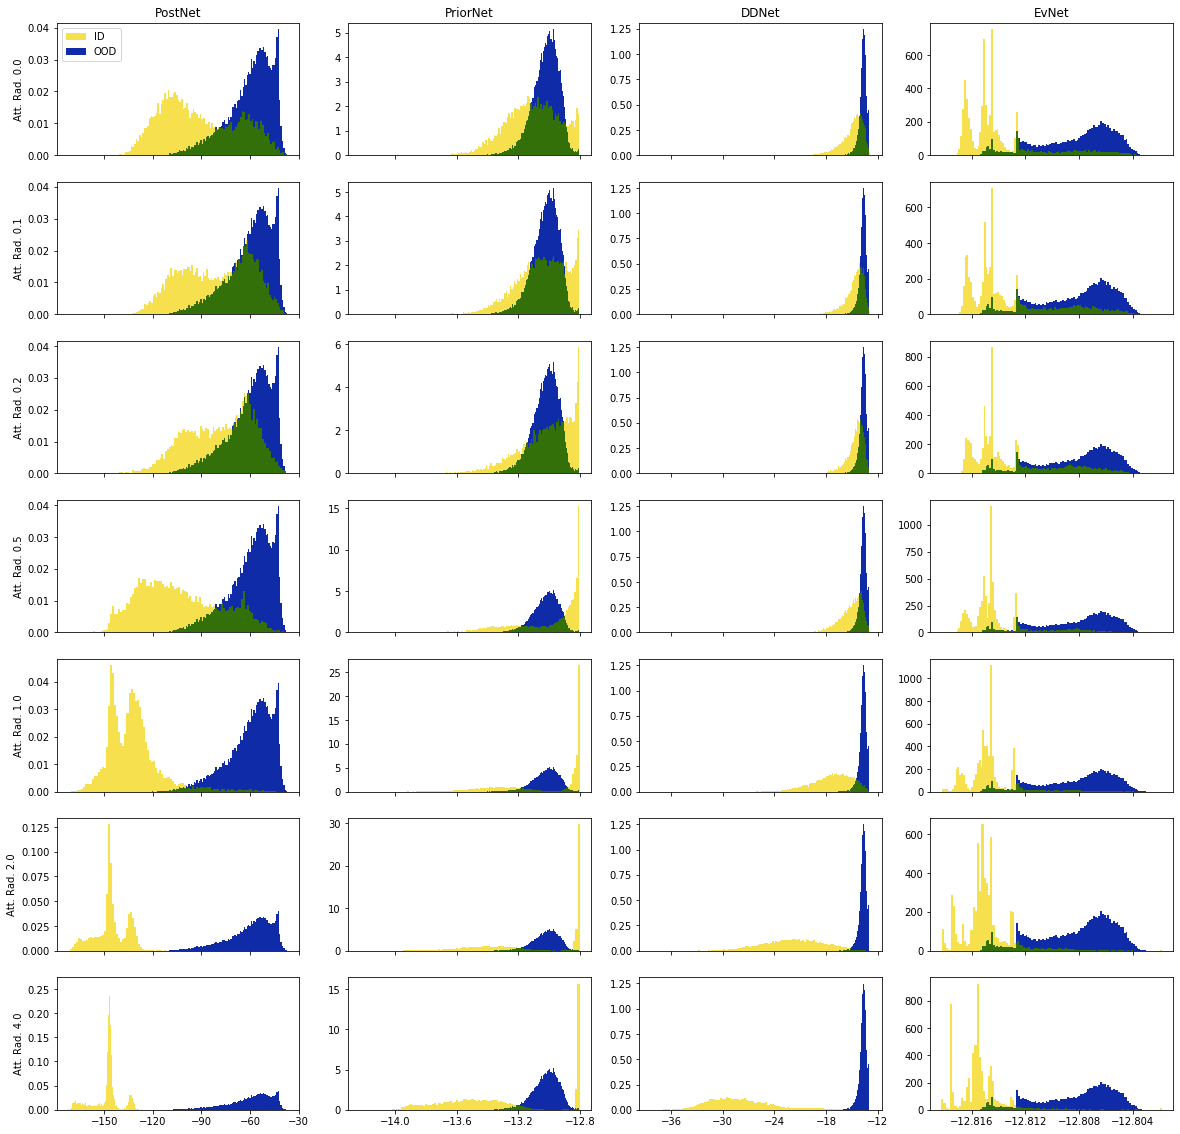
\includegraphics[width=0.99 \textwidth]{sections/008_icml2021/eval/unc_dist_label_id_cifar10_c.png}
    \end{subfigure}%
    \caption{Visualization of the differential entropy distribution of ID data (CIFAR10) and OOD data (SVHN) under label attack. The first row corresponds to no attack. The other rows correspond do increasingly stronger attack strength.}
    \label{fig:attaked_samples_idood_label_attacks_2}
	\vspace{-.5cm}
\end{figure*}
\newpage

\begin{figure*}[ht!]
    \centering
        \begin{subfigure}[t]{1.0\textwidth}
        \centering
        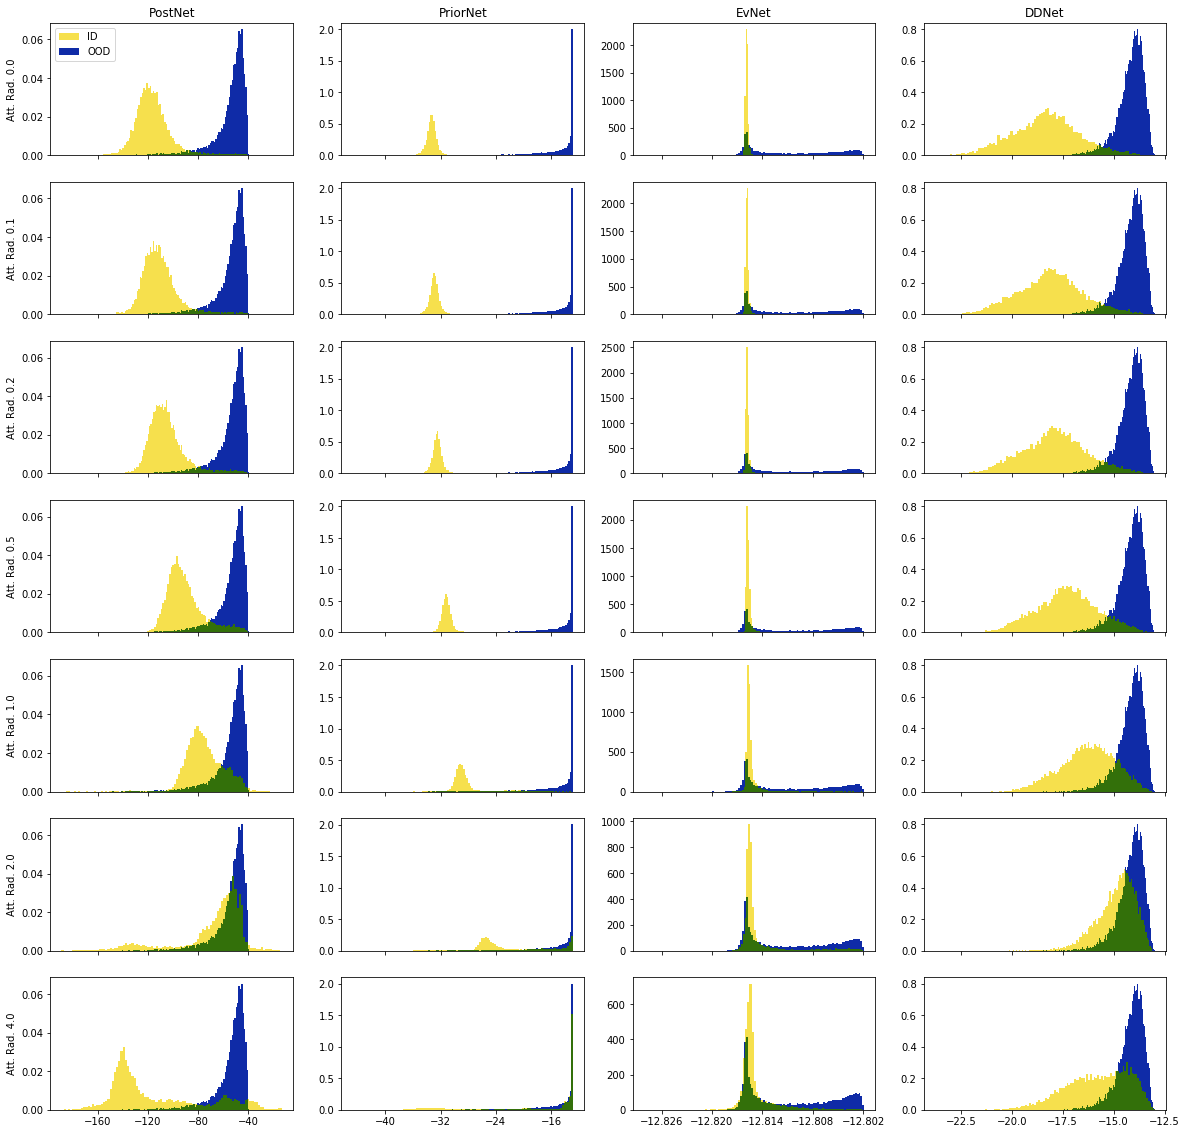
\includegraphics[width=0.99 \textwidth]{sections/008_icml2021/eval/unc_dist_label_id_mnist_c.png}
    \end{subfigure}%
    \caption{Visualization of the differential entropy distribution of ID data (MNIST) and OOD data (KMNIST) under label attack. The first row corresponds to no attack. The other rows correspond do increasingly stronger attack strength.}
    \label{fig:attaked_samples_idood_label_attacks_3}
	\vspace{-.5cm}
\end{figure*}
\newpage

\begin{figure*}[ht!]
    \centering
        \begin{subfigure}[t]{1.0\textwidth}
        \centering
        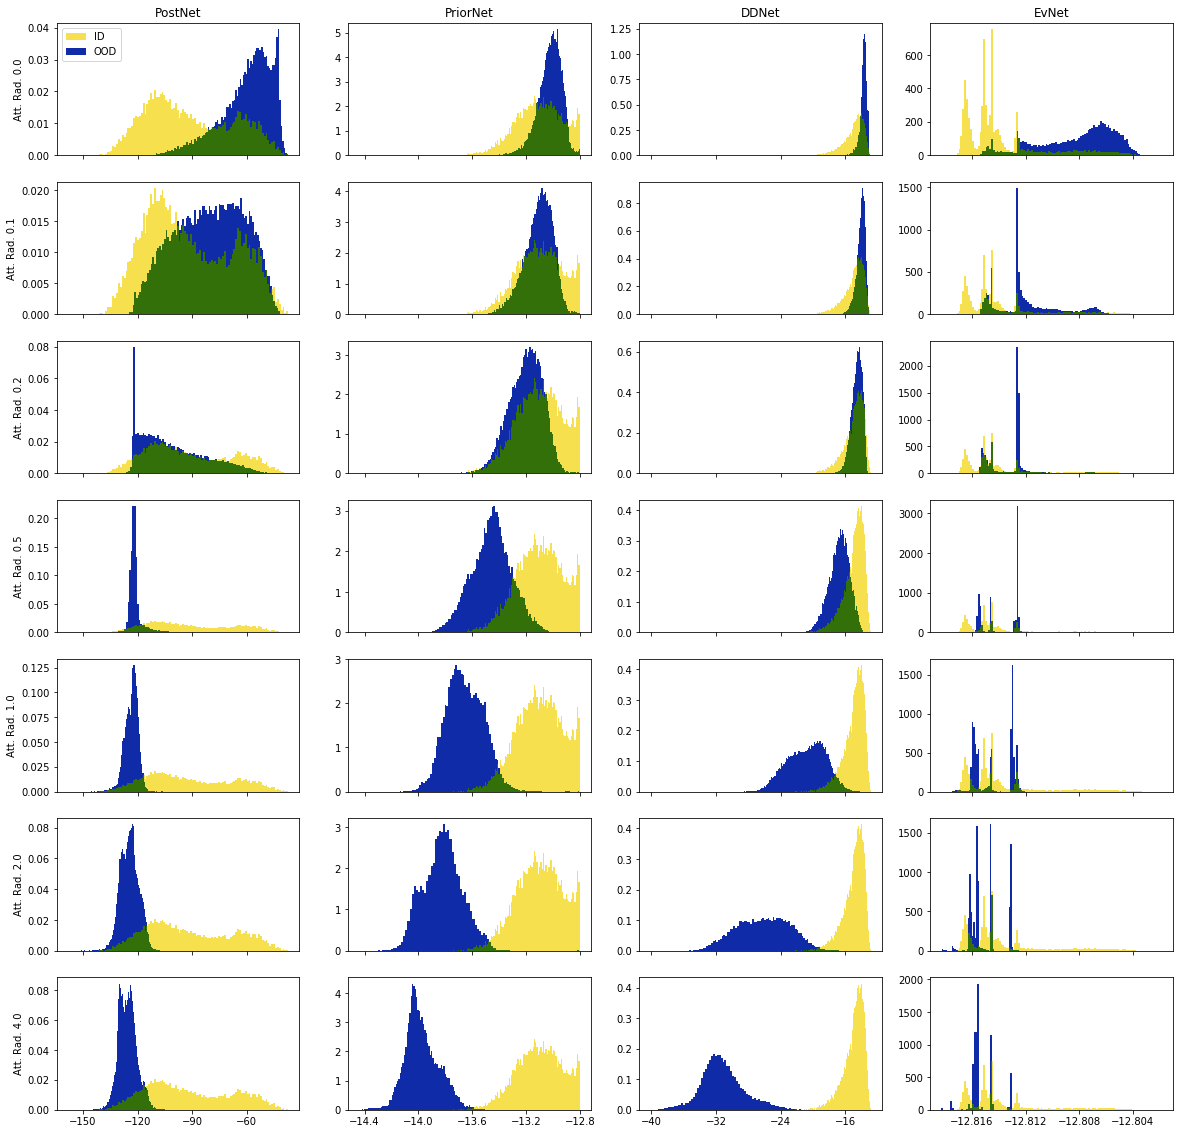
\includegraphics[width=0.99 \textwidth]{sections/008_icml2021/eval/unc_dist_unc_ood_cifar10_c.png}
    \end{subfigure}%
    \caption{Visualization of the differential entropy distribution of ID data (CIFAR10) and OOD data (SVHN) under OOD uncertainty attack. The first row corresponds to no attack. The other rows correspond do increasingly stronger attack strength.}
    \label{fig:attaked_samples_idood_2}
	\vspace{-.5cm}
\end{figure*}


\begin{figure*}[ht!]
    \centering
        \begin{subfigure}[t]{1.0\textwidth}
        \centering
        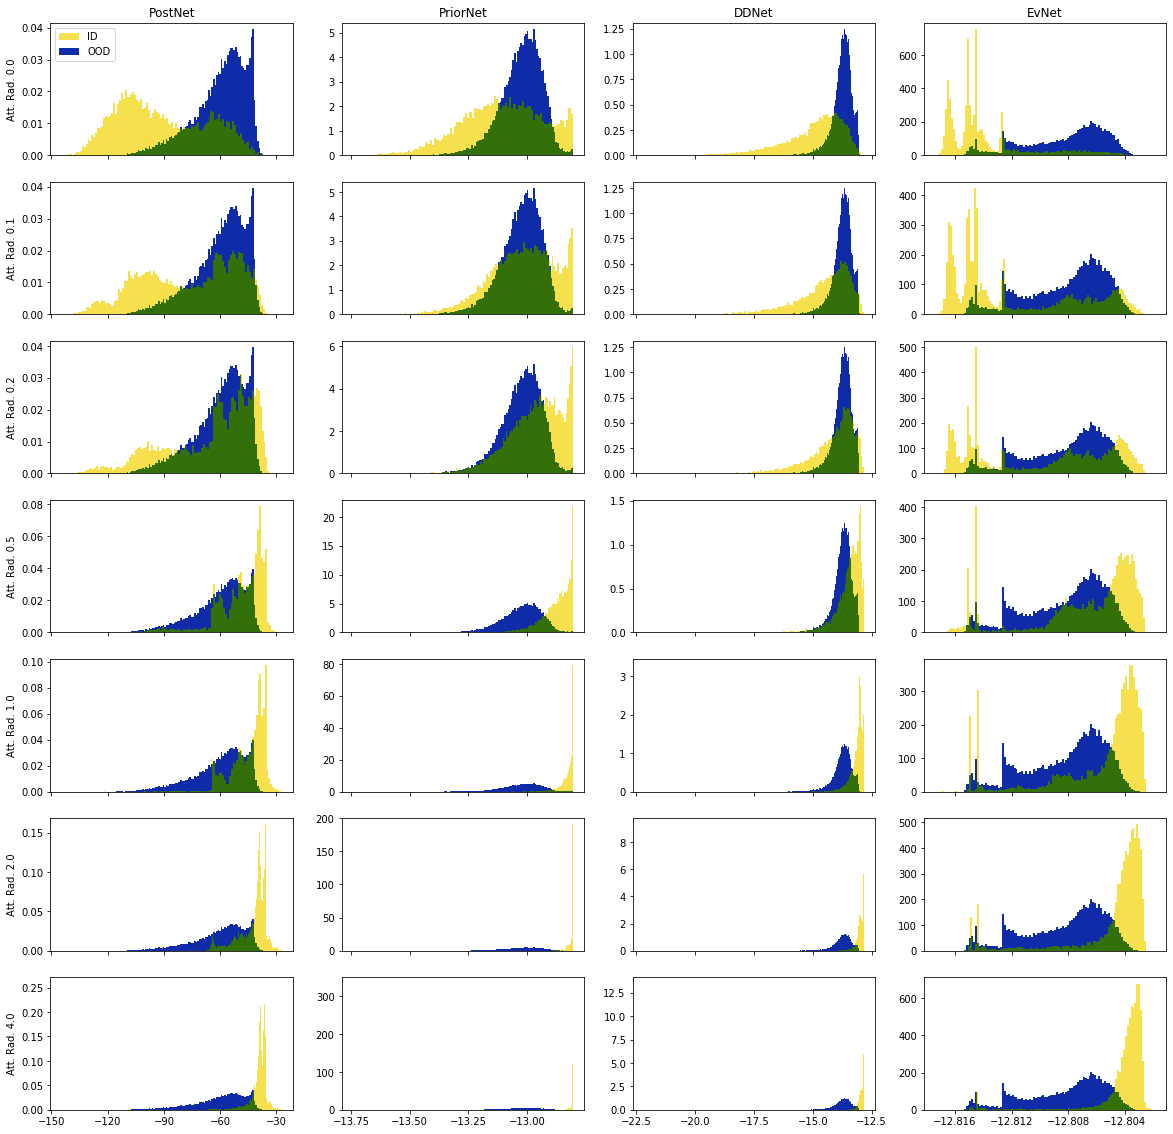
\includegraphics[width=0.99 \textwidth]{sections/008_icml2021/eval/unc_dist_unc_id_cifar10_c.png}
    \end{subfigure}%
    \caption{Visualization of the differential entropy distribution of ID data (CIFAR10) and OOD data (SVHN) under ID uncertainty attack. The first row corresponds to no attack. The other rows correspond do increasingly stronger attack strength.}
    \label{fig:attaked_samples_idood_3}
	\vspace{-.5cm}
\end{figure*}

\begin{figure*}[ht!]
    \centering
        \begin{subfigure}[t]{1.0\textwidth}
        \centering
        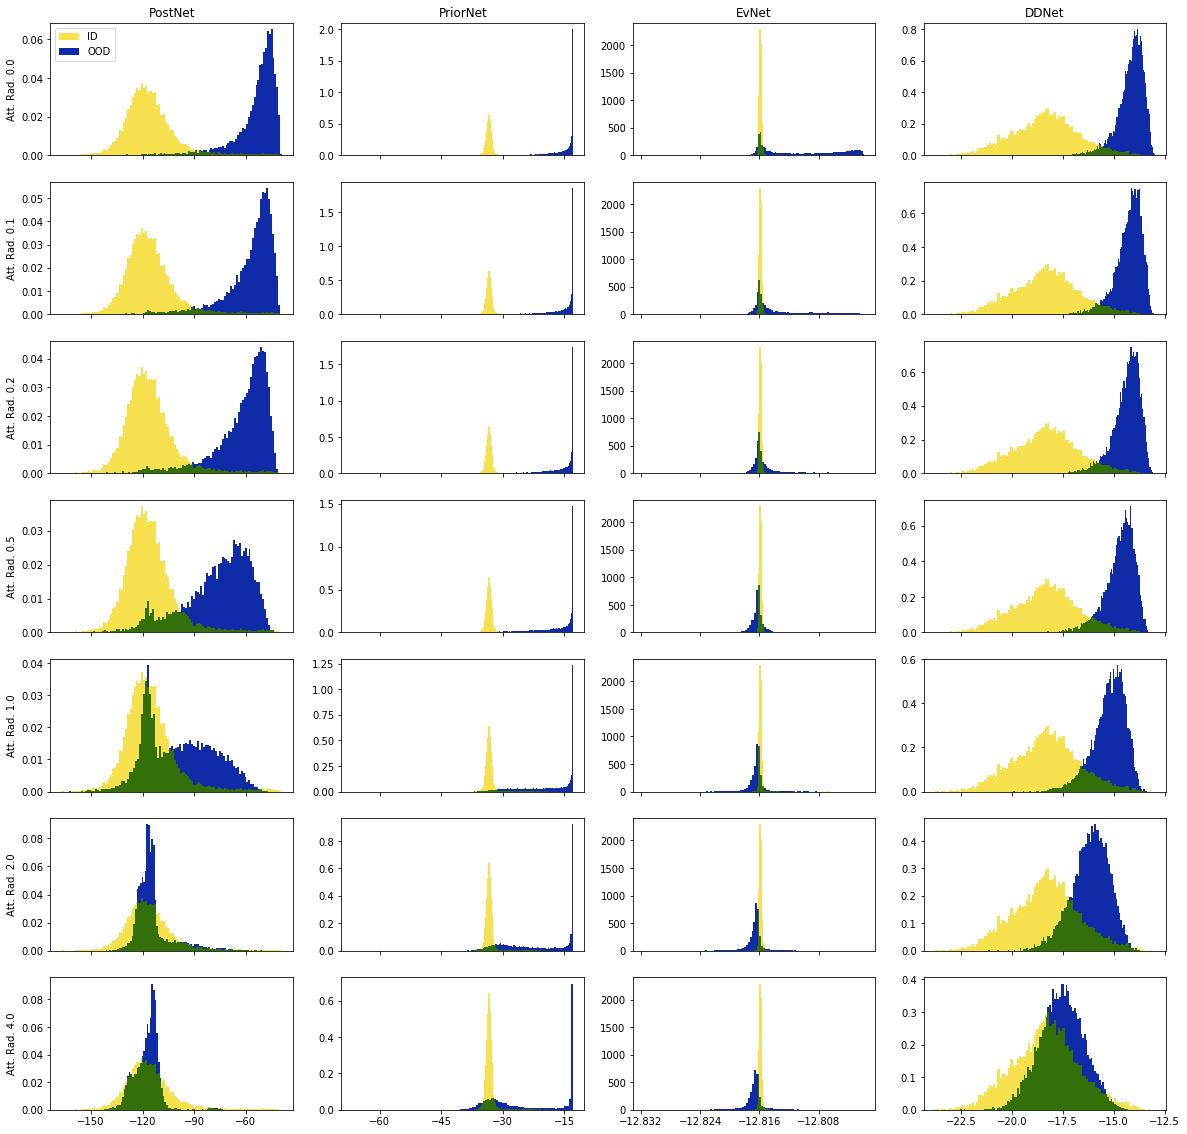
\includegraphics[width=0.99 \textwidth]{sections/008_icml2021/eval/unc_dist_unc_ood_mnist_c.png}
    \end{subfigure}%
    \caption{Visualization of the differential entropy distribution of ID data (MNIST) and OOD data (KMNIST) under OOD uncertainty attack. The first row corresponds to no attack. The other rows correspond do increasingly stronger attack strength.}
    \label{fig:attaked_samples_idood_mnist}
	\vspace{-.5cm}
\end{figure*}


\begin{figure*}[ht!]
    \centering
        \begin{subfigure}[t]{1.0\textwidth}
        \centering
        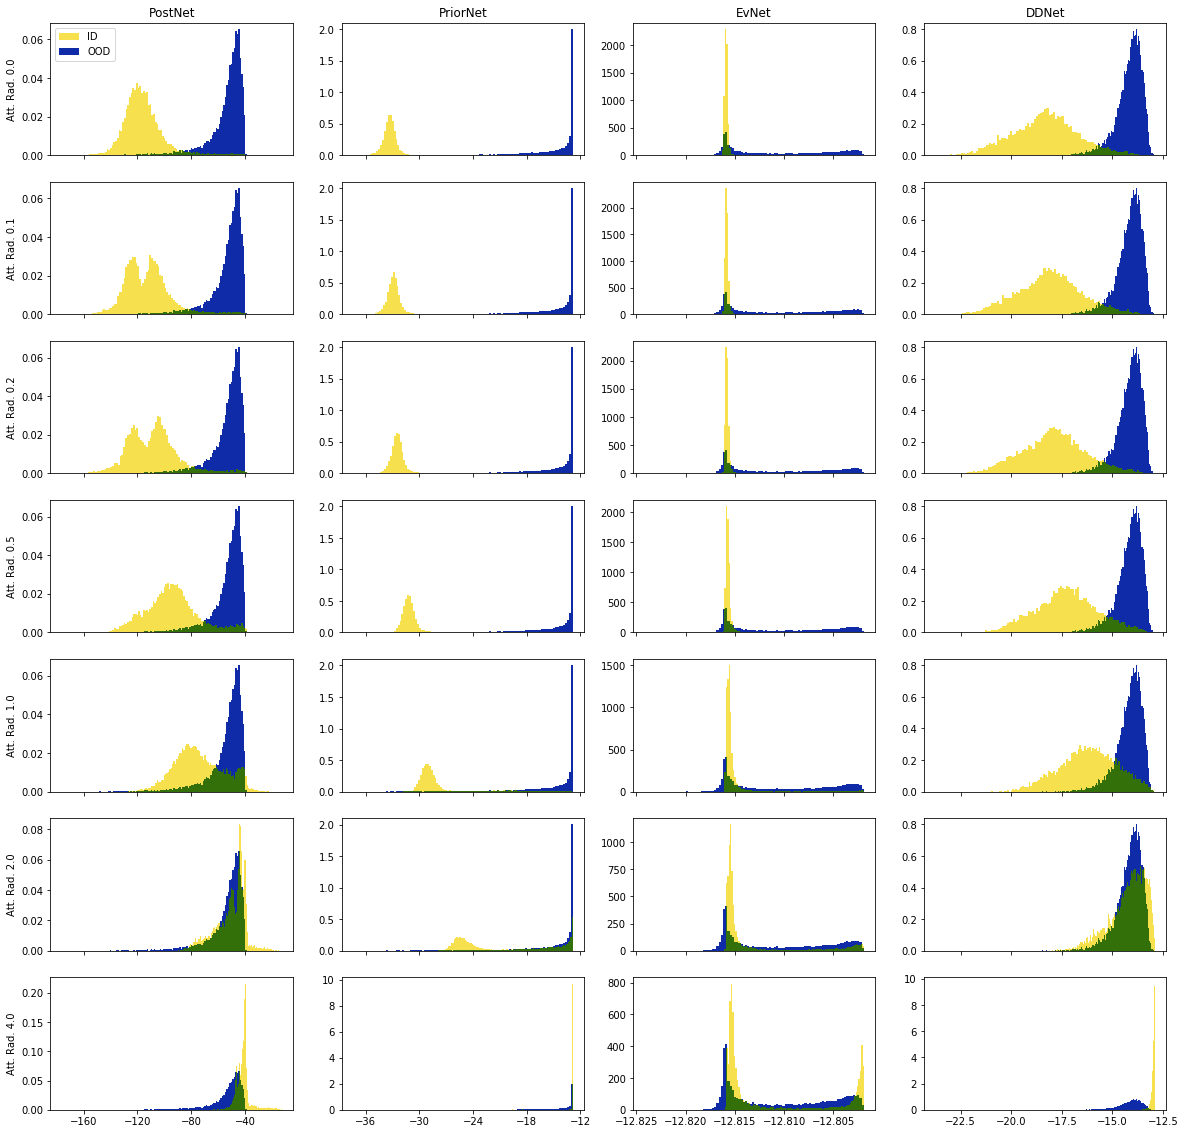
\includegraphics[width=0.99 \textwidth]{sections/008_icml2021/eval/unc_dist_unc_id_mnist_c.png}
    \end{subfigure}%
    \caption{Visualization of the differential entropy distribution of ID data (MNIST) and OOD data (KMNIST) under ID uncertainty attack. The first row corresponds to no attack. The other rows correspond do increasingly stronger attack strength.}
    \label{fig:attaked_samples_idood_mnist_2}
	\vspace{-.5cm}
\end{figure*}









%%%%%%%%%%%%%%%%%%%%%%%%%%%%%%%%%%%%%%%%%%%%%%%%%%%%%%%%%%%%%%%%%%%%%%%%%%%%%%%
%%%%%%%%%%%%%%%%%%%%%%%%%%%%%%%%%%%%%%%%%%%%%%%%%%%%%%%%%%%%%%%%%%%%%%%%%%%%%%%
% DELETE THIS PART. DO NOT PLACE CONTENT AFTER THE REFERENCES!
%%%%%%%%%%%%%%%%%%%%%%%%%%%%%%%%%%%%%%%%%%%%%%%%%%%%%%%%%%%%%%%%%%%%%%%%%%%%%%%
%%%%%%%%%%%%%%%%%%%%%%%%%%%%%%%%%%%%%%%%%%%%%%%%%%%%%%%%%%%%%%%%%%%%%%%%%%%%%%%
%\appendix
%\section{Do \emph{not} have an appendix here}

%\textbf{\emph{Do not put content after the references.}}
%
%Put anything that you might normally include after the references in a separate
%supplementary file.

%We recommend that you build supplementary material in a separate document.
%If you must create one PDF and cut it up, please be careful to use a tool that
%doesn't alter the margins, and that doesn't aggressively rewrite the PDF file.
%pdftk usually works fine. 

%\textbf{Please do not use Apple's preview to cut off supplementary material.} In
%previous years it has altered margins, and created headaches at the camera-ready
%stage. 
%%%%%%%%%%%%%%%%%%%%%%%%%%%%%%%%%%%%%%%%%%%%%%%%%%%%%%%%%%%%%%%%%%%%%%%%%%%%%%%
%%%%%%%%%%%%%%%%%%%%%%%%%%%%%%%%%%%%%%%%%%%%%%%%%%%%%%%%%%%%%%%%%%%%%%%%%%%%%%%


\end{document}


% This document was modified from the file originally made available by
% Pat Langley and Andrea Danyluk for ICML-2K. This version was created
% by Iain Murray in 2018, and modified by Alexandre Bouchard in
% 2019 and 2020. Previous contributors include Dan Roy, Lise Getoor and Tobias
% Scheffer, which was slightly modified from the 2010 version by
% Thorsten Joachims & Johannes Fuernkranz, slightly modified from the
% 2009 version by Kiri Wagstaff and Sam Roweis's 2008 version, which is
% slightly modified from Prasad Tadepalli's 2007 version which is a
% lightly changed version of the previous year's version by Andrew
% Moore, which was in turn edited from those of Kristian Kersting and
% Codrina Lauth. Alex Smola contributed to the algorithmic style files.
